\documentclass{article}

  % packages
    % basic stuff for rendering math
    \usepackage[letterpaper, top=1in, bottom=1in, left=1in, right=1in]{geometry}
    \usepackage[utf8]{inputenc}
    \usepackage[english]{babel}
    \usepackage{amsmath} 
    \usepackage{amssymb}
    \usepackage{polynom}
    \usepackage{longdivision}

    % extra math symbols and utilities
    \usepackage{mathtools}        % for extra stuff like \coloneqq
    \usepackage{mathrsfs}         % for extra stuff like \mathsrc{}
    \usepackage{centernot}        % for the centernot arrow 
    \usepackage{bm}               % for better boldsymbol/mathbf 
    \usepackage{enumitem}         % better control over enumerate, itemize
    \usepackage{hyperref}         % for hypertext linking
    \usepackage{xr-hyper}
    \usepackage{fancyvrb}          % for better verbatim environments
    \usepackage{newverbs}         % for texttt{}
    \usepackage{xcolor}           % for colored text 
    \usepackage{listings}         % to include code
    \usepackage{lstautogobble}    % helper package for code
    \usepackage{parcolumns}       % for side by side columns for two column code
    

    % page layout
    \usepackage{fancyhdr}         % for headers and footers 
    \usepackage{lastpage}         % to include last page number in footer 
    \usepackage{parskip}          % for no indentation and space between paragraphs    
    \usepackage[T1]{fontenc}      % to include \textbackslash
    \usepackage{footnote}
    \usepackage{etoolbox}

    % for custom environments
    \usepackage{tcolorbox}        % for better colored boxes in custom environments
    \tcbuselibrary{breakable}     % to allow tcolorboxes to break across pages

    % figures
    \usepackage{pgfplots}
    \pgfplotsset{compat=1.18}
    \usepackage{float}            % for [H] figure placement
    \usepackage{tikz}
    \usepackage{tikz-cd}
    \usepackage{circuitikz}
    \usetikzlibrary{arrows}
    \usetikzlibrary{positioning}
    \usetikzlibrary{calc}
    \usepackage{graphicx}
    \usepackage{caption} 
    \usepackage{subcaption}
    \captionsetup{font=small}

    % for tabular stuff 
    \usepackage{dcolumn}

    \usepackage[nottoc]{tocbibind}
    \pdfsuppresswarningpagegroup=1
    \hfuzz=5.002pt                % ignore overfull hbox badness warnings below this limit

  % New and replaced operators
    \let\lbrack\relax
    \let\rbrack\relax
    \let\Char\relax
    \let\O\relax
    \newcommand{\lbrack}{[}
    \newcommand{\rbrack}{]}
    \DeclareMathOperator{\Char}{char}
    \DeclareMathOperator{\Tr}{Tr}
    \DeclareMathOperator{\Tran}{Tran}
    \DeclareMathOperator{\Sym}{Sym}
    \DeclareMathOperator{\Span}{span}
    \DeclareMathOperator{\Aut}{Aut}
    \DeclareMathOperator{\End}{End}
    \DeclareMathOperator{\im}{Im}
    \DeclareMathOperator{\ev}{ev}
    \DeclareMathOperator{\Dih}{Dih}
    \DeclareMathOperator{\O}{O}
    \DeclareMathOperator{\sign}{sgn}
    \DeclareMathOperator{\SO}{SO}
    \DeclareMathOperator{\Div}{div}
    \DeclareMathOperator{\ord}{ord}
    \DeclareMathOperator{\curl}{curl}
    \DeclareMathOperator{\Isom}{Isom}
    \DeclareMathOperator{\GL}{GL}
    \DeclareMathOperator{\SU}{SU}
    \DeclareMathOperator{\SL}{SL}
    \DeclareMathOperator{\GA}{GA}
    \DeclareMathOperator{\std}{std}
    \DeclareMathOperator{\Cov}{Cov}
    \DeclareMathOperator{\Var}{Var}
    \DeclareMathOperator{\Corr}{Corr}
    \DeclareMathOperator{\Int}{Int}
    \DeclareMathOperator{\Id}{Id}
    \DeclareMathOperator{\Lie}{Lie}
    \DeclareMathOperator{\Hom}{Hom}
    \DeclareMathOperator{\Alt}{Alt}
    \DeclareMathOperator{\rank}{rank}
    \DeclareMathOperator{\conv}{conv}
    \DeclareMathOperator{\aff}{aff}
    \DeclareMathOperator{\arccot}{arccot}
    \DeclareMathOperator*{\argmin}{\arg\!\min}
    \DeclareMathOperator*{\argmax}{\arg\!\max}
    \newcommand{\qed}{\hfill$\blacksquare$}     % I like QED squares to be black

  % Custom Environments
    \newtcolorbox[auto counter, number within=section]{question}[1][]
    {
      colframe = orange!25,
      colback  = orange!10,
      coltitle = orange!20!black,  
      breakable, 
      title = \textbf{Question \thetcbcounter ~(#1)}
    }

    \newtcolorbox[auto counter, number within=section]{exercise}[1][]
    {
      colframe = teal!25,
      colback  = teal!10,
      coltitle = teal!20!black,  
      breakable, 
      title = \textbf{Exercise \thetcbcounter ~(#1)}
    }
    \newtcolorbox[auto counter, number within=section]{solution}[1][]
    {
      colframe = violet!25,
      colback  = violet!10,
      coltitle = violet!20!black,  
      breakable, 
      title = \textbf{Solution \thetcbcounter}
    }
    \newtcolorbox[auto counter, number within=section]{lemma}[1][]
    {
      colframe = red!25,
      colback  = red!10,
      coltitle = red!20!black,  
      breakable, 
      title = \textbf{Lemma \thetcbcounter ~(#1)}
    }
    \newtcolorbox[auto counter, number within=section]{theorem}[1][]
    {
      colframe = red!25,
      colback  = red!10,
      coltitle = red!20!black,  
      breakable, 
      title = \textbf{Theorem \thetcbcounter ~(#1)} 
    } 
    \newtcolorbox[auto counter, number within=section]{corollary}[1][]
    {
      colframe = red!25,
      colback  = red!10,
      coltitle = red!20!black,  
      breakable, 
      title = \textbf{Corollary \thetcbcounter ~(#1)}
    } 
    \newtcolorbox[auto counter, number within=section]{proof}[1][]
    {
      colframe = orange!25,
      colback  = orange!10,
      coltitle = orange!20!black,  
      breakable, 
      title = \textbf{Proof. }
    } 
    \newtcolorbox[auto counter, number within=section]{definition}[1][]
    {
      colframe = yellow!25,
      colback  = yellow!10,
      coltitle = yellow!20!black,  
      breakable, 
      title = \textbf{Definition \thetcbcounter ~(#1)}
    } 
    \newtcolorbox[auto counter, number within=section]{example}[1][]
    {
      colframe = blue!25,
      colback  = blue!10,
      coltitle = blue!20!black,  
      breakable, 
      title = \textbf{Example \thetcbcounter ~(#1)}
    } 
    \newtcolorbox[auto counter, number within=section]{code}[1][]
    {
      colframe = green!25,
      colback  = green!10,
      coltitle = green!20!black,  
      breakable, 
      title = \textbf{Code \thetcbcounter ~(#1)}
    } 

    \definecolor{dkgreen}{rgb}{0,0.6,0}
    \definecolor{gray}{rgb}{0.5,0.5,0.5}
    \definecolor{mauve}{rgb}{0.58,0,0.82}
    \definecolor{lightgray}{gray}{0.93}

    % default options for listings (for code)
    \lstset{
      autogobble,
      frame=ltbr,
      language=C,                           % the language of the code
      aboveskip=3mm,
      belowskip=3mm,
      showstringspaces=false,
      columns=fullflexible,
      keepspaces=true,
      basicstyle={\small\ttfamily},
      numbers=left,
      firstnumber=1,                        % start line number at 1
      numberstyle=\tiny\color{gray},
      keywordstyle=\color{blue},
      commentstyle=\color{dkgreen},
      stringstyle=\color{mauve},
      backgroundcolor=\color{lightgray}, 
      breaklines=true,                      % break lines
      breakatwhitespace=true,
      tabsize=3, 
      xleftmargin=2em, 
      framexleftmargin=1.5em, 
      stepnumber=1
    }

  % Page style
    \pagestyle{fancy}
    \fancyhead[L]{Abstract Algebra}
    \fancyhead[C]{Muchang Bahng}
    \fancyhead[R]{August 2021} 
    \fancyfoot[C]{\thepage / \pageref{LastPage}}
    \renewcommand{\footrulewidth}{0.4pt}          % the footer line should be 0.4pt wide
    \renewcommand{\thispagestyle}[1]{}  % needed to include headers in title page

  % external documents 
    \externaldocument[st-]{../Set_Theory/paper}[../Set_Theory/paper.pdf] 
    \externaldocument[pst-]{../Point_Set_Topology/paper}[../Point_Set_Topology/paper.pdf] 

\begin{document}

\title{Abstract Algebra}
\author{Muchang Bahng}
\date{Spring 2024}

\maketitle
\tableofcontents
\pagebreak 

Unlike my machine learning notes, which focuses mostly on the theoretical soundness of classical (e.g. pre-deep and interpretable) models, the theory of deep neural networks have not been developed as well yet. Furthermore, the recency of developments, especially in the post-2010s, results in a pretty nonlinear\footnote{No pun intended.} timeline that is difficult to categorize effectively. Before I give my motivation, the direct prerequisites for deep learning are basic knowledge of my notes in probability theory, machine learning, and real analysis. 

Therefore, after much thought, I think organizing my notes in chronological order would be best. It turned out that in the early days of deep learning, most researchers like Andrew Ng stated that he focused on supervised models,\footnote{He states this in his podcast with Lex Fridman.} and it wasn't until the 2010s that the development of unsupervised models burgeoned. 

\begin{enumerate}
  \item We start by introducing \textit{multilayered perceptrons} (MLPs), which build upon generalized linear models (GLMs) that we have went over in machine learning. This is pretty much the ``foundational'' model that we will build on. We then talk a about practical methodologies regarding training and control. 

  \item Then we introduce the other two architectures. The \textit{convolutional neural network} (CNN) gives us a scalable way to perform sparse matrix multiplication efficiently, by taking advantage of locality. Then in \textit{recurrent neural networks} (RNNs), we are not limited to a single $n$-dimensional vector input and are able to process a time series of inputs.  
    
  \item With these building blocks, we are able take and two neural networks together to create an encoder-decoder model. The two main applications of this was dimensionality reduction with \textit{autoencoders}, followed by \textit{seq2seq} for machine translation between sequences of words.  

  \item The practical success of autoencoders led to the development of not just density estimation models, but \textit{generative} ones that seek to sample from the learned distribution. These generative models were ``deep'' extensions of the classical linear factor models resulting in \textit{restricted Boltzmann machines (RBMs)} and \textit{variational autoencoders (VAEs)}, which attempted to explicitly model an approximation of the true data generating distribution. More specifically, RBMs were \textit{energy models} that borrowed ideas from physics to learn a distribution of the form $p_X (x) = \frac{1}{Z} e^{-f_\theta (x)}$. To sample from this, researchers already had access to the established Markov Chain Monte Carlo (MCMC) algorithms designed for this exact problem. As for VAEs, these were trained and sampled through \textit{variational inference} methods. 

  \item In 2014, a completely new architecture composed of 2 neural networks competing each other gave rise to \textit{generative adversarial networks} (GANs) which blew RBMs and VAEs away. A similar architecture followed with \textit{generative stochastic networks} (GSNs).

  \item In 2016, \textit{normalizing flow models}, which attempted to model a smooth function that transformed simple latent variables to the true data generating distribution, were invented by Google DeepMind and surpassed GANs. 

  \item In 2017, \textit{attention} took the world by storm, which had drastically improved machine translation in seq2seq, and the resulting \textit{self-attention} plus the \textit{transformer} architectures led to the success of OpenAI's ChatGPT. 
\end{enumerate} 

Again, I emphasize that the math in these notes are not very advanced. However, implementing these simple models and training algorithms from scratch is a challenge in itself. I will go through implementing everything from scratch as if we were building a mini-version of PyTorch as we learn new topics. My implementations can be found \href{https://github.com/mbahng/pyember}{here}. 

\section{Group-Like Structures} 

\subsection{Semigroups and Monoids}

  Now the endowment of some structures gives rise to the following. Usually, we will start with the most general algebraic structures and then as we endow them with more structure, we can prove more properties. 

  \begin{definition}[Semigroup]
    A \textbf{semigroup} $(S, *)$ is a set $S$ with an associative binary operation. 
  \end{definition} 

  \begin{definition}[Monoid]
    A \textbf{monoid} $(M, *)$ is a semigroup with an identity element $1 \in M$ such that given a $m \in M$
    \begin{equation}
      1 * m = m * 1 = m
    \end{equation}
  \end{definition}

  Groupoids aren't necessarily that interesting, but there are cases in which semigroups and monoids come up. 

  \begin{example}[Continuous Time Markov Chain]
    Let $(\Omega, \mathcal{F}, \mathbb{P})$ be a probability space and $(S, \mathcal{S})$ a measurable space. Then, a homogeneous continuous-time Markov chain is a stochastic process $\{X_t\}_{t \geq 0}$ taking values in $S$ (i.e. $X_t: \Omega \rightarrow S$) satisfying the \textbf{Markov property}: for every bounded measurable $f$ and and $t, s \geq 0$, 
    \begin{equation}
      \mathbb{E}[ f(X_{t + s}) \mid \{X_r\}_{r \leq t} ] = \mathbb{E}[ f(X_{t + s}) \mid X_t ] = (P_s f)(X_t)
    \end{equation}
    The set $\{P_t\}_{t \geq 0}$ is called the \textbf{Markov semigroup}. 
  \end{example} 

  \begin{example}[Monoid of Transformations]
    Given a set $S$, consider the set of all functions $f: S \rightarrow S$. This forms a monoid with the identity function $f(x) = x$ as the identity element. Proof of associativity is shown in my set theory notes. 
  \end{example} 

  \begin{theorem}[Cardinality of Monoid of Transformations]
    If $|S| = n$, then the monoid of transformations has cardinality $n^n$. 
  \end{theorem}

  \begin{example}
    Let $S$ be any nonempty set. Then $(2^S, \cup, \emptyset)$ and $(2^S, \cap, S)$ are monoids. 
  \end{example}

  We first should ask whether the identity is unique in a monoid. It turns out it is. 

  \begin{lemma}[Uniqueness of Monoid Identity]
    The identity $1$ of a monoid $M$ is unique. 
  \end{lemma}
  \begin{proof}
    Assume not, i.e. there are 2 identities $1 \neq 1^\prime$. But then 
    \begin{equation}
      1 = 1 1^\prime = 1^\prime \implies 1 = 1^\prime
    \end{equation}
    where the implication follows from transitivity of equivalence relations. 
  \end{proof} 

  \begin{definition}[Submonoid]
    Given a monoid $(M, \ast)$, let $M^\prime \subset M$. If the restriction of $\ast$ to $M^\prime \times M^\prime$ is closed in $M^\prime$, then we can define the \textbf{submonoid} $(M^\prime, \ast)$. 
  \end{definition} 

  \begin{theorem}[Identities of Submonoids]
    If $M^\prime$ with identity $1^\prime$ is a submonoid of $M$ with identity $1$, Then $1 = 1^\prime$. 
  \end{theorem}
  \begin{proof}
    Assume not. $1^\prime \in M$, which means that 
  \end{proof}

\subsection{Groups}
  
  \begin{definition}[Group]
    A \textbf{group} $(G, \ast)$ is a set with binary operation $x \ast y$---also written as $xy$---having the following properties.\footnote{Note that this is a monoid with the additional property of inverses.}
    \begin{enumerate}
      \item \textit{Closure}. $x, y \in G \implies xy \in G$\footnote{but not necessarily $xy  = yx$}
      \item \textit{Associativity}. $\forall x, y, z \in G, x(yz) = (xy)z$
      \item \textit{Identity}. $\exists e \in G$ s.t. $\forall x \in G, xe = ex = x$
      \item \textit{Inverses}. $\forall x \in G \; \exists x^{-1} \in G$ s.t. $x x^{-1} = x^{-1} x = e$
    \end{enumerate}
    The \textbf{order} of a group is the cardinality $|G|$. 
  \end{definition} 

  This is an extremely simple structure, and the first thing we should prove is the uniqueness of the identity and inverses. 

  \begin{lemma}[Uniqueness of Identity and Inverse]
    The identity and the inverse is unique, and for any $a, b$, the equation $x*a = b$ has the unique solution $x = b* a^{-1}$.
  \end{lemma}
  \begin{proof}
     Assume that there are two identities of group $(G,*)$, denoted $e_{1}, e_{2}$, where $e_{1} \neq e_{2}$. According to the properties of identities, $e_{1} = e_{1} * e_{2} = e_{2} \implies e_{1} = e_{2}$. \\
    As for uniqueness of a inverses, let $a$ be an element of $G$, with its inverses $a_{1}^{-1}, a_{2}^{-1}$. Then, 
    \begin{align*}
      a * a_{1}^{-1} = e & \implies a_{2}^{-1} * \Big(a * a_{1}^{-1} \Big)= a_{2}^{-1} * e \\
       & \implies \Big(a_{2}^{-1} * a \Big) * a_{1}^{-1} = a_{2}^{-1} \\
       & \implies e * a_{1}^{-1} = a_{2}^{-1}
    \end{align*}
    Since the inverse is unique, we can operate on each side of the equation $x*a = b$ to get $x*a*a^{-1} = b*a^{1} \implies x * e = x = b*a^{-1}$. Clearly, the derivation of this solution is unique since the elements that we have operated on are unique.
  \end{proof} 
  
  At this point, we can see that for each group there is a corresponding ``multiplication table'' defined by the operation. For example, we can create a set of $6$ elements $\{r_0, r_1, r_2, s_0, s_1, s_2\}$ and define the operation $\times$ as the following. 

  \begin{figure}[H]
    \centering 
    \begin{tabular}{c|cccccc}
      $\times$ & $r_0$ & $r_1$ & $r_2$ & $s_0$ & $s_1$ & $s_2$ \\
      \hline
      $r_0$ & $r_0$ & $r_1$ & $r_2$ & $s_0$ & $s_1$ & $s_2$ \\
      $r_1$ & $r_1$ & $r_2$ & $r_0$ & $s_1$ & $s_2$ & $s_0$ \\
      $r_2$ & $r_2$ & $r_0$ & $r_1$ & $s_2$ & $s_0$ & $s_1$ \\
      $s_0$ & $s_0$ & $s_2$ & $s_1$ & $r_0$ & $r_2$ & $r_1$ \\
      $s_1$ & $s_1$ & $s_0$ & $s_2$ & $r_1$ & $r_0$ & $r_2$ \\
      $s_2$ & $s_2$ & $s_1$ & $s_0$ & $r_2$ & $r_1$ & $r_0$ \\
    \end{tabular}
    \caption{Multiplication table for some random (or is it?) group. Note that we can only write such a table explicitly for a group of finite elements. But even for arbitrary groups, we should think of the operation completely defining a possibly ``infinite'' table.} 
  \end{figure} 

  \begin{example}[Group of Invertible Elements of a Monoid]
    
  \end{example}

  Let's prove a little more about groups so that we have more tools for manipulation. 

  \begin{lemma}[Properties of Group Operation]
    Given $a, b, c \in G$, 
    \begin{enumerate}
      \item $ab = cb \implies a = c$. 
      \item $\forall a \in G$, $(a^{-1})^{-1} = a$. 
      \item $(ab)^{-1} = b^{-1} a^{-1}$. 
    \end{enumerate}
  \end{lemma}
  \begin{proof}
    TBD. 
  \end{proof}

  \begin{definition}[Subgroup]
    Given group $(G, \ast)$ and $(G^\prime, \ast)$ with the same operations, $G^\prime$ is a \textbf{subgroup} of $G$ if $G^\prime \subset G$. 
  \end{definition} 

  \begin{definition}[Abelian Group]
    An \textbf{abelian group} $(A, +)$ is a group where $+$ is commutative.\footnote{Note that I switched the notation from $\ast$ to $+$. By convention and to avoid confusion, $+$ denotes commutative operations. }
  \end{definition} 

  It is clear that in an abelian group, the multiplication table must be symmetric across the diagonal. 

  \begin{example}[Abelian Groups]
    Here are some examples. 
    \begin{enumerate}
      \item $\mathbb{Z}, \mathbb{Q}, \mathbb{R}$ are all abelian groups with respect to addition. $\mathbb{Q}^{*} \equiv \mathbb{Q} \setminus \{0\}$ and $\mathbb{R}^{*} \equiv \mathbb{R} \setminus \{0\}$ are abelian groups with respect to multiplication.
      \item The set of all functions on a given interval $[a,b]$ is abelian with respect to addition, defined as $(f+g)(x) \equiv f(x) + g(x)$. 
    \end{enumerate}
  \end{example} 

\subsection{Group Homomorphisms}

  At this point, we would like to try and classify groups (e.g. can we find \textit{all} possible groups of a finite set?). But consider the two groups. 

  \begin{figure}[H]
    \centering
    \begin{subfigure}[b]{0.48\textwidth}
      \centering
      \begin{tabular}{c|ccc}
        \hline
        $+$ & 0 & 1 & 2 \\
        \hline
        0 & 0 & 1 & 2 \\
        1 & 1 & 2 & 0 \\
        2 & 2 & 0 & 1 \\
        \hline
      \end{tabular}
    \end{subfigure}
    \hfill 
    \begin{subfigure}[b]{0.48\textwidth}
      \centering
      \begin{tabular}{c|ccc}
        \hline
        $+$ & a & b & c \\
        \hline
        a & a & b & c \\
        b & b & c & a \\
        c & c & a & b \\
        \hline
      \end{tabular}
    \end{subfigure}
    \caption{Two isomorphic groups.}
  \end{figure} 

  These groups have different elements, but the operation behaves in exactly the same way between them (it may be a little harder if I relabeled the elements or permuted the rows/columns). Since we can trivially make arbitrary sets there really isn't much meaning to having two versions of the same group (at least in the algebraic sense). Therefore, these groups should be labeled ``equivalent'' in some way, and we will precisely define this notion now. 

  \begin{definition}[Group Homomorphism]
    Let $(G, \circ)$ and $(H, *)$ be two groups. The mapping $f: (G, \circ) \longrightarrow (H, *)$ is a \textbf{group homomorphism} if for all $a, b \in G$, 
    \begin{equation}
      f(a \circ b) = f(a) * f(b)
    \end{equation} 
    Furthermore, 
    \begin{enumerate}
      \item A \textbf{group isomorphism} is a bijective group homomorphism, and we call groups $M, N$ \textbf{isomorphic}, denoted $M \simeq N$, if there exists an isomorphism between them. 
      \item An \textbf{endomorphism} is a homomorphism from a group to itself. 
      \item An \textbf{automorphism} is a isomorphism from a group to itself. 
    \end{enumerate}
  \end{definition} 

  It turns out that from the simple property that $f(ab) = f(a) f(b)$, it also maps identities to identities, and inverses to inverses!  

  \begin{lemma}[Homomorphisms Maps Identities/Inverses to Identities/Inverses]
    Given a homomorphism $f: (G, \ast) \rightarrow (H, \times)$ and $a \in G$, 
    \begin{equation}
      f(e_G) = e_H, \qquad f(a^{-1}) = f(a)^{-1}
    \end{equation}
  \end{lemma}
  \begin{proof}
    Let $a \in G$. Then 
    \begin{equation}
      f(a) = f(a e_G) = f(a) f(e_G) \implies e_H = f(a)^{-1} f(a) = f(a)^{-1} f(a) f(e_G) = f(e_G)
    \end{equation}
    To prove inverses, we see that 
    \begin{equation}
      f(a) f(a^{-1}) = f(a a^{-1}) = f(e_G) = e_H
    \end{equation}
    from above, and this implies that $f(a^{-1}) = f(a)^{-1}$. We can also do this with right hand side multiplication. 
  \end{proof}

  \begin{example}[Exponential Map]
    The map $a \mapsto 2^{a}$ is an isomorphism between $(\mathbb{R}, +)$ and $(\mathbb{R}^{+}, \times)$ since 
    \begin{equation}
      2^{a+b} = 2^a \times 2^b
    \end{equation} 
    which is proved in my real analysis notes when constructing the exponential map on the reals. 
  \end{example} 

  \begin{example}[Determinant]
    The determinant $\det: \GL_n (\mathbb{F}) \rightarrow \mathbb{F}^\ast$ is a homomorphism because of the product rule for determinants. 
  \end{example}

  Therefore, we can see that an isomorphism is really just a ``renaming'' of the elements, which aligns with our view of equivalence as above. Not only does it renamee the elements, but it preserves all the algebraic properties of the group and each element. 

  \begin{theorem}[Preservation of Properties in Isomorphism]
    If $f: G \rightarrow H$ is an isomorphism, then 
    \begin{enumerate}
      \item $f^{-1}$ is also an isomorphism. 
      \item $|G| = |H|$.
      \item $\forall a \in G$, $\ord(a) = \ord(f(a))$. 
      \item $G$ is abelian $\implies H$ is abelian. 
    \end{enumerate} 
  \end{theorem}
  \begin{proof}
    Listed. 
    \begin{enumerate}
      \item Since $f$ is bijective by definition, $f^{-1}$ is well-defined and bijective as well. Now we show that $f^{-1}$ is a group homomorphism. Given $c, d \in H$, take 
      \begin{equation}
        f \big( f^{-1} (c), f^{-1} (d)\big) = f \big( f^{-1} (c) \big) \, f \big( f^{-1} (d) \big) = cd 
      \end{equation}
      where the first equality follows since $f$ is a homomorphism, and the second since $f^{-1}$ is the inverse mapping. Now mapping both sides through $f^{-1}$, we get 
      \begin{equation}
        f^{-1} (c) f^{-1} (d) = f^{-1} (cd)
      \end{equation}
      and so $f^{-1}$ is a homomorphism. 

      \item This is trivial by bijectivity. 
      \item TBD. 
      \item Let $c, d \in H$. Then $c = f(a), d = f(b)$ for some $a, b \in G$, and so $cd = f(a) f(b) = f(ba) = f(b) f(a) = dc$. 
    \end{enumerate}
  \end{proof}

  A trivial example is the identity map, which is an automorphism. But can we generalize this a bit better? 

  \begin{theorem}
    Let $G$ be a group with $a \in G$. Then the following is an automorphism on $G$. 
    \begin{equation}
      \phi: G \longrightarrow G, \; \phi (x) = a x a^{-1}
    \end{equation}
  \end{theorem}
  \begin{proof}
    The map $\psi: G \longrightarrow G, \; \psi(x) = a^{-1} x a$ is clearly the inverse of $\phi$, with $\phi \psi = \psi \phi = I$ for all $x \in G \implies \phi$ is bijective. Secondly, $\phi(x) \phi(y) = a x a^{-1} a y a^{-1} = a (x y) a ^{-1} = \phi (x y) \implies \phi$ preserves the group structure. 
  \end{proof} 

  \begin{definition}[Kernel]
    Given group homomorphism $f: G \rightarrow H$, the \textbf{kernel} of $f$ is defined 
    \begin{equation}
      \ker(f) \coloneqq \{g \in G \mid f(g) = e_H\}
    \end{equation}
    That is, it is the preimage of the identity. 
  \end{definition} 

  \begin{theorem}[Kernels are Subgroup]
    Given a group homomorphism $f: G \rightarrow H$, 
    \begin{enumerate}
      \item $\ker(f)$ is a subgroup of $G$.  
      \item $f$ is injective $\iff \ker(f) = \{e_G\}$. 
    \end{enumerate}
  \end{theorem}
  \begin{proof}
    For the first part, we prove the properties of a group. To show closed, consider $a, b \in \ker(f)$. Then $f(ab) = f(a) f(b) = e_H e_H = e_H \implies ab \in \ker(f)$. Since $f(e_G) = e_H$, $e_G \in \ker(f)$. If $a \in \ker(f)$, then $f(a^{-1}) = f(a)^{-1} = e_H^{-1} = e_H \implies a^{-1} \in \ker(f)$. Finally associativity follows from associativity of the supgroup. 

    For the second part, we prove bidirectionally. 
    \begin{enumerate}
      \item $(\rightarrow)$. Since $f$ is injective, $f(a) = f(b) \implies a = b$. Let $a \in \ker(f)$. Then $f(a) = e_H$, and so $f(e_G) = e_H = f(a)$. By injectivity, $a = e_G$, and so $\ker(f) = \{e_G\}$. 
      \item $(\leftarrow)$. Let $a, b \in G$ s.t. $f(a) = f(b)$. Then $f(a) f(b)^{-1} = e_H \implies af(a) f(b^{-1}) = f(a b^{-1}) = e_H \implies ab^{-1} \in \ker(f)$. But by hypothesis $\ker(f) = \{e_G\} \implies ab^{-1} = e_G \implies a = b$. 
    \end{enumerate}
  \end{proof}

  \begin{example}[Projection onto Unit Circle]
    Given $\mathbb{C}^\ast = \mathbb{C} \setminus \{0\}$ with $\times$ and $S^1 = \{x \in \mathbb{C} \mid |x| = 1\}$ (which is a group under multiplication), the map $f: \mathbb{C}^\ast \rightarrow S^1$ defined $f(z) = z/|z|$ is a group homomorphism since 
    \begin{equation}
      f(z_1 z_2) = \frac{z_1 z_2}{|z_1 z_2|} = \frac{z_1 z_2}{|z_1| |z_2|} = f(z_1) f(z_2)
    \end{equation}
  \end{example} 

\subsection{Group Presentations} 

  A group $G$ may be very abstract and complicated, and so working with all its elements can be a bit painful. It would be more useful to work with a smaller subset $S$ of $G$ that can completely characterize $G$.\footnote{Note that this is similar to the basis that generates a topology.} We would like to formalize this notion, which will be very useful later on. For now, let's start off with a simple element $a \in G$, and perhaps we can consider the elements 
  \begin{equation}
    \ldots, a^{-2}, a^{-1}, a^0 = e, a^1, a^2, \ldots
  \end{equation}
  It may or may not be the case that $a$ may cycle back to itself for some $n$, i.e. $a = a^n$. 

  \begin{definition}[Order of an Element]
    The \textbf{order} of a group element $a \in G$ is the minimum number $n \in \mathbb{N}$ s.t. $a = a^n$, denoted $|a|$ or $\ord(a)$.\footnote{Note that this is different from the order of a group. This is confusing, I know. }
  \end{definition} 

  Now the set of all multiples of $a$ may or may not be the group, but if we take a certain subset of these elements and take all multiples of all combinations of them, we may have better coverage of the group. 

  \begin{definition}[Word]
    A \textbf{word} is any written product of group elements and inverses. They are generally in the form
    \begin{equation}
      s_{1}^{\epsilon_{1}} s_{2}^{\epsilon_{2}} s_{3}^{\epsilon_{3}}... s_{k}^{\epsilon_{k}}, \text{ where} e_i \in \mathbb{Z}
    \end{equation} 
    e.g. given a set $\{x,y,z\}$, $x y, x z^{-1} y y x^{-2},...$ are words. 
  \end{definition}

  \begin{definition}[Generating Set]
    The \textbf{generating set} $\langle S \rangle$ of a group $G$ is a subset of $G$ such that every element of the group can be expressed as a word of finitely many elements under the group operations. The elements of the generating set are called \textbf{generators}.
  \end{definition}

  \begin{definition}[Free Group]
    The \textbf{free group} $F_{S}$ over a given set $S$ consists of all words that can be built from elements of $S$. 
  \end{definition}

  Now for notational convenience, one method of specifying a group is to put it in the form
  \begin{equation}
    \big\langle \; S \; | \; R \;\big\rangle
  \end{equation}
  where $S$ is the generating set and $R$ is a set of relations. This is called the \textit{group presentation}. 

  \begin{example}[Group Presentations]
    The cyclic group of order $n$ could be presented as
    \begin{equation}
      \big\langle \; a \; | \; a^{n} = 1 \;\big\rangle
    \end{equation}
    Dih $(8)$, with $r$ representing a rotation by $45$ degrees in the direction of the orientation and $f$ representing a flip over any axis, is presented by
    \begin{equation}
      \big\langle \; \{ r, f\} \; | \; r^{8} = 1, f^{2} = 1, (r f)^{2} = 1 \;\big\rangle
    \end{equation}
  \end{example}

  A lot of groups fall into one or more categories depending on what properties they have. We will proceed to just define these categories and introduce the groups as needed. 


  \begin{theorem}[Tip]
    To prove a group homomorphism, show that every element of $G$ and $H$ can be written as a word of certain $g_i$'s in $G$ and then $h_i$'s in $H$, and map the $g_i$'s to $h_i$'s. 
  \end{theorem}

  \begin{definition}[Cyclic Group]
    A \textbf{cyclic group}, denoted $Z_{n}$, is a group generated by a single element. In a \textbf{finite cyclic group}, there exists a $k \in \mathbb{N}$ such that $g^{k} = g^{0} = 1$ (or in additive notation, $kg = 0g = 0$), where $g$ is the generator. A \textbf{finitely generated group} is a group generated by a finite number of elements. In \textbf{infinite cyclic groups}, all elements are distinct for distinct $k$. 
  \end{definition} 

  \begin{example}[Cyclic Groups] 
    Here are some examples of cyclic groups. 
    \begin{enumerate}
      \item $(\mathbb{Z}_n, +)$, the integers mod $n$, is a cyclic group of order $n$, generated by $1$.\footnote{In fact, the generator of $\mathbb{Z}_n$ can be any integer relatively prime to $n$ and less than $n$.} 
      \item The $n$th roots of unity in $\mathbb{C}$ is a cyclic group of order $n$, generated by the counterclockwise rotation $e^{2\pi/n}$. 
      \item The set of discrete angular rotations in $SO(2)$, in the form of 
      \begin{equation}
        R =  \bigg\{ \begin{pmatrix}
        \sin{\theta} & \cos{\theta} \\
        \cos{\theta} & -\sin{\theta}
        \end{pmatrix}\; \bigg| \; \theta \in \Big\{\frac{2 \pi}{n} k\Big\}_{k = 0}^{n-1} \bigg\}
      \end{equation}

      \item $(\mathbb{Z}, +)$ is an infinite cyclic group. 
    \end{enumerate}
  \end{example}

  That's really it for cyclic groups, and to make things simpler, there is a complete characterization of them. 

  \begin{theorem}[Cyclic Groups are Unique up to Order]
    Given a cyclic group, $Z$ or $Z_n$ 
    \begin{enumerate}
      \item If it is finite, then $(Z_n, +) \simeq (\mathbb{Z}_n, +) \simeq \langle 1 \rangle$. 
      \item If it is infinite, then $(Z, +) \simeq (\mathbb{Z}, +) \simeq \langle 1 \rangle$. 
    \end{enumerate}
  \end{theorem}
  \begin{proof}
    
  \end{proof}

  Therefore, we have completely characterized all cyclic groups! However, note that there can be isomorphisms from a cyclic group to a subgroup. 

  \begin{example}[Integers to Even Integers]
    Let $2 \mathbb{Z}$ denote the set of all even integers with addition. Then we can verify that this is a group, and 
    \begin{equation}
      \mathbb{Z} \simeq 2 \mathbb{Z}
    \end{equation}
  \end{example}

  \begin{definition}[Polytope]
    A \textbf{polytope} in $n$-dimensions is a geometrical object with "flat sides, " called an n-polytope. It is a generalization of a polygon or a polyhedron to an arbitrary number of dimensions. 
  \end{definition}

  \begin{definition}[Simplex]
    A \textbf{n-simplex} is a n-polytope which is the n-dimensional convex hull of its $n+1$ vertices. Moreover, the $n+1$ vertices must be \textbf{affinely independent}, meaning that
    \begin{equation}
      \{u_1 - u_0, u_2 - u_0, ..., u_n - u_0 | \{u_i\}_{i=0}^{n} \text{ vertices} \}
    \end{equation}
    are linearly independent vectors that span the n-dimensional space. 
  \end{definition}

  \begin{definition}[Symmetry Group]
    The \textbf{symmmetry group} of a geometrical object is the group of all transformations in which the object is invariant. Preserving all the relevant structure of the object. 
  \end{definition}

  \begin{definition}[Dihedral Group]
    A common example of such groups is the \textbf{dihedral group} of order $2n$, with the group presentation 
    \begin{equation}
      \Dih(n) \coloneqq \langle r, f \mid r^n = f^2 = e, rfr = f  \rangle
    \end{equation}
    , denoted $\Dih(n)$ of order $2n$, which is the group of symmetries of a n-simplex, which includes rotations and reflections. 
  \end{definition}

  \begin{example}[$\Dih(3)$ on Triangle]
    The group of rotations and flips you can do on a equilateral triangle is called the Dihedral Group $\Dih(3)$. It is not abelian. 

    \begin{figure}[H]
      \centering 
      \begin{tabular}{|c|c|c|c|c|c|c|}
        \hline
        & $r_0$ & $r_1$ & $r_2$ & $s_0$ & $s_1$ & $s_2$ \\
        \hline
        $r_0$ & $r_0$ & $r_1$ & $r_2$ & $s_0$ & $s_1$ & $s_2$ \\
        \hline
        $r_1$ & $r_1$ & $r_2$ & $r_0$ & $s_1$ & $s_2$ & $s_0$ \\
        \hline
        $r_2$ & $r_2$ & $r_0$ & $r_1$ & $s_2$ & $s_0$ & $s_1$ \\
        \hline
        $s_0$ & $s_0$ & $s_2$ & $s_1$ & $r_0$ & $r_2$ & $r_1$ \\
        \hline
        $s_1$ & $s_1$ & $s_0$ & $s_2$ & $r_1$ & $r_0$ & $r_2$ \\
        \hline
        $s_2$ & $s_2$ & $s_1$ & $s_0$ & $r_2$ & $r_1$ & $r_0$ \\
        \hline
      \end{tabular}
      \caption{Multiplication table for $D_3$. } 
      \label{fig:triangle_d3}
    \end{figure}
  \end{example} 

  \begin{example}[Groups of Order 3]
    $\Dih(3) \simeq S_{3}$, since permutations of the vertices of a triangle are isomorphic to a permutations of a 3-element set. 
  \end{example}  

  However, $S_4$ is not isomorphic to the symmetry group of a square. It is however, isomorphic to that of a tetrahedron, i.e. $\Dih(4)$. 

  \begin{example}[Low Order Dihedral Group]
    We introduce some low order Dihedral groups. 
    \begin{enumerate}
      \item Dih$(3)$ is the group of all rotations and reflections that preserve the structure of the equilateral triangle in $\mathbb{R}^2$, a regular 2-simplex. 
      \begin{center}
      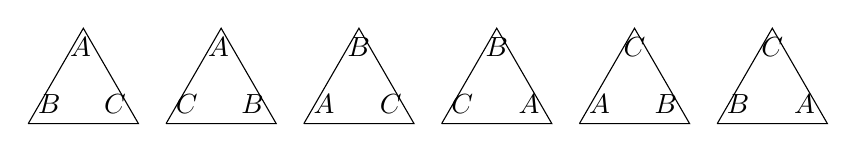
\begin{tikzpicture}[scale=0.7]
          \draw (-1,0)--(1,0)--(0,1.732)--(-1,0);
          \draw (-3.5,0)--(-1.5,0)--(-2.5,1.732)--(-3.5,0);
          \draw (-6,0)--(-4,0)--(-5,1.732)--(-6,0);
          \draw (4,0)--(6,0)--(5,1.732)--(4,0);
          \draw (1.5,0)--(3.5,0)--(2.5,1.732)--(1.5,0);
          \draw (6.5,0)--(8.5,0)--(7.5,1.732)--(6.5,0);
          \node[below] at (-5.05, 1.732) {$A$};
          \node[below] at (-2.55, 1.732) {$A$};
          \node[below] at (-0, 1.732) {$B$};
          \node[below] at (2.5, 1.732) {$B$};
          \node[below] at (5, 1.732) {$C$};
          \node[below] at (7.5, 1.732) {$C$};
          \node[above right] at (-6,0) {$B$};
          \node[above right] at (-3.5,0) {$C$};
          \node[above right] at (-1,0) {$A$};
          \node[above right] at (1.5,0) {$C$};
          \node[above right] at (4,0) {$A$};
          \node[above right] at (6.5,0) {$B$};
          \node[above left] at (-4.05,0) {$C$};
          \node[above left] at (-1.55,0) {$B$};
          \node[above left] at (0.95,0) {$C$};
          \node[above left] at (3.45,0) {$A$};
          \node[above left] at (5.95,0) {$B$};
          \node[above left] at (8.45,0) {$A$};
      \end{tikzpicture}
      \end{center}
      \item Dih$(4)$ is the group of all rotations and reflections that preserve the structure of the regular tetrahedron in $\mathbb{R}^{3}$. An incorrect, yet somewhat useful, way of visualizing this group is to imagine a square in $\mathbb{R}^{2}$. However, the points are not pairwise equidistant and therefore does not preserve symmetry between all points.
      \item Dih$(n)$ is similarly the group of all rotations and reflections that preserve the structure of a regular $(n-1)$-simplex in $\mathbb{R}^{n-1}$. 
    \end{enumerate}
  \end{example} 

  \begin{example}[Klein 4 Group]
    The \textbf{Klein 4-Group} can be described as the symmetry group of a non-square rectangle. With the three non-identity elements being horizontal reflection, vertical reflection, and 180-degree rotation. 

    \begin{figure}[H]
      \centering 
      \begin{tabular}{c|cccc}
        \hline
        $\cdot$ & $e$ & $a$ & $b$ & $c$ \\
        \hline
        $e$ & $e$ & $a$ & $b$ & $c$ \\
        $a$ & $a$ & $e$ & $c$ & $b$ \\
        $b$ & $b$ & $c$ & $e$ & $a$ \\
        $c$ & $c$ & $b$ & $a$ & $e$ \\
        \hline
      \end{tabular}
      \caption{Multiplication table for the Klein 4-group ($V_4$)} 
      \label{fig:klein4group}
    \end{figure}
  \end{example}

  \begin{example}[Groups of Order 4]
    There are only 2 groups of order 4. 
    \begin{figure}[H]
      \centering
      \begin{subfigure}[b]{0.48\textwidth}
        \centering
        \begin{tabular}{|c|c|c|c|c|}
          \hline
          $C_4$ & $e$ & $a$ & $a^2$ & $a^3$ \\
          \hline
          $e$ & $e$ & $a$ & $a^2$ & $a^3$ \\
          \hline
          $a$ & $a$ & $a^2$ & $a^3$ & $e$ \\
          \hline
          $a^2$ & $a^2$ & $a^3$ & $e$ & $a$ \\
          \hline
          $a^3$ & $a^3$ & $e$ & $a$ & $a^2$ \\
          \hline
        \end{tabular}
        \caption{Cyclic group $C_4$}
      \end{subfigure}
      \hfill 
      \begin{subfigure}[b]{0.48\textwidth}
        \centering
        \begin{tabular}{|c|c|c|c|c|}
          \hline
          $V$ & $e$ & $a$ & $b$ & $c$ \\
          \hline
          $e$ & $e$ & $a$ & $b$ & $c$ \\
          \hline
          $a$ & $a$ & $e$ & $c$ & $b$ \\
          \hline
          $b$ & $b$ & $c$ & $e$ & $a$ \\
          \hline
          $c$ & $c$ & $b$ & $a$ & $e$ \\
          \hline
        \end{tabular}
        \caption{Klein four-group $V$}
      \end{subfigure}
      \caption{Cayley tables for the two groups of order 4}
      \label{fig:order4groups}
    \end{figure} 
  \end{example}

\subsection{Symmetric and Alternating Groups}

  Notice that given any set $S$, we can define the set of all functions $f: S \rightarrow S$ as a monoid. What if we consider the set of all invertible functions? This by definition means bijective functions, and so consider this subset.  

  \begin{definition}[Symmetric/Transformation Group]
    Given a set $S$, the \textbf{transformation group}, or \textbf{symmetric group}, of $S$ is the group of all bijective maps from $S$ to itself. 
  \end{definition} 

  This exists for all sets $S$, and if $S$ is finite, we call it a \textbf{permutation group}, since the set of bijective transformations of it is a permutation of its elements. 

  \begin{definition}[Permutation Group]
    The \textbf{permutation group} is the set of all bijective transformations from any set $X$ to the same set, denoted either Sym$(X)$ or $S_n$. If $X = \{1, 2, 3 ,... , n\}$, known as the set of all permutations of $X$, with cardinality $n!$. 
  \end{definition}

  \begin{lemma}
    Every element in finite $S_{n}$ can be decomposed into a partition of cyclic rotations.
  \end{lemma}

  \begin{example}
    Listed.
    \begin{enumerate}
      \item $(1 2)$ is a mapping $1 \rightarrow 2,\; 2 \rightarrow 1$. 
      \item $(1 2 3)$ is a mapping $1\rightarrow 2,\; 2 \rightarrow 3,\; 3 \rightarrow 1$. 
      \item $(1 2 3) (4 5)$ is a mapping $1\rightarrow 2,\; 2 \rightarrow 3,\; 3 \rightarrow 1, \;4 \rightarrow 5, \;5 \rightarrow 4$. 
    \end{enumerate}
  \end{example}

  \begin{definition}
    The \textbf{conjugacy class} of $S_{n}$ correspond to the cycle structures of $S_{n}$. Two elements of $S_{n}$ are conjugate in $S_{n}$ if and only if they consist of the same number of disjoint cycles of the same lengths. 
  \end{definition} 

  \begin{example}
    \begin{enumerate}
      \item $(1 2 3) (4 5)$ is conjugate to $(1 4 3) (2 5)$.
      \item $(1 2) (4 5)$ is not conjugate to $(1 4 3) (2 5)$. 
    \end{enumerate}
  \end{example}

  \begin{theorem}[Transpositions]
    The set of all \textbf{transpositions} forms a generating set of $S_{n}$. 
  \end{theorem}

  \begin{definition}
    The \textbf{signature} of a permutation is a homomorphism
    \begin{equation}
      \text{sgn}: S_{n} \longrightarrow \{1, -1\}
    \end{equation}
  \end{definition}

  \begin{lemma}
    The signature of a permutation changes for every transposition that is applied to it. 
  \end{lemma}

  Now the reason that symmetric groups are nice is that we can embed a group into its symmetric group.  

  \begin{theorem}[Cayley's Theorem]
    Every group $G$ is isomorphic to a subgroup of its symmetric group. If $G$ is finite, then so is Sym$(G)$, so every finite group is a subgroup of $S_{n}$, for some $n$.
  \end{theorem}
  \begin{proof}
    Let $H =$ Sym$(G)$. We define the map
    \begin{equation}
      \phi: G \longrightarrow H
    \end{equation}
    by the following rule. For $a \in G$, map it to permutation $\sigma = \phi (a) \in H$ defined as $\sigma(g) = a g$ for all $g \in G$. Note that given an $a \in G$, $a g$ must also be in $G$, meaning that a corresponding $\sigma \in H$ exists. It is sufficient to prove that $\phi$ is an isomorphism onto its image. We first prove injectivity. Given $a \neq b \in G$, $\phi(a)=\sigma, \phi(b) = \tau$. Assume $\sigma = \tau \implies a = a e =  \sigma(e) = \tau (e) = b e = b \implies a = b$, a contradiction. We now check that $\phi(a b) = \phi(a) \phi(b)$. Given $g \in G, \phi(a) \phi(b) (g) = \phi(a) (bg) = a(bg)= (ab) g = \phi(ab) (g).$
  \end{proof}

  \begin{definition}[Alternating Group]
    The \textbf{alternating group} of order $n$ is the set of all \textbf{even permutations} (permutations that have signature $1$) of $\{1, 2, ..., n\}$. It is denoted $A_{n}$ or Alt$(n)$ and its cardinality is $\frac{1}{2} n!$. Note that the set of odd permutations do not form a group, since the composition of two odd permutations (each having signature $-1$ is an even permutation. 
  \end{definition}

  \begin{example}[Low Order Symmetric Groups]
    \begin{enumerate}
      \item $S_{0}$ is the set of all permutations on the \textbf{null set}. $S_{1}$ is the set of all permutations on the \textbf{singleton set}. Both sets have cardinality 1 and the element is \textbf{trivial}. Note that $S_{1} = A_{1}$. 
      \item $S_{2}$ is a cyclic, abelian group of order 2 consisting of the identity permutation and the transposition of two elements. 
      \item $S_{3}$ is the first cyclic, nonabelian group, with order 6.$S \simeq \text{Dih}(3)$, which can be seen as the group of rotations and reflections on the equilateral triangle, and the elements of $S_{3}$ equate to permuting the vertices on the triangle. 
    \end{enumerate}
  \end{example}

  In lecture, we talked about the number of all finite set is $e$. Since $n!$ is the order of permutation groups, i.e. the order of automorphism groups, we can sum their inverses over all $n \in \mathbb{N}$ to get $e$. 

\subsection{Group Actions} 

  \begin{definition}[Group Action]
    Let $G$ be a group, $X$ a set. Then, a (left) group action of $G$ on $X$ is a function: 
    \begin{equation}
      \varphi: G \times X \longrightarrow X, \; (g,x) \longmapsto \varphi(g,x)
    \end{equation}
    satisfying two axioms:
    \begin{enumerate}
      \item Identity. $\forall x \in X, \varphi(e, x) = x$. 
      \item Compatibility. $\forall g, h \in G \text{ and } \forall x \in X, \varphi(gh, x) = \varphi(g, \varphi(h, x))$.
    \end{enumerate}
    The group $G$ is said to \textbf{act on} $X$. $X$ is called a \textbf{G-set}. The two axioms, furthermore, imply that for every $g \in G$, the function that maps $x \in X$ to $ \varphi(g, x) \in X$ is a bijective map, since the inverse is the function mapping $x \mapsto \varphi(g^{-1}, x)$. \\
    $(g, x)$ can be interpreted as the element $g$ in the transformation group $G$ acting on an element $x$ in $X$.
  \end{definition}

  \begin{example}
    Isom$\,\mathbb{R}^{3}$ acts on $\mathbb{R}^{3}$ since every element $g \in$ Isom$\,\mathbb{R}^{3}$ acts on the entire space $\mathbb{R}^{3}$. 
  \end{example}

  \begin{example}
    $S_n$ acts on $\{1, 2, ..., n\}$by permuting its elements.
  \end{example}

  \begin{example}
    The GA$(V)$ acts transitively on the points of an affine space.
  \end{example}

  \textbf{Equivalent Interpretation of Group Actions}
  Note that this group action $G$ on space $X$ identifies a group homomorphism into the group of automorphisms of that space. Given an abstract group element $g \in G$, $\varphi(g, \cdot): X \longrightarrow X$ is defined accordingly, where $\varphi(g, \cdot) \in $ Aut$(X)$. So alternatively, we can interpret a group action as a homomorphism from $G$ to Aut$(X)$. 
  \begin{equation}
    \phi: G \longrightarrow \text{Aut}(X), \; g \mapsto \phi(g) = \varphi(g,\cdot)
  \end{equation}

  \begin{definition}[Representation]
    A group action on a finite-dimensional vector space $X$ is called a \textbf{representation} of that group. 
  \end{definition}


\section{Subgroups} 

  We have seen a few examples of subgroups, but we will heavily elaborate on here. We know that given a set, we can define an equivalence relation on it to get a quotient set. Now if we have a group, defining any such equivalence relation may not be compatible with the group structure. Therefore, it would be nice to have some principles in which we can construct such compatible equivalence classes, i.e. through a \textbf{congruence relation} that preserves the operations. 

\subsection{Cosets}

  Fortunately, we can do such a thing by taking a subgroup $H \subset G$ and ``shifting'' it to form the cosets of $G$, which are the equivalence classes. 
  
  \begin{definition}[Coset]
    Given a group $G$, $a \in G$, and subgroup $H$, 
    \begin{enumerate}
      \item A \textbf{left coset} is $a H \coloneqq \{a h \mid h \in H \}$. 
      \item A \textbf{right coset} is $H a \coloneqq \{h a \mid h \in H \}$. 
      \item When $G$ is abelian, the \textbf{coset} is denoted $a + H$. 
    \end{enumerate}
    With this, we can take arbitrary elements $a, b \in G$ and determine if they are in the same coset as such. Since $a \in aH$, $b \in aH$ iff $b = ah$ for some $h \in H$. Therefore, we have the equivalence relation. 
    \begin{equation}
      a \equiv b \pmod{H} \iff a = b h \text{ for some } h \in H
    \end{equation}
  \end{definition}
  \begin{proof}
    We show that this indeed forms an equivalence class. 
    \begin{enumerate}
      \item \textit{Reflexive}. $a \equiv a \pmod{H}$ since $e \in H \implies a = a e$. 
      \item \textit{Symmetric}. Let $a \equiv b \pmod{H}$. Then $a = bh$ for some $h \in H$, but since $H$ is a group, $h^{-1} \in H \implies a h^{-1} = b \implies b \equiv a \pmod{H}$. 
      \item \textit{Transitive}. Let $a \equiv b \pmod{H}$ and $b \equiv c \pmod{H}$. Then $a = bh$ and $b = ch^\prime$ for some $h, h^\prime \in H$. But then 
      \begin{equation}
        a = bh = (ch^\prime) h = c(h^\prime h)
      \end{equation}
      where $h^\prime h \in H$ due to closure. 
    \end{enumerate}
  \end{proof} 

  Note that a coset is \textit{not} a subgroup. It is only the case that $eH = H$ is a subgroup, but for $a \neq e$, $aH$ does not even contain the identity. We should think of a coset as a \textit{translation} of the subgroup $H$. 

  \begin{example}[Familiar Cosets]
    Here are some examples. Note that all it takes is to find \textit{some} subgroup, and the cosets will naturally pop up. 
    \begin{enumerate}
      \item Let $H = 2 \mathbb{Z} \subset (\mathbb{Z}, +)$ be the even integers. Then $0 + H$ and $1 + H$ are the even and odd integers, respectively. 
      \item Let $H = \{e, f\} \subset \Dih(3)$. Then 
      \begin{equation}
        H = \{e, f\}, rH = \{r, rf\}, r^2 H = \{r^2, r^2 f\} 
      \end{equation}
      are the cosets. 
    \end{enumerate}
  \end{example}

  With this partitioning scheme in mind, the following theorem on the order of such groups becomes very intuitive, and has a lot of consequences. 

  \begin{theorem}[Lagrange's Theorem]
    Let $G$ be a finite group and $H$ its subgroup. Then 
    \begin{equation}
      |G| = [G:H] |H|
    \end{equation}
    where $[G:H]$, called the \textbf{index of $H$}, is the number of cosets in $G$. Therefore, the order of a subgroup of a finite group divides the order of the group. 
  \end{theorem}
  \begin{proof}
    The union of the $[G:H]$ disjoint cosets is all of $G$. On the other hand, every $H$ is in one-to-one correspondence with each coset $aH$, so every coset has $|H|$ elements. Therefore, there are $[G:H] |H|$ elements altogether. 
  \end{proof}

  Therefore, Lagrange's theorem says that \textit{given} that you find a subgroup, the order of the subgroup must divide the order of $G$. However, that doesn't mean that such a subgroup may even exist. For example, there is a group of order 12 having no subgroup of order 6. 

  \begin{corollary}
    The order of any element of a finite group divides the order of the group. 
  \end{corollary}
  \begin{proof}
    Take any $a \in G$ and construct the cyclic subgroup $\langle a \rangle \subset G$. Then by Lagrange's theorem, $|a| = |\langle a \rangle|$ divides $|G|$. 
  \end{proof}

  \begin{corollary}
    Every finite group of a prime order is cyclic. 
  \end{corollary}
  \begin{proof}
    Let $a \in G$ be any element other than the identity $e$, and consider $\langle a \rangle \subset G$. The order must divide $|G|$ which is prime, so $|a| = 1$ or $|G|$. But $|a| \neq 1$ since we did not choose the identity, so $|a| = |G| \implies \langle a \rangle = G$. 
  \end{proof}

  \begin{corollary}
    If $|G| = n$, then for every $a \in G$ $a^n = e$. 
  \end{corollary}
  \begin{proof}
    Let $|a| = k$. Then $k \mid n$, and so $a^n = a^{kl} = (a^k)^l = e^l = e$. 
  \end{proof}

  \begin{corollary}[Fermant's Little Theorem]
    Let $p$ be a prime number. The multiplicative group $\mathbb{Z}_{p} \setminus \{0\}$ of the field $\mathbb{Z}_{p}$ is an abelian group of order $p-1 \implies g^{p-1} = 1$ for all $g \in \mathbb{Z}_{p} \setminus \{0\}$. So,
    \begin{equation}
      a^{p-1} \equiv 1 \iff a^{p} \equiv a \pmod{p}
    \end{equation}
  \end{corollary} 

  We can generalize this. 

  \begin{definition}[Euler's Totient Function]
    \textbf{Euler's Totient Function}, denoted $\varphi(n)$, consists of all the numbers less than or equal to $n$ that are coprime to $n$. 
  \end{definition}

  \begin{theorem}[Euler's Theorem]
    For any $n$, the order of the group $\mathbb{Z}_{n} \setminus \{0\}$ of invertible elements of the ring $\mathbb{Z}_{n}$ equals $\varphi(n)$, where $\varphi$ is Euler's totient function. In other words with $G = \mathbb{Z}_{n} \setminus \{0\}$, 
    \begin{equation}
      a^{\varphi(n)} \equiv 1 \pmod{n}, \; \text{ where $a$ is coprime to $n$}
    \end{equation}
  \end{theorem}

  \begin{example}
    In $\mathbb{Z}_{125} \setminus \{0\}$, $\varphi(125) = 125 - 25 = 100 \implies 2^{100} \equiv 1 \pmod{125}$
  \end{example}

\subsection{Normal Subgroups}

  By introducing cosets, we have successfully constructed an equivalence relation on $G$. This set of cosets is indeed a partition of $G$, but we would like to endow it with a group structure that respects that of $G$. That is, let $a, b \in G$ and its corresponding cosets be $aH, bH$. Then, we would like to define an operation $\cdot$ on the cosets such that 
  \begin{equation}
    (aH) \cdot (bH) \coloneqq (ab)H
  \end{equation} 
  That is, we would like to upgrade the equivalence relation to a \textit{congruence relation}. If we try to show that this is indeed a well-defined operation, we run into some trouble. Suppose $aH = a^\prime H$ and $bH = b^\prime H$. Then with our definition, we should be able to derive that $(aH)(bH) = (a^\prime H) (b^\prime H)$ through the equation 
  \begin{equation}
     (aH) (bH) = (ab)H = (a^\prime b^\prime) H = (a^\prime H) (b^\prime H) 
  \end{equation}
  We have $a^\prime = a h_1$, $b^\prime = b h_2$, and $a^\prime b^\prime = ab h$. Then, 
  \begin{align}
    (ab) H = (a^\prime b^\prime) H & \implies a^\prime b^\prime = abh \text{ for some } h \in H \\
                                   & \implies a h_1 b h_2 = abh \text{ for some } h_1, h_2, h \in H
  \end{align}
  But the final statement is not true in general. In an abelian group, we could just swap $h_1$ and $b$ to derive it completely, but perhaps there is a weaker condition on just the subgroup $H$ that allows us to ``swap'' the two. 

  \begin{definition}[Normal Subgroups]
    A subgroup $N \subset G$ is a \textbf{normal subgroup} iff the left cosets equal the right cosets. That is, $\forall g \in G, h \in H$. 
    \begin{equation}
      g^{-1} h g \in H
    \end{equation}
    We call $g^{-1} h g$ the \textbf{conjugate} of $h$ by $g$. 
  \end{definition} 

  As stated above, it is easy to see that every subgroup of an abelian group is normal. In fact, we can do better. 

  \begin{lemma} 
    A subgroup $H \subset G$ is normal if and only if there exists a group homomorphism $\phi: G \rightarrow G^\prime$ with $\ker{\phi} = H$. 
  \end{lemma}
  \begin{proof}
    We prove bidirectionally. 
    \begin{enumerate}
      \item $(\rightarrow)$. Since $H$ is normal, we can form the quotient group $G/H$. Let $\phi: G \rightarrow G/H$ be defined $\phi(a) = aH$. Then, 
      \begin{align}
        \ker{\phi} = \phi^{-1}(eH) & = \{a \in G \mid aH = eH = H \} \\
                                   & = \{a \in G \mid a \in H \}
      \end{align}
      Therefore, $\phi$ is a homomorphism because $\phi(ab) = abH = (aH)(bH)$. 
    \end{enumerate}
  \end{proof}

  \begin{example}[Normal Subgroups]
    
  \end{example}

  \begin{example}[Subgroups that are Not Normal]
    
  \end{example}

\subsection{Quotient Groups}

  Now that we know about normal subgroups, this allows us to endow on the quotient set a group structure. 

  \begin{definition}[Quotient Group]
    Given a group $G$ and a normal subgroup $H$, the \textbf{quotient group} $G/H$ is the set of left cosets $aH$ with 
    \begin{enumerate}
      \item the operation $(aH) \cdot (bH) \coloneqq (ab)H$ 
      \item the identity element $eH$. 
      \item inverses $(aH)^{-1}) = (a^{-1})H$. 
    \end{enumerate}
    and order $|G/H| = |G| / |H|$.  
  \end{definition}
  \begin{proof}
    It suffices to check that multiplication is well defined. Suppose as above that $aH = a^\prime H$ and $bH = b^\prime H$. Then $a^\prime = ah$ and $b^\prime = bk$ for some $h, k \in H$. Since $H$ is normal, $b^{-1} h b = h^\prime$ for some $h^\prime \in H$. Therefore, 
    \begin{equation}
      a^\prime b^\prime = (ah) (bk) = a(hb) k = (ab h^\prime) k = (ab)(h^\prime k) \in (ab) H
    \end{equation}
    and so $(ab)H = (a^\prime b^\prime)H$. 
  \end{proof}

  \begin{theorem}[Quotient Maps are Homomorphisms]
    The map $\pi: G \rightarrow G/H$ is a group homomorphism, and the \textbf{quotient group} is the set of left cosets with 
  \end{theorem}
  \begin{proof}
    
  \end{proof} 

  \begin{theorem}[Fundamental Group Homomorphism Theorem]
    Let $f: G \to G^\prime$ be a surjective homomorphism. Then $G/{\ker{f}} \simeq G^\prime$.\footnote{Note that if $f$ is not surjective, we can just have it be surjective by restricting $G^\prime$ to be the image of $f$. }

    \begin{figure}[H]
      \centering 
      \begin{tikzcd}
        G \arrow[r, "f"] \arrow[d, "p"] & G' \\
        G/\ker{f} \arrow[ur, "\bar{f}"'] &
      \end{tikzcd}
      \caption{Given $f$ and the projection map $p: G \to G/{\ker{f}}$, this induces an isomorphism $\bar{f}$ such that $f = \bar{f} \circ p$.} 
      \label{fig:group_fund_homo_theorem}
    \end{figure}
  \end{theorem}

\subsection{Orbits and Stabilizers}

  \begin{definition}[Orbits]
    Let $G$ be a transformation group on set $X$. Points $x, y \in X$ are equivalent with respect to $G$ if there exists an element $g \in G$ such that $y = g x$. This has already been defined through the equivalence of figures before. This relation splits $X$ into equivalence classes, called \textbf{orbits}. Note that cosets are the equivalence classes of the transformation group $G$; oribits are those of $X$. We denote it as
    \begin{equation}
      Gx \equiv \{ g x \;|\;g \in G \}
    \end{equation}
  \end{definition}

  By definition, transitive transformation groups have only one orbit.

  \begin{definition}
    The subgroup $G_{x} \subset G$, where $G_{x} \equiv \{ g \in G | g x = x\}$ is called the \textbf{stabilizer} of $x$.
  \end{definition}

  \begin{example}
    The orbits of $O(2)$ are concentric circles around the origin, as well as the origin itself. The stabilizer of $0$ is the entire $O(2)$.
  \end{example}

  \begin{example}
    The group $S_n$ is transitive on the set $\{1, 2, ..., n\}$. The stabilizer of $k, (1 \leq k \leq n)$ is the subgroup $H_{k} \simeq S_{n-1}$, where $H_k$ is the permutation group that does not move $k$ at all. 
  \end{example}

  \begin{theorem}
    There exists a 1-to-1 injective correspondence between an orbit $G_x$ and the set $G / G_{x}$ of cosets, which maps a point $y = g x \in G x $ to the coset $g G_x$. 
  \end{theorem}

  \begin{corollary}
    If $G$ is a finite group, then 
    \begin{equation}
      |G| = |G_x| |G x|
    \end{equation}
    In fact, there exists a precise relation between the stabilizers of points of the same orbit, regardless of $G$ being finite or infinite: 
    \begin{equation}
      G_{g x} = g G_{x} g^{-1}
    \end{equation}
  \end{corollary}

\subsection{Centralizers and Normalizers} 

\subsection{Lattice of Subgroups} 


\section{Group Actions} 

\subsection{Sylow Theorems}

\subsection{Exercises}


\section{Classification of Groups} 

\subsection{Direct Products}

  \begin{definition}[Direct Product]
    The \textbf{direct product} of two groups $(G, \cdot)$ and $(H, \ast)$ is the set 
    \begin{equation}
      G \times H \equiv \{ (g, h) \mid g \in G, h \in H \}
    \end{equation} 
    equipped with the operation 
    \begin{equation}
      (g_1, h_1) \cdot (g_2, h_2) \coloneqq (g_1 \cdot g_2, h_1 \ast h_2)
    \end{equation}
  \end{definition}
  \begin{proof}
    It is pretty trivial to see that this is a group. 
  \end{proof}

  \begin{example}[General Affine Group]
    The \textbf{general affine group} is defined 
    \begin{equation}
      \GA(V) \equiv \Tran(V) \times \GL(V)
    \end{equation}
  \end{example}

  \begin{example}[Galileo Group]
    The \textbf{Galileo Group} is the transformation group of spacetime symmetries that are used to transform between two reference frames which differ only by constant relative motion within the constructs of Newtonian physics. It is denoted 
    \begin{equation}
      \Tran \mathbb{R}^{4} \times H \times \O(3)
    \end{equation}
    where $H$ is the group of transformations of the form 
    \begin{equation}
      (x, y, z, t) \mapsto (x+at, y+bt, z+ct, t)
    \end{equation}
  \end{example}

  \begin{example}[Poincaré Group]
    The \textbf{Poincaré Group} is the symmetry group of spacetime within the principles of relativistic mechanics, denoted
    \begin{equation}
      G = \Tran \mathbb{R}^{4} \times \O_{3,1}
    \end{equation}
    where $\O_{3,1}$ is the group of linear transformations preserving the polynomial 
    \begin{equation}
      x^{2} + y^{2} + z^{2} - t^{2}
    \end{equation}
  \end{example} 

\subsection{Semidirect Products} 

\subsection{Classification of Finite Abelian Groups} 

  \begin{theorem}[Groups of Order 1, 2, 3]
    We have the following. 
    \begin{enumerate}
      \item There is only one group of order 1. 
        \begin{equation}
          Z_1 \simeq S_1 \simeq A_2
        \end{equation}

      \item There is only one group of order 2. 
        \begin{equation}
          Z_2 \simeq S_2 \simeq D_2
        \end{equation}

      \item There is only one group of order 3. 
        \begin{equation}
          Z_3 = A_3
        \end{equation}
    \end{enumerate}
  \end{theorem}

  \begin{theorem}[Groups of Order 4]
    There are two groups of order 4. 
    \begin{equation}
      Z_4, \qquad Z_2^2 \simeq D_4
    \end{equation}
  \end{theorem}

\subsection{Group Extensions}

\subsection{Classification of Simple Groups of Small Order}

  \begin{theorem}[Classification of Simple Groups of Small Order]
    The following are the only groups of order $n$. You can notice that it is dominated by direct products of cyclic groups, since they exist for every order, while the other types increase in order very fast.   

    \begin{figure}[H]
      \centering
      \begin{tabular}{|c|l|l|}
      \hline
      $n$ & \textbf{Abelian Groups} & \textbf{Non-Abelian Groups} \\
      \hline
      1 & $\{e\}$ (trivial group) & None \\
      \hline
      2 & $\mathbb{Z}_2 = S_2 = \text{Dih}(1)$ & None \\
      \hline
      3 & $\mathbb{Z}_3 = A_3$ & None \\
      \hline
      4 & $\mathbb{Z}_4$, $\mathbb{Z}_2 \times \mathbb{Z}_2 = \text{Dih}(2)$ & None \\
      \hline
      5 & $\mathbb{Z}_5$ & None \\
      \hline
      6 & $\mathbb{Z}_6 = \mathbb{Z}_3 \times \mathbb{Z}_2$ & $S_3 = \text{Dih}(3)$ \\
      \hline
      7 & $\mathbb{Z}_7$ & None \\
      \hline
      8 & $\mathbb{Z}_8$, $\mathbb{Z}_4 \times \mathbb{Z}_2$, $\mathbb{Z}_2 \times \mathbb{Z}_2 \times \mathbb{Z}_2$ & $D_4 = \text{Dih}(4)$, $Q_8$ (quaternion) \\
      \hline
      9 & $\mathbb{Z}_9$, $\mathbb{Z}_3 \times \mathbb{Z}_3$ & None \\
      \hline
      10 & $\mathbb{Z}_{10} = \mathbb{Z}_5 \times \mathbb{Z}_2$ & $D_5 = \text{Dih}(5)$ \\
      \hline
      11 & $\mathbb{Z}_{11}$ & None \\
      \hline
      12 & $\mathbb{Z}_{12} = \mathbb{Z}_4 \times \mathbb{Z}_3$, $\mathbb{Z}_6 \times \mathbb{Z}_2$, $\mathbb{Z}_2 \times \mathbb{Z}_2 \times \mathbb{Z}_3$ & $A_4$, $D_6 = \text{Dih}(6)$, $\mathbb{Z}_3 \rtimes \mathbb{Z}_4$ (dicyclic) \\
      \hline
      \end{tabular}
      \caption{Classification of groups up to order 12.}
      \label{tab:groups_up_to_order_10}
    \end{figure}
  \end{theorem}

\subsection{Exercises}

\section{Ring-Like Structures} 

  We have extensively talked about groups, and now we look at an algebraic structure called a ring that has two operations. As we introduce rings, we will use the integers as the primary structure to demonstrate our theorems, along with the ring of continuous functions and the ring of matrices. 

  \begin{definition}[Ring]
    A \textbf{ring} is a set $(R, +, \times)$ equipped with two operations, called addition and multiplication. It has properties: 
    \begin{enumerate}
      \item $R$ is an abelian group with respect to $+$, where we denote the additive identity as $0$ and the additive inverse of $x$ as $-x$. 
      \item $R$ is a monoid with respect to $\times$, where we denote the multiplicative identity as $1$, also known as the \textbf{unity}. 
      \item $\times$ is both left and right distributive with respect to addition $+$
      \begin{align}
        a \times (b + c) & = a\times b + a\times c \\ 
        (a + b) \times c & = a\times c + b\times c 
      \end{align}
      for all $a, b, c \in \mathbb{R}$. 
    \end{enumerate} 
    If $\times$ is associative, $R$ is called an \textbf{associative ring}, and if $\times$ is commutative, $R$ is called a \textbf{commutative ring}. 
  \end{definition}

  In fact, in some cases the existence of the multiplicative identity is not even assumed, though we will do it here.\footnote{If a multiplicative identity is not assumed, then this is called an \textit{rng}, or a \textit{rung}.} Since a ring is a group with respect to addition, we know from \ref{thm:unique_add_inverse} that additive inverses are unique. However, we can say a little more with rings because of the distributive property. 

  \begin{lemma}[Additive Inverses] 
    For any $a \in R$, $-a = -1 \times a$. 
  \end{lemma}
  \begin{proof}
    We can see that 
    \begin{align}
      -1 + 1 = 0 & \implies (-1 + 1) \times a = 0 \times a \\
                 & \implies -1 \times a + 1 \times a = 0 \\
                 & \implies -1 \times a + a = 0 
    \end{align}
    and therefore by definition $-1 \times a$ must be the additive inverse. 
  \end{proof} 

  It helps to see some familiar examples of rings first before examining their properties. 

  \begin{example}[Integers, Rationals, Reals, Complexes]
    $(\mathbb{Z}, +, \times)$, $(\mathbb{Q}, +, \times)$, $(\mathbb{R}, +, \times)$, $(\mathbb{C}, +, \times)$ are all commutative rings, with additive and multiplicative identities $0$ and $1$. 
  \end{example}

  \begin{example}[Matrices]
    The set of matrices $\mathbb{R}^{n \times n}$\footnote{really over any field and even more generally a ring $R$} forms a noncommutative ring under matrix addition $+$ and multiplication $\times$. It has the additive and multiplicative identities $0$ and $I_{n}$. This forms a non-commutative ring for $n > 1$, even when $R$ is commutative.
  \end{example}

  \begin{example}[Continuous Functions]
    The set of all continuous functions $f: \mathbb{R} \rightarrow \mathbb{R}$ is a ring under point-wise addition and multiplication. 
  \end{example}

  \begin{example}[Power Set]
    Given a set $X$, $(2^X, \bigtriangleup, \cap)$ is a commutative associative ring with respect to the operations of symmetric difference $M \bigtriangleup N \coloneqq (M \setminus N) \cup (N \setminus M)$ and intersection. The additive identity is $\emptyset$ and the multiplicative identity is $X$. We can clearly see that both operations are commutative and $\cap$ is associative. 
    \begin{align*}
      M \bigtriangleup N & = (M \setminus N) \cup (N \setminus M) \equiv N \bigtriangleup M \\
      M \cap N & = N \cap M \\
      M \cap N \cap P & = (M \cap N) \cap P = M \cap (N \cap P)
    \end{align*}
  \end{example}

  Next, just like how we did for groups, we can talk about subrings. 

  \begin{definition}[Subring]
    Given ring $(R, +, \times)$ a \textbf{subring} $(S, +, \times)$ is a ring such that $S \subset R$. $S$ is called a \textbf{proper subring} if $S \subsetneq R$. 
  \end{definition}

  \begin{theorem}[Intersections of Subrings is a Subring]
    If $S_1, S_2$ are subrings of $R$, then $S_1 \cap S_2$ is a subring. 
  \end{theorem}

  Finally, we will mention a product ring. 

  \begin{definition}[Direct Product of Rings]
    Given rings $(R, +_R, \times_R)$ and $(S, +_S, \times_S)$, the direct product of the rings is the set $R \times S$ with the operations 
    \begin{enumerate}
      \item $(r_1, s_1) + (r_2, s_2) \coloneqq (r_1 +_R r_2, s_1 +_S s_2)$. 
      \item $(r_1, s_1) \times (r_2, s_2) \coloneqq (r_1 \times_R r_2, s_1 \times_S s_2)$. 
    \end{enumerate}
  \end{definition}
  \begin{proof}
    The proof is standard. 
  \end{proof}

\subsection{Ring Homomorphisms}

  So far, we have talked about many properties of rings but have not thoroughly gone over their classification. This is what we will do in this section, just like how we have classified groups. It turns out that classifying rings is significantly harder to do so, so we will talk about some low-order finite rings and provide some examples of isomorphisms between more complex rings. 

  \begin{definition}[Ring Homomorphism, Isomorphism]
    A \textbf{ring homomorphism} $f: R \rightarrow S$ is a function that satisfies for all $a, b \in R$
    \begin{enumerate}
      \item $f(a + b) = f(a) + f(b)$
      \item $f(ab) = f(a) f(b)$ 
      \item $f(1_R) = 1_S$\footnote{The reason we need this third is that while $f$ is a group homomorphism with respect to $+$, it automatically follows that $f(0) = 0$. However $f$ is only a monoid homomorphism w.r.t. $\times$, and so we need this extra constraint. }
    \end{enumerate}
    for all $a, b \in R$.\footnote{Note that the first is equivalent to it being a group homomorphism between $(R, +)$ and $(S, +)$. The second property may look like it is a group homomorphism between $(R, \times)$ and $(S, \times)$, but remember that neither are groups and it just states that closure distributes. Combined with the fact that the multiplicative identity matches, $f$ is really a homomorphism of \textit{monoids}. } Furthermore, 
    \begin{enumerate}
      \item A \textbf{ring isomorphism} is a bijective ring homomorphism, and we call rings $R$ and $S$ isomorphic, denoted $R \simeq S$ if there exists an isomorphism between them. 
      \item A \textbf{ring endomorphism} is a ring homomorphism onto itself. 
      \item A \textbf{ring automorphism} is an isomorphism from a ring to itself. 
    \end{enumerate}
  \end{definition} 

  \begin{example}[Homomorphisms of Rings]
    We provide some simple examples of ring homomorphisms. 
    \begin{enumerate}
      \item The identity map $\iota : R \to R$ is a ring homomorphism. 
      \item If $R \subset S$ as rings, then the canonical injection map $\iota: R \to S$ is a ring homomorphism. 
      \item Complex conjugation $z \in \mathbb{C} \mapsto \bar{z} \in \mathbb{C}$ is a ring automorphism. 
    \end{enumerate}
  \end{example} 

  \begin{definition}[Kernel]
    The \textbf{kernel} of a ring homomorphism $f: R \rightarrow S$ is the preimage of $0 \in S$.\footnote{Note that this is the additive identity, not the multiplicative identity. We must specify which identity, unlike a group which has just one identity.}
  \end{definition}

  \begin{lemma}[Images and Kernels of Ring Homomorphisms]
    If $f: R \rightarrow S$ is a ring homomorphism, then 
    \begin{enumerate}
      \item $\im{f}$ is a subring of $S$. 
      \item $f$ is injective iff $\ker{f} = \{0\}$. 
    \end{enumerate}
  \end{lemma}
  \begin{proof}
    For the first claim, let $x, y, z \in \im{f}$. Then $x = f(a), y = f(b), z = f(c)$ for some $a, b \in R$. 
    \begin{enumerate}
      \item \textit{Closed under Addition}. $x + y = f(a) + f(b) = f(a + b) \in \im{f}$. 
      \item \textit{Associative under Addition}. $(x + y) + z = f(a + b) + f(c) = f((a + b) + c) = f(a + (b + c)) = f(a) + f(b + c) = x + (y + z)$
      \item \textit{Additive Identity}. $f(0) = 0$
      \item \textit{Additive Inverses}. We claim that $x^{-1} = f(a)^{-1} = f(a^{-1})$. Indeed, we have $f(a) f(a^{-1}) = f(a a^{-1}) = f(1) = 1$. 
      \item \textit{Closed under Multiplication}. $xy = f(a) f(b) = f(ab) \in \im{f}$. 
      \item \textit{Multiplicative Identity}. $f(1) = 1$. 
    \end{enumerate}
    For the second claim, we prove bidirectionally. 
    \begin{enumerate}
      \item $(\rightarrow)$. Let $\ker{f} \neq \{0\}$ and call its nonzero element $k$. Then, $f(a + k) = f(a) + f(k) = f(a) + 0 = f(a)$, and so $f(a) = f(a + k)$, which means $f$ is not injective. 
      \item $(\leftarrow)$. Assume that $f$ is not injective. Then there exists $a, b \in R$ s.t. $f(a) = f(b)$. This means that $0 = f(a) - f(b) = f(a - b)$, and so $a - b \in \ker{f}$. 
    \end{enumerate}
  \end{proof}

  Note that $\ker{f}$ is \textit{not} a subring, and we can quickly verify this by noticing that the identity element does not necessarily have to be in the kernel. However, we will see later that this is a specific instance of a more general structure called an \textit{ideal}. 

  \begin{theorem}[Compositions of Ring Homomorphisms]
    Compositions of ring homomorphisms are ring homomorphisms. 
  \end{theorem} 
  \begin{proof}
    Let $R \xrightarrow{f} S \xrightarrow{g} T$ be two ring homomorphisms. We can see that 
    \begin{enumerate}
      \item $(g \circ f)(a + b) = g( f(a) + f(b)) = g(f(a)) + g(f(b))$. 
      \item $g(f(ab)) = g(f(a) f(b)) = g(f(a)) + g(f(b))$ 
      \item $g(f(1_R)) = g(1_S) = 1_T$
    \end{enumerate}
  \end{proof}

  Now let's focus a bit more on ring isomorphisms. The following should be intuitive. 

  \begin{lemma}[Properties of Ring Isomorphisms]
    If $f: R \to S$ is a ring isomorphism, then $f^{-1}$ is a ring isomorphism. 
  \end{lemma} 
  \begin{proof}
    Since $f$ is a bijection, $f^{-1}$ is well defined and is a bijection. Now let $x, y \in S$, which implies that $x = f(a), y = f(b)$ for a unique $a, b \in R$. Now we see that $f^{-1}$ satisfies the 3 properties of a ring homomorphism. 
    \begin{enumerate}
      \item $f^{-1} (x + y) = f^{-1} (f(a) + f(b)) = f^{-1}(f(a + b)) = a + b = f^{-1}(a) + f^{-1} (b)$. 
      \item $f^{-1} (x y) = f^{-1} (f(a) f(b)) = f^{-1}(f(a b)) = a b = f^{-1}(a) f^{-1} (b)$. 
      \item $f^{-1}(1_S) = 1_R$. 
    \end{enumerate}
    Therefore, as a bijective ring homomorphism $f^{-1}$ is also a ring isomorphism. 
  \end{proof}

\subsection{Commutative Rings} 

  Note that we do not assume that there exists multiplicative inverses in a ring. However, there may be some elements for which multiplicative inverses do exist, i.e. $a, b \in R$ where $ab = 1$.  

  \begin{definition}[Unit]
    A \textbf{unit} of a ring $R$ is an element $u \in R$ that has a multiplicative inverse in $R$. That is, there exists a $v \in R$ s.t. $uv = vu = 1$. 
  \end{definition}

  Another property that we would desire is some sort of decomposition of ring elements as other ring elements. More specifically, the existence of elements $a, b$ such that $ab = 0$ will be of particular interest to us. 

  \begin{definition}[Left, Right Divisor]
    Let $a, b, r \in R$ a ring. 
    \begin{enumerate}
      \item If $ab = r$, then $a$ is said to be a \textbf{left divisor} of $r$ and $b$ a \textbf{right divisor} of $r$. 

      \item $a$ is said to be a left divisor of $r$ if it is a left divisor and a right divisor of $r$: $ax = ya = r$, but $x$ does not necessarily equal $y$. 

      \item If $ab = 0$, then $a$ and $b$ are said to be a \textbf{left zero divisor} and \textbf{right zero divisor}, respectively. 
    \end{enumerate}
    If $R$ is commutative, then we just call $a$ a \textbf{divisor} of $r$ or a \textbf{zero divisor}.\footnote{$a$ is a right divisor of $b \iff \exists x (xa = b) \iff \exists x (ax = b) \iff a$ is a left divisor. } 
  \end{definition}

  It turns out that the existence of units and zero divisors classify rings into subcategories, which we will elaborate on. That is, we will start with the most general theory on rings, and then shrink down into subcategories of rings. 

  \begin{figure}[H]
    \centering 
    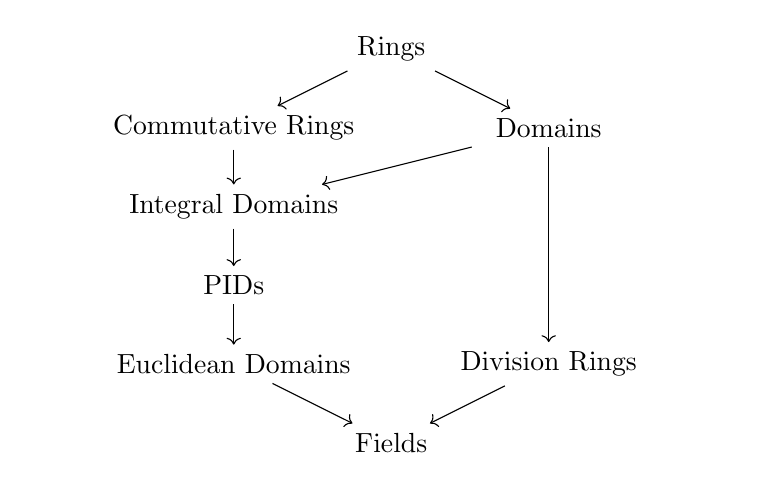
\begin{tikzpicture}[
        node distance=2cm,
        box/.style={
            text width=5cm,
            align=center
        }
    ]
        % Nodes for ring types
        \node[box] (rings) at (0,0) {Rings};
        \node[box] (comm) at (-2,-1) {Commutative Rings};
        \node[box] (domains) at (2,-1) {Domains};
        \node[box] (int) at (-2,-2) {Integral Domains};
        \node[box] (divring) at (2,-4) {Division Rings};
        \node[box] (pid) at (-2,-3) {PIDs};
        \node[box] (euc) at (-2,-4) {Euclidean Domains};
        \node[box] (fields) at (0,-5) {Fields};
        
        % Left path arrows
        \draw[->] (rings) -- (comm);
        \draw[->] (comm) -- (int);
        \draw[->] (int) -- (pid);
        \draw[->] (pid) -- (euc);
        \draw[->] (euc) -- (fields);
        \draw[->] (divring) -- (fields);
        
        % Right path arrows
        \draw[->] (rings) -- (domains);
        \draw[->] (domains) -- (int);
        \draw[->] (domains) -- (divring);
    \end{tikzpicture}
    \caption{Basic hierarchy of rings.} 
    \label{fig:ring_hierarchy}
  \end{figure} 
  
  Remember that for commutative rings, distinguishing left and right divisors are meaningless, and so we can talk about just \textit{divisors}. Almost all rings that we will deal with are commutative, so let's try to find some properties of commutative rings.  

  \begin{definition}[Prime and Compositive Elements]
    In a commutative ring $R$, an element $p \in R$ is said to be \textbf{prime} if it is not $0$, not a unit, and has only divisors $1$ and $p$. 
  \end{definition}

  \begin{lemma}[Euclid's Lemma]
    If $p$ is prime, then $p \mid ab \implies p \mid a$ or $p \mid b$.  
  \end{lemma}
  \begin{proof}
    We prove the contrapositive. Assume that prime $p$ does not divide $a$ nor $b$. We wish to show that $p \nmid ab$. Now for the sake of contradiction, assume that $p \mid ab$. Then $ab = pd$ for some $d \in R$. 
  \end{proof}

  \begin{lemma}[Divisibility of Linear Combinations of Rings Elements]
    Let $R$ be a commutative ring and $a, b, d \in R$. If $d \mid a$ and $d \mid b$, then $d \mid (ma + nb)$ for any $m, n \in R$. 
  \end{lemma} 

  \begin{definition}[Greatest Common Divisor]
    The \textbf{greatest common divisor} of elements $a$ and $b$, denoted $\gcd(a, b)$ of an commutative ring $R$ is a common divisor of $a$ and $b$ divisible by all their common divisors. That is, it is the element $d \in R$ satisfying 
    \begin{enumerate}
      \item $d \mid a$ and $d \mid b$ 
      \item if $k \mid a$ and $k \mid b$, then $k \mid d$. 
    \end{enumerate}
    If $\mathrm{gcd}(a, b) = 1$, then $a$ and $b$ are said to be \textbf{relatively prime}. 
  \end{definition} 

  Note that in an arbitrary commutative ring, the gcd of two elements always exists since we can at least identify $1$, but there may not be a \textit{unique} gcd. 

\subsection{Domains}

  We can see that domains behave similarly to the integers, but with the missing property that $\times$ is commutative. This motivates the following definition of an integral domain, which can be seen as a generalization of the integers. 

  \begin{definition}[Domain, Integral Domain]
    A ring $R$ with no zero divisors for every element is called a \textbf{domain}. An \textbf{integral domain} is a commutative domain $R$.\footnote{Almost always, we work with integral domains so we will default to this.} 
  \end{definition} 

  \begin{example}[Domains vs Integral Domains]
    We show some examples of domains and integral domains. 
    \begin{enumerate}
      \item $(\mathbb{Z}, +, \times)$ is an integral domain
      \item $(\mathbb{Q}, +, \times)$ is an integral domain. 
      \item $(\mathbb{R}, +, \times)$ is an integral domain. 
      \item Quaternions $\mathbb{H}$ are not commutative but are a domain. 
    \end{enumerate}
  \end{example} 

  \begin{example}[Non-Domains]
    Here are some examples of non-domains. 
    \begin{enumerate}
      \item The ring of $n \times n$ matrices over any nonzero ring when $ n \geq 2$ is not a domain. Given matrices $A, B$, if the image of $B$ is in the kernel of $A$, then $A B = 0$.
      \item The ring of continuous functions on the interval is not a domain. To see why, notice that given the piecewise functions 
      \begin{equation}
        f (x) = \begin{cases}
        1 - 2x & x \in [0, \frac{1}{2}] \\
        0 & x \in [\frac{1}{2}, 1] 
        \end{cases}, \; \;\;g (x) = \begin{cases}
        0 & x \in [0, \frac{1}{2}] \\
        2x - 1 & x \in [\frac{1}{2}, 1] 
        \end{cases}
      \end{equation}
      $f, g \neq 0$, but $f g = g f = 0$. 

      \item A product of two nonzero commutative rings with unity $R \times S$ is not an integral domain since $(1,0) \cdot (0, 1) = (0, 0) \in R \times S$. 
    \end{enumerate}
  \end{example}

  Here is an alternative equivalent characterization of an integral domain. 

  \begin{definition}[Regular Elements]
     An element $r$ of a ring $R$ is \textbf{regular} if the mapping 
     \begin{equation}
       \rho: R \longrightarrow R, \qquad x \mapsto x r
     \end{equation}
    is injective for all $x \in R$. 
  \end{definition}

  \begin{theorem}[Integral Domains w.r.t. Regularity]
    An integral domain is a commutative associative ring where every element is regular. 
  \end{theorem} 

  Finally, we talk about the properties of integral domains. Namely, that the characteristic must be prime and that gcd's---while not yet unique---are now guaranteed to be \textit{associated}. 

  \begin{theorem}[Characteristic of an Integral Domain]
    The characteristic of an integral domain is either $0$ or a prime number. 
  \end{theorem}

  While we have shown that gcd's exist in commutative rings, we can say a bit more when working in Euclidean domains. 

  \begin{definition}[Associate Elements]
    Elements $a$ and $b$ are \textbf{associated}, denoted $a \sim b$ if either of the following equivalent conditions holds
    \begin{enumerate}
        \item $a | b \text{ and } b | a$
        \item $a = c b, \text{ where } c$ is invertible
    \end{enumerate}
    The two conditions are equivalent because $c$ and $c^{-1}$ are both in $A$. 
  \end{definition} 

  \begin{theorem}[GCD's in a Euclidean Domain]
    Any two distinct gcd's of $a, b$ in a Euclidean domain must be associate elements. 
  \end{theorem}

\subsection{Ideals}

  Now assuming that $R$ and $S$ are commutative rings, let's consider a special sort of subset of a commutative ring. Consider the kernel of the ring homomorphism. We can see that if $a, b \in \ker(f)$, then $f(a + b) = f(a) + f(b) = 0 + 0 = 0$, and so $\ker(f)$ is closed under addition. Furthermore, $a \in \ker(f)$ and \textit{any} $b \in R$ gives $f(ab) = f(a) f(b) = 0 f(b) = 0$, and so multiplying any element in the kernel by an arbitrary element in the rings keeps it in the kernel. We would like to generalize these properties into an \textit{ideal}. 

  \begin{definition}[Ideals]
    For a commutative ring $(R,+, \times)$, a \textbf{two-sided ideal}---or \textbf{ideal}---is a subset $I \subset R$ satisfying 
    \begin{enumerate}
      \item $(I, +)$ is a subgroup of $(R, +)$. 
      \item $a \in I, r \in R \implies ra = ar \in I$.\footnote{Note that this property and closure under addition actually implies that it is a subgroup. Since we can see that $-1 \in R$ and $a \in I$ implies $-1 \cdot a = -a \in I$.}
    \end{enumerate}
    If $R$ is not necessarily commutative, then we $ra \neq ar$ in general, so we may distinguish between left and right ideals. 
  \end{definition}

  Therefore, we can see that it is an abelian group under $+$ and closed under $\times$. However, it is not guaranteed to have a multiplicative identity, which is why we can interpret $I$ as a ring without a multiplicative identity, also known as a \textit{rung}. 

  This seems like a pretty abstract definition, but a good intuition to have---though not completely accurate---is that ideals are a collection of \textit{multiples} of a certain element.\footnote{This is actually more accurate for a principal ideal.} They are analogous to normal subgroups, which were used to induce a congruence relation on a group to get its quotient. Ideals play a similar role. 

  \begin{example}[Multiples of Elements Are an Ideal]
    We give 2 ideals: 
    \begin{enumerate}
      \item The set of even integers $2 \mathbb{Z}$ is an ideal in the ring $\mathbb{Z}$, since the sum of any even integers is even and the product of any even integer with an integer is an even integer. However, the odd integers do not form an ideal. 
      \item The set of all polynomials with real coefficients which are divisible by the polynomial $x^2 + 1$ is an ideal in the ring of all polynomials. 
    \end{enumerate}
  \end{example}

  Let's talk about a few more properties of ideals, namely their construction and behavior under set theoretic operations. 

  \begin{theorem}[Sum and Intersection of Ideals are Ideals] 
    \label{thm:sum_int_ideals}
    Given two ideals $I, J \subset R$, 
    \begin{enumerate}
      \item $I \cap J$ is an ideal. 
      \item $I + J \coloneqq \{i + j \mid i \in I, j \in J\}$ is an ideal. 
    \end{enumerate}
  \end{theorem}
  \begin{proof}
    Listed. 
    \begin{enumerate}
      \item $I \cap J$ is an ideal. Given $a, b \in I \cap J$, then $a, b \in I \implies a + b \in I$, and $a, b \in J \implies a + b \in J$. So $a + b \in I \cap J$. Furthermore, for every $r \in R$, $a \in I \implies r a \in I$ and $a \in J \implies r a \in J$, so $a \in I \cap J \implies ra \in I \cap J$. 

      \item $I + J$ is an ideal. Given $x, y \in I + J$, then $x = a_x + b_x$ and $y = a_y + b_y$ for $a_x, a_y \in I, b_x, b_y \in J$. So 
      \begin{equation}
        x + y = (a_x + b_x) + (a_y + b_y) = (a_x + a_y) + (b_x + b_y)
      \end{equation}
      where $a_x + a_y \in I, b_x + b_y \in J$ by definition of an ideal, and so $x + y \in I + J$. Noe let $x = a_x + b_x \in I + J$. Then given $r \in R$,
      \begin{equation}
        rx = r(a_x + b_x) = r a_x + r b_x
      \end{equation}
      where $r a_x \in I$ and $r b_x \in J$ since $I, J$ are ideals. Therefore $rx \in I + J$.  
    \end{enumerate}
  \end{proof}
  
  \begin{theorem}[Preimage of Ideals are Ideals]
    If $f: R \to S$ is a ring homomorphism of commutative rings $J \subset S$ is an ideal, then $f^{-1} (J)$ is an ideal of $R$. 
  \end{theorem}
  \begin{proof}
    
  \end{proof}

  \begin{example}[Image of Ideal is Not Necessarily an Ideal]
    It is not true in general that for an ideal $I \subset R$ and a ring homomorphism $f: R \to S$, the image $f(I)$ is an ideal of $S$. 
  \end{example}

  Given the two examples above, let's formalize the idea of an ideal consisting of all multiples of a specific element $a$. This sounds pretty familiar to \textit{generators} of groups. 

  \begin{definition}[Generators of Ideals]
    Given a commutative ring $R$, the \textbf{ideal generated by $a \in R$} is denoted 
    \begin{equation}
      \langle a \rangle \coloneqq \{r a \mid r \in R\}
    \end{equation}
    and more generally, we may have multiple generating elements. 
    \begin{equation}
      \langle a_1, \ldots, a_n \rangle \coloneqq \{ r_1 a_1 + \ldots r_n a_n \mid r_1, \ldots, r_n \in R \}
    \end{equation}
  \end{definition}

  Therefore, the ideals considered above can be written $\langle 2 \rangle \subset \mathbb{Z}$ and $\langle x - 2 \rangle \subset \mathbb{Q}[x]$. However, it may be the case that two elements generate the same ideal in a non-Euclidean domain, but constructing such an example is a bit challenging.   

  \begin{example}[Matrix with Last Row of Zeros]
    Let $R$ be the set of all $n \times n$ matrices. Then 
    \begin{enumerate}
      \item The set of all $n \times n$ matrices whose last row is zero forms a right ideal, but not a left ideal.
      \item The set of all $n\times n$ matrices whose last column is zero is a left ideal, but not a right ideal. 
    \end{enumerate}
  \end{example}

\subsection{Quotient Rings}

  What is nice about ideals is that they induce not just an equivalence relation---but a congruence relation---on a ring, which is a generalization of working in the integers modulo $n$. 

  \begin{theorem}[Equivalence Relation Induced by an Ideal]
    Given a commutative ring $R$ and an ideal $I \subset R$, we say that two elements $a, b \in R$ are \textbf{congruent} $\pmod{I}$, written $a \equiv b \pmod{I}$ iff $a - b \in I$. We claim two things: 
    \begin{enumerate}
      \item $\equiv$ is an equivalence relation. 
      \item $\equiv$ is a congruence relation. Given that $a \equiv a^\prime \pmod{I}$ and $b \equiv b^\prime \pmod{I}$, 
      \begin{equation}
        a + b \equiv a^\prime + b^\prime \pmod{I}, \qquad ab \equiv a^\prime b^\prime \pmod{I}
      \end{equation}
    \end{enumerate}
    Occasionally, if the ideal $I$ is clear from context, we will write $a \equiv b$. 
  \end{theorem}
  \begin{proof}
    We first prove that $\equiv$ is indeed an equivalence relation. 
    \begin{enumerate}
      \item \textit{Reflexive}. $a \equiv a \pmod{I}$ is trivial since $a - a = 0 \in I$. 
      \item \textit{Symmetric}. If $a \equiv b$, then $a - b \in I \implies -(a - b) = -a + b = b - a \in I \implies b \equiv a$. 
      \item \textit{Transitive}. If $a \equiv b$ and $b \equiv c$, then $a - b \in I$ and $b - c \in I$. Since $I$ is an additive group and so it is closed under addition, so $(a - b) + (b - c) = a - c \in I \implies a \equiv c$. 
    \end{enumerate}
    Note that so far, we have only used the group property of ideals to prove that is is an equivalence class. Now for congruence of multiplication, we need the ring properties. 
    \begin{enumerate}
      \item $a \equiv a^\prime, b \equiv b^\prime \implies (a - a^\prime), (b - b^\prime) \in I$. By adding them together and distributivity, we have 
      \begin{equation}
        a - a^\prime + b - b^\prime = (a + b) - (a^\prime + b^\prime) \in I \implies a + b \equiv a^\prime + b^\prime \pmod{I}
      \end{equation}

      \item We see that $a \in R, (b - b^\prime) \in I \implies a(b - b^\prime) \in I$. Similarly, $b^\prime \in R, (a - a^\prime) \in I \implies (a - a^\prime) b^\prime \in I$. Now adding the two, we have 
      \begin{equation}
        a (b - b^\prime) + (a - a^\prime) b^\prime = ab - ab^\prime + ab^\prime - a^\prime b^\prime = ab - a^\prime b^\prime \in I \implies ab = a^\prime b^\prime \pmod{I}
      \end{equation}
    \end{enumerate}
  \end{proof} 

  This quotient space maintains a lot of nice properties of the algebraic operations, and so we can form a new ring structure with this quotient space.  

  \begin{definition}[Quotient Rings, Rings of Residue Class]
    The quotient space $R/I$ induced by the mapping $a \mapsto [a]$ is indeed a commutative ring, called the \textbf{quotient ring}, with addition and multiplication defined 
    \begin{equation}
      [a] + [b] \coloneqq [a + b], \qquad [ab] \coloneqq [a] \, [b]
    \end{equation}
  \end{definition}
  \begin{proof}
    Note that the properties of the operation in $\frac{M}{R}$ inherits all the properties of the addition operation on $M$ that are expressed in the form of identities and inverses, along with the existence of the zero identity. 
    \begin{align*}
      0 \in M & \implies [0] \text{ is the additive identity in } \frac{M}{R} \\
      a + (-a) = 0 & \implies [a] + [-a] = [0] \\
      1 \in M & \implies [1] \text{ is the multiplicative identity in } \frac{M}{R}
    \end{align*}
  \end{proof} 

  \begin{theorem}[Quotient Maps are Homomorphisms]
    The map $p: R \to R/I$ is a ring homomorphism. 
  \end{theorem}
  \begin{proof}
    This is true by definition since we have made $\equiv$ a congruence relation. 
  \end{proof}

  \begin{example}[Quotient Rings of Integers]
    The quotient set $\mathbb{Z}/\langle n \rangle$ by the relation of congruence modulo $n$ is denoted $\mathbb{Z}_{n}$. 
    \begin{equation}
      \mathbb{Z}_{n} = \{ [0]_{n}, [1]_{n}, \ldots, [n-1]_{n} \}
    \end{equation}
    Note that the quotient ring $(\mathbb{Z}/\langle n \rangle, +, \times)$ is precisely the cyclic quotient group $\mathbb{Z}_n = \mathbb{Z}/6\mathbb{Z}$ when considering only addition. We list some quotient rings of the integers. 
    \begin{enumerate}
      \item In $\mathbb{Z}_{5} = \mathbb{Z}/\langle 5 \rangle$, the elements $[2]$ and $[3]$ are multiplicative inverses of each other since $[2] [3] = [6] = [1]$, and $[4]$ is its own inverse since $[4] [4] = [16] = [1]$. The addition and multiplication tables for $\mathbb{Z}_5$ is shown below. 
      \item Consider the ideal $I = \langle 2 \rangle \subset \mathbb{Z}_6$. We have $0 \equiv 2 \equiv 4 \pmod{I}$ and $1 \equiv 3 \equiv 5 \pmod{I}$, and so the quotient ring $\mathbb{Z}_6 / I$ consists of the two equivalence classes $[0]$ and $[1]$. 
    \end{enumerate}
  \end{example}

  \begin{example}[Quotient Rings of Polynomials]
    We list some quotient rings of polynomials. 
    \begin{enumerate}
      \item Consider $\mathbb{Q}[x] / \langle x^2 - 2 \rangle$. We can see that any polynomial $f \in \mathbb{Q}[x]$ is equivalent $\pmod{I}$ to a linear polynomial, since $x^2 \equiv 2$. Alternatively we can apply the division algorithm to replace $f(x)$ by its remainder upon division by $x^2 - 2$, and thus in the quotient ring, $[x]$ plays the role of $\sqrt{2}$, which may indicate that $\mathbb{Q}[x] / \langle x^2 - 2 \rangle = \mathbb{Q}[\sqrt{2}]$. 
      \item Consider $\mathbb{Z}_2 [x]/ \langle x^2 + x + 1 \rangle$. As in the previous example, any polynomial in $\mathbb{Z}_2[x]$ is equivalent to a linear polynomial since $x^2 \equiv x + 1 \pmod{I}$. Therefore the elements of the quotient ring are $[0], [1], [x], [x+1]$ with the addition and multiplication tables. 

      \begin{figure}[H]
        \centering
        \begin{subfigure}[b]{0.48\textwidth}
          \centering
          \begin{tabular}{c|cccc}
            $+$ & $0$ & $1$ & $x$ & $x + 1$ \\
            \hline
            $0$ & $0$ & $1$ & $x$ & $x + 1$ \\
            $1$ & $1$ & $0$ & $x + 1$ & $x$ \\
            $x$ & $x$ & $x + 1$ & $0$ & $1$ \\
            $x + 1$ & $x + 1$ & $x$ & $1$ & $0$ \\
          \end{tabular}
          \caption{}
        \end{subfigure}
        \hfill 
        \begin{subfigure}[b]{0.48\textwidth}
          \centering
          \begin{tabular}{c|cccc}
            $\cdot$ & $0$ & $1$ & $x$ & $x + 1$ \\
            \hline
            $0$ & $0$ & $0$ & $0$ & $0$ \\
            $1$ & $0$ & $1$ & $x$ & $x + 1$ \\
            $x$ & $0$ & $x$ & $x + 1$ & $1$ \\
            $x + 1$ & $0$ & $x + 1$ & $1$ & $x$ \\
          \end{tabular}
          \caption{}
        \end{subfigure}
        \label{fig:boolean-algebra-tables}
      \end{figure}
    \end{enumerate}
  \end{example}

  Note that just like how quotient topologies do not preserve topological properties, as shown \hyperref[pst-quotient_trivial]{here} and \hyperref[pst-quotient_hausdorff]{here}, quotient rings inherit some---but not all---algebraic properties. 

  \begin{theorem}[Quotient Inherits Commutativity]
    Let $R$ be a commutative ring and $I \subsetneq R$ be an ideal. Then $R/I$ is a commutative ring. 
  \end{theorem}

  \begin{example}[Quotient Does Not Inherit Integral Domain Property]
    $\mathbb{Z}$ is an integral domain, but $\mathbb{Z}/\langle 6 \rangle$ is not since $[2] \times [3] = [0]$. 
  \end{example}

  Just like in group theory, we have a method of constructing isomorphisms between cleverly chosen rings $S$ and a quotient ring $R/I$. This seems to be a common pattern here when considering groups, rings, and topological spaces... This will be investigated more in category theory. 

  \begin{theorem}[Fundamental Ring Homomorphism Theorem]
    Let $R$ and $S$ be commutative rings, and suppose $f: R \rightarrow S$ be a surjective ring homomorphism. Then this induces a ring isomorphism
    \begin{equation}
      R /\ker{f} \simeq S
    \end{equation} 
    satisfying $\phi = \bar{\phi} \circ \pi$. 

    \begin{figure}[H]
      \centering 
      \begin{tikzcd}
        R \arrow[r, "\phi"] \arrow[d, "\pi"] & S \\
        R/\ker(\phi) \arrow[ru, "\bar{\phi}"] &  
      \end{tikzcd}
      \caption{The theorem states that the following diagram commutes. } 
      \label{fig:fund_ring_homo_theorem}
    \end{figure}
  \end{theorem}
  \begin{proof}
    
  \end{proof} 

  A direct application of this is the Chinese remainder theorem. 

  \begin{corollary}[Chinese Remainder Theorem]
    Given a commutative ring $R$, let $I, J \subset R$ be ideals such that $I + J = R$. Then, 
    \begin{equation}
      \pi: R \to \frac{R}{I} \times \frac{R}{J}, \qquad r \mapsto ([r]_I, [r]_J)
    \end{equation}
    with component-wise quotient mappings is a surjective ring homomorphism with $\ker{\pi} = I \cap J$. By the fundamental ring homomorphism theorem, it immediately follows that 
    \begin{equation}
      \frac{R}{I \cap J} \simeq \frac{R}{I} \times \frac{R}{J}
    \end{equation}
  \end{corollary}
  \begin{proof}
    Since $I + J = R$, there exists $i \in I$ and $j \in j$ s.t. $i + j = 1$. Let $\bar{a} = a + I \in R/I$ and $\bar{b} = b + J \in R/J$ be any elements. Then 
    \begin{equation}
      \pi(aj + bi) = ([aj + bi]_I, [a_j + bi]_J) = ([aj]_I, [bi]_J) \in \frac{R}{I} \times \frac{R}{J}
    \end{equation} 
    But we have 
    \begin{enumerate}
      \item $a(j + i) = a \in R \implies aj = a(j + i) \in R/I$. Therefore $[aj]_I = [a]_I$ 
      \item $b(j + i) = b \in R \implies bi = bj + bi \in R/J$. Therefore $[b]_J = [bi]_J$. 
    \end{enumerate}
    Therefore, we have $\pi(aj + bi) = ([a]_I, [b]_J)$, which proves surjectivity. 
  \end{proof} 

  \begin{example}[Chinese Remainder Theorem on Integers]
    
  \end{example} 

  \begin{example}
    We claim that $\mathbb{Z}_{10} \simeq \mathbb{Z}_5 \times \mathbb{Z}_2$ as rings. In fact, the whole isomorphism is defined with the mappings $f(1, 1) = 1$. 
  \end{example}

\subsection{Principal Ideal Domains}

  A good intuition to have about ideals is that they are the set of multiples of a certain element. However, this may not be true for ideals in general, but if this intuition is true, then we call this a \textit{principal ideal}. 

  \begin{definition}[Principal Ideals]
    Given commutative ring $R$ and $I \subset R$, if $I = \langle a \rangle$ for some $a \in R$---i.e. it is generated by a single element---$I$ is called a \textbf{principal ideal}. 
  \end{definition}

  \begin{definition}[Principal Ideal Domain]
    A \textbf{principal ideal domain}, also called a \textbf{PID}, is an integral domain in which every ideal is principal.  
  \end{definition}

  So a principal ideal domain is an integral domain by definition. It may seem that PIDs are an oddly specific structure to be studying separately, but this actually turns out to unlock a lot more nice properties that we are familiar with. The first is that GCDs are now unique, which is great. Second, we have Bezout's identity, saying that if $x$ and $y$ are elements of a PID without common divisors, then every element of the PID can be written in the form $a x + b y$. Finally, and most importantly, any element of a PID has a unique decomposition into irreducible factors. We now introduce some examples of PIDs, which are not as trivial and should be introduced as theorems. 

  \begin{theorem}[Integers and Polynomials over Fields are PIDs]
    The following are all examples of principal ideal domains. 
    \begin{enumerate}
      \item Any field $\mathbb{F}$. 
      \item The ring of integers $\mathbb{Z}$. 
      \item $\mathbb{F}[x]$, rings of polynomials in one variable with coefficients in a field $\mathbb{F}$. 
    \end{enumerate}
  \end{theorem}
  \begin{proof}
    Listed. 
    \begin{enumerate}
      \item It is quite easy to see that a field $\mathbb{F}$ is a PID since the only two possible ideals are $\{0\}$ and $\mathbb{F}$, both of which are principal. 
      \item If $I \subset \mathbb{Z}$ is an ideal, then if $I = \langle 0 \rangle$, then we're done. Otherwise, let $a \in I$ be the smallest positive integer in $I$. It is clear that $\langle a \rangle \subset I$. Now given an element $b \in I$, by the Euclidean algorithm we have $b = aq + r$ with $r < a$. Since $a, b \in I$, it follows that $r \in I$. But since $0 \leq r < a$ and $a$ is the smallest positive integer, $r = 0$, and so $b = aq \implies b \in \langle a \rangle$. 
      \item The ring of polynomials $\mathbb{F}[x]$ is a PID since we can imagine a minimal polynomial $p$ in each ideal $I$. Every element in $I$ must be divisible by $p$, which means that the entire ideal $I$ can be generated by the minimal polynomial $p$, making $I$ principal.  
    \end{enumerate}
  \end{proof}

  \begin{corollary}[Ideals Generated by Primes]
    If $I \subsetneq \mathbb{Z}$ and a prime number $p \in I$, then $I = \langle p \rangle$. If $I \subset F[x]$ is an ideal and irreducible $f(x) \in I$, then $I = \langle f(x) \rangle$. 
  \end{corollary}
  \begin{proof}
    Listed. 
    \begin{enumerate}
      \item Since $\mathbb{Z}$ is a PID, $I = \langle a \rangle$ for some nonzero $a \in \mathbb{Z}$. We can assume $a$ is positive, and if $a = 1$, then $I = \mathbb{Z}$, which contradicts the $I$ is a proper subset. So $a \geq 2$. Now because $p \in I$, $p = ra$ for some $r \in \mathbb{Z}$, but since $p$ is prime, $r = 1, a = p$. 

      \item Since $F[x]$ is a PID and $I = \langle g(x) \rangle$ for some $g(x) \in F[x]$, let us take $f(x) \in I$. Then it must be true that $f(x) = g(x) h(x)$ for some $h(x) \in R$. However, This means that $\deg(g)$ or $\deg(h)$ must be $0$ since $f$ is irreducible. But if $g(x)$ was a constant, then $I = R$, so $g(x) = f(x)$. 
    \end{enumerate}
  \end{proof}

  \begin{corollary}[Kernel of Evaluation Homomorphism is Generated by Irreducible Factor]
    Suppose $f(x) \in F[x]$ is irreducible in $F[x]$, and $K \supset F$ is a field containing a root $\alpha$ of $f(x)$. Then the ideal of all polynomials in $F[x]$ vanishing at $\alpha$ is generated by $f(x)$. That is, given the evaluation homomorphism 
    \begin{equation}
      \ev_\alpha: F[x] \rightarrow K
    \end{equation}
    we claim $\ker(\ev_\alpha) = \langle f(x) \rangle$. 
  \end{corollary}
  \begin{proof}
    This is an immediate consequence of the previous corollary. 
  \end{proof}

  \begin{theorem}[Greatest Common Divisor is Unique in PIDs]
    Given $a, b \in R$ a PID, $\gcd(a, b)$ is unique. 
  \end{theorem}

  \begin{theorem}[Bezout's Theorem]
    Given that one divides (with remainder) polynomial $f$ by $g = x - c$, let the remainder be $r \in F$. That is, 
    \begin{equation}
      f(x) = (x-c) q(x) + r, \; r \in F
    \end{equation}
    This implies that the remainder equals the value of $f$ at point $c$. That is, 
    \begin{equation}
      f(c) = r
    \end{equation}
    Note that a corollary of this is the single factorization theorem, but the single factorization holds for commutative rings in general. 
  \end{theorem} 

  Note that Bezout's does not hold in integral domains in general. 
  
  \begin{example}[Counterexample in Integral Domains but not PIDs]
    
  \end{example}

  \begin{theorem}[Unique Factorization Theorem]
    Every element $x \in R$ of a PID can be uniquely factored (up to permutations and units) into irreducible elements in $R$. 
  \end{theorem}

\subsection{Euclidean Domains}

  We have seen that PIDs unlock a lot of familiar properties that we see in integers. In fact, pretty much everything holds except for the existence of Euclidean algorithm for factorization, which turns out to be extremely powerful. 

  \begin{definition}[Euclidean Domain]
    Let $R$ be an integral domain which is not a field. $R$ is \textbf{Euclidean domain} if 
    \begin{enumerate}
      \item there exists a \textit{norm} $|\cdot|: R \setminus \mathbb{R}_0^+$, and  
      \item there exists a well-defined function, called \textbf{Euclidean division} $\mathcal{D}: R \times R \rightarrow R \times R$ that is defined 
      \begin{equation}
        \mathcal{D}(a, b) = (q, r) \text{ where } a = bq + r \text{ and } 0 \leq r < |b|
      \end{equation}
    \end{enumerate}
  \end{definition}

  The two prime examples are the integers and polynomials. 

  \begin{example}[Integers]
    $\mathbb{Z}$ is a Euclidean domain with Euclidean division, also called long division, defined 

    \begin{center}
      \intlongdivision{521}{13}
    \end{center}
  \end{example}

  \begin{theorem}[Polynomials are Euclidean Domains]
    Let $f(x), g(x) \in F[x]$ and $g(x) \neq 0$. Then, there exists polynomials $q(x), r(x)$ such that 
    \begin{equation}
      f(x) = q(x) g(x) + r(x), \qquad 0 \leq \deg(r) < \deg(g)
    \end{equation}
    where $\deg$ is the norm.
  \end{theorem}

  \begin{example}[Gaussian Integers]
    The subring of $\mathbb{C}$, defined
    \begin{equation}
      \mathbb{Z}[i] \equiv \{ a + b i \mid a, b \in \mathbb{Z} \}
    \end{equation}
    is a Euclidean integral domain with respect to the norm 
    \begin{equation}
      N(c) \equiv a^2 + b^2
    \end{equation}
    since $N(c d) = N(c) N(d)$ and the invertible elements of $\mathbb{Z}[i]$ are $\pm 1, \pm i$. 
  \end{example}

  \begin{example}[Dyadic Rationals]
    The ring of rational numbers of the form $2^{-n} m, \; n \in \mathbb{Z}_+, m \in \mathbb{Z}$, is a Euclidean domain. To define the norm, we can first assume that $m$ can be prime factorized into the form 
    \begin{equation}
      m = \pm \prod_{i} p_{i}^{k_i}, \; p \text{ prime}
    \end{equation}
    and the norm is defined 
    \begin{equation}
      N(\frac{m}{2^n}) \equiv 1 + \sum_i k_i
    \end{equation}
    We must further show that division with remainder is possible, but we will not show it here. 
  \end{example}

\subsection{Characteristics}

  Note that given a ring $R$, we can pay attention to the subring $\langle 1 \rangle$. This must either be isomorphic to $\mathbb{Z}$ or $\mathbb{Z}_n$, so we can think of it being embedded in $R$. 
  
  \begin{theorem}[Integer Ring Exists in Any Ring]
    For every ring $R$, there exists a unique ring homomorphism $f: \mathbb{Z} \to R$. 
  \end{theorem}
  \begin{proof}
    We know that $f(1_{\mathbb{Z}}) = 1_R$, and so for $n > 0$, 
    \begin{align}
      f(n_{\mathbb{Z}}) & = f(1_{\mathbb{Z}} + \ldots + 1_{\mathbb{Z}}) \\
                        & = f(1_{\mathbb{Z}}) + \ldots + f(1_{\mathbb{Z}}) \\
                        & = 1_R + \ldots + 1_R \\
                        & = n_R
    \end{align} 
    Similarly, we have 
    \begin{align}
      f(-n_{\mathbb{Z}}) & = f(-1_{\mathbb{Z}} - \ldots - 1_{\mathbb{Z}}) \\
                         & = f(1_{\mathbb{Z}}) - \ldots - f(1_{\mathbb{Z}}) \\
                         & = -1_R - \ldots - 1_R \\
                         & = -n_R
    \end{align} 
    Since $\mathbb{Z}$ is a PID, $\ker{f}$---which is an ideal---must be principal, and so $\ker{f} = \langle m \rangle$ for some $m \in \mathbb{Z}$. 
  \end{proof} 

  Therefore, this motivates the following attribute of a ring, i.e. the smallest $\langle m \rangle$ that embeds (an injective homomorphism) into the ring. 

  \begin{definition}[Characteristic Number]
    The \textbf{characteristic} of ring $R$, denoted $\Char(R)$, is defined equivalently. 
    \begin{enumerate}
      \item It is the smallest number of times one must successively add the multiplicative identity $1$ to get the additive identity $0$. 
      \begin{equation}
        1 + 1 + ... + 1 = 0 
      \end{equation}
      If no such number $n$ exists, then $\Char(R) = 0$. 

    \item It is equal to $m$, where $\ker{f} = \langle m \rangle$ for the homomorphism defined above.\footnote{Note that $m$ always exists since $\mathbb{Z}$ is a PID.}
    \end{enumerate}
  \end{definition}

  Often, it is not obvious whether two given rings $R$ and $S$ are isomorphic. The characteristic number is preserved across ring isomorphisms and therefore is a good sanity check. 

  \begin{theorem}[Preservation of Characteristic Number in a Ring Homomorphism]
    $R \simeq S \implies \Char(R) = \Char(S)$. 
  \end{theorem}
  \begin{proof}

  \end{proof}

  However, the converse is not true! If so, we would have completely classified all rings just based on their characteristic number, and the study of rings would end pretty soon. 

  \begin{example}[Same Characteristic does not Imply Isomorphic]
    There exists no isomorphism from $\mathbb{Z}$ to $\mathbb{R}$. 
  \end{example}

  \begin{corollary}[Characteristic of Integral Domain]
    If $R$ is an integral domain, then 
    \begin{enumerate}
      \item $\ker{f} = \langle 0 \rangle$ or $\langle p \rangle$ for $p$ prime. 
      \item $\Char(R)$ is either $0$ or a prime $p$. 
    \end{enumerate}
  \end{corollary}
  \begin{proof}
    Let $m \in \mathbb{Z}$ be such that $\langle m \rangle = \ker{f}$. If $m = ab$, then $f(a) f(b) = f(m) = 0$. Since $R$ is an integral domain, $f(a) = 0$ or $f(b) = 0$. Thus $d \in \ker{f} = \langle m \rangle$ or $e \in \ker{f} = \langle m \rangle \implies m$ is prime or $0$. 
  \end{proof}

  \begin{theorem}[Wilson's Theorem]
    Let $p \in \mathbb{N}$ be prime. Then 
    \begin{equation}
      (p-1)! \equiv -1 \pmod{p}
    \end{equation}
  \end{theorem}
  
  The following corollary isn't really worth stating in my opinion, but it has a popular name that might get mentioned a few times. 

  \begin{corollary}[Freshman's Dream]
    Given a ring $R$ of characteristic $p$, 
    \begin{equation}
      (a + b)^p = a^p + b^p
    \end{equation}
  \end{corollary}
  \begin{proof}
    We have 
    \begin{equation}
      (a + b)^p = \sum_{k = 0}^p \binom{p}{k} a^{p-k} b^{k}
    \end{equation}
    It is clear that 
    \begin{equation}
      \binom{p}{k} = \frac{p (p-1) ... (p - k+1)}{k!}
    \end{equation}
    is divisible by $p$ for all $k \neq 0, p$, so all the middle terms must cancel out to $0$. 
  \end{proof}

\subsection{Division Rings}

  \begin{definition}[Division Ring]
    A \textbf{division ring}, also called a \textbf{skew field}, is an associative ring where every nonzero element is invertible with respect to $\times$.\footnote{Division rings differ from fields in that multiplication is not required to be commutative. }
  \end{definition}

  Let's establish the hierarchy. 

  \begin{lemma}[Division Rings are Domains]
    Every division ring $R$ is automatically a domain. 
  \end{lemma}
  \begin{proof}
    Every nonzero element is invertible. 
  \end{proof}

  \begin{example}[Invertible Matrices are a Division Ring]
    At first, a division ring may not seem different from a field. However, a classic example is the ring of invertible matrices, which is not necessarily commutative, but is a ring in which "division" can be done by right and left multiplication of a matrix inverse. 
    \begin{equation}
      a a^{-1} = a^{-1} a = I
    \end{equation}
    This implies that every element in the division ring commutes with the identity, but again commutativity does not necessarily hold for arbitrary elements $a, b$. 
  \end{example} 

\subsection{Fields}

  Our final structure is field, which seems to add only a few more conditions to a ring, but again unlocks more structure. Field theory is usually pretty tame compared to groups and rings. 

  \begin{definition}[Field]
    A \textbf{field} $(F, +, \times)$ is a commutative, associative ring where every nonzero element is a unit. 
  \end{definition}

  \begin{lemma}[Properties of Addition]
    The properties of addition hold in a field. 
    \begin{enumerate}
      \item If $x + y = x + z$, then $y = z$. 
      \item If $x + y = x$, then $y = 0$. 
      \item If $x + y = 0$, then $y = -x$. 
      \item $(-(-x)) = x$. 
    \end{enumerate}
  \end{lemma}
  \begin{proof}
    For the first, we have 
    \begin{align}
      x + y = x + z & \implies -x + (x + y) = -x + (x + z) && \tag{addition is a function} \\
                    & \implies (-x + x) + y = (-x + x) + z && \tag{$+$ is associative} \\
                    & \implies 0 + y = 0 + z && \tag{definition of additive inverse} \\
                    & \implies y = z && \tag{definition of identity}
    \end{align} 
    For the second, we can set $z = 0$ and apply the first property. For the third, we have 
    \begin{align}
      x + y = 0 & \implies -x + (x + y) = -x + 0 && \tag{addition is a function} \\
                & \implies (-x + x) + y = -x + 0 && \tag{$+$ is associative} \\
                & \implies 0 + y = -x + 0 && \tag{definition of additive inverse} \\
                & \implies y = -x && \tag{definition of identity}
    \end{align}
    For the fourth, we simply follow that if $y$ is an inverse of $z$, then $z$ is an inverse of $y$. Therefore, $-x$ being an inverse of $x$ implies that $x$ is an inverse of $-x$. $-(-x)$ must also be an inverse of $-x$. Since inverses are unique\footnote{This is proved in algebra.}, $x = -(-x)$. 
  \end{proof}

  \begin{lemma}[Properties of Multiplication]
    The properties of multiplication hold in a field. 
    \begin{enumerate}
      \item If $x \neq 0$ and $xy = xz$, then $y = z$. 
      \item If $x \neq 0$ and $xy = x$, then $y = 1$. 
      \item If $x \neq 0$ and $xy = 1$, then $y = x^{-1}$. 
      \item If $x \neq 0$, then $(x^{-1})^{-1} = x$. 
    \end{enumerate}
  \end{lemma}
  \begin{proof}
    The proof is almost identical to the first. Since $x \neq 0$, we can always assume that $x^{-1}$ exists. For the first, we have
    \begin{align}
      x y = x z & \implies x^{-1} (x y) = x^{-1} (x z) && \tag{multiplication is a function} \\
                & \implies (x^{-1} x) y = (x^{-1} x) z && \tag{$\times$ is associative} \\
                & \implies 1 y = 1 z && \tag{definition of multiplicative inverse} \\  
                & \implies y = z && \tag{definition of identity}
    \end{align}
    For the second, we can set $z = 1$ and apply the first property. For the third, we have 
    \begin{align}
      xy = 1 & \implies x^{-1} (x y) = x^{-1} 1 && \tag{multiplication is a function} \\
             & \implies (x^{-1} x) y = x^{-1} 1 && \tag{$\times$ is associative} \\
             & \implies 1 y = x^{-1} 1 && \tag{definition of multiplicative inverse} \\
             & \implies y = x^{-1} && \tag{definition of identity}
    \end{align}
    For the fourth, we simply see that $x^{-1}$ is a multiplicative inverse of both $x$ and $(x^{-1})^{-1}$ in the group $(\mathbb{F} \setminus \{0\}, \times)$, and since inverses are unique, they must be equal. 
  \end{proof}

  \begin{lemma}[Properties of Distribution]
    For any $x, y, z \in \mathbb{F}$, the field axioms satisfy 
    \begin{enumerate}
      \item $0 \cdot x = 0$.
      \item If $x \neq 0$ and $y \neq 0$, then $x y \neq 0$.
      \item $-1 \cdot x = -x$. 
      \item $(-x) y = - (xy) = x (-y)$. 
      \item $(-x) (-y) = xy$. 
    \end{enumerate}
  \end{lemma} 
  \begin{proof}
    For the first, note that 
    \begin{align}
      0 x & = (0 + 0) \cdot x = 0 x + 0x 
    \end{align}
    and subtracting $0x$ from both sides gives $0 = 0x$. For the second, we can claim that $xy \neq 0$ equivalently claiming that it will have an identity. Since $x, y \neq 0$, their inverses exists, and we claim that $(xy)^{-1} = y^{-1} x^{-1}$ is an inverse. We can see that by associativity, 
    \begin{equation}
      (y^{-1} x^{-1}) (xy) = y^{-1} (x^{-1} x) y = y^{-1} y = 1
    \end{equation} 
    For the third, we see that 
    \begin{equation}
      0 = 0 \cdot x = (1 + (-1)) \cdot x = 1 \cdot x + (-1) \cdot x = x + (-1) \cdot x 
    \end{equation}
    which implies that $-1 \cdot x$ is the additive inverse. The fourth follows immediately from the third by the associative property. For the fifth we can see that 
    \begin{align}
      (-x) (-y) & = (-1) x (-1) y && \tag{property 3} \\
                & = (-1) (-1) x y && \tag{$\times$ is commutative} \\
                & = -1 \cdot (-xy) && \tag{property 3} \\
                & = -(-xy) && \tag{property 3} \\
                & = xy && \tag{addition property 4}
    \end{align}
  \end{proof}

  \begin{theorem}[Fields are Euclidean Domains]
    Every field is a Euclidean domain. 
  \end{theorem}
  \begin{proof}
    Given $x, y \in \mathbb{F}$, assume $x y = 0$ with $x \neq 0$. Since $x$ is invertible,
    \begin{equation}
      0 = x^{-1} 0 = x^{-1} (x y) = y
    \end{equation}
    Now assuming that $y \neq 0$, since $y$ is invertible, 
    \begin{equation}
      0 = 0 y^{-1} = (x y) y^{-1} = x
    \end{equation}
  \end{proof}

  With this theorem, we have established the hierarchy in the beginning of this section. So as soon as we see a field, we can immediately apply everything we know, such as Euclidean division, unique factorization, GCDs, etc. The converse is not generally true, but with extra assumptions it is. 

  \begin{theorem}[Wedderburn's little theorem]
    Every finite Euclidean domain is a field. 
  \end{theorem} 

  \begin{theorem}[Integral Domains are Embedded in Fields]
    An integral domain is a ring that is isomorphic to a subring of a field. 
  \end{theorem}

  \begin{theorem}[Ideals of Fields]
    The only ideals that exist in a field $\mathbb{F}$ is $\{0\}$ and $\mathbb{F}$ itself. 
  \end{theorem}
  \begin{proof}
    Given a nonzero element $x \in \mathbb{F}$, every element of $\mathbb{F}$ can be expressed in the form of $a x$ or $x a$ for some $a \in \mathbb{F}$. 
  \end{proof}

  The ring $\mathbb{Z}_n$ has all the properties of a field except the property of having inverses for all of its nonzero elements. This leads to the following theorem. 

  \begin{theorem}[Integer Quotient Rings as Finite Fields]
    The ring $(\mathbb{Z}_{n}, +, \times)$ is a field if and only if $n$ is a prime number. 
  \end{theorem}
  \begin{proof}
    $(\rightarrow)$ Assume that $n$ is composite $\implies n = k l$ for $k, n \in \mathbb{N} \implies k, n \neq 0$, but 
    \begin{equation}
      [k]_n [l]_n = [k l]_n = [n]_n = 0
    \end{equation}
    meaning that $\mathbb{Z}_n$ contains $0$ divisors and is not a field. The contrapositive of this states $(\rightarrow)$. \\
    $(\leftarrow)$ Given that $n$ is prime, let $[a]_n \neq 0$, i.e. $[a]_n \neq [0]_n, [1]_n$. The set of $n$ elements 
    \begin{equation}
      [0]_n, [a]_n, [2a]_n, ..., [(n-1)a]_n
    \end{equation}
    are all distinct. Indeed, if $[k a]_n = [l a]_n$, then $[(k-l) a]_n = 0 \implies n = (k-l) a \iff n$ is not prime. Since the elements are distinct, exactly one of them must be $[1]_n$, say $[p a]_n \implies$ the inverse $[p]_n$ exists. 
  \end{proof}

  \begin{corollary}[Invertibility in $\mathbb{Z}_n$]
    For any $n$, $[k]_n$ is invertible in the ring $\mathbb{Z}_n$ if and only if $n$ and $k$ are relatively prime. 
  \end{corollary} 

  We will talk about finite fields again, which are extremely important in Galois theory and in practical applications in e.g. cryptography. 

\subsection{Field of Fractions}

  Given an integral domain, there is a common way to construct a field from it. We simply just ``add'' all the multiplicative inverses. Doing so with the integers and polynomials creates the field of rational numbers and rational functions. 

\subsubsection{The Rational Numbers}

  Now that we've reviewed some fields, let's construct $\mathbb{Q}$ from $\mathbb{Z}$ and verify it's a field. 

  \begin{definition}[Rationals]
    Given the ordered ring of integers $(\mathbb{Z}, +_{\mathbb{Z}}, \times_{\mathbb{Z}}, \leq_{\mathbb{Z}})$ the \textbf{rational numbers} $(\mathbb{Q}, +_{\mathbb{Q}}, \times_{\mathbb{Q}})$ is the quotient space on $\mathbb{Z} \times \mathbb{Z} \setminus \{0\}$ with the equivalence relation $\sim$ 
    \begin{equation}
      (a, b) \sim (c, d) \iff a \times_{\mathbb{Z}} d = b \times_{\mathbb{Z}} c
    \end{equation} 
    and the operation defined 
    \begin{enumerate}
      \item The additive and multiplicative identities are 
      \begin{equation}
        0_{\mathbb{Q}} \coloneqq (0_{\mathbb{Z}}, a), \;\;\; 1_{\mathbb{Q}} \coloneqq (a, a)
      \end{equation}

      \item Addition on $\mathbb{Q}$ is defined 
      \begin{equation}
        (a, b) +_{\mathbb{Q}} (c, d) \coloneqq \big( (a \times_{\mathbb{Z}} d) +_{\mathbb{Z}} (b \times_{\mathbb{Z}} c), b \times_{\mathbb{Z}} d \big) 
      \end{equation}

      \item The additive inverse is defined 
      \begin{equation}
        -(a, b) \coloneqq (-a, b)
      \end{equation}

      \item Multiplication on $\mathbb{Q}$ is defined 
      \begin{equation}
        (a, b) \times_{\mathbb{Q}} (c, d) \coloneqq \big( a \times_{\mathbb{Z}} c, b \times_{\mathbb{Z}} d \big)
      \end{equation} 

      \item The multiplicative inverse is defined 
      \begin{equation}
        (a, b)^{-1} \coloneqq (b, a)
      \end{equation}
    \end{enumerate}
  \end{definition}

  \begin{theorem}[Field Structure]
    $\mathbb{Q}$ is a field. 
  \end{theorem}
  \begin{proof}
    We do a few things. 
    \begin{enumerate}
      \item Verify the additive identity. 
      \begin{equation}
        (a, b) + (0, c) = (ac + 0b, bc) = (ac, bc) \sim (a, b)
      \end{equation}
      \item Verify the multiplicative identity. 
      \begin{equation}
        (a, b) \times (c, c) = (ac, bc) \sim (a, b)
      \end{equation}
      \item Additive inverse is actually an inverse. 
      \begin{equation}
        (a, b) + (-a, b) = (ab + (-ba), bb) = (0, bb) \sim (0, 1)
      \end{equation}
      \item Multiplicative inverse is actually an inverse. 
      \begin{equation}
        (a, b) \times (b, a) = (ab, ba) = (ab, ab) \sim (1, 1)
      \end{equation}
      \item Addition is commutative. 
      \begin{equation}
        (a, b) + (c, d) = (ad + bc, bd) = (cb + ad, bd) = (c, d) + (a, b)
      \end{equation}
      \item Addition is associative. 
      \begin{align}
        (a, b) + ((c, d) + (e, f)) & = (a, b) + (cf + de, df) \\
                                   & = (adf + bcf + bde, bdf) \\
                                   & = (ad + bc, bd) + (e, f) \\
                                   & = ((a, b) + (c, d)) + (e, f)
      \end{align}
      \item Multiplication is commutative. 
      \begin{equation}
        (a, b) \times (c, d) = (ac, bd) = (ca, db) = (c, d) \times (a, b)
      \end{equation}
      \item Multiplication is associative. 
      \begin{align}
        (a, b) \times ((c, d) \times (e, f)) & = (a, b) \times (ce, df) \\ 
                                             & = (ace, bdf) \\
                                             & = (ac, bd) \times (e, f) \\
                                             & = ((a, b) \times (c, d)) \times (e, f)
      \end{align}
      \item Multiplication distributes over addition. 
        \begin{align}
          (a, b) \times ((c, d) + (e, f)) & = (a, b) \times (c, d) + (a, b) \times (e, f) \\
                                          & = (ac, bd) + (ae, bf) \\
                                          & = (abcf + abde, b^2 df) \\
                                          & = (acf + ade, bdf)  
                                          & = (a, b) \times (cf + de, df)
        \end{align}
    \end{enumerate}
  \end{proof}

  Great, so we have established that $\mathbb{Q}$ is a field. The next property we want to formalize is order. There are countless ways to do it, but I just take the difference and claim that it is greater than $0$. Note that given a set, we can really put whatever order we want on it. However, consider the field with the following order. 
  \begin{equation}
    \mathbb{F} = \{0, 1\}, \; 0 < 1
  \end{equation} 
  This does not behave well with respect to its operations because for example if we have $0 < 1$, then adding the same element to both sides should preserve the ordering. But this is not the case since $0 + 1 = 1 > 1 + 1 = 0$. While it may be easy to define an order, we would like it to be an ordered field. 

  \begin{definition}[Ordered Field]
    An \textbf{ordered field} is a field that has an order satisfying 
    \begin{enumerate}
      \item $y < z \implies x + y < x + z$ for all $x \in \mathbb{F}$. 
      \item $x > 0, y > 0 \implies xy > 0$. 
    \end{enumerate}
  \end{definition}

  \begin{theorem}[Properties]
    In an totally ordered field, 
    \begin{enumerate}
      \item $x > 0 \implies -x < 0$. 
      \item $x \neq 0 \implies x^2 > 0$. 
      \item If $x > 0$, then $y < z \implies xy < xz$. 
    \end{enumerate}
  \end{theorem} 
  \begin{proof}
    The first property is a single-liner 
    \begin{equation}
      0 < x \implies 0 + -x < x + -x \implies -x < 0 
    \end{equation}
    For the second property, it must be the case that $x > 0$ or $x < 0$. If $x > 0$, then by definition $x^2 > 0$. If $x < 0$, then 
    \begin{equation}
      x^2 = 1 \cdot x^2 = (-1)^2 \cdot x^2 = (-1 \cdot x)^2 = (-x)^2
    \end{equation}
    and since $-x > 0$ from the first property, we have $x^2 = (-x)^2 > 0$. For the third, we use the distributive property. 
    \begin{align}
      y < z & \implies 0 < z - y \\ 
            & \implies 0 = x 0 < x(z - y) = xz - xy \\
            & \implies xy < xz
    \end{align}
  \end{proof}

  \begin{theorem}[Ordered Field Structure]
    Second, $\mathbb{Q}$ is an ordered field. The order $\leq_{\mathbb{Q}}$ defined on the rationals as 
    \begin{equation}
      (a, b) \leq_{\mathbb{Q}} (c, d) \iff ad \leq_{\mathbb{Z}} bc
    \end{equation}
    is a total order. Remember that we have defined $b, d > 0$.  
  \end{theorem}
  \begin{proof}
    For the order property, we have 
    \begin{enumerate}
      \item Reflexive. 
      \begin{equation}
        (a, b) \leq_{\mathbb{Q}} (a, b) \iff ab \leq_{\mathbb{Z}} ab
      \end{equation} 

      \item Antisymmetric. 
      \begin{align}
        (a, b) \leq_{\mathbb{Q}} (c, d) & \implies ad \leq_{\mathbb{Z}} bc
        (c, d) \leq_{\mathbb{Q}} (a, b) & \implies bc \leq_{\mathbb{Z}} ad
      \end{align} 
      This implies that both $ad = bc$, which by definition means that they are in the same equivalence class. 

      \item Transitivity. Assume that $(a, b) \leq (c, d)$ and $(c, d) \leq (e, f)$. Then, we notice that $b, d, f > 0$ and therefore by the ordered ring property\footnote{If $a \leq b$ and $0 \leq c$, then $ac \leq bc$.} of $\mathbb{Z}$, we have 
      \begin{align}
        (a, b) \leq_{\mathbb{Q}} (c, d) & \implies ad \leq_{\mathbb{Z}} bc \implies adf \leq_{\mathbb{Z}} bcf \\ 
        (c, d) \leq_{\mathbb{Q}} (e, f) & \implies cf \leq_{\mathbb{Z}} de \implies bcf \leq_{\mathbb{Z}} bde
      \end{align}
      Therefore from transitivity of the ordering on $\mathbb{Z}$ we have $adf \leq bde$. By the ordered ring property\footnote{If $a \leq b$, then $a + c \leq b + c$.}  we have $0 \leq bde - adf = d(be - af)$. But notice that $d > 0$ from our definition of rationals, and therefore it must be the case that $0 \leq be - af \implies af \leq_{\mathbb{Z}} be$, which by definition means $(a, b) \leq_{\mathbb{Q}} (e, f)$. 
    \end{enumerate}
    For the ordered field property, we have 
    \begin{enumerate}
      \item Assume that $y = (a, b) \leq (c, d) = z$. Let $x = (e, f)$. Then $x + y = (af + be, bf)$, $x + z = (cf + de, df)$. Therefore 
      \begin{align}
        (af + be) df & = adf^2 + bedf \\ 
                     & \leq bcf^2 + bedf \\
                     & = (cf + de) bf
      \end{align} 
      But $(af + be) df = (cf + de) bf$ is equivalent to saying $(af + be, bf) \leq_{\mathbb{Q}} (cf + de, df)$, i.e. $x + y \leq x + z$!  

      \item Let $x = (a, b), y = (c, d)$. Since $0 < x, 0 < y$, by construction this means that $0 < a, 0 < c$ (since $b, d > 0$ in the canonical rational form). By the ordered ring property of the integers, $0 < ac$. So 
      \begin{equation}
        0 < ac \iff 0 \cdot bd < ac \cdot 1 \iff (0, 1) < (ac, bd)  \iff 0_{\mathbb{Q}} < (a, c) \times_{\mathbb{Q}} (b, d) = x y
      \end{equation}
    \end{enumerate}
  \end{proof} 

  \begin{theorem}[Vector Space Structure]
    Third, it is an inner product space over $\mathbb{Q}$. 
    \begin{enumerate}
      \item Addition and scalar multiplication is defined according to the field rules above. 
      \item The inner product, along with the induced norm and metric, are defined
      \begin{equation}
        \langle x, y \rangle \coloneqq xy, \quad |x| \coloneqq \begin{cases} x & \text{ if } x \geq 0 \\ -x & \text{ if } x < 0 \end{cases}, \quad d(x, y) \coloneqq |x - y|
      \end{equation}
      \item The topology induced by the metric is the set of open intervals $(x, y)$, which also coincides with the order topology. 
    \end{enumerate}
  \end{theorem}

  We have successfully defined the rationals, but now these are almost completely separate elements. We know that all integers are rational numbers, and so to show that the rationals are an extension of $\mathbb{Z}$ we want to identify a \textit{canonical injection} $\iota: \mathbb{Z} \rightarrow \mathbb{Q}$. This can't just be any canonical injection; it must preserve the algebraic structure between the two sets and must therefore be a \textit{ring homomorphism}. 

  \begin{theorem}[Canonical Injection of $\mathbb{Z}$ to $\mathbb{Q}$ is an Ordered Ring Homomorphism]
    Let us define the canonical injection $\iota: \mathbb{Z} \rightarrow \mathbb{Q}$ to be $\iota(a) = (a, 1)$. This is a ring homomorphism. Additionally, it preserves order: for $a, b \in \mathbb{Z}$, 
    \begin{equation}
      a \leq_{\mathbb{Z}} b \iff \iota(a) \leq_{\mathbb{Q}} \iota(b)
    \end{equation}
  \end{theorem}
  \begin{proof} 
    We show a few things. 
    \begin{enumerate}
      \item Preservation of addition. 
        \begin{align}
          \iota(a) +_{\mathbb{Q}} \iota(b) & = (a, 1) +_{\mathbb{Q}} (b, 1) \\
                                           & = (1a +_{\mathbb{Z}} 1b, 1^2) \\
                                           & = (a +_{\mathbb{Z}} b, 1) \\
                                           & = \iota(a +_{\mathbb{Z}} b) 
        \end{align}
      \item Preservation of multiplication. 
        \begin{align}
          \iota(a) \times_{\mathbb{Q}} \iota(b) & = (a, 1) \times_{\mathbb{Q}} (b, 1) \\
                                                & = (a \times_{\mathbb{Z}} b, 1^2) \\
                                                & = (a \times_{\mathbb{Z}} b, 1) \\
                                                & = \iota(a \times_{\mathbb{Z}} b, 1)
        \end{align}
      \item Preservation of multiplicative identity. 
        \begin{equation}
          \iota(1_{\mathbb{Z}}) = (1, 1) = 1_{\mathbb{Q}}
        \end{equation}
    \end{enumerate}
    To show that it preserves the order, we have 
    \begin{align}
      a \leq_{\mathbb{Z}} b & \iff a \cdot 1 \leq_{\mathbb{Z}} b \cdot 1 \\
                            & \iff (a, 1) \leq_{\mathbb{Q}} (b, 1) \\
                            & \iff \iota(a) \leq_{\mathbb{Q}} \iota(b)
    \end{align}
  \end{proof} 

  \begin{example}[Numbers]
    The rationals, reals, and complex numbers are all fields.\footnote{Quaternions are not!}
  \end{example}

  Note the subfield structure $\mathbb{Q} \subset \mathbb{R} \subset \mathbb{C}$. However, we will find that there are tons of other fields lurking in between $\mathbb{Q}$ and $\mathbb{C}$ other than $\mathbb{R}$. We can actually say that there are no subfields of $\mathbb{Q}$. 

  \begin{lemma}[Rationals are a Minimal Field]
    Every subfield of $\mathbb{C}$ contains $\mathbb{Q}$. 
  \end{lemma}
  \begin{proof}
    Must contain $0$ and $1$. Keep adding $1$ and inverting it to get $\mathbb{Z}$. Now $\mathbb{Z}$ must contain units so $1/n$ also contained. Then multiply the elements to get $\mathbb{Q}$. 
  \end{proof} 

  \begin{theorem}[Finite Fields]
    There are no finite ordered fields. 
  \end{theorem} 
  \begin{proof}
    Assume $\mathbb{F}$ is such an ordered field. It must be the case that $0, 1 \in \mathbb{F}$, with $0 < 1$. Therefore, we also have $0 + 1 < 1 + 1 \implies 1 < 1 + 1$. Repeating this we get 
    \begin{equation}
      0 < 1 < 1 + 1 < 1 + 1 + 1 < \ldots
    \end{equation}
    where these elements must be distinct (since only one of $>, <, =$ must be true for a totally ordered set). Since this can be done for a countably infinite number of times, $\mathbb{F}$ cannot be finite. 
  \end{proof}

\subsubsection{Rational Functions}

  Given a field $F$, we have constructed the Euclidean domain $F[x]$. However, this is one step away from being a field. We mimick the construction of the rational numbers $\mathbb{Q}$ as a quotient space over $\mathbb{Z} \times (\mathbb{Z} \setminus \{0\})$ by taking $F[x] \times (F[x] \setminus \{0\})$ and putting a quotient on it. 
  
  \begin{definition}[Rational Functions]
    The \textbf{rational functions} are defined to be the field of quotients (really just 2-tuples) of the form 
    \begin{equation}
      F(x) \coloneqq \bigg\{ \frac{f(x)}{g(x)} \; \bigg| \; f(x), g(x) \in F[x], g(x) \neq 0 \bigg\}
    \end{equation}
    where addition and multiplication is defined in the usual sense.
  \end{definition}

  \begin{theorem}[Partial Fractions Decomposition]
    Let $f(x), g(x) \in F[x]$ where $\deg(f(x)) < \deg(g(x))$. If $g(x) = u(x) v(x)$ where $u, v$ are relatively prime, then there are polynomials $a(x), b(x)$ with $\deg(a) < \deg(u), \deg(b) < \deg(v)$ s.t. 
    \begin{equation}
      \frac{f(x)}{g(x)} = \frac{a(x)}{u(x)} + \frac{b(x)}{v(x)}
    \end{equation}
    By induction, we can prove this for any finite set of irreducible polynomials. 
  \end{theorem}
  \begin{proof}
    We describe an algorithm to get this decomposition. There are polynomials $s(x), t(x)$ s.t. $1 = s(x) u(x) + t(x) v(x)$. Therefore, 
    \begin{equation}
      \frac{f(x)}{ u(x) v(x)} = \frac{f(x) t(x)}{u(x)} + \frac{f(x) s(x)}{v(x)}
    \end{equation}
    and we can use the Euclidean algorithm to write 
    \begin{align}
      \frac{f(x) t(x)}{u(x)} & = q(x) + \frac{a(x)}{u(x)}, \qquad \deg(a) < \deg(u) \\
      \frac{f(x) s(x)}{v(x)} & = q(x) + \frac{a(x)}{u(x)}, \qquad \deg(b) < \deg(v)
    \end{align}
    which implies 
    \begin{equation}
      \frac{f(x)}{u(x) v(x)} = \frac{a(x)}{u(x)} + \frac{b(x)}{v(x)}
    \end{equation}
  \end{proof}

  \begin{example}
    Consider the rational function $\frac{x + 3}{x^3 (x - 1)^2}$. Applying the Euclidean algorithm, we find that 
    \begin{equation}
      1 = (3x^2 + 2x + 1) (x - 1)^2 - (3x - 4) x^3
    \end{equation}
    and so 
    \begin{align}
      \frac{x + 3}{x^3 (x - 1)^2} & = \frac{(x + 3)(3x^2 + 2x + 1)}{x^3} - \frac{(x + 3)(3x - 4)}{(x - 1)^2} \\
                                  & = \frac{11x^2 + 7x + 3}{x^3} + \frac{-11x + 15}{(x - 1)^2}
    \end{align}
  \end{example}




\section{Polynomial Rings} 

  In ring theory, the idea of \textit{adjoining} an existing ring $R$ with an arbitrary element $x$ will appear frequently. That is, given a ring $R$ and some $x$, can we try and construct a new ring $S$, denoted $R[x]$ that is the minimal ring containing both $R$ and $x$? What kind of elements would be in $R[x]$? 
  \begin{enumerate}
    \item Since $R \subset R[x]$, it must be the case that for $a \in R$, $a \in R[x]$. 
    \item Since $x \in R[x]$, it must be the case that $a x \in R[x]$ for all $a \in R$. 
    \item $x \times x = x^2 \in R[x]$, so it must be the case that $a x^2 \in R[x]$ 
    \item In general, for any $n \in \mathbb{N}$, $x^n \in R[x]$, so it must be the case that $a x^n \in R[x]$. 
  \end{enumerate}
  If we add these terms up, we have elements of the general form 
  \begin{equation}
    a_n x^n + a_{n-1} x^{n-1} + \ldots + a_1 x + a_0 
  \end{equation}
  This is what we refer to as a polynomial, and it indeed does have a ring structure. More generally, given a set of elements $S = \{x_1, \ldots, x_n\}$, $R[S]$ can be defined accordingly. Now let's formally define them. 

  \begin{definition}[Polynomial Ring]
    Given ring $R$ and a set of \textbf{indeterminates} $S = \{x_1, \ldots, x_n\}$, the \textbf{ring of polynomials} $R[S] = R[x_1, \ldots, x_n]$ is defined in the equivalent ways. 
    \begin{enumerate}
      \item It is the minimal ring containing $R$ as a subring and $S$. 
      \item It is the ring of formal expressions of the form 
      \begin{equation}
        f(x_1, \ldots, x_n) = \sum_{0 \leq k_i \leq n} a_{k_1 \ldots k_n} x_1^{k_1} x_2^{k_2} \ldots x_n^{k_n}, \quad a_i \in R
      \end{equation}
      which for univariate polynomials simplifies to 
      \begin{equation}
        f(x) = a_nx^n + a_{n-1}x^{n-1} + \dots + a_1 x + a_0, \quad a_i \in R
      \end{equation}
    \end{enumerate}
    From both definitions is becomes clear through the ring properties that 
    \begin{enumerate}
      \item Addition is defined component-wise: $a x^i + b x^i = (a + b) x^i$. 
      \item Multiplication is defined component-wise: $x^i x^j = x^{i + j}$. 
      \item Additive and multiplicative identities is $0$ and $1$. 
    \end{enumerate}
  \end{definition}

  Note that $x$ is just a formal symbol, whose powers $x^i$ are just placeholders for the corresponding coefficients $a_i$ so that the given formal expression is a way to encode the finitary sequence. $(a_0, a_1, a_2, ..., a_n)$. Two polynomials are equal if and only if the sequences of their corresponding coefficients are equal. Also note that unlike a function, which we write as $f$, for a polynomial we should write the indeterminate $f(x)$. We can however interpret $f(x)$ as a function as well (which may not be unique), and doing so allows us to determine special properties of $f(x) \in R[x]$. Before we move on, let's get some terms out of the way. 

  \begin{definition}[Some Terms for Polynomials]
    Given a univariate polynomial $f(x) \in R[x]$. 
    \begin{enumerate} 
      \item The \textbf{leading coefficient} is the last nonzero coefficient  
      \item The \textbf{degree} of $f$---denoted $\deg f$---is the index of the leading coefficient.
      \item A \textbf{monomial} is a polynomial of a single term $a_j x^j$. 
      \item A \textbf{linear} polynomial is a polynomial of degree 1. 
      \item A \textbf{quadratic} polynomial is a polynomial of degree 2. 
      \item A \textbf{cubic} polynomial is a polynomial of degree 3. 
    \end{enumerate}
  \end{definition}

  We need to be very careful about the properties that hold for polynomials, as they may not be intuitive. For example, for certain finite fields (which are rings), some formally different polynomials may be indistinguishable in terms of mappings.\footnote{$x$ and $x^2$ are equivalent in  $\mathbb{Z}_2 [x]$. } Second, a polynomial may have more roots than its degree. Therefore, we will work in different rings $R$ and provide conditions where our intuition is true in $R[x]$. It is clear that if you have two polynomials of degree $n$ and $m$, their sum may be degree $k < n, m$. This is not always true for multiplication. There is a simple condition in which the degree is additive, however. 

  \begin{lemma}[Bounds on Degrees From Operations]
    Given that $R$ is a ring and $f, g \in R[x]$, 
    \begin{equation}
      \deg(f+g) \leq \max\{\deg f, \deg g\}
      \deg(fg) \leq \deg f \deg g
    \end{equation}
  \end{lemma}
  \begin{proof}
    Trivial. 
  \end{proof}

  Unsurprisingly, the properties of the base ring $R$ determines the properties on $R[x]$, and we will explore more of this later. Finally, let's view polynomials as functions $f: R \to R$, which will allow us to talk about their \textit{roots}. 

  \begin{definition}[Polynomial Root]
    An element $r \in R$ is a \textbf{root} of polynomial $f \in R[x]$ if and only if 
    \begin{equation}
      f(r) = 0
    \end{equation}
  \end{definition}

  \begin{figure}[H]
    \centering 
    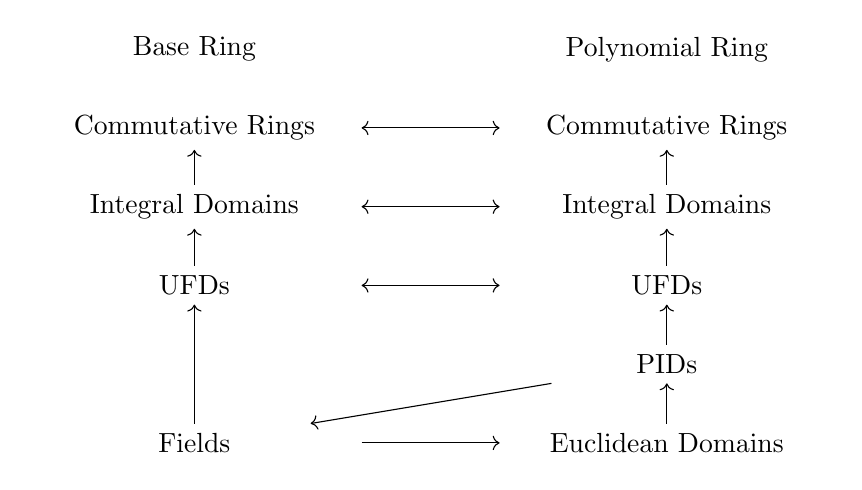
\begin{tikzpicture}[
      node distance=2cm,
      box/.style={
          text width=4cm,
          align=center
      }
      ]
      % Nodes for ring types
      \node[box] (base) at (-3,0) {Base Ring};
      \node[box] (poly) at (3,0) {Polynomial Ring};

      \node[box] (comm) at (-3,-1) {Commutative Rings};
      \node[box] (p_comm) at (3,-1) {Commutative Rings};
      \node[box] (int) at (-3,-2) {Integral Domains};
      \node[box] (p_int) at (3,-2) {Integral Domains};
      \node[box] (ufd) at (-3,-3) {UFDs}; % Added UFD between ID and PID
      \node[box] (p_ufd) at (3,-3) {UFDs}; % Added UFD between ID and PID
      \node[box] (field) at (-3,-5) {Fields}; % Moved Fields down
      \node[box] (p_pid) at (3,-4) {PIDs}; % Moved PID down
      \node[box] (p_euc) at (3,-5) {Euclidean Domains}; % Moved ED down
      
      % Left path arrows
      \draw[<-] (comm) -- (int);
      \draw[<-] (int) -- (ufd);
      \draw[<-] (ufd) -- (field);

      \draw[<-] (p_comm) -- (p_int);
      \draw[<-] (p_int) -- (p_ufd);
      \draw[<-] (p_ufd) -- (p_pid);
      \draw[<-] (p_pid) -- (p_euc);

      \draw[<->] (comm) -- (p_comm);
      \draw[<->] (int) -- (p_int);
      \draw[<->] (ufd) -- (p_ufd);
      \draw[->] (p_pid) -- (field);
      \draw[->] (field) -- (p_euc);
    \end{tikzpicture}
    \caption{Basic hierarchy of rings with UFDs included.} 
    \label{fig:poly_hierarchy}
  \end{figure}

\subsection{Commutative Polynomial Rings}

  We begin our study by looking at commutative polynomial rings. The first order of business is to be able to tell when such $R[x]$ is commutative. There is a simple condition for this. 

  \begin{theorem}[Conditions for $R\lbrack x \rbrack$ to be Commutative]
    Let $R$ be a ring and $S = \{x_1, \ldots, x_m\}$ be a finite set of indeterminates. $R$ is a commutative ring iff $R[x]$ is a commutative ring. 
  \end{theorem}
  \begin{proof}
    We prove bidirectionally. 
    \begin{enumerate}
      \item $(\rightarrow)$ If $R$ is commutative then given $a, b \in R$, we have $(ax^i) (b x^j) = a (x^i b) x^j = (ab)(x^i x^j) = (ba) (x^j x^i) = (b x^j) (a x^i)$, and so from distributive property $R[x]$ is commutative. 
      \item $(\leftarrow)$ This is trivial since given $R[x]$ commutative, take $a, b \in R \subset R[x]$, and so $ab = ba$ in $R[x]$ implies commutativity in $R$. 
    \end{enumerate}
  \end{proof}

  Now we associate long division with Euclidean domains, and this is the case in the integers. However, for polynomials, we can state a slightly weaker form in that we can divide any polynomial by not just any other polynomial, but a \textit{monic} polynomial. 

  \begin{theorem}[Division Algorithm Exists for Monic Divisors]
    \label{thm:poly-long-division}
    Given any ring $R$, with $f(x), d(x) \in R[x]$ where the leading coefficient of $d(x)$ is a unit, a division algorithm exists. That is, we can find a $q(x), r(x) \in R$ where 
    \begin{equation}
      f(x) = q(x) d(x) + r(x), \qquad 0 \leq \deg{r(x)} < \deg{d(x)}
    \end{equation}
  \end{theorem}
  \begin{proof}
    We construct how to do so. This is because at each step, you only need to divide the leading coefficient of the divisor into the leading coefficient of the polynomial you have left. 
  \end{proof}

  \begin{example}[Polynomial Long Division] 
    We apply the steps in the proof above to the example. 
    \begin{center}
      \polylongdiv{x^3 + 4x^2 - x + 7}{x - 2}
    \end{center}
  \end{example} 

  Now let's introduce polynomial roots and how they relate to the factors and evaluation of a function $f(x)$. 

  \begin{corollary}[Root-Factor Theorem]
    Given a commutative ring $R$ and $f(x) \in R[x]$, $(x - c)$ is a factor of $f(x)$, i.e. can be factored into 
    \begin{equation}
      f(x) = (x - c) q(x) 
    \end{equation}
    for some $q(x) \in R[x]$ of degree $\deg(f) - 1$ if and only if $f(c) = 0$.\footnote{Note that this is not true for an arbitrary ring. $R$ must be commutative at least.}
  \end{corollary} 
  \begin{proof}
    We prove for when $R$ is a field $F$, but it turns out that the theorem also holds for commutative rings $R$. 
    \begin{enumerate}
      \item $(\rightarrow)$. Given that $(x - c)$ is a factor of $f(x)$, this means that by the Euclidean algorithm $f(x) = (x - c) q(x)$ for some $q(x)$, and so $f(c) = (c - c) q(c) = 0$. 
      \item $(\leftarrow)$. Given that $f(c) = 0$. By the remainder theorem this means that when we divide $f(x)$ by $(x - c)$, the remainder is $f(c) = 0$, and so $f(x) = (x - c) q(x) + 0 = (x - c) q(x) \implies (x - c)$ is a factor of $f(x)$. 
    \end{enumerate}
  \end{proof}

  \begin{corollary}[Remainder Theorem]
    Let $c \in F$ and $f(x) \in F[x]$. When we divide $f(x)$ by $g(x) = x - c$, the remainder is $f(c)$. 
  \end{corollary}
  \begin{proof}
    By the division algorithm, 
    \begin{equation}
      f(x) = (x - c) q(x) + r(x) \implies f(c) = (c - c) q(c) + r(c) = r(c)
    \end{equation}
  \end{proof} 

  \begin{definition}[Multiplicity]
    A root $c$ of polynomial $f(x) \in F[x]$ is called simple if $f(x)$ is not divisible by $(x - c)^2$ and multiple otherwise. The \textbf{multiplicity} of a root $c$ is the maximum k such that $(x - c)^k$ divides $f(x)$ .
  \end{definition} 

  Often, we refer to a polynomial having no repeated roots as being \textit{square-free}. 

  Finally, let's talk about what quotient polynomial rings look like. 

  \begin{example}[Counting Ring Homomorphisms]
    We wish to count the number of ring homomorphisms 
    \begin{equation}
      \phi: \frac{\mathbb{Z}}{\langle x^3 + y^2 - 1 \rangle} \to \mathbb{Z}_7
    \end{equation}
    Note that any such homomorphism $\phi$ induces by composition a unique canonical homomorphism $f: \mathbb{Z}[x, y] \to \mathbb{Z}_7$. $f$ must map $1$ to $1$, so it leaves a total of 49 choices for what it can map $x, y$ to. Now since the kernel must contain the ideal $\langle x^3 + y^2 - 1 \rangle$, this means that we would like 
    \begin{equation}
      f(x^3 + y^2 - 1) = f(x)^3 + f(y)^2 - 1 = 0
    \end{equation}
    and from this we can count. 
  \end{example}

\subsection{Polynomial Integral Domains}

  Now we talk about when $R[x]$ becomes an integral domain. When is this the case? 

  \begin{theorem}[Conditions for $R\lbrack x \rbrack$ to be Integral Domain]
    Let $R$ be a ring and $S = \{x_1, \ldots, x_m\}$ be a finite set of indeterminates. $R$ is an integral domain iff $R[x]$ is an integral domain. 
  \end{theorem}
  \begin{proof}
    It suffices to prove the domain property since commutativity is already proved. 
    \begin{enumerate}
      \item $(\rightarrow)$. Assume $R$ is a domain. Now take any two nonzero polynomials $f(x), g(x) \in R[x]$. Then look at their leading term $ax^n$ and $bx^n$. The leading coefficient of $(fg)(x)$ is $(ab) x^{n+m}$, and since $R$ is a domain $ab \neq = 0 \implies (fg)(x) \neq 0$. So $R[x]$ is a domain. 
      \item $(\leftarrow)$. This is trivial since given $R[x]$ integral domain, take $a, b \in R \subset R[x]$ with $a, b \neq 0$, and so $ab \neq 0$ since $R[x]$ is a domain. Therefore $R$ is a domain. 
    \end{enumerate}
  \end{proof}

  We can see how $R[x]$ fails to be a domain when $R$ is not an integral domain. 

  \begin{example}[Product of Two Linear Polynomials is $0$]
    Given $f, g \in \mathbb{Z}_6 [x]$ with $f(x) = 2x + 4$ and $g(x) = 3x + 3$, we have 
    \begin{equation}
      f(x) \cdot g(x) = (2x + 4)(3x + 3) = 6x^2 + 18 x + 12 = 0
    \end{equation}
  \end{example}

  In addition to the results we derived for general integral domains, what special results can we derive for that of polynomial rings? First, we have the familiar property of the degree of a product of two polynomials. 

  \begin{lemma}[Degree of Product of Polynomials]
    Given integral domain $R[x]$ and $f(x), g(x) \in R[x]$, we have 
    \begin{equation}
      \deg{fg(x)} = \deg{f(x)} + \deg{g(x)}
    \end{equation}
  \end{lemma}
  \begin{proof}
    Trivial. Consider the leading coefficient of $f(x), g(x)$. 
  \end{proof}

  Now the integral domain property gives us also a nice bound on the number of roots. If $R[x]$ was not an integral domain, then $R$ is not an integral domain, and so there exists zero divisors $a, b \in R$ s.t. $ab = 0$. Now consider 
  \begin{equation}
    f(x) = (x - a) (x - b) = x^2 - (a + b) x + ab = x^2 - (a + b) x
  \end{equation}
  and we have found a degree two polynomial having at least three roots. We can also state the converse of this. 

  \begin{theorem}[Bounds on Number of Roots]
    Let $R[x]$ be an integral domain and $f(x) \in R[x]$. Then $f(x)$ has at most $\deg{f(x)}$ roots. 
  \end{theorem}
  \begin{proof}
    Let us consider the equation $f(x) = x^2 - m = 0$, where $m \in R$ is nonzero. Suppose $f(x)$ has more than $2$ roots, i.e. 
    \begin{equation}
      x^2 - m = (x - a)(x - b) = (x - c) (x - d), \qquad a, b, c, d \in R
    \end{equation}
    Let $c \neq a, b$. Then $(c - a)(c - b) = 0 (c - d) = 0$, which implies that $R$ is not an integral domain. 
  \end{proof}

  Therefore, the number of roots of a polynomial---counted with multiplicity---does not exceed the degree of this polynomial. Furthermore, these numbers are equal if and only if the polynomial is a product of linear factors, which has its own terminology. That is, given a polynomial $f(x)$, we can view it as an element of multiple polynomial rings $R[x]$. The properties of the ring $R$ will determine the properties of $f(x)$ as an element of $R[x]$. 

  \begin{theorem}[Splitting Ring/Field]
    A polynomial $f(x)$ is said to \textbf{split} in $R[x]$ if $f(x)$ can be factored into only linear factors. 
  \end{theorem}

\subsection{Polynomial Unique Factorization Domains}

  What's great about UFDs $R$ is that we can relate the decomposition of polynomials in $R[x]$ to the decomposition in $F[x]$, where $F$ is the field of fractions of $R$.\footnote{It is a field since $R$ is an integral domain.} This is precisely stated through Gauss's lemma. 

  \begin{lemma}[Gauss's Lemma]
    Let $R$ be a UFD and $F$ be its field of fractions. Then reducibility in $F[x]$ implies reducibility in $R[x]$. That is, given $f(x) \in R[x]$, if there exists $g(x), h(x) \in F[x]$ s.t. $g(x) h(x) = f(x)$, then there exists $\bar{g}(x), \bar{h}(x) \in R[x]$ s.t. $\bar{g}(x) \bar{h}(x) = f(x)$. 
  \end{lemma}
  \begin{proof}
    We prove for $R = \mathbb{Z}$. We can find $k, l \in \mathbb{Z}$ s.t. $g_1 (x) = k g(x)$ and $h_1 (x) = l h(x)$ have integer coefficients, i.e. $g_1, h_1 \in \mathbb{Z}[x]$. Then, $k l f(x) = g_1 (x) h_1 (x) \in \mathbb{Z}[x]$. Let $p$ be a prime factor of $kl$. We have 
    \begin{equation}
      0 \equiv \bar{k} \bar{l} \bar{f} (x) \equiv \bar{g}_1 (x) \bar{h}_1 (x) \text{ in } \mathbb{Z}_p [x]
    \end{equation}
    Since $\mathbb{Z}_p$ is an integral domain, $\mathbb{Z}_p [x]$ is an integral domain, and so $\bar{g}_1$ or $\bar{h}_1$ must be $0$. WLOG let it be $\bar{g}_1$. Then every coefficient of $g_1 (x)$ is divisible by $p$, and we can write it in the form $g_2(x) = p g_1 (x)$. Therefore, 
    \begin{equation}
      p(x) \cdot \frac{kl}{p} = \underbrace{\frac{g_1 (x)}{p}}_{g_2 (x)} \cdot \underbrace{h_1 (x)}_{h_2 (x)} \iff f(x) \frac{kl}{p} = g_2 (x) h_2 (x)
    \end{equation}
    Since there are only finitely many prime divisors, we do this for all prime factors of $kl$, and we have 
    \begin{equation}
      f(x) = g_n (x) h_n (x), \qquad g_n, h_n \in \mathbb{Z}[x]
    \end{equation}
  \end{proof}

  Therefore in the specific case of $\mathbb{Z}$, Gauss's lemma says that decompositions in $\mathbb{Q}[x]$ imply decompositions in $\mathbb{Z}[x]$! By looking at the contrapositive, to check irreducibility in $\mathbb{Q}[x]$, it suffices to check irreducibility in $\mathbb{Z}[x]$. 

  \begin{theorem}[Conditions for $R\lbrack x \rbrack$ to be a UFD]
    Let $R$ be a ring and $S = \{x_1, \ldots, x_m\}$ be a finite set of indeterminates. $R$ is a UFD implies $R[S]$ is a UFD. 
  \end{theorem}
  \begin{proof}
    By induction, it suffices to show for when $S = \{x\}$. Let $F$ be the field of fractions of $R$. Since $F$ is a field, $F[x]$ is Euclidean domain and hence a PID. So every polynomial in $R[x]$ has a unique factorization in $F[x]$. By Gauss's lemma, this factorization is actually in $R[x]$. 
  \end{proof}

  Note that this is \textit{not} true in arbitrary rings, i.e. non-UFDs. 

  \begin{example}[Linear Polynomial with 3 Roots]
    Consider $f(x) = x^2 - 1 \in \mathbb{Z}_8 [x]$, a commutative ring. Then $1, 3, 5, 7$ are all roots of $f(x)$, which is greater than its degree. Furthermore, it has two different factorizations 
    \begin{equation}
      x^2 - 1 = (x + 1)(x - 1) = (x + 3)(x - 3)
    \end{equation}
  \end{example} 

  Another milestone theorem is that in UFDs, we can use the rational root theorem to reduce our search space of roots in the field of fractions.  

  \begin{theorem}[Rational Root Theorem for UFDs]
    Let $R$ be a UFD and 
    \begin{equation}
      f(x) = a_n x^n + \ldots + a_1 x + a_0 \in R[x] 
    \end{equation}
    If $K$ is the fraction field of $R$ and $f(k) = 0$ with $k = \frac{p}{q}$ for $p, q$ coprime, then $p \mid a_0$ and $p \mid a_n$. 
  \end{theorem}
  \begin{proof}
    Given that $r/s$ is a root, we have 
    \begin{equation}
      a_n (r/s)^n + \ldots + a_0 = 0
    \end{equation}
    Multiplying by $s^n$, we get 
    \begin{equation}
      a_n r^n + a_{n-1} r^{n-1} s + \ldots + a_1 s^{n-1} r + a_0 s^n = 0
    \end{equation}
    and putting this equation on mod $r$ and mod $s$ implies that $r | a_0 s^n$ and $s | a_n r^n$, respectively. But since we assumed that $\gcd (r, s) = 1$, $r | a_0$ and $s | a_n$. 
  \end{proof}

  \begin{corollary}[Rational Root Theorem for Integers]
    Let $a_n x^n + \ldots + a_0 \in \mathbb{Z}[x]$. If $r/s \in \mathbb{Q}$ with $\gcd(r, s) = 1$, then $r \mid a_0$ and $s \mid a_n$. 
  \end{corollary}

  \begin{example}[Reducibility of Integer Polynomials]
    Let $f(x) = x^4 - x^3 + 2$. The rational roots are in the set $S = \{\pm 1, \pm2 \}$, but none of them work since $f(\pm1), f(\pm2) \neq 0$. By degree considerations and Gauss's lemma, if $f(x)$ is reducible, then 
    \begin{equation}
      f(x) = (x^2 + ax + b) (x^2 + cx + d), \qquad a, b, c, d \in \mathbb{Z}
    \end{equation}
    We know that $bd \in S$, with $a + c = -1$, $d + b + ac = 0$, and so on for each coefficients. We can brute force this finite set of possibilities. 
  \end{example}

  \begin{example}
    We claim that $x^4 - 22x^2 + 1 = (x - (\sqrt{6} + \sqrt{5})) (x - (\sqrt{6} - \sqrt{5})) (x - (-\sqrt{6} + \sqrt{5})) (x - (-\sqrt{6} - \sqrt{5})) $ is irreducible in $\mathbb{Q} [x]$. By the rational root theorem $\pm 1$ are the possible rational roots, but plugging it into reveals that they aren't roots. Now if $x^4 - 22x^2 + 1$ factors it must factor as a product of monic quadratic polynomials in $\mathbb{Z}[x]$ by Gauss's Lemma. Therefore, 
    \begin{equation}
      (x^2 + ax + b) (x^2 + cx + d) = x^4 - 22x^2 + 1
    \end{equation}
    Then $a + c = 0, bd = 1, ad + bc = 0, d + b + ac = 22$. We can derive this and find that there are no solutions, and so it is irreducible. 
  \end{example}

  A great way to check irreducibility is to check in mod $p$. 

  \begin{theorem}
    Let $f(x) = a_n x^n + \ldots + a_0 \in \mathbb{Z}[x]$. If $p \nmid a_n$ and $f \in \mathbb{Z}_p [x]$ is irreducible, then $f$ is irreducible in $\mathbb{Q}[x]$.\footnote{May need to verify this again.}
  \end{theorem}
  \begin{proof}
    Suppose that $f(x) = g(x) h(x) \in \mathbb{Z}[x]$ with $\deg(g), \deg(h) > 0$. Then 
    \begin{equation}
      f(x) \equiv g(x) h(x) \text{ in } \mathbb{Z}_p [x]
    \end{equation}
    Since $f(x)$ is irreducible in $\mathbb{Z}_p [x]$, we must have that one of $g(x)$ or $h(x)$ has degree $0$ in $\mathbb{Z}_p [x]$. WLOG let it be $g(x)$, but this means that the leading coefficient of $g(x)$ must be divisible by $p \implies$ leading coefficient of $f(x)$ is divisible by $p \iff p \mid a_n$. 
  \end{proof}

  \begin{example}
    $x^4 + x + 1$ is irreducible in $\mathbb{Z}_2 [x]$. So we can extend this to $\mathbb{Z}[x]$ to see that \textit{all} fourth degree polynomials of form $a x^4 + b x^3 + c x^2 + dx + e$, which $a, d, e$ odd and $b, c$ even is irreducible in $\mathbb{Q}[x]$. 
  \end{example}

  This is a powerful theorem to quickly find a large class of polynomials that are irreducible. However, being reducible in $\mathbb{Z}_p [x]$ does not imply reducibility in $\mathbb{Q}$. In fact, there are polynomials $f(x) \in \mathbb{Z}[x]$ which are irreducible but reducible in $\mathbb{Z}_p$ for \textit{every} prime $p$. 

  \begin{theorem}[Eisenstein's Criterion]
    Let $f(x) = a_n x^n + \ldots + a_0 \in \mathbb{Z}[x]$ and $p \in \mathbb{Z}$ a prime s.t. $p \nmid a_n$, $p \mid a_i$ for $i = 0, \ldots, a_{n-1}$, and $p^2 \nmid a_0$. Then $f(x)$ is irreducible in $\mathbb{Q}[x]$. 
  \end{theorem}
  \begin{proof}
    Suppose that $f(x) = g(x) h(x) \in \mathbb{Q}[x]$ with $\deg(g), \deg(h) > 0$. Then, by Gauss's lemma, $g, h \in \mathbb{Z}[x]$. Reducing the equations mod $p$, 
    \begin{equation}
      f(x) = g(x) h(x) \text{ in } \mathbb{Z}_p [x]
    \end{equation}
    But $f(x) = a_n x^n$. By unique factorization theorem in $\mathbb{Z}_p [x]$, $g, h \in \mathbb{Z}_p [x]$ must be products of units and prime factors of $a_n x^n$, which are $\{x\}$. Therefore, let 
    \begin{equation}
      g(x) = b_m x^m, h(x) = \frac{a_n}{b_m} x^{n-m} \in \mathbb{Z}_p [x]
    \end{equation}
    with $\deg(g) = m > 0$ and $\deg(h) = n - m > 0$ in $\mathbb{Z}[x]$. This implies that the constant coefficients of $g(x), h(x)$ are divisible by $p$, which implies that the constant coefficients of $f(x) = g(x) h(x)$ are divisible by $p^2$, a contradiction. 
  \end{proof}

  \begin{example}[Easy Checks for Irreducibility with Eisenstein]
    Listed. 
    \begin{enumerate}
      \item $x^{13} + 2x^{10} + 4x + 6$ is irreducible in $\mathbb{Q}[x]$ by Eisenstein for $p = 2$. 
      \item $x^3 + 9x^2 + 12x + 3$ is irreducible in $\mathbb{Q}[x]$ by Eisenstein for $p = 3$. 
      \item Let $f(x) = x^4 + x^3 + x^2 + x + 1$. Then, we know that $f(x) = \frac{x^5 - 1}{x-1}$ and so 
      \begin{align}
        f(x + 1) & = \frac{(x + 1)^5 - 1}{(x + 1) - 1} \\
                 & = \frac{1}{x} \bigg( x^5 + \binom{5}{1} x^4 + \binom{5}{2} x^3 + \binom{5}{3} x^2 + \binom{5}{4} x + \binom{5}{5} - 1 \bigg) \\
                 & = x^4 + 5x^3 + 10 x^2 + 10x + 5
      \end{align}
      So all nonleading coefficients are divisible by $5$ exactly once, which by Eisenstein implies that $f(x+1)$ is irreducible which implies that $f(x)$ is irreducible. 
    \end{enumerate}
  \end{example}

  Since UFDs have unique GCDs, we can state the following. 

  \begin{theorem}[GCD of Two Polynomials in a UFD Exist]
    Given nonzero polynomials $f(x), g(x) \in F[x]$, let 
    \begin{equation}
      S = \{h(x) \in F[x] \mid h(x) = a(x) f(x) + b(x) g(x) \text{ for some } a(x), b(x) \in F[x] \}
    \end{equation} 
    Then there exists some polynomial $d(x) \in S$ of smallest degree, and every $h(x) \in S$ is divisible by $d(x)$. 
  \end{theorem}
  \begin{proof}
    The existence is trivial since by the well-ordering principle on the degrees of polynomials in $S$, such a minimal degree must exist. Now we prove the second claim by proving $d(x) \mid f(x)$. We apply the division algorithm to write 
    \begin{equation}
      f(x) = q(x) d(x) + r(x)
    \end{equation}
    If $r(x) = 0$, then by root factor theorem we are done. If $r(x) \neq 0$, we then write 
    \begin{align}
      r(x) & = f(x) - q(x) d(x) \\ 
           & = f(x) - \big( s(x) f(x) + t(x) g(x) \big) q(x) \\ 
           & = \big( 1 - s(x) q(x) \big) f(x) - \big( t(x) q(x) \big) g(x) \in S
    \end{align}
    Since $r(x) \in S$ due to its form, the fact that $\deg(r(x)) < \deg(d(x))$ contradicts the way that $d(x)$ was chosen. Therefore $r(x) = 0$. It turns out that $d(x)$ is unique up to a constant factor. 
  \end{proof}

  The algorithmic way for computing the GCD is done the same way by performing Euclidean algorithm on two polynomials: dividing on by the other, taking the remainder, and dividing the lesser degree by the remainder again, until the remainder is $0$. 

\subsection{Polynomial Euclidean Domains}

  \begin{definition}[Polynomial Euclidean Domains]
    We call $F[x]$ a \textbf{Euclidean domain} if for all $f(x), g(x) \in F[x]$ and $g(x) \neq 0$, there exists polynomials $q(x), r(x)$ such that 
    \begin{equation}
      f(x) = q(x) g(x) + r(x), \qquad 0 \leq \deg(r) < \deg(g)
    \end{equation}
    where $\deg$ is the norm.
  \end{definition}

  \begin{example}[]
    
  \end{example}

  We again start with the conditions for a polynomial ring to be a Euclidean domain. It is \textit{not} the case that $R$ should be a Euclidean domain. In fact, we need something stronger. 

  \begin{theorem}[Conditions for $R\lbrack x \rbrack$ to be Euclidean Domain]
    Let $R$ be a ring and $S = \{x_1, \ldots, x_m\}$ be a finite set of indeterminates. $F$ is a field implies $R[x]$ is a Euclidean domain, with norm $N(f(x)) = \deg{f(x)}$. That is, given polynomials $f(x), g(x) \in F[x]$, there are unique polyomials $q(x), r(x) \in F[x]$ s.t. 
    \begin{equation}
      f(x) = q(x) g(x) + r(x), \qquad \deg(r(x)) < \deg(g(x))
    \end{equation} 
  \end{theorem}
  \begin{proof}
    We first prove existence. If $\deg(f(x)) < \deg(g(x))$, then we can trivially set $q(x) = 0, r(x) = f(x)$. Therefore we can assume that $\deg(f(x)) \geq \deg(g(x))$. We can prove this by strong induction on $k = \deg(f(x))$. Assume that $\deg(f(x)) = 1$. Then if $\deg(g(x)) > 1$ it is trivial as before, so we show for $\deg(g(x)) = 1$. So let 
    \begin{equation}
      f(x) = a_1 x + a_0, \qquad g(x) = b_1 x + b_0 
    \end{equation}
    and we can find the solutions 
    \begin{equation}
      f(x) = \frac{a_1}{b_1} g(x) + \bigg( a_0 - \frac{a_1 b_0}{b_1} \bigg)
    \end{equation} 
    Now suppose that the results is known for whenver $\deg(f(x)) \leq k$ and we have a polynomial $F(x) = a_{k+1} x^{k+1} + \ldots a_0$ of degree $k+1$. Then we must check that there exists a quotient and remainder for $0 \leq \deg(g(x)) = m \leq k + 1$. Note that the coefficients of $x^{k+1}$ in $F(x)$ and in the polynomial $\frac{a_{k+1}}{b_m} x^{k+1-m} g(x)$ are the same, so the polynomial 
    \begin{equation}
      f(x) = F(x) - \frac{a_{k+1}}{b_m} x^{k+1-m} g(x) 
    \end{equation}
    has degree at most $k$. Thus by our induction hypothesis we can write $f(x) = q(x) g(x) + r(x)$, and so 
    \begin{align}
      F(x) & = f(x) + \frac{a_{k+1}}{b_m} x^{k+1-m} g(x) \\
           & = q(x) g(x) + r(x) + \frac{a_{k+1}}{b_m} x^{k+1-m} g(x) \\ 
           & = \bigg( q(x) + \frac{a_{k+1}}{b_m} x^{k+1-m} \bigg) g(x) + r(x)
    \end{align} 
    which is indeed a decomposition. Now to prove uniqueness, suppose we had two different decompositions 
    \begin{equation}
      f(x) = q(x) g(x) + r(x) = q^\prime (x) g(x) + r^\prime (x) \implies \big( q(x) - q^\prime (x) \big) g(x) = r(x) - r^\prime (x)  
    \end{equation}  
    IF $q(x) \neq q^\prime (x)$, then the degree of the LHS is at least $\deg(g(x))$, while the degree of the RHS must be strictly less, a contradiction. 
  \end{proof}

  Note that alternatively, we have shown from \ref{thm:poly-long-division} that the leading coefficient of the divisor $g(x)$ must be a unit in $R$. For a field, every element is a unit, and we are done. 

  \begin{theorem}[PID Polynomial Rings Implies Underlying is a Field]
    \label{thm:pid-field}
    $R[x]$ is a PID implies $R$ is a field.
  \end{theorem}
  \begin{proof}
    Assume that $R[x]$ is a PID. Since $R$ is a subring of $R[x]$, then $R$ must be an integral domain. The ideal $\langle x \rangle$ is a nonzero prime ideal in $R[x]$ because $R[x]/\langle x \rangle$ is isomorphic to the integral domain $R$. Since every nonzero prime ideal in a PID is a maximal ideal, $\langle x \rangle$ is a maximal ideal, hence the quotient $R$ is a field. 
  \end{proof} 

  From this theorem, we can see that if a polynomial ring is a PID, then we know that it is automatically a Euclidean domain, so it suffices to only consider the case of Euclidean domains, which is why we skip PID polynomial rings. 

  Now we talk about the behavior of polynomials as functions. Sometimes, we may have two different polynomials but they may define the same function from $R$ to $R$! 

  \begin{example}[Polynomials as Same Function]
    Given $f, g \in \mathbb{Z}_2 [x]$, 
    \begin{equation}
      f(x) = x \sim g(x) = x^2
    \end{equation} 
  \end{example} 

  With an additional condition on a field, we can guarantee that each polynomial determines a different function. 

  \begin{theorem}[Uniqueness of Polynomials over Field]
    If the field $\mathbb{F}$ is infinite, then different polynomials in $\mathbb{F}[x]$ determine different functions. 
  \end{theorem}

  \begin{theorem}[Interpolation]
    For any collection of given field values $y_1, y_2, ..., y_n \in F$ at given distinct points $x_1, x_2, ..., x_n \in F$, there exists a unique polynomial $f \in F[x]$ with deg$\, f < n$ such that
    \begin{equation}
      f(x_i) = y_i, \quad i = 1, 2, ..., n
    \end{equation}
    This is commonly known as the \textbf{interpolation problem}, and when $n = 2$, this is called \textbf{linear interpolation}. 
  \end{theorem} 

\subsection{Algebraically Closed Fields} 

  Now that we have seen some examples of fields, what properties would we like it to have? Going back to polynomials, recall that if $F$ is a field, then $F[x]$ as a Euclidean domain gave us a lot of nice properties, such as admitting a unique factorization of irreducible polynomials. However, we have only proved that the number of roots is \textit{at most} the degree $n$, but not that it actually reaches $n$. In fact, in a more extreme case, a polynomial may not even factor \textit{at all} in $F[x]$, since it could be irreducible. So while we have defined an upper bound for the number of roots for a polynomial, we have not determined whether a polynomial has any roots at all, i.e. a lower bound. 

  We don't have much \textit{control} over what these irreducible polynomials can look like. We may have to check---either through theorems or manually---that a polynomial or arbitrary degree is irreducible. If we would like to assert that all irreducible polynomials must be of smallest degree---that is, linear---then such a field is called \textit{algebraically closed}. 
  This algebraic closed property asserts also that the lower bound on the number of (non-unique) factors is $n$. 

  \begin{definition}[Algebraically Closed Field]
    A field $F$ is \textbf{algebraically closed} if every polynomial of positive degree (i.e. non-constant) in $F[x]$ has at least one root in $F$. 
  \end{definition}

  This is equivalent to saying that every polynomial can be expressed as a product of first degree polynomials. To extend our analysis more, we can talk about the multiplicity of these factors, which just tells us more about how many unique and non-unique factors a polynomial has. 

  \begin{example}[Reals are not Algebraically Closed]
    $\mathbb{R}$ is not algebraically closed since we can identify the polynomial $f(x) = x^2 + 1 \in \mathbb{R}[x]$ which does not have any roots in $\mathbb{R}$. Consequently, any subfield of $\mathbb{R}$ (which contains $1$) such as $\mathbb{Q}, \mathbb{Q}(\sqrt{2}), \ldots$ are not algebraically closed. 
  \end{example}

  It turns out that the complex numbers are algebraically closed, which is presented with the following grand name. Ironically, this theorem cannot be proven with algebra alone. We need complex analysis.\footnote{Gauss proved this for the first time in 1799.} 

  \begin{theorem}[Fundamental Theorem of Algebra]
    Suppose $f \in \mathbb{C}[x]$ is a polynomial of degree $n \geq 1$. Then $f(x)$ has a root in $\mathbb{C}$. It immediately follows from induction that it can be factored as a product of linear polynomials in $\mathbb{C}[x]$. 
  \end{theorem}
  \begin{proof}
    WLOG we can assume that $f$ is monic: $f(z) = z^n + a_{n-1} z^{n-1} + \ldots + a_1 z + a_0$. Since $\mathbb{C}$ is a field, we can set 
    \begin{equation}
      f(z) = z^n \bigg( 1 + \frac{a_{n-1}}{z} + \frac{a_{n-2}}{z^2} + \ldots + \frac{a_0}{z_n} \bigg)
    \end{equation} 
    Since 
    \begin{equation}
      \lim_{|z| \rightarrow \infty} \bigg( 1 + \frac{a_{n-1}}{z} + \frac{a_{n-2}}{z^2} + \ldots + \frac{a_0}{z_n} \bigg) = 0
    \end{equation}
    there exists a $R > 0$ s.t. 
    \begin{equation}
      |z| > R \implies \bigg| 1 + \frac{a_{n-1}}{z} + \frac{a_{n-2}}{z^2} + \ldots + \frac{a_0}{z_n} \bigg| < \frac{1}{2}
    \end{equation}
    and hence 
    \begin{equation}
      |z| > R \implies |f(z)| > |z|^n \cdot \bigg( 1 - \frac{1}{2} \bigg) > \frac{R^n}{2}
    \end{equation}
    So $z$ cannot be a root if $|z| > R$. On the other hand, $f(z)$ is continuous (under the Euclidean topology) and so on the compact set $\{z \in \mathbb{C} \mid |z| \leq R\}$, $|f(z)|$ achieves a minimum value say at the point $z_0$. We claim that $\min_z f(z) = 0$. 

    For convenience, we let $z_0 = 0$ (we can do a change of basis on the polynomial) and assume that the minimum is some positive number, i.e. $f(0) = a_0 \neq 0$. Let $j$ be the smallest positive integer such that $a_j = 0$. Let 
    \begin{equation}
      g(z) = \frac{a_{j+1}}{a_j} z + \ldots + \frac{a_n}{a_j} z^{n-j} \implies f(z) = a_0 + a_j z^j \big( 1 + g(z) \big) 
    \end{equation}
    We set $\gamma = \sqrt[j]{-a_0/a_j}$ and consider the values of 
    \begin{align}
      f(t \gamma) & = a_0 + a_j (t\gamma)^j \big( 1 + g(t\gamma) \big) \\
                  & = a_0 - a_0 t^j \big(1 + g(t \gamma) \big) \\
                  & = a_0 \big\{ 1 - t^j \big(1 + g(t \gamma) \big) \big\}
    \end{align} 
    for $t > 0$. For $t$ sufficiently small, we have 
    \begin{equation}
      |g(t \gamma)| = \bigg| \frac{a_{j+1}}{a_j} (t \gamma) + \ldots + \frac{a_n}{a_j} (t \gamma)^{n-j} \bigg| < \frac{1}{2} 
    \end{equation}
    and for such $t$, this implies 
    \begin{equation}
      |f(t \gamma)| = |a_0| |1 - t^j (1 + g(t \gamma))| \leq |a_0| |1 - t^j/2| < |a_0|
    \end{equation}
    and so $z_0$ cannot have been the minimum of $|f(z)|$. Therefore, the minimum value must be $0$.  
  \end{proof}

  Great, so through this theorem, we can work in any subfield of $\mathbb{C}$ and guarantee that will have all of its roots in $\mathbb{C}$. 

  \begin{corollary}[$\mathbb{C}$ is algebraically closed]
    $\mathbb{C}$ is algebraically closed, i.e. $\mathbb{C}$ is a splitting field of $\mathbb{C}[x]$. 
  \end{corollary}

  Put more succinctly, the impossibility of defining division on the ring of integers motivates its extension into the field of rational numbers. Similarly, the inability to take square roots of negative real numbers forces us to extend the field of real numbers to the bigger field of complex numbers. 

  \begin{theorem}[Complex Roots Come in Conjugate Pairs]
    If $\alpha$ is a complex root of polynomial $f \in \mathbb{R}[x]$, then $\bar{\alpha}$ is also a root of the polynomial. Moreover, $\bar{\alpha}$ has the same multiplicity as $\alpha$. 
  \end{theorem}
  \begin{proof}
    Note that conjugation is an automorphism (in fact an $\mathbb{R}$-automorphism over $\mathbb{C}$). Therefore, if $\alpha \in \mathbb{C}$ is a root, then 
    \begin{align}
      f(\bar{\alpha}) & = a_n f(\bar{\alpha})^n + \ldots a_1 f(\bar{\alpha}) + a_0 \\ 
                      & = a_n \overline{f(\alpha)}^n + \ldots a_1 \overline{f(\alpha)} + a_0 \\  
                      & = \bar{0} = 0
    \end{align}
  \end{proof}

  This theorem has a lot of consequences on the reducibility of polynomials in the reals. 

  \begin{corollary}[Odd Degree Polynomials have At Least 1 Real Root]
    Every polynomial $f \in \mathbb{R}[x]$ of odd degree has at least one real root. 
  \end{corollary}
  \begin{proof}
    Assume that $n = \deg{f}$ was odd and there were $m$ roots, with $m$ even. Then there are $n - m$ roots, which is an odd number of complex roots, which contradicts the previous theorem. 
  \end{proof}
  \begin{proof}
    Just for fun, a proof using analysis is as such. Without loss of generality we can assume that the leading coefficient of $f$ is positive. Then
    \begin{equation}
      \lim_{x \rightarrow + \infty} f(x) = + \infty, \; \lim_{x \rightarrow -\infty} f(x) = -\infty
    \end{equation}
    By the intermediate value theorem, there must be some point where $f$ equals $0$. 
  \end{proof}

  \begin{corollary}[Real Polynomials Factors Into Linear and Quadratic Terms]
    Every nonzero polynomial in $\mathbb{R}[x]$ factors into a product of linear terms and quadratic terms with negative discriminants. 
  \end{corollary}

  \begin{example}
    \begin{align*}
      x^5 - 1 & = (x-1) \bigg( x - \Big( \cos{\frac{2\pi}{5}} + i \sin{\frac{2\pi}{5}}\Big) \bigg) \bigg( x - \Big( \cos{\frac{2\pi}{5}} - i \sin{\frac{2\pi}{5}}\Big) \bigg) \\
      & \times \bigg( x - \Big( \cos{\frac{4\pi}{5}} + i \sin{\frac{4\pi}{5}}\Big) \bigg) \bigg( x - \Big( \cos{\frac{4\pi}{5}} - i \sin{\frac{4\pi}{5}}\Big) \bigg) \\
      & = (x-1) \bigg( x^2 - \frac{\sqrt{5} - 1}{2} x + 1\bigg) \bigg( x^2 + \frac{\sqrt{5} + 1}{2} x + 1\bigg) 
    \end{align*}
  \end{example}

  \begin{lemma}[Symmetry on Sign of Roots]
    The number of positive roots of $f(x) \in \mathbb{R}[x]$ is the same as the number of negative roots of $f(-x) \in \mathbb{R}[x]$.
  \end{lemma}

  \begin{theorem}[Descartes' Rule of Signs] 
    \label{thm:descartes}
    Let $f(x) = x^n + a_{n-1}x^{n-1} + \cdots + a_1x + a_0 \in \mathbb{R}[x]$. Let $C_+$ be the number of times the coefficients of $f(x)$ change signs (here we ignore the zero coefficients); let $Z_+$ be the number of positive roots of $f(x)$, counting multiplicities. Then $Z_+ \leq C_+$ and $Z_+ \equiv C_+ \pmod{2}$. Moreover, if we set $g(x) = f(-x)$, let $C_-$ be the number of times the coefficients of $g(x)$ change signs, and $Z_-$ the number of negative roots of $f(x)$. Then $Z_- \leq C_-$ and $Z_- \equiv C_- \pmod{2}$.
  \end{theorem}

  \begin{example}[Easy Way to Find Number of Positive Roots]
    Given $f(x) = x^5 + x^4 - x^2 - 1$, 
    \begin{enumerate}
      \item We have $C_+ = 1$. By Descartes' rule of signs, it must be the case that $Z_+ \leq 1$ and $Z_+ \equiv 1 \pmod{2} \implies Z_+ = 1$. 
      \item Since $f(-x) = -x^5 + x^4 - x^2 - 1$, we have $C_- = 2$, so $Z_- = 0$ or $2$. This is the best that we can do, though it turns out that it actually has $0$ negative roots.\footnote{On the other hand, $x^5 + 3x^3 - x^2 - 1$ has 2 negative roots.} 
    \end{enumerate}
  \end{example}

  Note that if a polynomial has a multiple root but its coefficients are known only approximately (but with any degree of precision), then it is impossible to prove that the multiple roots exists because under any perturbation of the coefficients, however small, it may separate into simple roots or simply cease to exist. This fact leads to the "instability" of the Jordan Normal form because under any perturbation of the elements of a matrix $A$, the change may drastically affect the characteristic polynomial, hence affecting the geometric multiplicities of its eigenvectors. 

\subsection{The Field of Rational Functions}

  Given a field $F$, we have constructed the Euclidean domain $F[x]$. However, this is one step away from being a field. We mimick the construction of the rational numbers $\mathbb{Q}$ as a quotient space over $\mathbb{Z} \times (\mathbb{Z} \setminus \{0\})$ by taking $F[x] \times (F[x] \setminus \{0\})$ and putting a quotient on it. 
  
  \begin{definition}[Rational Functions]
    The \textbf{rational functions} are defined to be the field of quotients (really just 2-tuples) of the form 
    \begin{equation}
      F(x) \coloneqq \bigg\{ \frac{f(x)}{g(x)} \; \bigg| \; f(x), g(x) \in F[x], g(x) \neq 0 \bigg\}
    \end{equation}
    where addition and multiplication is defined in the usual sense.
  \end{definition}

  \begin{theorem}[Partial Fractions Decomposition]
    Let $f(x), g(x) \in F[x]$ where $\deg(f(x)) < \deg(g(x))$. If $g(x) = u(x) v(x)$ where $u, v$ are relatively prime, then there are polynomials $a(x), b(x)$ with $\deg(a) < \deg(u), \deg(b) < \deg(v)$ s.t. 
    \begin{equation}
      \frac{f(x)}{g(x)} = \frac{a(x)}{u(x)} + \frac{b(x)}{v(x)}
    \end{equation}
    By induction, we can prove this for any finite set of irreducible polynomials. 
  \end{theorem}
  \begin{proof}
    We describe an algorithm to get this decomposition. There are polynomials $s(x), t(x)$ s.t. $1 = s(x) u(x) + t(x) v(x)$. Therefore, 
    \begin{equation}
      \frac{f(x)}{ u(x) v(x)} = \frac{f(x) t(x)}{u(x)} + \frac{f(x) s(x)}{v(x)}
    \end{equation}
    and we can use the Euclidean algorithm to write 
    \begin{align}
      \frac{f(x) t(x)}{u(x)} & = q(x) + \frac{a(x)}{u(x)}, \qquad \deg(a) < \deg(u) \\
      \frac{f(x) s(x)}{v(x)} & = q(x) + \frac{a(x)}{u(x)}, \qquad \deg(b) < \deg(v)
    \end{align}
    which implies 
    \begin{equation}
      \frac{f(x)}{u(x) v(x)} = \frac{a(x)}{u(x)} + \frac{b(x)}{v(x)}
    \end{equation}
  \end{proof}

  \begin{example}
    Consider the rational function $\frac{x + 3}{x^3 (x - 1)^2}$. Applying the Euclidean algorithm, we find that 
    \begin{equation}
      1 = (3x^2 + 2x + 1) (x - 1)^2 - (3x - 4) x^3
    \end{equation}
    and so 
    \begin{align}
      \frac{x + 3}{x^3 (x - 1)^2} & = \frac{(x + 3)(3x^2 + 2x + 1)}{x^3} - \frac{(x + 3)(3x - 4)}{(x - 1)^2} \\
                                  & = \frac{11x^2 + 7x + 3}{x^3} + \frac{-11x + 15}{(x - 1)^2}
    \end{align}
  \end{example}

\section{Modules} 

  Now we give a generalization of vector spaces in which the underlying field is replaced by a general ring. 

  \begin{definition}[Module]
    Given a ring $R$, a \textbf{left $R$-module} $M$ is an abelian group $(M, +)$ and an operation $\cdot: R \times M \to M$---called \textit{scalar multiplication}---such that for all $r, s \in R$ and $x, y \in M$, we have 
    \begin{enumerate}
      \item $r (x + y) = rx + ry$. 
      \item $(r + s) x = rx + sx$. 
      \item $(rs) \cdot x = r(sx)$ 
      \item $1 \cdot x = x$. 
    \end{enumerate}
    Note that the ``left'' refers to the ring elements appearing on the left $R \times M$, and the analogous definition for right modules can be made. 
  \end{definition}

  Before going into any examples, we introduce submodules, which are subsets of modules $M$ that are themselves modules under the restricted operations. 

  \begin{definition}[Submodule]
    Given a $R$-module $M$, a \textbf{submodule} $N$ of $M$ is a subgroup which is closed under the action of ring elements, i.e. $rn \in N$ for all $r \in R, n \in N$. 
  \end{definition}

  In particular, if $R = F$ is a field, then modules and submodules are the same as vector spaces and subspaces---though we haven't formally defined them yet. 

  \begin{example}[Modules]
    Let $R$ be a ring. 
    \begin{enumerate}
      \item $R$ is a submodule, where scalar multiplication $\cdot : R \times R$ is the same as the ring multiplication in $R$. 
      \item Given $n \in \mathbb{N}$, the set 
        \begin{equation}
          R^n \coloneqq \{(a_1, \ldots, a_n) \mid \forall i, a_i \in R \} 
        \end{equation}
        is an $R$-module with addition and scalar multiplication defined component-wise. This is called the \textbf{free-module of rank $n$ over $R$}. 
    \end{enumerate}
  \end{example}

  \begin{theorem}[Submodule Criterion]
    Let $R$ be a ring and $M$ an $R$-module. A subset $N \subset M$ is a submodule of $M$ if and only if 
    \begin{enumerate}
      \item $N \neq \emptyset$, and 
      \item $x + ry \in N$ for all $r \in R$ and $x, y \in N$. 
    \end{enumerate}
  \end{theorem}

\subsection{Modules over a PID} 

\subsection{Rational Canonical Form}

\subsection{Jordan Canonical Form}

\subsection{Exercises}

\section{Vector Space Structures}

  \begin{definition}[Vector Space]
     A \textbf{vector space over a field $F$} consists of an abelian group $(V, +)$ and an operation called \textbf{scalar multiplication} 
     \begin{equation}
       \cdot: F \times V \rightarrow V
     \end{equation}
    such that for all $x, y\in V$ and $\lambda, \mu \in F$, we have 
    \begin{enumerate}
      \item $\lambda \cdot (x + y) = \lambda \cdot x + \lambda \cdot y$
      \item $(\lambda + \mu) \cdot x = \lambda \cdot x + \mu \cdot x$ 
      \item $(\lambda \mu) \cdot x = \lambda \cdot (\mu \cdot x )$, which equals $(\mu \lambda) \cdot x = \mu \cdot (\lambda \cdot x)$ since $F$ is commutative 
      \item $1 \cdot x = x$ , where $1$ is the unity of $F$
    \end{enumerate}
  \end{definition}

  \begin{definition}
    A \textbf{left R-module} $M$ consists of an abelian group $(M, +)$ and an operation called \textbf{scalar multiplication}
    \begin{equation}
      \cdot: R \times M \longrightarrow M
    \end{equation}
    such that for all $\lambda, \mu \in R$ and $x, y \in M$, we have 
    \begin{enumerate}
      \item $\lambda \cdot (x + y) = \lambda \cdot x + \lambda \cdot y$
      \item $(\lambda + \mu) \cdot x = \lambda \cdot x + \mu \cdot x$ 
      \item $(\lambda \mu) \cdot x = \lambda \cdot (\mu \cdot x )$, not necessarily equaling $(\mu \lambda) \cdot x = \mu \cdot (\lambda \cdot x)$
      \item $1 \cdot x = x$ , where $1$ is the unity of $R$
    \end{enumerate}
    Note that a left $R$-module is a vector space if and only if $R$ is a field.
  \end{definition}

  \begin{definition}
    A \textbf{right $R$-module} $M$ is defined analogously to a left $R$-module, except that the scalar multiplication operation is defined
    \begin{equation}
      \cdot: M \times R \longrightarrow M
    \end{equation}
  \end{definition}

  \begin{definition}
    Let $A$ be a vector space over a field $F$ equipped with an additional binary operation 
    \begin{equation}
      \times: A \times A \longrightarrow A
    \end{equation}
    $A$ is an \textbf{algebra over $F$} if the following identities hold for all $x, y, z \in A$ and all $\lambda, \mu \in F$. 
    \begin{enumerate}
      \item Right distributivity. $(x + y) \times z = x \times z + y \times z$ 
      \item Left distributivity. $z \times (x + y) = z \times x + z \times y$
      \item Compatibility with scalars. $(\lambda \cdot x ) \times (\mu \cdot y) = (\lambda \mu) \cdot (x \times y)$ 
    \end{enumerate}
  \end{definition}

  Note that vector multiplication of an algebra does not need to be commutative. 

  \begin{example}
    The set of all $n \times n$ matrices with matrix multiplication is a noncommutative, associative algebra. Similarly, the set of all linear endomorphisms of a vector space $V$ with composition is a noncommutative, associative algebra. 
  \end{example}

  \begin{example}
    $\mathbb{R}^3$ equipped with the cross product is an algebra, where the cross product is \textbf{anticommutative}, that is $x \times y = - y \times x$. $\times$ is also nonassociative, but rather satisfies an alternative identity called the \textbf{Jacobi Identity}. 
  \end{example}

  \begin{example}
    The set of all polynomials defined on an interval $[a,b]$ is an infinite-dimensional subalgebra of the set of all functions $f: \mathbb{R} \longrightarrow \mathbb{R}$ defined on $[a,b]$.
  \end{example}

  \begin{definition}
    Similar to division rings, a \textbf{division algebra} is an algebra where the operation of "division" defined as such: Given any $a \in A$, nonzero $b \in A$, there exists solutions to the equation
    \begin{equation}
      A = bx
    \end{equation}
    that are unique. If we wish, we can distinguish left and right division to be the solutions of $A = b x$ and $A = x b$. 
  \end{definition}

  \begin{definition}
    Here are examples of division algebras.
    \begin{enumerate}
      \item $\mathbb{R}$ is a $1$-dimensional algebra over itself. 
      \item $\mathbb{C}$ is a $2$-dimensional algebra over $\mathbb{R}$. 
      \item There exists no $3$-dimensional algebra. 
      \item Quaternions forms a $4$-dimensional algebra over $\mathbb{R}$. 
    \end{enumerate}
  \end{definition}

\subsection{Modules}

  Vector space but over a ring. 

\subsection{Algebras}

  Vector space with bilinear product.  

\subsection{Tensor Algebras}

  Remember that an algebra is (loosely) a vector space $V$ with a multiplication operation
  \begin{equation}
    \times: V \times V \longrightarrow V
  \end{equation}

  \begin{definition}
    The \textbf{tensor algebra} of vector space $V$ over field $\mathbb{F}$ is 
    \begin{align*}
      T(V) \equiv \bigoplus_{n = 0}^{\infty} V^{\otimes n} & = V^{\otimes 0} \oplus V^{\otimes 1} \oplus V^{\otimes 2} \oplus V^{\otimes 3} \oplus ... \\
      & = \mathbb{F} \oplus V \oplus V^{\otimes 2} \oplus V^{\otimes 3} \oplus V^{\otimes 4} \oplus ...
    \end{align*}
    with elements being infinite-tuples
    \begin{equation}
      (a, B^\mu, C^{\nu \gamma}, D^{\alpha \beta \epsilon}, ...)
    \end{equation}
    The addition operation is defined component-wise, and the multiplication operation is the tensor product 
    \begin{equation}
      \otimes: T(V) \times T(V) \longrightarrow T(V)
    \end{equation}
    and the identity element is
    \begin{equation}
      I = (1, 0, 0, ...)
    \end{equation}
    Linearity can be easily shown. 
  \end{definition}

  The tensor algebra is often used to "add" differently ranked tensors together. But in order to do this rigorously, we must define the canonical injections
  \begin{equation}
    i_j: V^{\otimes j} \longrightarrow T(V), \; i_j (T^{\kappa_1, ..., \kappa j}) = (0, ...,0, T^{\kappa_1, ..., \kappa j}, 0, ..., 0) 
  \end{equation}
  shown in the diagram
  \[\begin{tikzcd}
      & & T(V) & & \\
      \mathbb{F} \arrow{urr}{i_0} & V \arrow{ur}{i_1} & V^{\otimes 2} \arrow{u}{i_2} & V^{\otimes 3} \arrow{ul}{i_3} & ... \arrow{ull}
  \end{tikzcd}\]
  Therefore, with these $i_j$'s, we can implicitly define the addition of arbitrary tensors $A \in V^{\otimes n}$ and $B \in V^{\otimes m}$ as 
  \begin{equation}
    A + B \equiv i_n (A) + i_m (B) \in T(V)
  \end{equation}
  along with multiplication of tensors as
  \begin{equation}
    A \otimes B \equiv i_n(A) \otimes i_m(B) \equiv i_{n+m} (A \otimes B)
  \end{equation}
  We can also redefine the tensor product operation between two spaces to be an operation within $T(V)$ itself. 
  \begin{equation}
    i_i(V^{\otimes i}) \otimes i_j( V^{\otimes j}) = i_{i+j} (V^{\otimes (i+j)})
  \end{equation}
  We can now proceed to define Exterior and Symmetric algebras as quotient algebras. 

  \begin{definition}
    The \textbf{exterior algebra} $\Lambda(V)$ of a vector space $V$ over field $\mathbb{F}$ is the quotient algebra of the tensor algebra $T(V)$
    \begin{equation}
      \Lambda(V) \equiv \frac{T(V)}{I}
    \end{equation}
    where $I$ is the two-sided ideal generated by all elements of the form $x \otimes x$ for $x \in V$ (i.e. all tensors that can be expressed as the tensor product of a vector in V by itself). 

    The \textbf{exterior product} $\wedge$ of two elements of $\Lambda(V)$ is the product induced by the tensor product $\otimes$ of $T(V)$. That is, if 
    \begin{equation}
      \pi: T(V) \longrightarrow \Lambda(V)
    \end{equation}
    is the canonical projection/surjection and $a, b \in \Lambda(V)$ ,then there are $\alpha, \beta \in T(V)$ such that $a = \pi(\alpha), b = \pi(\beta)$, and 
    \begin{equation}
      a \wedge b = \pi(\alpha \otimes \beta)
    \end{equation}
    We can define this quotient space with the equivalence class
    \begin{equation}
      x \otimes y = - y \otimes x \pmod{I}
    \end{equation}
  \end{definition}

  \begin{definition}
    The \textbf{symmetric algebra} Sym$(V)$ of a vector space $V$ over a field $\mathbb{F}$ is the quotient algebra of the tensor algebra $T(V)$ 
    \begin{equation}
      \Lambda(V) \equiv \frac{T(V)}{J}
    \end{equation}
    where $J$ is the two-sided ideal generated by all elements in the form 
    \begin{equation}
      v \otimes w - w \otimes v
    \end{equation}
    (i.e. commutators of all possible pairs of vectors). 
  \end{definition}


\section{Field Theory}  

  Now that we have established the theory of general rings and for polynomials, we will delve deeper into the theory of fields by talking about \textit{field extensions}, which allows us to model fields as vector spaces. This will help us in classifying fields along with providing the foundations of Galois theory. 

\subsection{Field Extensions as Vector Spaces}

  This method in which we have taken higher powers of $\alpha$ to reveal elements in $\mathbb{Q}$ reveals a deeper structure of a finite-dimensional vector space, which will be useful for analyzing certain fields in the examples below. Note that a vector space is only well-defined over a field $F$, so we will consider \textit{field extensions} from now on. First, recall that a field is trivially a vector space. 

  \begin{lemma}[Fields are a Vector Space]
    A field $F$ is a 1-dimensional vector space over itself. 
  \end{lemma} 

  It turns out that we can generalize this a bit more. 

  \begin{theorem}[Fields are a Vector Space over Subfields]
    \label{thm:fields_vector_space}
    Let $F$ be a subfield of $K$. Then $K$ is a $F$-vector space. 
  \end{theorem}
  \begin{proof}
    A $F$-vector space has $0$, addition, and multiplication by $F$. $K$ indeed has $0$, addition, and we can multiply any element of $K$ by an element of $F$. The extra axioms follow but are too verbose to write a full proof. 
  \end{proof}

  \begin{corollary} 
    $\mathbb{R}$ is an infinite-dimensional vector space over $\mathbb{Q}$. 
  \end{corollary}
  \begin{proof}
    The fact that it is a vector space immediately follows from $\mathbb{Q} \hookrightarrow \mathbb{R}$. For dimensionality, the outline is to show that $\{\sqrt{p} \mid p \text{ prime }\}$ are linearly independent. This takes work to prove and won't do it. 
  \end{proof}

  Therefore, by constructing a subfield, we can model the original field as a vector space. This additional structure warrants a name. 

  \begin{definition}[Field Extension]
    If $F \subset K$ are fields, then this is called a \textbf{field extension}. Its \textbf{degree} is the $F$-dimension of $K$, denoted
    \begin{equation}
      [K:F] \coloneqq \dim_F (K) 
    \end{equation}
  \end{definition} 

  So when we are given a field, we can automatically treat it as a vector space. Furthermore, if we are given a field extension, we can treat the larger field as a vector space over the smaller field (though it may be finite or infinite-dimensional). As we create concatenated field extensions, sometimes called a \textit{tower}, the dimensions behave nicely as well. 

  \begin{theorem}[Tower Rule]
    $E \hookrightarrow F \hookrightarrow K$ are field extensions. Then $E \hookrightarrow K$ is a field extension with degree 
    \begin{equation}
      [K:E] = [K:E] [E:F]
    \end{equation}
  \end{theorem}
  \begin{proof}
    Let $\alpha_1, \ldots \alpha_m$ be a basis for $E$ over $F$ and $\beta_1, \ldots, \beta_n$ be a basis for $K$ over $E$. We claim that $\{\alpha_i \beta_j\}$ is a basis for $K$ over $F$, with multiplication done in the field $K$. We check linear indepdence. Let $\beta \in K$ be arbitrary. Then by the $E$-basis, we have 
    \begin{equation}
      \beta = \sum_{j=1}^n x_j \beta_j
    \end{equation} 
    But since $x_j \in E$, there are elements 
    \begin{equation}
      x_j = \sum_{i=1}^m y_{ij} \alpha_i
    \end{equation}
    and so combining we get 
    \begin{equation}
      \beta = \sum_{j=1}^n \sum_{i=1}^m y_{ij} (\alpha_i \beta_j) 
    \end{equation}
    To prove linear independence, suppose $\beta = 0$. Then we have 
    \begin{equation}
      0 = \sum_{j=1}^n \sum_{i=1}^m y_{ij} (\alpha_i \beta_j) = \sum_{j=1}^n \bigg( \sum_{i=1}^m y_{ij} \alpha_i \bigg) \beta_j 
    \end{equation}
    Since $\beta_1, \ldots, \beta_n$ are linearly indpendent, we must have $\sum_{i=1}^m y_{ij} \alpha_i = 0$ for all $j$. But since $\alpha_i$'s are linear independent, this means $y_{ij} = 0$ for all $i, j$. 
  \end{proof} 

\subsection{Finite Fields} 

  We know that a field---as an integral domain---has characteristic $0$ or prime $p$. We also know that a field is a vector space, at least over itself. But now that we have shown that a field can be modeled as a vector space, we can use this to say something more specific about finite fields, which will lead to a complete classification of finite fields. 

  \begin{theorem}[Characteristic Determines Base Field of Vector Space]
    \label{thm:char_field}
    Given a field $F$, 
    \begin{enumerate}
      \item If $\Char(F) = p$, then $F$ is a vector space over $\mathbb{Z}_p$. 
      \item If $\Char(F) = 0$, then $F$ is a vector space over $\mathbb{Q}$. 
    \end{enumerate}
  \end{theorem}
  \begin{proof}
    
  \end{proof} 

  Therefore, just from the characteristic we can classify all fields as vector spaces over either $\mathbb{Q}$ or $\mathbb{Z}_p$. Now if we focus on finite fields, we can do a reverse classification. 

  \begin{theorem}[Finite Fields Have Cardinality $p^d$]
    Let $F$ be a finite field. Then $|F| = p^n$ for some $n \in \mathbb{N}$. 
  \end{theorem}
  \begin{proof}
    $F$ is a vector space over $\mathbb{Z}_p$ from \ref{thm:char_field}. Since $F$ has finitely many elements, $F$ has a finite spanning set, which implies $\dim_{\mathbb{Z}_p} F \leq + \infty$. Let $d$ be the dimension and $\{b_1, \ldots, b_d\}$ be the basis. The elements of $F$ are 
    \begin{equation}
      a_1 b_1 + \ldots + a_d b_d
    \end{equation}
    with $a_1, \ldots a_d \in \mathbb{Z}_p$. Thus there are $p^d$ elements of $F$, so $F \simeq \mathbb{Z}_p^d$. 
  \end{proof}

  In fact, for \textit{every} prime power there exists a unique field. Therefore we can create a bijection by proving the converse. 

  \begin{theorem}[Field for Every $p^d$]
    For every prime $p$ and $n \in \mathbb{N}$, there exists a field with $q = p^d$ elements, unique up to isomorphism.  
  \end{theorem} 
  \begin{proof} 
    Let $f(x) = x^q - x \in \mathbb{Z}_p [x]$. Then this polynomial has a splitting field $K \supset \mathbb{Z}$. Now we claim the roots of $f(x)$ in $K$ are distinct and form a subfield $F_q \subset K$. This will complete the proof since $F_q \subset K$ and $K \subset F_q \implies K = F_q$. Assume $\alpha, \beta \in K$ are roots of $f(x)$, and so $\alpha^p = \alpha$ and $\beta^p = \beta$
    \begin{enumerate}
      \item $\alpha + \beta \in K$ since by a modification of Freshman's dream, $(\alpha + \beta)^p = \alpha^p + \beta^p = \alpha + \beta$.\footnote{We induct on $n$ for $q = p^n$. For $n=1$, this is trivial by Freshmans dream. Now assume it holds for some $n \in \mathbb{N}$. Then $(x + y)^{p^{n+1}} = ( (x + y)^{p^n} )^p = (x^{p^n} + y^{p^n})^p = (x^{p^n})^p + (y^{p^n})^p = x^{p^{n+1}} + y^{p^{n+1}}$. }
      \item $(-\alpha)^q = (-1)^q \alpha^q = (-1)^q \alpha = -\alpha$ since $-1 = 1$ or $q$ is odd. 
      \item $\alpha \beta \in K$ since $\mathbb{Z}_p$ is a field and so $(\alpha \beta)^p = \alpha^p \beta^p = \alpha \beta$. 
      \item For multiplicative inverses, let $\alpha \neq 0$. Then $(\alpha^{-1})^p = (\alpha^{p})^{-1} = \alpha^{-1}$. 
      \item For all $p$, $0$ and $1$ are roots so $0, 1 \in K$. 
    \end{enumerate}
    Now we show that $K$ consists of distinct roots. Certainly $0 \in K$ with multiplicity $1$ since $f(x) = x (x^{q-1} - x)$. Now suppose nonzero $r \in K$ is a root with multiplicity $m$. The multiplicity of $r$ is the multiplicity of $0$ of 
    \begin{equation}
      f(x + r) = (x + r)^q - (x + r) = x^q + r^q - x - r = x^q - x
    \end{equation}
    where the final step follows from $0 = r^q - r$ since $r \in K$. Therefore $r$ has multiplicity $1$. Since $K[x]$ has unique factorization property, it follows that $m=1$ and every $r$ is a simple root. 

    To show that every field with $p^n$ elements is unique, let $F$ be such a field. We claim that $\Char(F) = p \implies \mathbb{Z}_p \subset F$. We claim that every element of $F$ is a root of $f(x) = x^q - x \in \mathbb{Z}_p [x]$, where $F$ is the splitting field. Let $G = F^\ast$ be the multiplicative group of units. Since $F$ is a field, then $|F^\ast| = |F| - 1 = p^d - 1$, and by constructing the cyclic group $\langle g \rangle \subset G$ for any $g \in G$, we know by Lagrange's theorem that $g^{|G|} = 1_G$, which implies that for all $x \in F$, 
    \begin{enumerate}
      \item If $x \neq 0$ then $x^{p^d - 1} = x \implies x^{p^d} = x$ and so $x \in K$. 
      \item If $x = 0$ then $x^{p^d} - x = 0$ and so $x \in K$. 
    \end{enumerate}
    Therefore $F \subset K$ with $|F| = |K|$ both finite, and so $F = K$. 
  \end{proof} 

  From this, we can write for every prime $p$ and natural $n$ the finite field of order $p^n$ as $\mathbb{F}_{p^n}$. It is clear that if $n = 1$ then $\mathbb{F}_p \simeq \mathbb{Z}_p$. The final result we will show is a hierarchy of subfields. 

  \begin{theorem}[Hierarchy of Fields]
    For a given prime $p$, if $p^m < p^n$, then 
    \begin{equation}
      F_{q^m} \subset F_{q^n} \iff m \mid n
    \end{equation}
  \end{theorem}


\section{Galois Theory} 

  So far, we've gotten used to modeling fields as vector spaces. In general, an adjoining ring $R[\alpha]$ is another ring containing $R$ as a subring. Now if $F$ is a field, then $F \subset F[\alpha]$ is a ring extension. However, since we have a base field to work with, we can actually model $F[\alpha]$ as a vector space.  

  \begin{lemma}[Adjoining Field is Finite-Dimensional Vector Space]
    If $F \subset K$ is a field and $\alpha \in K$, then 
    \begin{enumerate}
      \item $F[\alpha]$ is a \textit{finite-dimensional} vector space over $F$. 
      \item If $f(x) = a_n x^n + \ldots + a_0$ is any polynomial with root $\alpha$, then $\{1, \alpha, \ldots, \alpha^{n-1}\}$ spans $F[\alpha]$.\footnote{Note that this does not mean that it is a basis.} 
    \end{enumerate}
  \end{lemma}
  \begin{proof}
    An element of $F[\alpha]$ is of the form 
    \begin{equation}
      f(\alpha) = \sum_{k=0}^n a_k \alpha^k
    \end{equation} 
    for some $f \in F[x]$, and so it is immediate that $\{\alpha^k\}_{k \in \mathbb{N}_0}$ spans $F[\alpha]$. We claim that $\alpha^{n-1+i}$ is in $S$ for all $i > 0$. By induction, if $i = 1$, then 
    \begin{equation}
      \alpha^n = -\frac{1}{a_n} \big( a_{n-1} \alpha^{n-1} + \ldots + a_0 \big)
    \end{equation}
    which proves the claim. Now assume that $\alpha^n, \alpha^{n+1}, \ldots, \alpha^{n-1+i} \in \Span\{1, \ldots, \alpha^{n-1}\}$. Then 
    \begin{equation}
      \alpha^i f(\alpha) = 0 \implies a_n \alpha^{n+i} + \alpha_{n-1} \alpha^{n+i-1} + \ldots + a_0 \alpha^i = 0 
    \end{equation}
    and so 
    \begin{equation}
      \alpha^{n+i} = -\frac{1}{a_n} \big(a_{n-1} \alpha^{n+i-1} + \ldots + a_0 \alpha^i)
    \end{equation}
    which means that $\alpha^{n+i} \in \Span\{1, \ldots, \alpha^{n-1}\}$, completing the proof. 
  \end{proof} 

  This is nice since we have a vector space structure on $F[\alpha]$ unlike just a ring structure on $R[\alpha]$. What we should think is that $F[\alpha]$ ends up becoming both a ring and a vector space, but not yet a field. We would like to find conditions in which $F[\alpha]$ indeed does become a field, which at this point it is commonly denoted $F(\alpha)$ (rather than square brakcets to emphasize it is a field). It turns out that it will happen if any only if $\alpha$ is \textit{algebraic}.  

  \begin{definition}[Algebraic Numbers]
    Given a field extension $F \subset K$, an element $\alpha \in K$ is \textbf{algebraic over $F$} if $\alpha$ is some root of $f(x) \in F[x]$.\footnote{By default we have $F = \mathbb{Q}$.}
  \end{definition}

  Creating these fields will allow us to find minimal fields in which polynomials can be decomposed into linear factors. This is called a \textit{splitting field}, which will pave the way to do some Galois theory. Furthermore, to analyze the dimension of these vector spaces, which is dependent on some polynomials, we should define the following. 

  \begin{definition}[Minimal Polynomial]
    Let $F \subset K$ be a field extension, $f(x) \in F[x]$ be a polynomial, and $\alpha \in K$ be some root of $f(x)$.\footnote{Note that $\alpha$ may not always exist in $K$.} The \textbf{minimal polynomial} of $\alpha$ is the monic polynomial of least degree among all polynomials in $F[x]$ having $\alpha$ as a root. 
  \end{definition} 

  \begin{example}[Minimal Polynomials]
    Let $\mathbb{Q} \subset \mathbb{R}$ be a field extension. 
    \begin{enumerate}
      \item The minimal polynomial for $\alpha = \sqrt{2} \in \mathbb{R}$ in $\mathbb{Q}[x]$ is 
      \begin{equation}
        x^2 - 2 = (x + \sqrt{2}) (x - \sqrt{2})
      \end{equation}

      \item The minimal polynomial for $\alpha = \sqrt{2} \in \mathbb{R}$ in $\mathbb{R}[x]$ is 
      \begin{equation}
        x - \sqrt{2}
      \end{equation}

      \item The minimal polynomial for $\alpha = \sqrt{2} + \sqrt{3}$ in $\mathbb{Q}[x]$ is 
      \begin{equation}
        x^4 - 10x^2 + 1 = (x - (\sqrt{2} + \sqrt{3}))(x - (\sqrt{2} - \sqrt{3}))(x - (-\sqrt{2} + \sqrt{3}))(x - (-\sqrt{2} - \sqrt{3}))
      \end{equation}
    \end{enumerate}
  \end{example}

  \begin{theorem}[Uniqueness and Irreducibility of Minimal Polynomial]
    Given $F \subset K$, a minimal polynomial $f(x) \in F[x]$ of $\alpha \in K$ is unique and irreducible in $F[x]$. 
  \end{theorem}

\subsection{Adjoining Fields and Quotient Rings} 

  We immediately start with sufficient conditions for $F[\alpha]$ to be a field. 
  
  \begin{theorem}[Adjoining Fields]
    Let $F \hookrightarrow K$ be a field extension and $\alpha \in K$. 
    \begin{enumerate}
      \item If $\alpha$ is algebraic over $F$---i.e. it is the root of some $f(x) \in F[x]$---then $F(\alpha) \subset K$ is a field. 
      \item The $F$-dimension of $K$ $[F(\alpha):F]$ is the degree of the minimal polynomial of $\alpha$.\footnote{It is clear that if there exists \textit{some} $f(x) \in F[x]$ that has root $\alpha$, then it may not be the \textit{unique} one. The dimension resides specifically in the unique minimal polynomial. } 
    \end{enumerate}
  \end{theorem}
  \begin{proof}
    It is clear that $F[\alpha]$ is a commutative ring since $F$ is a field. So it remains to show that every nonzero element of $\beta \in F[\alpha]$ is a unit. By definition $\beta = p(\alpha)$ for some polynomial $p \in F[x]$.  Factor $f \in F[x]$ as the product of irreducible polynomials. Then $\alpha$ must be a root of one of those irreducible factors, say $g(x)$. Note that $g(x) \nmid p(x)$ since $p(\alpha) \neq 0$. Since $g$ is irreducible, we know that $\gcd(g, p) = 1$ and so $\exists s, t \in F[x]$ s.t. 
    \begin{equation}
      1 = s p + t g \implies 1 = s(\alpha) p(\alpha) + t(\alpha) g(\alpha) = s(\alpha) p(\alpha)
    \end{equation}  
    Therefore we have found a multiplicative inverse $s = p^{-1} \in F[\alpha]$. 
  \end{proof} 
  \begin{proof}
    We can also prove it using the vector space structure, which requires the lemma below. Treating $F[\alpha]$as a finite-dimensional vector space over $F$, let us define the $F$-linear function\footnote{linearity is easy to check}
    \begin{equation}
      m_b: F[\alpha] \rightarrow F[\alpha], \qquad m_b (\beta) = b\beta
    \end{equation} 
    Since $F[\alpha] \subset K$, $F[\alpha]$ is an integral domain. Thus $\not\exists \beta \in F[\alpha] \setminus \{0\}$ s.t. $b \beta = 0$. This means that the kernel of $m_b$ is $0$, and so $m_b$ is injective. By the rank-nullity theorem, it is bijective, and so there exists a $\beta \in F[\alpha]$ s.t. $b \beta = 1 \implies b$ is a unit. 
  \end{proof} 

  Since $F[\alpha]$ is the smallest ring containing both $F$ and $\alpha$, it immediately follow that it is the smallest \textit{field} containing $F$ and $\alpha$. If we examine subfields of $\mathbb{C}$, this is equivalent to $\alpha$ being an \textit{algebraic number} (i.e. $\alpha$ must be a root of some polynomial with rational---or equivalently, integer---coefficients). 

  \begin{example}[Some Adjoining Fields]
    Here are some examples. 
    \begin{enumerate}
      \item Given any algebraic number $\alpha \in \mathbb{C}$, by definition there exists a $f(x) \in \mathbb{Q}[x]$ with roots $\alpha$, and so $\mathbb{Q}(\alpha) \subset \mathbb{C}$. 
      \item $\mathbb{Q}(\sqrt{3} i)$ is a field of dimension 2 since $\sqrt{3}i$ is a root of the polynomial $f(x) = x^2 + 3$. 
      \item However, $\mathbb{Q}[\pi]$ is not a field since $\pi$ is a \textit{transcendental number}. However we will not prove it now. 
    \end{enumerate}
  \end{example}

  Note that we now have the field extension tower $F \subset F[\alpha] \subset K$. By the tower property, $[K:F] = [F:F(\alpha)] [F(\alpha):F]$, and so $\deg{f(x)} = [F:F(\alpha)]$  must divide $[K:F]$. 

  Now recall quotient rings, which do not necessarily preserve the properties of the original ring. That is, if $F$ is a field, then $F/I$ may not be a field. Using the fundamental ring homomorphism theorem, we can precisely correlate certain quotient maps with adjoining fields. Recall that given a field extension $F \subset K$, the evaluation function $\ev_\alpha: F[x] \rightarrow K$ defined $f(x) \mapsto f(\alpha)$ is a homomorphism. 

  \begin{theorem}[Quotient Polynomial Ring Can be Splitting Field]
    Let $F$ be a field and $f(x) \in F[x]$, then 
    \begin{equation}
      f(x) \text{ is irreducible in } F[x] \iff K = \frac{F[x]}{\langle f(x) \rangle} \text{ is a field}
    \end{equation} 
    and if either condition is satisfied, then $K$ must contain a root $\alpha$ of $f(x)$, and 
    \begin{equation}
      \frac{F[x]}{\langle f(x) \rangle} \simeq F[\alpha]
    \end{equation}
    making $F \subset K$ a field extension. It immediately follows then as vector spaces, 
    \begin{equation}
      \dim_F \frac{F[x]}{\langle f(x) \rangle} = \deg(f)
    \end{equation}
  \end{theorem}
  \begin{proof} 
    Prove that a root $\alpha$ of $f(x)$ is contained in $K$. 

    If $K$ is a field, then $F \subset K$ is a field extension. Then let $\alpha \in K$ be a root of $f(x)$. Then $F[\alpha]$ is a field.  

    We can see that $F \subset F[x]$. Therefore if $f(x)$ is irreducible, then $\alpha \in K$
    By fundamental homomorphism theorem. 

    For dimension, we know that $\{1, \ldots, x^{n-1}\}$ is a basis. 
  \end{proof}

  \begin{example}[Simple Quotient Rings as Field Adjoined with 1 Variable]
    Consider the following. 
    \begin{enumerate}
      \item Since $x^2 + 1 \in \mathbb{Z}_7 [x]$ is irreducible, $\mathbb{Z}_7 [x] / \langle x^2 + 1 \rangle$ is a field. 

      \item Since $x^2 + 1 \in \mathbb{R}[x]$ is irreducible of degree 2, so the quotient ring is a field. Furthermore, $i \in \mathbb{C}$ is a root of the degree 2 minimal polynomial, so we have the isomorphism 
      \begin{equation}
        \frac{\mathbb{R}[x]}{\ker(\ev_i)} = \frac{\mathbb{R}[x]}{\langle x^2 + 1 \rangle} \simeq \mathbb{R}[i] = \mathbb{C}
      \end{equation}
      induced by the evaluation map
      \begin{equation}
        \phi: \frac{\mathbb{R}[x]}{\langle x^2 + 1 \rangle} \rightarrow \mathbb{C}, \qquad \phi\big( f(x) \pmod{\langle x^2 + 1 \rangle} \big) = f(i)
      \end{equation}
      Therefore $\mathbb{R}(i)$ has $\mathbb{R}$-dimension 2, which makes sense since we view $\mathbb{C}$ as being isormophic to $\mathbb{R}^2$. 

      \item The evaluation map 
      \begin{equation}
        \ev_{\sqrt{2}}: \mathbb{Q}[x] \mapsto \mathbb{Q}[\sqrt{2}], \qquad \ev_{\sqrt{2}} (f) = f(\sqrt{2}) 
      \end{equation}
      is a homomorphism. Furthermore, it has a kernel $\langle x^2 - 2 \rangle$ since $(x^2 - 2)$ is an irreducible polynomial in $\mathbb{Q}[x]$ containing the root $\sqrt{2}$. Therefore by the fundamental ring homomorphism theorem we have 
      \begin{equation}
        \frac{\mathbb{Q}[x]}{\langle x^2 - 2 \rangle} \simeq \mathbb{Q}[\sqrt{2}]
      \end{equation}
    \end{enumerate}
  \end{example}

  \begin{example}[Extensions of $\sqrt{2}$ and $i$]
    We claim that 
    \begin{equation}
      \mathbb{Q}[\sqrt{2}, i] = \{ a + b \sqrt{2} + ci + d(\sqrt{2} i) \mid a, b, c, d \in \mathbb{Q}\}
    \end{equation}
    From the previous example, we know that $\mathbb{Q}[\sqrt{2}]$ are all numbers of the form $a + b\sqrt{2}$. Now we take $i \in \mathbb{C}$ and map it through all polynomials with coefficients in $\mathbb{Z}[\sqrt{2}]$, which will be of form 
    \begin{equation}
      f(i) = (a_n + b_n \sqrt{2}) i^n + (a_{n-1} + b_{n-1}\sqrt{2}) i^{n-1} + \ldots + (a_2 + b_2 \sqrt{2}) i^2 + (a_1 + b_1 \sqrt{2}) i + (a_0 + b_0 \sqrt{2})
    \end{equation} 
    However, we can see that since $i^2 = -1$, we only need to consider up to degree 1 polynomials of form 
    \begin{equation}
      (a + b \sqrt{2}) + (c + d \sqrt{2}) i 
    \end{equation}
    which is clearly of the desired form. For the other way around, this is trivial since we can construct a linear polynomial as before. 
  \end{example} 

  \begin{example}
    We claim $\mathbb{Q}[\sqrt{3} + i] = \mathbb{Q}[\sqrt{3}, i]$. 
    \begin{enumerate}
      \item $\mathbb{Q}[\sqrt{3} + i] \subset \mathbb{Q}[\sqrt{3}, i]$
      \item $\mathbb{Q}[\sqrt{3} + i] \supset \mathbb{Q}[\sqrt{3}, i]$. Note that 
        \begin{align}
          (\sqrt{3} + i)^3 = 8i & \implies i \in \mathbb{Q}[\sqrt{3} + i] \\
                                & \implies (\sqrt{3} + i) - i = \sqrt{3} \in \mathbb{Q}[\sqrt{3} + i] 
        \end{align}
        Therefore, $\mathbb{Q}[\sqrt{3} + i]$ contains the elements $1, \sqrt{3}, i$, which form the basis of $\mathbb{Q}[\sqrt{3}, i]$. 
    \end{enumerate}
  \end{example}

  \begin{example}[Extensions of $\sqrt{3}i$ and $\sqrt{3}, i$]
    We claim that $\mathbb{Q}[\sqrt{3} i] \subsetneq \mathbb{Q}[\sqrt{3}, i]$. 
    \begin{enumerate}
      \item We can see that $\{1, \sqrt{3}i \}$ span $\mathbb{Q}[\sqrt{3}i ]$ as a $\mathbb{Q}$-vector space. Therefore, 
      \begin{equation}
        \sqrt{3}, i \in \mathbb{Q}[\sqrt{3}, i] \implies \sqrt{3} i \in \mathbb{Q}[\sqrt{3}, i]
      \end{equation} 
      implies that $\mathbb{Q}[\sqrt{3} i] \subset \mathbb{Q}[\sqrt{3}, i]$. 

      \item To prove proper inclusion, we claim that $i \not\in \mathbb{Q}[\sqrt{3}i]$. Assuming that it can, we represent it in the basis $i = b_0 + b_1 \sqrt{3} i$, and so
      \begin{equation}
        -1 = (b_0 + b_1 \sqrt{3} i)^2 = (b_0^2 - 3b_1^2) + 2b_0 b_1 \sqrt{3} i
      \end{equation}
      Therefore we must have $2b_0 b_1 \sqrt{3} = 0 \implies b_0$ or $b_1$ should be $0$. If $b_0 = 0$, then $b_0^2 - 3b_1^2 = -3 b_1^2 \implies b_1^2 = 1/3$, which is not possible since $b_1^2 \in \mathbb{Q}$. If $b_1 = 0$, then $b_0 - 3 b_1^2 = b_0^2 > 0$, and so it cannot be $-1$. 
    \end{enumerate}
  \end{example}

  Therefore, we have unified the two constructions of adjoining fields and quotient rings. The most significant property is that a field contains inverses. So how do we compute such an inverse? 

  \begin{example}[Computing Inverses in Field Extensions]
    Given $\beta = p(\alpha) = \alpha^2 + \alpha - 1 \in \mathbb{Q}[\alpha]$, where $\alpha$ is a root of $f(\alpha) = \alpha^3 + \alpha + 1$, we first know that $\beta$ must have a multiplicative inverse since $\mathbb{Q}[\alpha]$ is a field. Applying the Euclidean algorithm, we have 
    \begin{equation}
      1 = \frac{1}{3} \big\{ (x+1) f(x) - (x^2 + 2) p(x)\big\} = -\frac{1}{3} (\alpha^2 + 2) p(\alpha)
    \end{equation}
    and so $\beta^{-1} = (\alpha^2 + \alpha - 1)^{-1} = -\frac{1}{3} (\alpha^2 + 2)$. We can check that 
    \begin{align}
      -\frac{1}{3} (\alpha^2 + 2) (\alpha^2 + \alpha - 1) & = -\frac{1}{3} (\alpha^4 + \alpha^3 + \alpha^2 + 2 \alpha - 2) \\
                                                          & = -\frac{1}{3} (\alpha^3 + \alpha - 2) \\
                                                          & = -\frac{1}{3} (-3) = 1
    \end{align}
  \end{example}

  \begin{example}[Computing Inverses in Field Extensions] 
    Given $f(x) = x^3 + 3 \in \mathbb{Q}[x]$, we know (from Eisenstein) that it is irreducible. Therefore we know that $\mathbb{Q}[x]/\langle f(x) \rangle$ is a field. Furthermore, it contains a root $\alpha$, and so 
    \begin{equation}
      \frac{F[x]}{\langle x^3 + x \rangle} \simeq F[\alpha]
    \end{equation}
    Now take an arbitrary element of the field, say $f(\alpha) = \alpha^2 - 1$. Then it must have an inverse call it $g(\alpha)$ that satisfies 
    \begin{equation}
      1 = f(\alpha) g(\alpha) \text{ in } \frac{\mathbb{Q}[x]}{\langle x^3 + 3 \rangle}
    \end{equation}
    But by working in the original ring $\mathbb{Q}[x]$ and not the quotient, this would look something like. 
    \begin{equation}
      1 = f(x) g(x) + k(x) (x^3 + 1) \text{ in } \mathbb{Q}[x]
    \end{equation} 
    for some $k(\alpha)$. Note that we are guaranteed to get this form since $f(x)$ is irreducible and so $\gcd(f, g) = 1$. So we use Euclidean division. 
    \begin{align}
      x^3 + 3 & = (x) (x^2 - 1) + (x + 3) \label{hi}\\
      x^2 - 1 & = (x - 3) (x + 3) + 8
    \end{align}
    Therefore by substituting we have 
    \begin{equation}
      8 = (x - 3) (x^3 + 3) - (x^2 - 2x - 1) (x^2 - 1) 
    \end{equation} 
    and so by taking $\pmod{x^3 + 3}$, we have 
    \begin{equation}
      1 = -\frac{1}{8} (x^2 - 3x - 1) (x^2 - 1) \implies \frac{1}{\alpha^2 - 1} = -\frac{1}{8}(\alpha^2 - 3 \alpha - 1)
    \end{equation}
  \end{example}


\subsection{Splitting Fields} 

  Remember that by previously establishing that $\mathbb{C}$ is algebraically closed, this gives us a ``safe space'' to work in, in the sense that if we take any subfield $F \subset \mathbb{C}$ and find a polynomial $f(x) \in F[x]$, we are \textit{guaranteed} to find a linear factorization of $f$ in $\mathbb{C}[x]$. 

  Therefore, if $K$ is algebraically closed and $F \subset K$ is a field extension, $f(x) \in F[x]$ is guaranteed to \textit{split} completely into linear factors. This is true for \textit{all} $f(x) \in F[x]$, but now if we \textit{fix} $f(x) \in F[x]$, perhaps we don't need the entire field $K$ to split $f(x)$. Maybe we can work in a slightly larger field $E$---such that $F \subset E \subset K$---where $f(x)$ splits in $E$. This process of finding such a minimal field is important to understand the behavior of roots of such polynomials. 

  \begin{definition}[Splitting Field]
    Given a field extension $F \subset K$ and a polynomial $f \in F[x]$, 
    \begin{enumerate}
      \item $f$ \textbf{splits} in $K$ if $f$ can be written as the product of linear polynomials in $K[x]$. 
      \item If $f$ splits in $K$ and there exists no field $E$ s.t. $F \subsetneq E \subsetneq K$, then $K$ is called a \textbf{splitting field} of $f$.\footnote{i.e. the splitting field is the smallest field that splits $f$.} 
    \end{enumerate}
  \end{definition}

  \begin{example}[Don't Need Necessarily Complex Numbers to Split]
    Consider the following. 
    \begin{enumerate}
      \item Let $f(x) = x^2 - 1$. If $f(x) \in \mathbb{R}[x]$, it does split in $\mathbb{R}$. In fact, even if we consider it as an element of $\mathbb{Z}_2 [x]$, it still splits into $(x + 1)(x - 1)$. 
      \item Let $f(x) = x^2 - 2$. If $f(x) \in \mathbb{Q}[x]$, it doesn't split in $\mathbb{Q}$ since the roots $\pm \sqrt{2} \not\in \mathbb{Q}$, but $\pm \sqrt{2}$ are real numbers, so $f(x)$ does in fact split in $\mathbb{R}$ since it splits into $(x + \sqrt{2}) (x - \sqrt{2})$. However, maybe it is not the (smallest) splitting field. 
      \item Let $f(x) = x^2 + 1$. We can see that if we consider it as an element of $\mathbb{Q}[x]$ or $\mathbb{R}[x]$, neither fields split $f(x)$ since $\pm i$ are its roots and therefore are contained in the coefficients of its linear factors. We know that it definitely splits in $\mathbb{C}$, but can we find a smaller field that splits $f(x)$? Perhaps.  
    \end{enumerate}
  \end{example}

  So how does one find a splitting field? Note that in the example above, we have found that there were some roots $\alpha$ of certain polynomials $f(x) \in F[x]$ are not contained in $F$. Therefore, what we want to do is find the smallest field $F$ containing both $F$ and $\alpha$ (plus any other $\alpha$'s). This is precisely the adjoining field $F[\alpha]$, which guarantees unique factorization since $F[\alpha]$ is a Euclidean domain. 

  \begin{theorem}[Existence and Uniqueness of Splitting Fields]
    Given $f(x) \in F[x]$, its splitting field always exists and is unique. 
  \end{theorem}
  \begin{proof}
    Let us decompose $f(x)$ into irreducible factors over $F$: $f(x) = f_1(x)f_2(x)\cdots f_k(x)$. If all of them are linear, then $F$ is the splitting field for $f(x)$. Otherwise, we can assume that $f_1(x)$ is not linear. Then we can consider the field $K_1 = F[x]/(f_1(x))$, where $f_1(x)$ has a root $\alpha$. Then $f_1(x) = (x - \alpha)g_1(x)$, and $f(x)$ has at least one (but maybe more) linear factor over $K_1$. If all irreducible factors over $K_1$ are linear, stop, otherwise there is an irreducible factor of degree at least 2, and we can repeat the procedure and add its root. Since a polynomial of degree $n$ has at most $n$ roots, the process will eventually stop and all factors will be linear in some extension of $F$.
  \end{proof} 

  \begin{corollary}
    If $a$ is not a perfect square in $F$ then $F(\sqrt{a})$ is the splitting field of $f(x) = x^2 - a$. 
  \end{corollary}

  \begin{example}[Simple Splitting Fields]
    We provide some simple examples to gain intuition. 
    \begin{enumerate}
      \item Let $f(x) = x^2 + 2x + 2 \in \mathbb{Q}[x]$. Then the roots of $f(x)$ are $-1 \pm i$, so 
      \begin{equation}
        f(x) = (x - (-1 + i)) (x - (-1 - i)) 
      \end{equation}
      and we can show that $\mathbb{Q}[-1 - i, -1+i] = \mathbb{Q}[i]$ is the splitting field of $f$. It has dimension $2$ since $f(x)$ is a 2nd degree polynomial that is minimal. 

      \item Let $f(x) = x^2 - 2x - 1 \in \mathbb{Q}[x]$. The roots are $1 \pm \sqrt{2}$, and so 
      \begin{equation}
        f(x) = (x - (1 + \sqrt{2})) (x - (1 - \sqrt{2}))
      \end{equation}
      and so $\mathbb{Q}[\sqrt{2}]$ is the splitting field of $f$. Since $f(x)$ is a 2nd degree polynomial that is minimal. T

      \item Let $f(x) = x^6 - 1 \in \mathbb{Q}[x]$. We can factor 
      \begin{equation}
        f(x) = (x-1) (x + 1) (x^2 + x + 1) (x^2 - x + 1)
      \end{equation} 
      and the non-rational roots are $\frac{\pm 1 \pm \sqrt{3} i}{2}$. Thus the splitting field of $f$ is $\mathbb{Q}[\sqrt{3} i]$. The dimension is not 6 because $f(x)$ is reducible over $\mathbb{Q}$. It is easier to look at this not as a quotient ring, but use the first theorem to find a minimal polynomial with root $\sqrt{3} i$. Indeed, such a polynomial is $x^2 + 3$, which has degree $2$. 
    \end{enumerate}
  \end{example}

  \begin{example}
    Let $f(x) = x^4 - 2 \in \mathbb{Q}[x]$. It follows that the roots are 
    \begin{equation}
      \{ \sqrt[4]{2}, \sqrt[4]{2}, -\sqrt[4]{2}, - \sqrt[4]{2} i \} = \Big\{ \sqrt[4]{2}, \sqrt[4]{2} e^{\frac{2\pi i}{4}}, \sqrt[4]{2} e^{\frac{4\pi i}{4}}, \sqrt[4]{2} e^{\frac{6\pi i}{4}} \Big\}
    \end{equation}
    thus the splitting field of $f$ is 
    \begin{equation}
      \mathbb{Q} \big( \sqrt[4]{2}, \sqrt[4]{2} e^{\frac{2\pi i}{4}}, \sqrt[4]{2} e^{\frac{4\pi i}{4}}, \sqrt[4]{2} e^{\frac{6\pi i}{4}} \big) \subset \mathbb{Q}(\sqrt[4]{2}, e^{\frac{2\pi i}{4}})
    \end{equation}
    since $\sqrt[4]{2} e^{\frac{m \pi i}{4}} \in \mathbb{Q}(\sqrt[4]{2}, e^{\frac{2\pi i}{4}})$. In fact, the two are equal, and to prove this we can see that since we are working in a field, 
    \begin{equation}
      e^{2 \pi i / 4} = \frac{\sqrt[4]{2} e^{2\pi i/4}}{\sqrt[4]{2}} \in \mathbb{Q} \big( \sqrt[4]{2}, \sqrt[4]{2} e^{\frac{2\pi i}{4}}, \sqrt[4]{2} e^{\frac{4\pi i}{4}}, \sqrt[4]{2} e^{\frac{6\pi i}{4}} \big) 
    \end{equation}
    which implies that $\sqrt[4]{2} \in \mathbb{Q} \big( \sqrt[4]{2}, \sqrt[4]{2} e^{\frac{2\pi i}{4}}, \sqrt[4]{2} e^{\frac{4\pi i}{4}}, \sqrt[4]{2} e^{\frac{6\pi i}{4}} \big)$. Therefore we can conclude that the splitting field is 
    \begin{equation}
      \mathbb{Q} \big( \sqrt[4]{2}, \sqrt[4]{2} e^{\frac{2\pi i}{4}}, \sqrt[4]{2} e^{\frac{4\pi i}{4}}, \sqrt[4]{2} e^{\frac{6\pi i}{4}} \big) = \mathbb{Q}(\sqrt[4]{2}, e^{\frac{2\pi i}{4}})
    \end{equation}
    $f(x)$ is certainly minimal in $\mathbb{Q}[x]$ containing all roots, so the dimension of the field is $4$. It is spanned by the powers of $\sqrt[4]{2}$. 
  \end{example} 

  \begin{example} 
    Let $p$ be prime, consider the polynomial $f(x) = x^p - 1$ over $\mathbb{Q}$. Let $\omega = e^{2\pi i/p}$, then $\omega$ is a root of $f(x)$ and we have
    \begin{equation}
      x^p - 1 = (x - 1)(x - \omega)(x - \omega^2)\cdots(x - \omega^{p-1}),
    \end{equation}
    so all roots of $f(x)$ belong to the extension $\mathbb{Q}(\omega)$. Since the minimal polynomial for $\omega$ equals $x^{p-1} + \ldots + 1$, we have $[\mathbb{Q}(\omega) : \mathbb{Q}] = p - 1$.
  \end{example}

  \begin{example}[Multivariate Splitting Fields]
    $x^3 - 2 \in \mathbb{Q}[x]$ has a splitting field. By Eisenstein, $x^3 - 2$ is irreducible, and so 
    \begin{equation}
      F = \frac{\mathbb{Q}[x]}{\langle x^3 - 2 \rangle} 
    \end{equation}
    is a field. Furthermore, there must be a root $\alpha \in F$. We factor this in the field $F$ to get 
    \begin{equation}
      x^3 - 2 = (x - \alpha) (x^2 + \alpha x + \alpha^2) 
    \end{equation}
    Then either $x^2 + \alpha x + \alpha^2$ has a root in $F$ and $F$ is the splitting field, or it is irreducible. It turns out that $x^2 + \alpha x + \alpha^2$ is irreducible in $F$, and so the splitting field is 
    \begin{equation}
      E = \frac{F[y]}{\langle y^2 + \alpha y + \alpha^2 \rangle} \simeq \frac{\mathbb{Q}[x, y]}{\langle x^3 - 2, y^2 + xy + x^2 \rangle}
    \end{equation}
  \end{example}

\subsection{Automorphism Groups} 

  Now we unify the three ideas of groups, polynomials, and fields. Once we know that field extensions are vector spaces, what consistutes linear maps? A first guess would be a ring homomorphism, but this may not be true. Therefore, we need some additional constraint. 

  \begin{definition}[Field Embedding]
    Let $F \subset K_1, K_2$ be two field extensions. An \textbf{$F$-embedding} is a ring homomorphism $\phi: K_1 \to K_2$ such that $\phi(a) = a$ for all $a \in F$.\footnote{It turns out that this is a linear map of $F$-vector spaces.} An \textbf{$F$-automorphism of $K$} is an $F$-embedding $\phi: K \to K$. 
  \end{definition}

  \begin{lemma}[Bijection Between Embeddings and Roots]
    Let $F \subset K_1, K_2$ be two field extensions and $K_1 \simeq F[x] / \langle f(x) \rangle$ for some irreducible polynomial $f(x) \in F[x]$. Then there exists a bijection between 
    \begin{enumerate}
      \item The $F$-embeddings $\phi: K_1 \to K_2$. 
      \item The roots $r \in K_2$ s.t. $f(r) = 0$. 
    \end{enumerate}
    In other words, for every root $r$ of $f(x)$ in $K_2$, there exists a unique $F$-embedding. 
  \end{lemma}

  \begin{definition}[$F$-Automorphism Group of $K$]
    The group of all $F$-automorphisms of $K$ with composition is called the \textbf{$F$-automorphism group of $K$}, denoted $\Aut(K/F)$. 
  \end{definition}
  \begin{proof}
    This is indeed a group under composition. The identity map $\iota \in G(K/F)$. The composition is clearly closed. Now given that $\phi \in G(K/F)$, $\phi^{-1}$ is also an automorphism that is constant on $F$, so it is also in $G(K/F)$. 
  \end{proof} 

  Essentially, the $F$-automorphism group is a subgroup of the ring automorphism group of $K$ that doesn't vary $F \subset K$. It is essentially a transformation group. Let's provide a few examples to derive some of the automorphism groups. 

  \begin{example}[Galois Group of $\mathbb{Q}(\sqrt{2})$ over $\mathbb{Q}$]
    Given the field extension $\mathbb{Q} \subset \mathbb{Q}(\sqrt{2})$, we have for any $a, b \in \mathbb{Q}$ and $\phi \in G(\mathbb{Q}(\sqrt{2})/\mathbb{Q})$, we have 
    \begin{equation}
      \phi(a + b \sqrt{2}) = \phi(a) + \phi(b \sqrt{2}) = a + b \phi(\sqrt{2}) 
    \end{equation}
    So $\phi$ is completely determined by the value of $\phi(\sqrt{2})$. Now let $\phi(\sqrt{2}) = \alpha + \beta \sqrt{2}$ for some $\alpha, \beta \in \mathbb{Q}$. We have 
    \begin{align}
      2 = \phi(2) = \phi(\sqrt{2} \sqrt{2}) = \phi(\sqrt{2})^2 = (\alpha + \beta\sqrt{2})^2 = (\alpha^2 + 2 \beta^2) + 2 \alpha \beta \sqrt{2} 
    \end{align}
    Therefore $\alpha \beta = 0$ and $\alpha^2 + 2 \beta^2 = 2$. With further casework, we must have $\alpha = 0, \beta = \pm 1$. In conclusion, there are exactly two $\mathbb{Q}$-automorphisms of $\mathbb{Q}(\sqrt{2})$. 
    \begin{enumerate}
      \item The identity map $\iota(a + b \sqrt{2}) = a + b \sqrt{2}$, and 
      \item The conjugation map $\phi(a + b \sqrt{2}) = a - b \sqrt{2}$. 
    \end{enumerate}
  \end{example}

  \begin{example}[Galois Group of $\mathbb{Q}(2^{1/3})$ over $\mathbb{Q}$]
    Given the field extension $\mathbb{Q} \subset \mathbb{Q}(\sqrt[3]{2})$, let us write $\xi = \sqrt[3]{2}$. Then since $\mathbb{Q}(\xi)$ is a vector space with basis $1, \xi, \xi^2$, we can write any element as $a + b \xi + c \xi^2$, and so by definition an element $\phi \in G(\mathbb{Q}(\xi)/\mathbb{Q})$ must satisfy 
    \begin{equation}
      \phi(a + b \xi + c \xi^2) = a + b \phi(\xi) + c \phi(\xi)^2
    \end{equation}
    So the action is completely determined by the value of $\phi(\xi)$. Suppose $\phi(\xi) = \alpha + \beta \xi + \gamma \xi^2$ for some $\alpha, \beta, \gamma \in \mathbb{Q}$. Through some derivation we have 
    \begin{align}
      2 & = \phi(2) = \phi(\xi^3) = (\phi(\xi))^3 = (\alpha + \beta \xi + \gamma \xi^2)^3 \\ 
        & = (\alpha^3 + 2\beta^3 + 4\gamma^3) + 3(\alpha^2\beta + \beta^2\gamma + \gamma^2\alpha)\xi + 3(\alpha\beta^2 + \beta\gamma^2 + \gamma\alpha^2)\xi^2
    \end{align} 
    From the linear independence of $1, \xi, \xi^2$ we can see that 
    \begin{align}
      \alpha^3 + 2\beta^3 + 4\gamma^3 &= 2 \\
      \alpha^2\beta + \beta^2\gamma + \gamma^2\alpha &= 0 \\
      \alpha\beta^2 + \beta\gamma^2 + \gamma\alpha^2 &= 0
    \end{align}
    which turns out to have the only solution $\alpha = \gamma = 0, \beta = 1$. Therefore, the only $\mathbb{Q}$-automorphism of $\mathbb{Q}(\sqrt[3]{2})$ is the idnetity map. 
  \end{example} 

  Now let's look at how an $F$-automorphism acts on the roots of a polynomial. Let $f(x) = x^n + a_{n-1} x^{n-1} + \ldots + a_1 x + a_0 \in F[x]$, $F \subset K$ a field extension, and suppose $f(x)$ has roots $\alpha_1, \ldots, \alpha_m$ lying in $K$ (and perhaps other roots lying in a further extension). It turns out that any $F$-automorphism of $K$ must permute $\alpha_1, \ldots, \alpha_m$, so the roots stay ``within'' the polynomial. 

  \begin{lemma}[$F$-Automorphims Permute Roots]
    \label{thm:f_auto_permute}
    Let $F \subset K$ and let $\{\alpha_1, \ldots, \alpha_m\} \subset K$ be the roots of $f(x) \in F[x]$. Note that the roots are in $K$, and there may be perhaps other roots lying outside of $K$. 
    \begin{enumerate}
      \item For any $\phi \in G(K/F)$, $\phi(\alpha)$ is also a root of $f(x)$ in $K$.\footnote{However it may not be a permutation!}

      \item There exists a well-defined group homomorphism 
      \begin{equation}
        \sigma: G(K/F) \to S_m, 
      \end{equation}
      where $\sigma(\phi)(i)$ is the unique $j$ such that $\phi(r_i) = r_j$. 

      \item If $K$ is the splitting field of $f(x)$, then $\sigma$ is injective and so $\im(\sigma)$ is a subgroup of $S_m$. 
    \end{enumerate}
  \end{lemma}
  \begin{proof}
    We know that $f(\alpha) = 0$. We claim first that $f(\phi(\alpha)) = 0$ and so $\phi(\alpha)$ is also a root. Now assume that $S = \{\alpha_1, \ldots, \alpha_n\}$ is contained in $K$. We know that $\phi(\alpha_j) \in S$. The map $\phi \mapsto \phi(\alpha_j)$ is indeed a group homomorphism $G(K/F) \to \mathrm{Perm}(S)$. If $K$ is the splitting field, then $K = F[S]$, and so if $\phi \in G(K/F)$ fixes all the $\alpha_j$'s, then it must fix all of $K$. 
  \end{proof} 

  \begin{example}[Easier Computation of Galois Group]
    Therefore, we can get a much simpler solution of the Galois group of $\mathbb{Q}(\sqrt[3]{2})$ over $\mathbb{Q}$. Since $\xi = \sqrt[3]{2}$ is a root of the irreducible polynomial $x^3 - 2$, any $\phi \in G(\mathbb{Q}[\xi]/\mathbb{Q})$ must carry $\xi$ to some other root of $x^3 - 2$. The other roots are in the complex plane and not in $\mathbb{Q}(\sqrt[3]{2})$, and so $\phi$ must carry $\xi \mapsto \xi$. Thus, $\phi$ must be the identity. 
  \end{example}

  \begin{example}[Computing Galois Group $G(\mathbb{Q}\lbrack1 + \sqrt{2}\rbrack / \mathbb{Q})$]
    Let $f(x) = x^2 - 2x - 1 \in \mathbb{Q}[x]$, which is the minimal polynomial of $1 + \sqrt{2} \in \mathbb{R}$. One root of $f(x)$ is $1 + \sqrt{2} \in \mathbb{Q}(\sqrt{2})$. But we know that there exists a $\phi \in G(\mathbb{Q}(\sqrt{2})/\mathbb{Q})$ that conjugates, and so $1 - \sqrt{2}$ must also be a root. 
  \end{example} 

  \begin{example}
    It follows that $G(\mathbb{C}/\mathbb{R})$ is a group of order $2$ generated by complex conjugation. 
  \end{example} 

  By studying how $F$-automorphisms behave, we are able to understand a bit more about the Galois group. Now we attempt to know more about the order of a Galois group by finding out how many possible $F$-automorphisms over $K$ can exist. If we let $F \subset K$ be a field extension of degree $n >1$ (i.e. $\dim_F K = n > 1$) and $\alpha \in K$, the set of $n+1$ vectors $\{1, \alpha, \alpha^2, \ldots, \alpha^n\}$ must be linearly dependent over a vector space of dimension $n$. Therefore, there exists some nontrivial linear combination 
  \begin{equation}
    0 = a_n \alpha^n + a_{n-1} \alpha^{n-1} + \ldots + a_1 \alpha + a_0
  \end{equation} 
  which corresponds to some nonzero $f(x) = a_n x^n + \ldots a_0$. Therefore $\alpha$ is a root of a polynomial $f(x) \in F[x]$ of degree at most $n$---therefore a root of an irreducible (i.e. minimal) polynomial of degree at most $n$ (since there could be a smaller linearly dependent set). 

  Now if we assume that $K = F[\alpha]$, let's try to see how many elements $G(K/F)$ could have. 
  \begin{enumerate}
    \item $f(x)$ must have degree exactly $n$ (why?). Since $1, \alpha, \ldots, \alpha^{n-1}$ form a basis of $K$ over $F$, if $\phi \in G(K/F)$, the action of $\phi$ on $K = F[\alpha]$ is completely determined by $\phi(\alpha)$, which is what we saw for the first two examples above. 
    \item On the other hand, $\phi$ must map $\alpha$ to some root of $f(x)$ in $K$, and there are at most $n = [K:F]$ of these. 
  \end{enumerate}
  Thus we have $|G(F[\alpha]/F)| \leq [F[\alpha]:F]$, and it follows that if $F[\alpha] \subset K$, then $|G(F[\alpha]/F)| \leq [K:F]$. But our goal is to do so for arbitrary field extensions, i.e. 
  \begin{equation}
    |G(K/F)| \leq [K:F]
  \end{equation} 
  To do this, we will need to talk about extensions of field isomorphisms. Recall that a field (i.e. a ring) isomorphism $\phi: F \to F^\prime$ induces a ring isomorphism $\Tilde{\phi}: F[x] \to F^\prime [x]$. 


  \begin{theorem}[Extending Isomorphisms of Fields]
    Let $\phi: F \to F^\prime$ be an isomorphism of fields.
    \begin{enumerate}
      \item Let $f(x) \in F[x]$ be an irreducible polynomial with root $\alpha$ in some field extension $K \supset F$.
      \item Let $g(x) = \phi(f(x)) \in F^\prime[x]$ and let $\beta$ be a root of $g(x)$ in some field extension $K^\prime \supset F^\prime$. 
    \end{enumerate}
    Then there is a unique isomorphism  
    \begin{equation}
      \bar{\phi} : F[\alpha] \to F^\prime [\alpha^\prime]
    \end{equation}
    that is an extension of $\phi$ (i.e. behaves the same under $F$) and carries $\alpha$ to $\alpha$. 
  \end{theorem}

  We were interested in the Galois group of the symmetries of the field. Now we will extend this to bigger fields. 

  \begin{theorem}[Bound on Number of Field Isomorphism Extensions]
    Let $F \subset K_1, F \subset K_2$ be field extensions. Then there are at most $[K_1:F]$ $F$-embeddings $\phi: K_1 \to K_2$. Moreoever, if there are exactly $[K_1:F]$ $F$-embeddings, then for all $F \subset E \subset K$, there are $[E:F]$ $F$-embeddings $\phi: E \to K_2$. 
  \end{theorem}
  \begin{proof}
    By induction on $[K_1:F]$. When $[K_1:F] = 1$. Now suppose the theorem holds for all $F, K_1, K_2$ with $[K_1:F] \leq n-1$. Now choose $F, K_1, K_2$, as in the statement with $[K_1 : F] = n > 1$. Since $[K_1: F] > 1$, we can choose $\alpha \in K_1$, $\alpha \not\in F$. Let $f(x) \in F[x]$ be the minimal polynomial of $\alpha$. We've seen that given the smallest subfield of $K_1$ containing $\alpha$, i.e. $F[\alpha]$, we can use the evaluation homomorphism to state 
    \begin{equation}
      F[\alpha] \simeq \frac{F[x]}{\langle f(x)\rangle}, \qquad F[\alpha] \xleftarrow{\mathrm{ev}_\alpha} \frac{F[x]}{\langle f(x)\rangle} 
    \end{equation}
    Any $F$-embedding of $K_1$ restricst to an $F$-embedding of $F[\alpha]$. By induction, there are at most $[F[\alpha]: F] = m$ $F$-embeddings 
    \begin{equation}
      \phi_1, \ldots, \phi_m : F[\alpha] \to K_2
    \end{equation}
    But by induction, we know that there are at most $[K_1: F[\alpha]]$ $F[\alpha]$-embeddings $K_1 \to K_2$ where $F[\alpha] \subset K_2$ (which we can defined through multiple ways for each injection $\phi_i$). This implies that there are at most 
    \begin{align}
      m \, [K_1: F[\alpha]] & = [F[\alpha]: F]\, [K_1: F[\alpha] \\
                            & = [K_1 : F]
    \end{align}
    $F$-embeddings. Suppose equality holds. Let $F \subset E \subset K_1$. We know 
    \begin{enumerate}
      \item There are at most $[E:F]$ $F$-embeddings $\phi_1, \ldots, \phi_{[E:F]}: E \to K_2$ 
      \item There are at most $[K_1:E]$ $E$-embeddings $K_1 \to K_2$ where here $E \subset K_2$. 
    \end{enumerate}
    This gives at most $[K_2:E] [E:F]$ $F$-embeddings since $[K_2 :E] [E:F] = [K_2 :F]$, and there are exactly $[K_2 : F]$ $F$-embeddings $K_1 \to K_2$, all the $\leq$'s must be $=$'s (otherwise it would be a strict inequality) in that there must be exactly $[E:F]$ $F$-embeddings $E \to K_2$ and exactly $[K_1: E]$ $E$-embeddings $K_1 \to K_2$. 

    Correction. We need to see that there are at most $[F[\alpha]:F]$ $F$-embeddings $F[\alpha] \to K_2$. It's okay to use induction if $[F[\alpha]: F] \subset [K_1:F]$. In general, we showed $F$-embeddings maps 
  \end{proof}

  Now combined with adjoining fields, we get a nice bound on the number of elements in an $F$-automorphism group. 

  \begin{corollary}
    Given field extension $F \subset F[\alpha]$ with $\alpha$ is algebraic over $F$ and minimal polynoimal $f(x) \in F[x]$, there exists a bijection between $\Aut(F(\alpha)/F)$ and the roots $r$ of $f(x)$. It follows that 
    \begin{equation}
      |\Aut(F(\alpha)/F)| \leq [F(\alpha):F]
    \end{equation}
  \end{corollary}
  \begin{proof}
    Therefore, given field extensions $F \subset F(\alpha) \subset K$, by the lemma on bijections, we know that there is a bijection between $\Aut(F(\alpha)/F)$ and the roots $r \in K$ of some irreducible polynomial $f(x) \in F[x]$. But the latter can be at most the degree of $f(x)$, which is precisely 
    \begin{equation}
      [F(\alpha):F] = \dim_F \frac{F[\alpha][x]}{\langle f(x) \rangle}
    \end{equation}
  \end{proof}

\subsection{Galois Extensions and Galois Groups}

  If we reach this bound, then there are some special properties. 

  \begin{definition}[Galois Field Extension]
    A field extension $F \subset K$ is \textbf{Glaois} if $|\Aut(K/F)| = [K:F]$. When this is the case, the automorphism group is called the \textbf{Galois Group}, denoted $G(K/F)$. 
  \end{definition}

  \begin{example}[Simple Examples]
    We review the derived Galois groups above and see if the field extensions are Galois. 
    \begin{enumerate}
      \item $\mathbb{Q}(\sqrt{2})$ is a Galois extension of $\mathbb{Q}$. Since we know that $G = G(\mathbb{Q}(\sqrt{2})/\mathbb{Q})$ has order $2$, which is the same as the dimension of $\mathbb{Q}(\sqrt{2})$, i.e. the degree of the minimal polynomial $x^2 - 2 \in \mathbb{Q}[x]$. 
      \item $\mathbb{Q}(\sqrt[3]{2})$ is not a Galois extension of $\mathbb{Q}$ since $|G(\mathbb{Q}[\sqrt[3]{2}]/\mathbb{Q})| = 1$ but $[\mathbb{Q}[\sqrt[3]{2}] : \mathbb{Q}] = 3$. 
      \item Let $K = \mathbb{Q}[\sqrt[3]{2}, i \sqrt{3}]$ is the splitting field of $f(x) = x^3 - 2$. Then $[K:\mathbb{Q}] = 6$. $G(K/\mathbb{Q}) \simeq S_3$ has order $6$ since we showed 6 $\mathbb{Q}$-automorphisms of $K$, but now we know that there can be no more. 
      \item Let $\alpha = \sqrt[7]{2}$. $\mathbb{Q} \subset \mathbb{Q}[\alpha]$ is not a Galois extension. $x^7 - 2$ is a polynomial with root $\alpha$, and by Eisenstein $x^7 - 2$ is irreducible. So $f(x) = x^7 - 2$ is the minimal polynomial of $\alpha$. This means that the number of $\mathbb{Q}$-embeddings $\mathbb{Q}[\alpha] \to \mathbb{Q}[\alpha]$ is in bijection with the number of roots of $f(x)$ in $\mathbb{Q}[\alpha]$. All $7$ roots of $f(x)$ are $\sqrt[7]{2} e^{2\pi i j/7}$ for $j = 0, \ldots, 6$, which has one real root. So there is $1$ $\mathbb{Q}$-embedding $\mathbb{Q}[\alpha] \to \mathbb{Q}[\alpha]$. But $[\mathbb{Q}[\sqrt[7]{2}] : \mathbb{Q}] = \deg{f(x)} = 7$. Since $\mathbb{Q}[\alpha] \simeq \mathbb{Q}[x]/{\langle x^7 - 2 \rangle}$, which are polynomials of degree at most $6$. 
    \end{enumerate}
  \end{example}

  These examples suggest that $K$ will be a Galois extension of $F$ whenever $K$ is a splitting field of some polynomial $f(x) \in F[x]$. To establish this, we must produce $[K:F]$ $F$-automorphisms of $K$ under these circumstances. 

  \begin{theorem}[Splitting Fields of a Square Free Polynomial are Galois]
    \label{thm:6.6}
    Suppose $F \subset K$ is the splitting field of a polynomial $f(x) \in F[x]$ such that no irreducible factor of $f(x)$ has repeated roots. Then $F \subset K$ is Galois. 
  \end{theorem}
  \begin{proof}
    Since $K$ is the splitting field of $f(x)$ over $F$, we have $F[r_1, \ldots, r_m]$ where the $r_i$ are the distinct roots of $f(x)$. We show by induction that there are $[F[r_1, \ldots, r_j]:F]$ $F$-embeddings of $F[r_1, \ldots, r_j] \to K$. For $j = 1$, $r_1$ is a root of some irreducible factor $f_1 (x)$ of $f(x)$. 
    \begin{equation}
      F[r_1] \simeq \frac{F[x]}{\langle f_1 (x) \rangle}
    \end{equation} 
    and the set of $F$-embeddings $F[r_1] \to K$ is in bijection with the set of roots $\alpha \in K$ of $f_1 (x)$. By hypothesis , $f(x)$ has no repeated roots, which implies that the number of $F$-embeddings $F[r_1] \to K$ is $\deg{f_1 (x)} = [F[r_1]: F]$ which gives the base case. For the inductive step, we know there are 
    \begin{equation}
      [F[r_1, \ldots, r_{j-1}]: F] 
    \end{equation}
    $F$-embeddings $F[r_1, \ldots, r_{j-1}] \xrightarrow{\phi} K$. For each, we will show that there are exactly $[F[r_1, \ldots, r_j]: F[r_1, \ldots, r_{j-1}]]$ extensions of $\phi$ which completes the proof. Because 
    \begin{align}
      F[r_1, \ldots, r_j]: F] & = F[r_1, \ldots, r_j]: F[r_1, \ldots, r_{j-1}]] F[r_1, \ldots, r_{j-1}]: F]
    \end{align} 
    Let $g(x)$ be the minimal polynomial of $r_j$ over $F[r_1, \ldots, r_{j-1}]$. Since $g(r_j) = 0$, $g$ divides one of the irreducible factors of $f(x)$ in $F[r_1, \ldots, r_{j-1}] [x]$ which implies it has no repeated roots. Then 
    \begin{equation}
      F[r_1, \ldots, r_j] = \frac{E[x]}{\langle g(x)\rangle} 
    \end{equation}
    The number of $E$-embeddings is equal to the number of roots in in $g$ which is $\deg{g} = F[r_1, \ldots, r_j: F]$.
  \end{proof} 

  Now we restrict our scope to $\mathbb{Q}$. Note the following. 

  \begin{theorem}[Splitting Fields of $\mathbb{Q}$ are Automatically Galois]
    % Shifrin 6.8 
    \label{thm:q_square_free}
    \label{thm:6.8}
    Any irreducible polynomial in $\mathbb{Q}$ has no repeated roots. Therefore, let $\mathbb{Q} \subset K$ be the splitting field of $f(x) \in Q[x]$. Then $\mathbb{Q} \subset K$ is Galois. 
  \end{theorem} 
  \begin{proof}
    Let $f(x) \in \mathbb{Q}[x]$ be irreducible and $\alpha \in \mathbb{C}$ be its root with multiplicity $k > 1$. Then 
    \begin{equation}
      f(x) = (x - \alpha)^k g(x)
    \end{equation}
    for some $g(x)$. Taking the derivative we have 
    \begin{equation}
      f^\prime(x) = k (x - \alpha)^{k-1} g(x) + (x - \alpha)^k g^\prime (x) = (x - \alpha)^{k-1} \big( k g(x) + (x - \alpha) g^\prime(x) \big)
    \end{equation}
    which also has $\alpha$ as a root. So since $(x - \alpha)$ divides both $f$ and $f^\prime$, it divides $\gcd(f, f^\prime)$. 

    From \ref{thm:q_square_free}, all irreducible factors of $f(x)$ has no repeated roots. Therefore by \ref{thm:6.6} $K$, which is the splitting field of $f(x)$, is Galois. 
  \end{proof}

  What about the converse? There are two steps to proving that for any Galois field extension $F \subset K$, there exists a polynomial $f(x) \in F[x]$ that splits in $K$. 

  \begin{lemma}[Irreducible Polynomial with Root in Galois Extension Splits] 
    % Shifrin 6.9
    \label{thm:6.9}
    Let $F \subset K$ be a Galois extension of fields. Let $f(x) \in F[x]$ be an irreducible polynomial with a root $\alpha \in K$. Then $f(x)$ splits in $K$, i.e. all other roots must be in $K$.  
  \end{lemma} 
  \begin{proof}
    Let $\sigma_j$ for $j = 1, \ldots, n$ be the elements of $G(K/F)$, and set $\alpha_j = \sigma_j (\alpha)$. Then define 
    \begin{equation}
      h(x) = \prod_{i=1}^n (x - \alpha_i)  \in K[x]
    \end{equation}
    We claim that the coefficients of $h(x)$ are fixed by any element of $G(K/F)$. This is because by \ref{thm:f_auto_permute}, the coefficients obtained by taking the binomial expansion stay invariant. Therefore, all coefficients of $h(x)$ are in $F$, and so $h(x) \in F[x]$. Since $g(x)$ and $h(x)$ have a common root $\alpha \in K$, and since $g(x)$ is irreducible in $F[x]$, we have $g(x) \mid h(x)$. Therefore $g(x)$ as a factor of $h(x)$ which splits in $K$, also splits in $K[x]$. 
  \end{proof}

  \begin{theorem}[Every Galois Extension is a Splitting Field]
    Let $F \subset K$ be a Galois extension. Then $K$ is the splitting field of a polynomial $f(x) \in F[x]$. 
  \end{theorem}
  \begin{proof}
    Let $\alpha_1, \ldots, \alpha_k$ be a basis for $K$ over $F$, and for each $j = 1, \ldots, k$, let $g_j (x) \in F[x]$ be an irreducible polynomial with root $\alpha_j$. Then by \ref{thm:6.9}, $K$ is the splitting field $g_j(x)$ splits in $K$, which implies that 
    \begin{equation}
      f(x) = g_1 (x) \ldots g_k(x) \in F[x]
    \end{equation}
    also splits in $K$, and it does in no smaller fields since any splitting field must contain all the $\alpha_j$'s. 
  \end{proof}

  Now let's do some practice. In general, 
  \begin{enumerate}
    \item If we are given a field extension, we must prove that it is a Galois extension, then find the order of its Galois group, then compute the elements using the theorems we have above. 
    \item If we are given a polynomial $f(x) \in F[x]$, when we must find that no irreducible factor of it has repeated roots, and so we conclude that $F \subset K$ is Galois. Then we just do the steps in (1). 
  \end{enumerate}

  \begin{example}[Computing Galois Groups]
    Now let's compute the Galois group of $\mathbb{Q}(\sqrt{2}, \sqrt{3})$ over $\mathbb{Q}$. 
    \begin{enumerate}
      \item $\mathbb{Q}(\sqrt{2}, \sqrt{3})$ is the splitting field of $f(x) = (x^2 - 2)(x^2 - 3)$ over $\mathbb{Q}$. Then by \ref{thm:6.8} the field extension $\mathbb{Q} \subset \mathbb{Q}(\sqrt{2}, \sqrt{3})$ is Galois. 

      \item Therefore the Galois group of this extension exists. Since $\sqrt{2}, \sqrt{3}$ are not linearly dependent, we have $[\mathbb{Q}(\sqrt{2}, \sqrt{3}):\mathbb{Q}] = 4$. Thus the Galois group has order $4$. Now it remains to compute the 4 elements. 

      \item Since $\mathbb{Q}(\sqrt{2}, \sqrt{3})$ is a $\mathbb{Q}$-vector space of dimension 4, we know that every element is of the form $a + b \sqrt{2} + c \sqrt{3} + d \sqrt{6}$. Since 
      \begin{equation}
        \phi(a + b \sqrt{2} + c \sqrt{3} + d \sqrt{6}) = a + b \phi(\sqrt{2}) + c \phi(\sqrt{3}) + d \phi(\sqrt{2}) \phi(\sqrt{3}), 
      \end{equation}
      every $\mathbb{Q}$-automorphism is determined by the values $\phi(2), \phi(3)$. 

      \item From \ref{thm:f_auto_permute}, we know that elements $\phi \in G(\mathbb{Q}(\sqrt{2}, \sqrt{3}) / \mathbb{Q})$ permute the roots of $f(x)$. We immediately see that if $\phi(\sqrt{2}) = \sqrt{3}$
      \begin{equation}
        2 = \phi(2) = \phi(\sqrt{2})^2 = \sqrt{3}^2 = 3
      \end{equation}
      which is a contradiction. The same logic follows for $\sqrt{2} \mapsto \pm \sqrt{3}, \sqrt{3} \mapsto \pm \sqrt{2}$. So it must be the case that $\phi(\sqrt{2}) = \pm \sqrt{2}$ and $\phi(\sqrt{3}) = \pm \sqrt{3}$. 
    \end{enumerate}
    Therefore, we are able to deduce that the 4 automorphisms are. 
    \begin{align}
      \phi_1 (a + b \sqrt{2} + c \sqrt{3} + d \sqrt{6}) & = a + b \sqrt{2} + c \sqrt{3} + d \sqrt{6} \\
      \phi_1 (a + b \sqrt{2} + c \sqrt{3} + d \sqrt{6}) & = a - b \sqrt{2} + c \sqrt{3} - d \sqrt{6} \\
      \phi_1 (a + b \sqrt{2} + c \sqrt{3} + d \sqrt{6}) & = a + b \sqrt{2} - c \sqrt{3} - d \sqrt{6} \\
      \phi_1 (a + b \sqrt{2} + c \sqrt{3} + d \sqrt{6}) & = a - b \sqrt{2} - c \sqrt{3} + d \sqrt{6}
    \end{align}
    which is isormophic to the Klein 4-group. 
  \end{example}

  \begin{example}[Computing Galois Groups of 3 Adjoining Elements]
    
  \end{example}

\subsection{Fundamental Theorem of Galois Theory}

  Now we classify Galois groups by creating a bijection between the intermediate fields and the subgroups of a Galois group. 

  \begin{theorem}[Fundamental Theorem of Galois Theory]
    Let $K$ be a Galois extension of $\mathbb{Q}$, and let $G = G(K/\mathbb{Q})$. Then there is a bijection between the two sets
    \begin{enumerate}
      \item The intermediate fields $\mathbb{Q} \subset E \subset K$
      \item The set of subgroups $H \subset G$. 
    \end{enumerate} 
    Also, for each intermediate field, we want to find out whether $\mathbb{Q} \subset E$ and/or $E \subset K$ is a Galois extension, hence whether $G(E/\mathbb{Q})$ or $G(K/E)$ is Galois. 
    \begin{enumerate}
      \item $K$ is always a Galois extension of $E$ and $G(K/E) = H$. It is immediate that $[K:E] = |H|$. 
      \item $E$ is a Galois extension of $\mathbb{Q}$ iff $H$ is a normal subgroup of $G$, in which case $G(E/\mathbb{Q}) \simeq G/H$ and so $[E:\mathbb{Q}] = [G:H]$.\footnote{Note the left is the degree of $E$ over $\mathbb{Q}$ while the right is the number of cosets of $H$ in $G$!} 
    \end{enumerate}
  \end{theorem}
  \begin{proof}
    
  \end{proof}

  Note that in the extreme case when $E = K$, $[K:E] = 1$ and so the Galois group can have order $1$, which must mean that $G = \{e\}$. Furthermore, If $E = \mathbb{Q}$, we have the full group $G = G(K/\mathbb{Q})$. 

  \begin{corollary}
    $E$ is a Galois extension of $\mathbb{Q}$ if and only if $H$ is a normal subgroup of $G$, in which case $G(E/\mathbb{Q}) \simeq G/H$. 
  \end{corollary}

\subsection{Cubic Equations}

  The well known discriminant of a quadratic equation 
  \begin{equation}
    f(x) = ax^2 + bx + c
  \end{equation}
  is known in the form $\nabla = b^2 - 4ac$. However, we will present it in a slightly different manner. 

  \begin{definition}
    The \textbf{discriminant} $D(\varphi)$ of a quadratic polynomial
    \begin{equation}
      \varphi = a_0 x^2 + a_1 x + a_2 \in \mathbb{C}[x]
    \end{equation}
    with $c_1, c_2 \in \mathbb{C}$ as its roots is defined
    \begin{equation}
      D(\varphi) = a_1^2 - 4 a_0 a_2 = a_0^2 \bigg( \Big(\frac{a_1}{a_0} \Big)^2 - \frac{4 a_2}{a_0} \bigg) = a_0^2 \big( (c_1 + c_2)^2 - 4 c_1 c_2 \big) = a_0^2 (c_1 - c_2)^2
    \end{equation}
    Clearly, the value of $D(\varphi)$ can tell us three things
    \begin{enumerate}
      \item $c_1, c_2 \in \mathbb{R}, c_1 \neq c_2$. Then $c_1 - c_2$ is a nonzero real number and $D(\varphi) > 0$. 
      \item $c_1 = c_2 \in \mathbb{R}$. Then $c_1 - c_2 = 0$ and $D(\varphi) = 0$. 
      \item $c_1, c_2 \in \mathbb{C}, c_1 = \bar{c}_2$. Then, $c_1 - c_2$ is a nonzero strictly imaginary number and $D(\varphi) < 0$. 
    \end{enumerate}
  \end{definition}

  \begin{definition}
    We can generalize this notion of the discriminant to arbitrary polynomials
    \begin{equation}
      \varphi = a_0 x^n + a_1 x^{n-1} + ... + a_{n-1} x + a_n \in \mathbb{F}[x], \; a_0 \neq 0
    \end{equation}
    The discriminant $D(\varphi)$ of the polynomial above is defined
    \begin{equation}
      D(\varphi) \equiv a_0^{2n-2} \prod_{i>j} (c_i - c_j)^2
    \end{equation}
    The $a_0$ term isn't very important in this formula, since it does not affect whether $D(\varphi)$ is positive, negative, or zero. 
  \end{definition}

  \begin{definition}
    A polynomial 
    \begin{equation}
      \varphi = a_0 x^n + a_1 x^{n-1} + ... + a_{n-1} x + a_n \in \mathbb{F}[x], \; a_0 \neq 0
    \end{equation}
    where $a_1 = 0$ is called \textbf{depressed}. A depressed cubic polynomial is of form
    \begin{equation}
      \varphi = x^3 + p x + q
    \end{equation}
  \end{definition}

  \begin{theorem}
    Every monic (leading coefficeint $=1$) polynomial (and non-monic ones) 
    \begin{equation}
      \varphi = x^n + a_1 x^{n-1} + ... + a_{n-1} x + a_n \in \mathbb{F}[x], \; a_0 \neq 0
    \end{equation}
    can be turned into a depressed polynomial with the change of variable
    \begin{equation}
      x = y - \frac{a_1}{n}
    \end{equation}
    to get the polynomial 
    \begin{equation}
      \psi = y^n + b_2 y^{n-2} + ... + b_{n-1} y + b_n
    \end{equation}
  \end{theorem}

  \begin{lemma}
    A cubic polynomial 
    \begin{equation}
      \varphi = a_0 x^3 + a_1 x^2 + a_2 x + a_3 \in \mathbb{R}[x]
    \end{equation}
    with roots $c_1, c_2, c_3 \in \mathbb{C}$ has discriminant
    \begin{equation}
      D(\varphi) \equiv a_0^4 (c_1 - c_2)^2 (c_1 - c_3)^2 (c_2 - c_3)^2
    \end{equation}
    With a bit of evaluation, it can also be expressed in terms of its coefficients as
    \begin{equation}
      D(\varphi) = a_1^2 a_2^2 - 4a_1^3 a_3 - 4a_0 a_2^3 + 18 a_0 a_1 a_2 a_3 - 27 a_0^2 a_3^2
    \end{equation}
    Again, three possibilities can occur (up to reordering of its roots). 
    \begin{enumerate}
        \item $c_1, c_2, c_3$ are distinct real numbers. Then $D(\varphi) > 0$. 
        \item $c_1, c_2, c_3 \in \mathbb{R}, c_1 = c_2$. Then $D(\varphi) = 0$. 
        \item $c_1 \in \mathbb{R}, c_2 = \bar{c}_3 \not\in \mathbb{R}$. Then $D(\varphi) < 0$. 
    \end{enumerate}
    Furthermore, the cubic formula used to find the roots of the polynomial is 
    \begin{equation}
      c_{1, 2, 3} = \sqrt[3]{-\frac{q}{2} + \sqrt{\frac{p^3}{27} + \frac{q^2}{4}}} + \sqrt[3]{-\frac{q}{2} - \sqrt{\frac{p^3}{27} + \frac{q^2}{4}}}
    \end{equation}
    known as \textbf{Cardano's formula}, after the mathematician Gerolamo Cardano. 
  \end{lemma}





\section{Affine and Projective Spaces}

\subsection{Affine Spaces}

  Modeling the space of points as a vector space can be unsatisfactory for a number of reasons. 
  \begin{enumerate}
    \item The origin $0$ plays a special role, when it doesn't necessarily need to have one. 
    \item Certain notions, such as parallelism, are handled in an awkward manner. 
    \item The geometries of vector and affine spaces are intrinsically. That is, 
      \begin{equation}
        \GL(V) \subset \GA(V)
      \end{equation}
  \end{enumerate}

  In the ordinary Euclidean geometry, one can define the operation of the addition of a point and a vector. That is, the "sum" of a point $p$ and a vector $x$ is the endpoint of a vector that starts at $p$ and equals $x$. We formalize it in the following definition. 

  \begin{definition}
    Let $V$ be a vector space over field $\mathbb{F}$. The \textbf{affine space associated to $V$} is a set $S$ with an operation of addition $+: S \times V \longrightarrow S$ satisfying 
    \begin{enumerate}
      \item $p + (x + y) = (p + x) + y$ for $p \in S, x, y \in V$
      \item $p + 0 = p$ where $p \in S$, $0$ is the zero vector 
      \item For any $p, q \in S$, there exists a unique vector $x$ such that $p + x = q$
    \end{enumerate}
    Elements of the set $S$ are called \textbf{points}. The vector in condition 3 is called the \textbf{vector connecting points $p$ and $q$}, denoted $\overline{pq}$. The dimension of an affine space is defined as the dimension of the corresponding vector space. 
  \end{definition}

  The first condition implies that
  \begin{equation}
    \overline{pq} + \overline{qr} = \overline{pr} \text{ for all } p, q, r \in S
  \end{equation}
  Every vector space $V$ can be regarded as an affine one if we view vectors both as points and as points and define the operation of addition of a vector to a point as addition of vectors. Under this interpretation, the vector $\overline{pq}$ is the difference between the vectors $p$ and $q$. 

  \begin{definition}
    Conversely, if we fix a point $o$ (the origin) in an affine space $S$, we can identify a point $p$ with its \textbf{position vector} $\overline{op}$. Then, addition of a vector to a point just becomes the addition a vectors. This identification of points with vectors is called the \textbf{vectorization} of an affine space. 
  \end{definition}

  \begin{definition}
    A point $o$ (the origin) together with a basis $\{e_1, ..., e_n\}$ of the space $V$ is called a \textbf{frame} of the affine space $S$. Each frame is related to an \textbf{affine system of coordinates} in the space $S$. That is, a point $p$ would get the coordinates equal to those of the vector $\overline{op}$ in the basis $\{e_1, ..., e_n\}$. It is easy to see that 
    \begin{enumerate}
      \item Coordinates of the point $p+x$ are equal to the sums of respective coordinates of the point $p$ and the vector $x$. 
      \item Coordinates of the vector $\overline{pq}$ are equal to the differences of respective coordinates of the points $q$ and $p$. 
    \end{enumerate}
  \end{definition}

  Linear combinations of points are not defined in the affine space since the values of linear combinations are actually dependent on the choice of the origin. However, an analogous structure can be. 

  \begin{definition}
    The \textbf{barycentric linear combination} of points $p_1, ..., p_k \in S$ is a linear combination of the form
    \begin{equation}
      p = \sum_i \lambda_i p_i, \text{ where } \sum_i \lambda_i = 1
    \end{equation}
    This linear combination is equal to the point $p$ such that
    \begin{equation}
      \overline{op} = \sum_i \lambda_i \overline{op_i}
    \end{equation}
    where $o \in S$ is any origin point.
  \end{definition}

  \begin{definition}
    In particular, the specific barycentric combination of points where $\lambda_1 = ... = \lambda_k = \frac{1}{k}$ is called the \textbf{center of mass} of the collection of points $p_i$. 
  \end{definition}

  \begin{definition}
    Let $p_0, p_1, ..., p_n$ be points of an $n$-dimensional affine space $S$ such that the vectors $\overline{p_0 p_1}, ..., \overline{p_0 p_n}$ are linearly independent (that is, forms a basis). Then, every point $p \in S$ can be uniquely presented as 
    \begin{equation}
      p = \sum_{i=0}^n x_i p_i, \text{ where } \sum_{i=0}^n x_i = 1
    \end{equation}
    This equality can be rewritten
    \begin{equation}
      \overline{p_0 p} = \sum_{i=1}^n x_i \overline{p_0 p_i}
    \end{equation}
    implying that we can take the coordinates of the vector $\overline{p_0 p}$ in the basis $\{ \overline{p_0 p_1}, ..., \overline{p_0 p_n}\}$ as $x_1, ..., x_n$. Then, $x_0$ is determined as 
    \begin{equation}
      x_0 = 1 - \sum_{i=1}^n x_i
    \end{equation}
    The numbers $x_0, x_1, ..., x_n$ are called the \textbf{barycentric coordinates} of the point $p$ with respect to $p_0, p_1, ..., p_n$. 
  \end{definition}

  \begin{definition}
    A \textbf{plane} in an affine space $S$ is a subset of the form 
    \begin{equation}
      p = p_0 + U
    \end{equation}
    where $p_0$ is a point and $U$ is a subspace of the space $V$. Note that we can choose any point $p_0$ in the plane in this representation. $U$ is called the \textbf{direction subspace} for $P$. 
  \end{definition}

  \begin{lemma}
    If the intersection of two planes in an affine space is nonempty, then the intersection is also a plane. 
  \end{lemma}

  \begin{theorem}
    Given any $k+1$ points of an affine space, there is a plane of dimension $\leq k$ passing through these points. If these points are not contained in a plane of dimension $< k$, then there exists a unique $k$-dimensional plane passing through them. 
  \end{theorem}

  \begin{definition}
    Points $p_0, p_1, ..., p_k \in S$ are \textbf{affinely dependent} if they lie in a plane of dimension $<k$, and \textbf{affinely independent} otherwise. It is clear that the points $p_0,..., p_k$ are affinely independent if and only if the vectors $\overline{p_0p_1}, ..., \overline{p_0 p_k}$ are linearly independent. 
  \end{definition}

  \begin{theorem}
    Points $p_0, ..., p_k \in S$ are affinely independent if and only if the rank of the matrix of their barycentric coordinates (with respect to some predetermined affinely independent points) equals $k+1$. 
  \end{theorem}

  It is easy to see that the previous theorem is true, since the determinant represents the hypervolume of the parallelopiped spanned by the vectors $\overline{p_0p_1}, ..., \overline{p_0 p_k}$, which must be nonzero if they are indeed affinely independent. 

  \begin{corollary}[Menelaus' Theorem]
    Let points $x, y, z$ line on the sides $bc, ca, ab$ of the triangle $abc$ or their continuations. 
    \[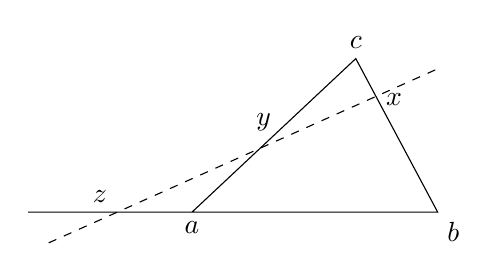
\begin{tikzpicture}[scale=1.3]
      \draw (-1,0)--(3,0)--(2.2, 1.5)--(0.6,0);
      \node[below] at (0.6, 0) {$a$};
      \node[below right] at (3,0) {$b$};
      \node[above] at (2.2, 1.5) {$c$};
      \draw[dashed] (-0.8,-0.3)--(3,1.4);
      \node[above] at (-0.3, 0) {$z$};
      \node[above] at (1.3, 0.7) {$y$};
      \node[right] at (2.4, 1.1) {$x$};
    \end{tikzpicture}\]
    Suppose that they divide these sides in the ratio 
    \[\lambda: 1, \mu: 1, \nu: 1\]
    respectively. Then, the points $x, y, z$ lie on the same line if and only if 
    \[\lambda \mu \nu = -1\]
  \end{corollary}
  \begin{proof}
  By the previous theorem, the points $x, y, z$ are linearly dependent (i.e. lies on a line) if and only if the matrix of barycentric coordinates of $x, y, z$ with respect to $a, b, c$, which is
  \begin{equation}
    \begin{pmatrix}
    0 & \frac{1}{\lambda + 1} & \frac{\lambda}{\lambda + 1} \\
    \frac{\mu}{\mu + 1} & 0 & \frac{1}{\mu + 1} \\
    \frac{1}{\nu + 1} & \frac{\nu}{\nu+1} & 0
    \end{pmatrix}
  \end{equation}
  has nonzero determinant. The determinant of the above matrix is $0$ if and only if $\lambda \mu \nu = -1$. 
  \end{proof}

  \begin{corollary}[Ceva's Theorem]
    In the triangle above, the lines $ax, by, cz$ intersect at one point if and only if 
    \begin{equation}
      \lambda \mu \nu = 1
    \end{equation}
  \end{corollary}
  \begin{proof}
    The proof can be done using barycentric coordinates. 
  \end{proof}

  \begin{theorem}
    A nonempty subset $P \subset S$ is a plane if and only if for any two distinct points $a, b \in P$, the line through $a$ and $b$ also lies in $P$. 
  \end{theorem}

  \begin{theorem}
    Given an inhomogeneous system of linear equations of form 
    \begin{equation}
      A x = b
    \end{equation}
    the set of solutions is an affine plane of dimension $n-r$, where $n$ is the number of variables and $r$ is the rank of the matrix $A$. More precisely, given that the plane is in the form $P = p_0 + U$, $p_0$ is one solution and $U$ is the set of vectors that satisfy the homogeneous system
    \begin{equation}
      Ax = 0
    \end{equation}
  \end{theorem}

  Let us observe the relative position of two planes. 

  \begin{theorem}
    Given two planes 
    \begin{align*}
      P_1 = p_1 + U_1, & P_2 = p_2 + U_2
    \end{align*}
    $P_1$ and $P_2$ intersect if and only if 
    \begin{equation}
      \overline{p_1 p_2} \subset U_1 + U_2
    \end{equation}
    where $U_1 + U_2$ is the set of all vectors of form $u_1 + u_2$, where $u_1 \in U_1, u_2 \in U_2$. 
  \end{theorem}

  Now, consider the class of functions on an affine space corresponding to the class of linear functions on a vector space. 

  \begin{definition}
    An \textbf{affine-linear} function on an affine space $S$ is a function $f: S \longrightarrow \mathbb{F}$ such that
    \begin{equation}
      f(p + x) = f(p) + \alpha (x), \;\; p \in S , x \in V
    \end{equation}
    where $\alpha$, called the \textbf{differential}, is a linear function on the vector space $V$. Let $o \in S$ be a fixed origin. By setting $p = o$, we can express an affine linear function in vectorized form as 
    \begin{equation}
      f(x) = \alpha (x) + b, \;\; b \in \mathbb{F}
    \end{equation}
    where $b = f(o)$. This implies the following coordinate form of $f$. 
    \begin{equation}
      f(x) = b + \sum_i a_i x_i
    \end{equation}
  \end{definition}

  A particular case of affine-linear functions are constant functions, where the defining characteristic is the zero differential. 

  \begin{theorem}
    Given that $\dim{S} = n$, affine-linear functions on $S$ form a $(n+1)$-dimensional subspace on the space of all linear functions on $S$. 
  \end{theorem}

  \begin{theorem}
    Barycentric coordinates are affine-linear functions. 
  \end{theorem}

  \begin{theorem}
    Let $f$ be an affine-linear function. Then
    \begin{equation}
      f \bigg( \sum_i \lambda_i p_i \bigg) = \sum_i \lambda_i f(p_i)
    \end{equation}
    for any barycentric linear combination $\sum_i \lambda_i p_i$ of points $p_1, ..., p_k$. 
  \end{theorem}

  \begin{definition}
    An affine space associated with a Euclidean vector space is called a \textbf{Euclidean affine space}. The \textbf{distance $\rho$} between two points in a Euclidean space is defined as
    \begin{equation}
      \rho(p, q) = ||\overline{pq}||
    \end{equation}
    This definition of $\rho$ satisfies the axioms of a metric space. 
  \end{definition}

\subsection{Convex Sets}

  Let $S$ be an affine space over the field of real numbers and $V$, the associated vector space. 

  \begin{definition}
    The \textbf{(closed) interval} connecting points $p, q \in S$ is the set
    \begin{equation}
      pq = \{\lambda p + (1-\lambda) q \;|\; 0 \leq \lambda \leq 1\}
    \end{equation}
    Geometrically, we can think of this as the straight line segment connecting point $p$ with point $q$. 
  \end{definition}

  \begin{definition}
    A set $M \subset S$ is \textbf{convex} if for any two points $p, q \in S$, it contains the whole interval $p, q$. 
  \end{definition}

  Clearly, the intersection of convex sets is convex. However, the union of them is not. 

  \begin{definition}
    A \textbf{convex linear combination} of points in $S$ is their barycentric linear combination with nonnegative coefficients. 
  \end{definition}

  It is clear to visualize the following theorem. 

  \begin{theorem}
    For any points $p_0, ..., p_k$ in a convex set $M \subset S$, the set $M$ also contains every convex linear combination 
    \begin{equation}
      p = \sum_i \lambda_i p_i
    \end{equation}
    Furthermore, for any set $M \subset S$, the set $\conv{M}$ of all convex linear combinations of points in $M$ is convex. 
  \end{theorem}

  \begin{definition}
    Given $M \subset S$, the set $\conv M$ is the smallest convex set containing $M$. It is called the \textbf{convex hull} of $M$. 
  \end{definition}

  \begin{definition}
    The convex hull of a system of affinely independent points $p_0, p_1, ..., p_n$ in an $n$-dimensional affine space is called the \textbf{$n$-dimensional simplex} with vertices $p_0, ..., p_n$. 
  \end{definition}

  It is clear that the interior points of a simplex is precisely the set of all points whose barycentric coordinates with respect to the vertices are all positive. 

  \begin{example}
    Here are common examples of simplices.
    \begin{enumerate}
      \item A $0$-dimensional simplex is a point. 
      \item A $1$-dimensional simplex is a closed line interval. 
      \item A $2$-dimensional simplex is a triangle. 
      \item A $3$-dimensional simplex is a tetrahedron. 
    \end{enumerate}
  \end{example}

  \begin{theorem}
    A convex set $M$ has interior points if and only if $\aff M = S$. 
  \end{theorem}

  \begin{definition}
    A convex set that has interior points is called a \textbf{convex body}. Clearly, every convex body in $n$-dimensional affine space $S$ is $n$-dimensional. 
  \end{definition}

  The set of interior points of a convex body $M$, denoted $M^\circ$, is an open convex body. 

  \begin{definition}
    For any nonconstant affine-linear function $f$ on the set $S$, let
    \begin{align*}
      H_f \equiv \{p \in S \;|\; f(p) = 0\} \\
      H^+_f \equiv \{p \in S \;|\; f(p) \geq 0\} \\
      H^-_f \equiv \{p \in S \;|\; f(p) \leq 0\}
    \end{align*}
    The set $H_f$ is a hyperplane, and $H^+_f, H^-_f$ are called \textbf{closed half spaces}. 
  \end{definition}

  \begin{definition}
    A hyperplane $H_f$ is a \textbf{supporting hyperplane} of a closed convex body $M$ if $M \subset H^+_f$ and $H_f$ contains at least one (boundary) point of $M$. The half space $H^+_f$ is then called the \textbf{supporting half-space} of $M$. 
  \end{definition}

  \begin{theorem}
    A hyperplane $H$ that passes through a boundary point of a closed convex body $M$, is supporting if and only if $H \cap M^\circ = \emptyset$. 
  \end{theorem}

  A key theorem of convex sets is the following separation theorem. 

  \begin{theorem}[Separation Theorem]
    For every boundary point of a closed convex body, there exists a supporting hyperplane passing through this point. 
  \end{theorem}

  This theorem leads to the following one. 

  \begin{theorem}
    Every closed convex set $M$ is an intersection of (perhaps infinitely many) half-spaces. 
  \end{theorem}

  \begin{definition}
    A \textbf{polyhedron} is the intersection of a finite number of half-spaces. A convex polyhedron which is also a body is called a \textbf{convex solid}. 
  \end{definition}

  \begin{example}
    A simplex with vertices $p_0, p_1, ..., p_n$ is a convex polyhedron since it is determined by linear inequalities $x_i \geq 0$ for $i = 0, 1, ..., n$, where $x_0, x_1, ..., x_n$ are barycentric coordiantes with respect to $p_0, p_1,..., p_n$. 
  \end{example}

  \begin{example}
    A convex polyhedron determined by linear inequalities $0 \leq x_i \leq 1$ for $i = 1, ..., n$, where $x_1,..., x_n$ are affine coordinates with respect ot some frame, is called an $n$-dimensional parallelopiped. 
  \end{example}

  \begin{definition}
    A point $p$ of a convex set $M$ is \textbf{extreme} if it is not an interior point of any interval in $M$. 
  \end{definition}

  \begin{theorem}
    A bounded closed convex set $M$ is the convex hull of the set $E(M)$ of its extreme points. 
  \end{theorem}

  We can create a stronger statement with the following theorem. 

  \begin{theorem}[Minkowski-Weyl Theorem]
    The following properties of a bounded set $M \subset S$ is equivalent.
    \begin{enumerate}
      \item $M$ is a convex polyhedron. 
      \item $M$ is a convex hull of a finite number of points. 
    \end{enumerate}
  \end{theorem}

  \begin{definition}
    A \textbf{face} of a convex polyhedron $M$ is a nonempty intersection of $M$ with some of its supporting hyperplanes. Given that $\dim \aff M = n$, 
    \begin{enumerate}
      \item A $0$-dimensional face is called a \textbf{vertex}. 
      \item A $1$-dimensional face an \textbf{edge}. 
      \item ...
      \item An $(n-1)$-dimensional face a \textbf{hyperface}. 
    \end{enumerate}
  \end{definition}

  Therefore, if a convex polyhedron is determined by a system of linear inequalities, we can obtain its faces by replacing some of these inequalities with equalities (in such a way that we do not get the empty set). 

  The following theorem demonstrates that in order to find its faces, it suffices to consider only the hyperplanes $H_{f_1}, ..., H_{f_m}$. 

  \begin{theorem}
    Every face $\Gamma$ of the polyhedron $M$ is of the form
    \begin{equation}
      \Gamma = M \cap \bigg( \bigcap_{j \in J} H_{f_j} \bigg)
    \end{equation}
    where $J = \{1, 2, ..., m\}$
  \end{theorem}

  \begin{theorem}
    The extreme points of a convex polyhedron $M$ are exactly its vertices. 
  \end{theorem}

  The following theorem is used often in linear programming and in optimization. 

  \begin{theorem}
    The maximum of an affine-linear function on a bounded convex polyhedron $M$ is attained at a vertex. 
  \end{theorem}

\subsection{Affine Transformations and Motions}

  Let $S$ and $S^\prime$ be affine spaces associated with vector spaces $V$ and $V^\prime$, respectively, over the same field $\mathbb{F}$. 

  \begin{definition}
    An \textbf{affine map} from the space $S$ to the space $S^\prime$ is a map $f: S \longrightarrow S^\prime$ such that
    \begin{equation}
      f(p+x) = f(p) + \varphi(x), \;\; p \in S, x \in V
    \end{equation}
    for some linear map $\varphi: V \longrightarrow V^\prime$. It follows that
    \begin{equation}
      \varphi(\overline{pq}) = \overline{f(p) f(q)}, \;\; p, q \in S
    \end{equation}
    Thus, $f$ determines the linear map $\varphi$ uniquely. Similarly, $\varphi$ is called the \textbf{differential} of $f$, denoted $df$. 
  \end{definition}

  \begin{theorem}
    Let $f: S \longrightarrow S^\prime$ and $g: S^\prime \longrightarrow S^{\prime \prime}$ be two affine maps. Then the map
    \begin{equation}
      g \circ f : S \longrightarrow S^{\prime\prime}
    \end{equation}
    is also affine. Also
    \begin{equation}
      d(g \circ f) = dg \cdot df
    \end{equation}
    where $dg$ and $df$ are the differentials of $g$ and $f$, respectively. 
  \end{theorem}

  For $\mathbb{F} = \mathbb{R}$, the differential of an affine map is a particular case of a differential of a smooth map in analysis. That is, the differential is the linear approximation of the function $f$. 

  \begin{theorem}
    An affine map is bijective if and only if its differential is bijective. 
  \end{theorem}

  \begin{definition}
    Similar to linear transformations between vector spaces, bijective affine transformations are called \textbf{isomorphisms} of affine spaces. Affine spaces are \textbf{isomorphic} if there exists an isomorphism between them. 
  \end{definition}

  \begin{corollary}
    Finite-dimensional affine spaces over the same field are isomorphic if and only if they have the same dimension. 
  \end{corollary}

  \begin{definition}
    An affine map from an affine space $S$ to itself is called an \textbf{affine transformation}. Bijective affine transformations form a group called the \textbf{affine group of $S$}, denoted $\GA(S)$. 
  \end{definition}

  It follows that given affine space $S$ with associated vector space $V$, the projection map
  \begin{equation}
    d: \GA(S) \longrightarrow \GL(V)
  \end{equation}
  is a group homomorphism. It's kernel is the group of parallel translations, called Tran$(S)$. 
  \begin{equation}
    t_a : p \mapsto p + a, \;\; a \in V
  \end{equation}

  \begin{theorem}
    For any $f \in \GA(S)$ and $a \in V$, 
    \begin{equation}
      f t_a f^{-1} = t_{df(a)}
    \end{equation}
  \end{theorem}

  \begin{definition}
    A \textbf{homothety} with the center $o$ and coefficient $\lambda$ is an affine transformation defined as
    \begin{equation}
      f( o + x ) \equiv o + \lambda x
    \end{equation}
    In its vectorized form, it is expressed
    \begin{equation}
      f(x) = \lambda x + b, \;\; b \in V
    \end{equation}
    A homothety with coefficient $-1$ is called a \textbf{central symmetry}. 
  \end{definition}

  The group of affine transformations determines the \textbf{affine geometry} of the space. The following theorem shows that all simplices are equal in affine geometry. 

  \begin{theorem}
    Let $\{p_0, ..., p_n\}$ and $\{q_0, ..., q_n\}$ be two systems of affinely independent points in an $n$-dimensional affine space $S$. Then there exists a unique affine transformation $f$ that maps $p_i$ to $q_i$ for $i = 0, 1, ..., n$. 
  \end{theorem}
  \begin{proof}
    It is easy to see once we realize that there exists a unique linear map $\varphi$ of the space $V$ that maps the basis $\{\overline{p_0 p_1}, ..., \overline{p_0 p_n}\}$ to the basis $\{\overline{q_0 q_1}, ..., \overline{q_0 q_n}\}$. If we vectorize $S$ by taking $p_0$ as the origin, the affine transformation in question has the form 
    \begin{equation}
      f(x) = \varphi(x) + \overline{p_0 q_0}
    \end{equation}
  \end{proof}

  \begin{corollary}
    In real affine geometry all parallelopipeds are equal. 
  \end{corollary}

  \begin{definition}
    A \textbf{motion} of the space $S$ is an affine transformation of $S$ whose differential is an orthogonal operator (i.e. an origin preserving isometry). Every motion is bijective. 
  \end{definition}

  Motions of a Euclidean space $S$ form a group denoted Isom$\,S$. A motion is called \textbf{proper (orientation preserving)} if its differential belongs to SO$(V)$ and improper otherwise. 

  \begin{lemma}
    The group Isom$\,S$ is generated by reflections through hyperplanes. 
  \end{lemma}

  \begin{definition}
    Let $M$ be a solid convex polyhedron in an $n$-dimensional Euclidean space. A \textbf{flag of $M$} is a collection of its faces $\{F_0, F_1, ..., F_{n-1}\}$ where $\dim{F_k} = k$ and $F_0 \subset F_1 \subset ... \subset F_{n-1}$. 
  \end{definition}

  \begin{definition}
    A convex polyhedron $M$ is \textbf{regular} if for any two of its flags, there exists a motion $f \in$ Sym$\,M$ mapping the first to the second, where 
    \begin{equation}
      \text{Sym}\,M \equiv \{f \in \text{Isom}\,S \;|\; f(M) = M \}
    \end{equation}
  \end{definition}

  Two dimensional regular polyhedra are the ordinary \textbf{regular polygons}. Their symmetry groups are known as the dihedral groups.

  Three dimensional regular polyhedra are \textbf{Platonic solids}, which are the regular tetrahedron, cube, octahedron, dodecahedron, and icosahedron. 

  \begin{definition}
    A real vector space $V$ with a fixed symmetric bilinear function $\alpha$ of signature $(k, l)$, where $k, l > 0$ and $\dim{V} = k+l$, is called the \textbf{pseudo-Euclidean vector space} of signature $(k, l)$. The group of $\alpha$-preserving linear transformations of $V$ is called the \textbf{pseudo-orthogonal group} and is denoted O$(V, \alpha)$. In an orthonormal basis, the corresponding matrix group is denoted $O{k,l}$. 
  \end{definition}

\subsection{Quadrics}

  Planes are the simplest objects of affine and Euclidean geometry, which are determined by systems of linear equations. The second simplest are quadratic functions. These types of objects are studied futher in algebraic geometry. 

  \begin{definition}
    An \textbf{affine-quadratic function} on an affine space $S$ is a function $Q: S \longrightarrow \mathbb{F}$ such that its vectorized form is
    \begin{equation}
      Q(x) = q(x) + l(x) + c
    \end{equation}
    for a quadratic function $q$, linear function $l$, and constant $c$. 
  \end{definition}

\subsection{Projective Spaces}

  \begin{definition}
    An $n$-dimensional \textbf{projective space $PV$} over a field $\mathbb{F}$ is the set of one-dimensional subspaces of an $(n+1)$-dimensional vector space $V$ over $\mathbb{F}$. For every $(k+1)$-dimensional subspace $U \subset V$, the subset $PU \subset PV$ is called a $k$-dimensional \textbf{plane} of the space $PV$. 
    \begin{enumerate}
      \item $0$-dimensional planes are the points of $PV$. 
      \item $1$-dimensional planes are called \textbf{lines}
      \item ...
      \item $(n-1)$-dimensional planes are called \textbf{hyperplanes}
    \end{enumerate}
  \end{definition}

  \begin{definition}
    $\mathbb{RP}^1$ is called the real projective line, which is topologically equivalent to a circle. 
  \end{definition}

  \begin{example}
    The real projective space of $\mathbb{R}^2$ is the set of all lines that pass through the origin. It is denoted $\mathbb{R P}^2$ and called the \textbf{real projective plane}. 
  \end{example}

  \begin{example}
    $\mathbb{RP}^3$ is diffeomorphic to SO$(3)$. 
  \end{example}

  \begin{example}
    The space $\mathbb{RP}^n$ is formed by taking the quotient of $\mathbb{R}^{n+1} \setminus \{0\}$ under the equivalence relation 
    \begin{equation}
      x \sim \lambda x \text{ for all real numbers } \lambda \neq 0
    \end{equation}
    The set of these equivalence classes is isomorphic to $\mathbb{RP}^n$. 
  \end{example}


\section{Representations}

  We will assume that $V$ is a finite-dimensional vector space over field $\mathbb{C}$. 

  \begin{definition}
    The \textbf{general linear group} of vector space $V$, denoted $\GL(V)$, is the group of all automorphisms of $V$ to itself. The \textbf{special linear group} of vector space $V$, denoted $\SL(V)$ is the subgroup of automorphisms of $V$ with determinant $1$. 
  \end{definition}

  When studying an abstract set, it is often useful to consider the set of all maps from this abstract set to a well known set (e.g. $\GL(V)$). 

  \begin{definition}
    A \textbf{representation} of an (algebraic) group $\mathcal{G}$ is a homomorphism 
    \begin{equation}
      \rho: G \longrightarrow \GL(V)
    \end{equation}
    for some vector space $V$. That is, given an element $g \in \mathcal{G}$, $\rho(g) \in \GL (V)$, meaning that $\rho(g)(v) \in V$. Additionally, since it is a homomorphism, the algebraic structure is preserved. 
    \begin{equation}
      \rho(g_1 \cdot g_2) = \rho(g_1) \cdot \rho(g_2)
    \end{equation}
    where $\cdot$ on the left hand side is the abstract group multiplication while the $\cdot$ on the right hand side is matrix multiplication. To shorten the notation, we will denote 
    \begin{equation}
      g v = \rho(g) v, \; v \in V
    \end{equation}
    Since $\rho$ is a group morphism, we have 
    \begin{equation}
      g_2 (g_1 v) = (g_2 g_1) v \; \iff \rho(g_2) \big( \rho(g_1) (v) \big) = \big( \rho(g_2) \rho(g_1) \big) (v)
    \end{equation}
    Additionally, since $g$ (that is, $\rho(g)$) is a linear map, 
    \begin{equation}
      g(\lambda_1 v_1 + \lambda_2 v_2) = \lambda_1 g v_1 + \lambda_2 g v_2
    \end{equation}
    Usually, we refer to the map as the representation, but if the map is well-understood, we just call the vector space $V$ the representation and say that the group acts on this vector space. 
  \end{definition}

  \begin{example}
    The group $\GL(2, \mathbb{C})$ can be represented a by the vector space $\mathbb{C}^2$, or explicitly, by the group of $2 \times 2$ matrices over $\mathbb{C}$ with nonzero determinant.
    \begin{equation}
      \GL(2, \mathbb{C}) \xmapsto{id} \text{Mat}(2, \mathbb{C})
    \end{equation}
    This is a trivial representation. 
  \end{example}

  We now show a nontrivial representation of $\GL(2, \mathbb{C})$. 

  \begin{example}
    We take Sym$^2 \mathbb{C}^2$, the second symmetric power of $\mathbb{C}^2$. Note that given a basis $x_1, x_2 \in \mathbb{C}^2$, the set
    \begin{equation}
      \{x_1 \odot x_1, x_1 \odot x_2, x_2 \odot x_2\}
    \end{equation}
    forms a basis of Sym$^2 \mathbb{C}^2 \implies \dim\,$Sym$^2 \mathbb{C}^2 = 3$. So, we want to represent $\GL(2, \mathbb{C})$ by associating its element with elements of $\GL(Sym^2 \mathbb{C}^2)$. More concretely, we are choosing to represent a $2 \times 2$ matrix over $\mathbb{C}$ with a $3 \times 3$ matrix group (since $\GL(Sym^2 \mathbb{C}^2) \simeq \GL(3, \mathbb{C})$. Clearly,
    \begin{align*}
      & \rho(g) (x_1 \odot x_1) = g(x_1) \odot g(x_1) \in Sym^2 \mathbb{C}^2 \\
      & \rho(g) (x_1 \odot x_2) = g(x_1) \odot g(x_2) \\
      & \rho(g) (x_2 \odot x_2) = g(x_2) \odot g(x_2)
    \end{align*}
    To present this in matrix form, let us have an element in $\GL (2, \mathbb{C})$
    \begin{equation}
      \mathcal{A} \equiv \begin{pmatrix}
      a & b \\
      c & d
      \end{pmatrix}
    \end{equation}
    We evaluate the corresponding representation in $\GL( Sym^2 \mathbb{C}^2)$. Using the identities above, we have 
    \begin{align*}
      \rho(g) (x_1 \odot x_1) & = g(x_1) \odot g(x_1) \\
      & = (a x_1 + c x_2) \odot (a x_1 + c x_2) \\
      & = a^2 x_1 \odot x_1 + 2ac x_1 \odot x_2 + c^2 x_2 \odot x_2 \\
      \rho(g) (x_1 \odot x_2) & = g(x_1) \odot g(x_2) \\
      & = (a x_1 + c x_2) \odot (b x_1 + d x_2) \\
      & = ab x_1 \odot x_1 + (ad + bc) x_1 \odot x_2 + cd x_2 \odot x_2 \\
      \rho(g) (x_2 \odot x_2) & = g(x_2) \odot g(x_2) \\
      & = (b x_1 + d x_2) \odot (b x_1 + d x_2) \\
      & = b^2 x_1 \odot x_1 + 2bd x_1 \odot x_2 + d^2 x_2 \odot x_2
    \end{align*}
    And this completely determines the matrix. So, 
    \begin{equation}
      \rho \begin{pmatrix}
      a&b\\c&d
      \end{pmatrix} = \begin{pmatrix}
      a^2&ab&b^2\\2ac&ad+bc&2bd\\c^2&cd&d^2
      \end{pmatrix}
    \end{equation}
    is the $3 \times 3$ representation of $\mathcal{A}$ in $\GL(Sym^2 \mathbb{C}^2)$. 
  \end{example}

  We continue to define maps between two representations of $\mathcal{G}$. 

  \begin{definition}
    A \textbf{morphism} between 2 representations 
    \begin{align*}
      & \rho_1: \mathcal{G} \longrightarrow \GL(V_1) \\
      & \rho_2: \mathcal{G} \longrightarrow \GL(V_2) 
    \end{align*}
    of some group but not necessarily the same vector space is a linear map $f: V_1 \longrightarrow V_2$ that is \textbf{compatible} with the group action. That is, $f$ satisfies the property that for all $g \in \mathcal{G}$
    \begin{equation}
      f \circ g = g \circ f
    \end{equation}
    Again, we use the shorthand notation that $g = \rho(g)$, meaning that the statement above really translates to $ f \circ \rho(g) = \rho(g) \circ f$. This is equivalent to saying that the following diagram commutes. 
    \[\begin{tikzcd}
    V_1 \arrow{r}{\rho_1(g)} \arrow{d}{f} & V_1 \arrow{d}{f} \\
    V_2 \arrow{r}{\rho_2 (g)} & V_2
    \end{tikzcd}\]
  \end{definition}

  \begin{definition}
    Let $V$ be a representation of $\mathcal{G}$. A \textbf{subrepresentation} is a subspace $W \subset V$ such that for all $g \in \mathcal{G}$ and for all $w \in W$, 
    \begin{equation}
      \rho(g)(w) \in W
    \end{equation}
  \end{definition}

  \begin{example}
    $V$ and $\{0\}$ are always subrepresentations of $V$. 
  \end{example}

  We now introduce the "building blocks" of all representations. 
  \begin{definition}
    A representation $W$ is \textbf{irreducible representation} if $\{0\}$ and $W$ are the only subrepresentations of $W$. 
  \end{definition}

  \begin{lemma}[Schur's Lemma]
    Let $V_1, V_2$ be irreducible representations and let $f: V_1 \longrightarrow V_2$ be a morphism (of representations). Then, either
    \begin{enumerate}
      \item $f$ is an isomorphism. 
      \item $f = 0$
    \end{enumerate}
    Furthermore, any 2 isomorphisms differ by a constant. That is, 
    \begin{equation}
      f_1 = \lambda f_2
    \end{equation}
  \end{lemma}
  \begin{proof}
    $\ker{f}$ is clearly a vector space. Furthermore, it is a subrepresentation (since it is a subspace of $V_1$) $\implies \ker{f} = V$ or $\ker{f} = 0$. If $\ker{f} = V$, then $f = 0$ and the theorem is satisfied. If $\ker{f} = 0$, then $f$ is injective, and $\im{f}$ is a subrepresentation of $V_2 \implies \im{f} = 0$ or $\im{f} = V_2$. But $\im{f} \neq 0$ since $f$ is injective, so $\im{f} = V_2 \implies f$ is surjective $\implies f$ is bijective, that is, $f$ is an isomorphism of vector spaces. So, the inverse $f^{-1}$ exists, and this map $f^{-1}$ satisfies
    \begin{equation}
      f^{-1} \circ \rho_2(g) = \rho_1 (g) \circ f^{-1}
    \end{equation}
    To prove the second part, without loss of generality, assume that the first isomorphism is the identity mapping. That is, 
    \begin{equation}
      f_1 = id
    \end{equation}
    Since we are working over the field $\mathbb{C}$, we can find an eigenvector of $f_2$. That is, there exists a $v \in V_1$ such that 
    \begin{equation}
      f_2 (v) = \lambda v
    \end{equation}
    Now, we define the map
    \begin{equation}
      f: V_1 \longrightarrow V_2, \; f \equiv f_2 - \lambda f_1
    \end{equation}
    Clearly, $\ker{f} \neq 0$, since $v \in \ker{f}$. That is, we have a map $f$ between 2 irreducible representations that has a nontrivial kernel. This means that $f = 0 \implies f_2 = \lambda f_1$.  
  \end{proof}

  \begin{theorem}[Mache's Theorem]
    Let $V$ be finite dimensional, with $\mathcal{G}$ a finite group. Then, $V$ can be decomposed as 
    \begin{equation}
      V = \bigoplus_{i} V_i
    \end{equation}
    where each $V_i$ is an irreducible representation of $\mathcal{G}$. 
  \end{theorem}
  \begin{proof}
    By induction on dimension, it suffices to prove that if $W$ is a subrepresentation of $V$, then there exists a subrepresentation $W^\prime \subset V$ such that $W \oplus W^\prime = V$. So, if $V$ isn't an irreducible representation, it can always be decomposed into smaller subrepresentations $W$ and $W^\prime$ that direct sum to $V$. Now, we define the canonical (linear) projection 
    \begin{equation}
      \pi: V \longrightarrow W
    \end{equation}
    Then, we define the new map 
    \begin{equation}
      \Tilde{\pi}: V \longrightarrow W, \; \Tilde{\pi}(v) \equiv \frac{1}{|\mathcal{G}|} \sum_{g \in \mathcal{G}} \rho(g)\big|_W \circ \pi \circ \rho(g)^{-1}
    \end{equation}
    This "averaging" of the group elements are done so that this mapping is a map of representations. This implies that 
    \begin{equation}
      V = W \oplus \ker{\Tilde{\pi}}
    \end{equation}
    meaning that $V$ can indeed be decomposed into direct sums of subrepresentations. 
  \end{proof}


\section{Lie Groups and Lie Algebras}

  \begin{definition}
    A \textbf{Lie group} is a group $\mathcal{G}$ that is also a finite-dimensional smooth manifold, in which the group operations of multiplication and inversion are smooth maps. Smoothness of the group multiplication
    \begin{equation}
      \mu: \mathcal{G} \times \mathcal{G} \longrightarrow \mathcal{G}, \; \mu(x, y) = x y
    \end{equation}
    means that $\mu$ is a smooth mapping of the product manifold $\mathcal{G} \times \mathcal{G}$ into $\mathcal{G}$. These two requirements can be combined to the single requirement that tahe mapping 
    \begin{equation}
      (x, y) \mapsto x^{-1} y
    \end{equation}
    be a smooth mapping of the product manifold into $\mathcal{G}$. 
  \end{definition}

  \begin{definition}
    A \textbf{Lie Algebra} is a vector space $\mathfrak{g}$ with an operation called the \textbf{Lie Bracket} 
    \begin{equation}
      [\cdot, \cdot]: \mathfrak{g} \times \mathfrak{g} \longrightarrow \mathfrak{g}
    \end{equation}
    Satisfying
    \begin{enumerate}
      \item Bilinearity: $[ax + by, z] = a[x,z] + b[y,z], \; [z, ax + by] = a[z, x] + b[z,y]$
      \item Anticommutativity: $[x,y] = -[y,x]$
      \item Jacobi Identity: $[x,[y,z]] + [y,[z,x]] + [z,[x,y]] = 0$
    \end{enumerate}
    Clearly, this implies that $\mathfrak{g}$ is a nonassociative algebra. Note that a Lie Algebra does not necessarily need to be an algebra in the sense that there needs to be multiplication operation that is closed in $\mathfrak{g}$. 
  \end{definition}

  \begin{example}
    A common example of a Lie Braket in the algebra of matrices is defined
    \begin{equation}
      [A, B] \equiv AB - BA
    \end{equation}
    called the \textbf{commutator}. Note that in this case, the definition of the Lie bracket is dependent on the definition of the matrix multiplication. Without defining the multiplication operation, we wouldn't know what $AB$ or $BA$ means. Therefore, we see that the Lie algebra of $n \times n$ matrices has three operations: matrix addition, matrix multiplication, and the commutator (along with scalar multiplication). But in general, it is not necessary to have that multiplication operation for abstract Lie algebras. $\mathfrak{g}$ just needs to be a vector space with the bracket.  
  \end{example}

  \begin{example}
    The set of all symmetric matrices is a vector space, but it is \textbf{not} a Lie algebra since the commutator $[A,B]$ is not symmetric unless $A B = B A$. 
  \end{example}

  We will first talk about groups of matrices as a more concerete example before we get into abstract Lie groups. Recall that the matrix exponential map is defined
  \begin{equation}
    exp: \text{Mat}(n, \mathbb{C}) \longrightarrow \text{mat}(n, \mathbb{C}), \; exp(A) = e^A = \sum_{p \geq 0} \frac{A^p}{p!}
  \end{equation}
  Note that this value is always well defined. This lets us define
  \begin{equation}
    exp(t A) \equiv e^{t A} \equiv I + tA + \frac{1}{2} t^2 A^2 + \frac{1}{3!} t^3 A^3 + ... 
  \end{equation}
  where if $t$ is small, we can expect a convergence. Note that exp maps addition to multiplication. That is, we can interpret it as a homomorphism from 
  \begin{equation}
    exp: \mathfrak{g} \longrightarrow \mathcal{G}
  \end{equation}
  where $\mathfrak{g}$ is the Lie algebra and $\mathcal{G}$ is the Lie group (which we will treat just as a matrix group). To find the inverse of the exponential map, we can take the derivative of $e^{tA}$ at $t=0$. That is, 
  \begin{align*}
    \bigg(\frac{d}{d t} e^{tA} \bigg) \bigg|_{t=0} & = \bigg(\sum_{k=0}^\infty \frac{1}{k!} t^k A^{k+1} \bigg) \bigg|_{t=0} = A
  \end{align*}
  So, the mapping
  \begin{equation}
    \frac{d}{dt} \bigg|_{t=0}: \mathcal{G} \longrightarrow \mathfrak{g}
  \end{equation}
  maps the Lie group back to the algebra. We can interpret this above mapping by visualizing the Lie Algebra as a tangent (vector) space of the abstract Lie group $\mathcal{G}$ at the identity element of the Lie group. The visualization below isn't the most abstract one, but it may help:
  \begin{center}
    \includegraphics[scale=0.2]{img/Lie_Algebra_Tangent_Space.PNG}
  \end{center}
  For example, say that the Lie group $\mathcal{G}$ is a unit circle in $\mathbb{C}$, then the Lie algebra of $\mathcal{G}$ is the tangent space at the identity $1$, which can be identified as the imaginary line in the complex plane $\{i t \; | \; t \in \mathbb{R}\}$, with 
  \begin{equation}
    i t \mapsto exp(it) \equiv e^{it} \equiv \cos{t} + i \sin{t}
  \end{equation}

  \begin{center}
    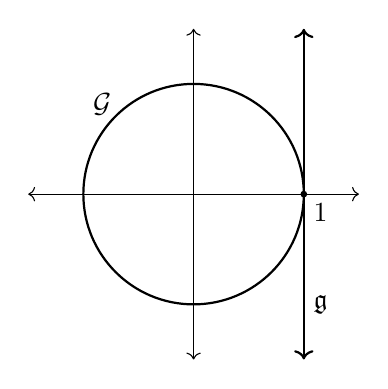
\begin{tikzpicture}[scale=0.7]
      \draw[thick] (0,0) circle (2);
      \node[below right] at (-2,2) {$\mathcal{G}$};
      \draw[<->] (-3,0)--(3,0);
      \draw[<->] (0,-3)--(0,3);
      \draw[fill] (2,0) circle (0.05);
      \node[below right] at (2,0) {$1$};
      \draw[thick, <->] (2,-3)--(2,3);
      \node[right] at (2,-2) {$\mathfrak{g}$};
    \end{tikzpicture}
  \end{center}
  So, analyzing the Lie group by looking at its Lie algebra turns a nonlinear problem to a linear one; this is called a \textbf{linearization} of the Lie group. The existence of this exponential map is one of the primary reasons that Lie algebras are useful for studying Lie groups. 

  \begin{example}
    The exponential map 
    \begin{equation}
      exp: \mathbb{R} \longrightarrow \mathbb{R}^+, \; x \mapsto e^x
    \end{equation}
    is a group homomorphism that maps $(\mathbb{R}, +)$ to $(\mathbb{R}^+, \times)$. This means that $\mathbb{R}$ is the Lie algebra of the Lie group $\mathbb{R}^+$. 
  \end{example}

  \begin{theorem}
    If $A$ and $B$ are commuting square matrices, then 
    \begin{equation}
      e^{A + B} = e^A \, e^B
    \end{equation}
    In general, the solution $C$ to the equation
    \begin{equation}
      e^{A} \, e^B = e^C
    \end{equation}
    is given by the \textbf{Baker-Campbell-Hausdorff formula}, defined
    \begin{equation}
      C = A + B + \frac{1}{2}[A,B] + \frac{1}{12} [A,[A,B]] - \frac{1}{12} [B,[A,B]] + ...
    \end{equation}
    consisting of terms involving higher commutators of $A$ and $B$. The full series is much too complicated to write, so we ask the reader to be satisfied with what is shown. 
  \end{theorem}

  The BCH formula is messy, but it allows us to compute products in the Lie Group as long as we known the commutators in the Lie Algebra. 

  Therefore, we can describe the process of constructing a Lie group from a Lie Algebra (which a vector space) as such. We take a vector space $V$ and endow it the additional bracket operation. We denote this as
  \begin{equation}
    \mathfrak{g} \equiv (V, [\cdot, \cdot])
  \end{equation}
  Then, we take every element of $\mathfrak{g}$ and apply the exponential map to them to get an another set $\mathcal{G}$. We then endow a group structure on $\mathcal{G}$ by defining the multiplication as 
  \begin{equation}
    \cdot: \mathcal{G} \times \mathcal{G} \longrightarrow \mathcal{G}, \; e^A \cdot e^B = e^{A * B}
  \end{equation}
  where $A*B$ is defined by the BCH formula up to a certain $k$th order. Since the $*$ operation is completely defined by the bracket in the Lie algebra, it tells us how to multiply in the Lie group. This process can be made more abstractly, depending on what $A, B$ and $[\cdot,\cdot]$ is, beyond matrices. 

\subsection{Lie Algebras of Classical Lie Groups}

  \begin{definition}
    The \textbf{general linear group} of vector space $V$ is the group of all automorphisms of $V$, denoted $\GL(V)$. Additionally, $\GL(n, \mathbb{R})$ is the group of real $n \times n$ matrices with nonzero determinant, and $\SL(n, \mathbb{R})$ is the group of real $n \times n$ matrices with determinant $= 1$.
  \end{definition}

  \subsubsection[Lie Algebras of SL(2, R) and SL(2, C)]{Lie Algebras of $\SL(2, \mathbb{R})$ and $\SL(2, \mathbb{C})$}

    Given the group $\SL(2, \mathbb{R})$, there must be a corresponding Lie algebra of matrices such that $g = e^A \in \SL(2, \mathbb{R})$. We attempt to find this Lie algebra. Let $g \in \SL(2, \mathbb{R})$, with $g = e^A$. So, if $\det{g} = 1$, what is the corresponding restriction on $A$ in the algebra? We use the following proposition. 

    \begin{proposition}
      \begin{equation}
        \det{(e^A)} = e^{\Tr{(A)}}
      \end{equation}
    \end{proposition}
    \begin{proof}
      Put $A$ in Jordan Normal Form: $A = S^{-1} J S \implies A^n = S^{-1} J^n S \implies exp(A) = S^{-1} exp(A) S \implies \det{(exp(A))} = \det{e^J}$. But since $J$ is upper trianglar, $J^n$ is upper triangular $\implies e^J$ is upper triangular, which implies that 
      \begin{equation}
        \det{e^J} = \prod_i e^{\lambda_i} = e^{\Tr{(J)}} = e^{\Tr{(A)}}
      \end{equation}
      since trace is invariant under a change of basis. 
    \end{proof}

    So, $\det{(e^A)} = 1 \implies \Tr{(A)} = 2 \pi i n$ for $n \in \mathbb{Z}$. Since we want to component connected to the identity, we choose $n=0$ meaning that $\Tr{(A)} = 0$. And we are done. That is, the Lie algebra of $\SL(2, \mathbb{R})$ consists of traceless $2 \times 2$ matrices, denoted $\mathfrak{sl}_2 \mathbb{R}$. $\mathfrak{sl}_2 \mathbb{R}$ has basis (chosen arbitrarily) 
    \begin{equation}
      \bigg\{ H = \begin{pmatrix}
      1&0\\0&-1
      \end{pmatrix}, X = \begin{pmatrix}
      0&1\\0&0
      \end{pmatrix}, Y = \begin{pmatrix}
      0&0\\1&0
      \end{pmatrix}\bigg\}
    \end{equation}
    and the identity in the Lie algebra is the zero matrix, which translates to the $2 \times 2$ identity matrix in the Lie group. 
    \begin{equation}
      exp \begin{pmatrix}
      0&0\\0&0
      \end{pmatrix} = I
    \end{equation}
    We must not forget to define the bracket structure in $\mathfrak{sl}_2 \mathbb{R}$, so we define it as the commutator, which gives the identity
    \begin{align*}
      & [H,X] = HX - XH = 2X \\
      & [H,Y] = HY - YH = -2Y \\
      & [X,Y] = XY - YX = H
    \end{align*}
    Note that regular matrix multiplication is not closed within this Lie algebra. For example, 
    \begin{equation}
      X Y = \begin{pmatrix}
      1&0\\0&0
      \end{pmatrix}
    \end{equation}
    is clearly not traceless. However, the bracket operation keeps the matrices within this traceless condition (and thus, within this algebra), so you can't just stupidly multiply matrices together in a Lie algebra. Remember that regular matrix multiplication does not have anything to do with the Lie bracket and does not apply to this group. This algebra also simplifies the multiplicative inverse of a group to a simple additive inverse, making calculations easier. 

    Similarly, the Lie algebra of $\SL(2, \mathbb{C})$ also has the same basis 
    \begin{equation}
      \bigg\{ H = \begin{pmatrix}
      1&0\\0&-1
      \end{pmatrix}, X = \begin{pmatrix}
      0&1\\0&0
      \end{pmatrix}, Y = \begin{pmatrix}
      0&0\\1&0
      \end{pmatrix}\bigg\}
    \end{equation}
    but we choose the field to be $\mathbb{C}$, meaning that we take complex linear combinations rather than real linear ones. 

  \subsubsection[Lie Algebra of SU(2)]{Lie Algebra of \(\SU(2)\)}

    $g \in $ SU$(2) \implies \det{g} = 1 \implies \Tr{A} = 0$. We also see that by definition $e^A$, 
    \begin{equation}
      (e^A)^\dagger = e^{A^\dagger} \text{ and } (e^A)^{-1} = e^{-A}
    \end{equation}
    which implies that $A^\dagger = - A$. That is, the unitary condition implies that the Lie algebra elements in $\mathfrak{su}(2)$ are traceless, anti-self adjoint $2 \times 2$ matrices over $\mathbb{C}$. 

    \begin{definition}
      The \textbf{Pauli matrices} are the three matrices
      \begin{equation}
        \bigg\{ \sigma_x = \begin{pmatrix}
        0&1\\1&0
        \end{pmatrix}, \sigma_y = \begin{pmatrix}
        0&-i\\i&0
        \end{pmatrix}, \sigma_z = \begin{pmatrix}
        1&0\\0&-1
        \end{pmatrix}\bigg\}
      \end{equation}
      Note that with some calculation, 
      \begin{align*}
        & [\sigma_x, \sigma_y] = 2 i \sigma_z \\
        & [\sigma_y, \sigma_z] = 2 i \sigma_x \\
        & [\sigma_z, \sigma_x] = 2 i \sigma_y
      \end{align*}
    \end{definition}

    To identify the basis of $\mathfrak{su}(2)$, we take the Pauli matrices and let 
    \begin{align*}
      & A_x \equiv - \frac{i}{2} \sigma_x = \begin{pmatrix} 0&-i/2\\-i/2&0 \end{pmatrix} \\
      & A_y \equiv - \frac{i}{2} \sigma_y = \begin{pmatrix}0&-1/2\\1/2&0\end{pmatrix} \\
      & A_z \equiv -\frac{i}{2} \sigma_z = \begin{pmatrix}-i/2&0\\0&i/2\end{pmatrix}
    \end{align*} 
    be the basis of $\mathfrak{su}(2)$. Clearly, $A_x, A_y, A_z$ are all traceless, anti-self adjoint $2 \times 2$ matrices. Moreover, they also satisfy
    \begin{align*}
      & [A_x, A_y] = A_z \\
      & [A_y, A_z] = A_x \\
      & [A_z, A_x] = A_y
    \end{align*}
    However, note that the algebra $\mathfrak{su}(2)$ consists of all \textbf{real} linear combinations of $A_x, A_y, A_z$. That is, $\mathfrak{su}(2)$ is a 3 dimensional \textbf{real} vector space, even though it has basis elements containing complex numbers. 

    However, we can always complexify this space by simply replacing real scalar multiplication in $\mathfrak{su}(2)$ with complex scalar multiplication. By complexifying $\mathfrak{su}(2)$, the Lie group SU$(2)$ formed by taking the exponential map on this complexified space is actually identical to $\SL(2, \mathbb{C})$. Indeed, this is true because first, the basis $\{H, X, Y\}$ of $\mathfrak{sl}_2 \mathbb{C}$ and the basis $\{A_x, A_y, A_z\}$ of $\mathfrak{su}(2)$ span precisely the same subspace in the vector space Mat$(2, \mathbb{C})$, meaning that the two Lie algebras are the same vector space. Secondly, the bracket operation $[\cdot, \cdot]$ in both $\mathfrak{sl}_2 \mathbb{C}$ and $\mathfrak{su}(2)$ are equivalent since the operation defined to be the commutator in both cases, resulting in the similarities in the bracket behaviors. 
    \begin{align*}
      [H,X] = 2X & \iff [A_x, A_y] = A_z \\
      [H,Y] = - 2Y & \iff [A_y, A_z] = A_x\\
      [X,Y] = H & \iff  [A_z, A_x] = A_y 
    \end{align*}
    Therefore, the complexification of SU$(2)$ and $\SL(2, \mathbb{R})$ both leads to the construction of $\SL(2, \mathbb{C})$. 

    \begin{center}
      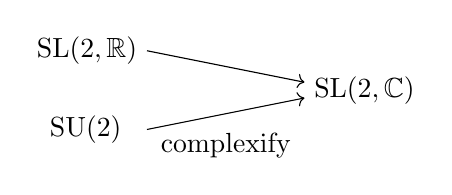
\begin{tikzpicture}
        \node[left] at (0,0.5) {$\SL(2, \mathbb{R})$};
        \node[left] at (-0.2,-0.5) {SU$(2)$};
        \node[right] at (2,0) {$\SL(2,\mathbb{C})$};
        \draw[->] (0,0.5)--(2,0.1);
        \draw[->] (0,-0.5)--(2,-0.1);
        \node at (1,-0.7) {complexify};
      \end{tikzpicture}
    \end{center}
    We can interpret the "real forms" of $\SL(2, \mathbb{C})$ as "slices" of some complex group. However, this does not mean that the real version of these groups are equal. That is, 
    \begin{equation}
      \SL(2, \mathbb{R}) \neq \text{SU}(2)
    \end{equation}

  \subsubsection{Lie Algebra of SO(3)}

    It is easy to see that for SO$(2)$, it is easy to see that its Lie algebra $\mathfrak{so}(2)$ has 
    \begin{equation}
      \bigg\{ \begin{pmatrix}
      0&-1\\1&0
      \end{pmatrix}\bigg\}
    \end{equation}
    as its only basis, since 
    \begin{equation}
      exp  \bigg( \begin{pmatrix}
      0&-1\\1&0
      \end{pmatrix} \theta \bigg) = \begin{pmatrix}
      \cos{\theta} & - \sin{\theta} \\
      \sin{\theta} & \cos{\theta}
      \end{pmatrix}
    \end{equation}
    meaning that the dimension of SO$(2)$ is $1$. By adding a component, we can get a rotation in $\mathbb{R}^3$. 
    \begin{align*}
      & R_x = \begin{pmatrix}0&0&0\\0&0&-1\\0&1&0\end{pmatrix} \implies e^{R_x} = \begin{pmatrix}
      1&0&0\\ 0&\cos{\theta}&-\sin{\theta}\\0&\sin{\theta}&\cos{\theta}
      \end{pmatrix}\\
      & R_y = \begin{pmatrix}0&0&1\\0&0&0\\-1&0&0\end{pmatrix} \implies e^{R_y} = \begin{pmatrix}
      \cos{\theta} & 0 & -\sin{\theta}\\ 0&1&0 \\
      \sin{\theta}& 0 & \cos{\theta} \end{pmatrix} \\
      & R_z = \begin{pmatrix}0&-1&0\\1&0&0\\0&0&0\end{pmatrix} \implies e^{R_z} = \begin{pmatrix}
      \cos{\theta} & -\sin{\theta} & 0\\
      \sin{\theta}& \cos{\theta} & 0 \\ 0 & 0 & 1\end{pmatrix}
    \end{align*}
    That is, $e^{R_x}, e^{R_y}$, and $e^{R_z}$ generates a rotation around the $x, y$, and $z$ axis, respectively, which completely generates the group SO$(3)$. Therefore, the Lie algebra $\mathfrak{so}(3)$ consists of the basis 
    \begin{equation}
      \{R_x, R_y, R_z\}
    \end{equation}
    The bracket structure (again, defined as the commutator) of this Lie algebra is 
    \begin{align*}
      & [R_x, R_y] = R_z \\
      & [R_y, R_z] = R_x \\
      & [R_z, R_x] = R_y
    \end{align*}
    which is similar to the brakcet structure of $\mathfrak{su}(2)$. Therefore, SO$(3)$ and SU$(2)$ have the \textbf{same} Lie algebra, which is the algebra of dimension 3 with the same bracket structure. Note that Lie algebras are uniquely determined by the bracket structure and dimension. However, having the same Lie algebra does not imply that the groups are identical (obviously) nor isomorphic. For example, 
    \begin{equation}
      exp(2\pi R_z) = \begin{pmatrix}
      \cos{2\pi} & -\sin{2\pi} & 0 \\
      \sin{2\pi} & \cos{2\pi} & 0 \\
      0 & 0 & 1
      \end{pmatrix} = I
    \end{equation}
    while 
    \begin{equation}
      exp(2\pi A_z) = 
      exp(-i \pi \sigma_z) = exp \bigg(-i \pi \begin{pmatrix}
      1&0\\0&-1
      \end{pmatrix} \bigg) = -I
    \end{equation}
    There is discrepancy by a factor of $-1$. In fact, it turns out that
    \begin{equation}
      \text{SO}(3) = \frac{\text{SU}(2)}{\pm I}
    \end{equation}
    We justify this in the following way. Let $v \in \mathbb{R}^3$ have components $(x, y, z)$. Consider
    \begin{equation}
      M = x \sigma_x + y \sigma_y + z \sigma_z
    \end{equation}
    $M$ is clearly traceless and $M^\dagger = M$. Now, let $S \in$ SU$(2)$ and let $M^\prime = S^{-1} M S$. Then, $\Tr{M^\prime} = \Tr{S^{-1} M S} = \Tr{M} = 0$ and $(M^\prime)^\dagger = (S^{-1} M S)^\dagger = S^\dagger M^\dagger (S^{-1})^\dagger = S^{-1} M S = M^\prime$. Therefore, since $M^\prime$ is self adjoint and traceless, it can be expressed in the form
    \begin{equation}
      x^\prime \sigma_x + y^\prime \sigma_y + z^\prime \sigma_z
    \end{equation}
    for some $(x^\prime, y^\prime, z^\prime)$. Now, since 
    \begin{equation}
      M^2 = (-x^2 - y^2 - z^2) I
    \end{equation}
    we have 
    \begin{align*}
      (M^\prime)^2 & = S^{-1} M^2 S = (-x^2 - y^2 - z^2) I \\
      & = (-x^{\prime 2} - y^{\prime 2} - z^{\prime 2}) I 
    \end{align*}
    So, $x^2 + y^2 + z^2 = x^{\prime 2} + y^{\prime 2} + z^{\prime 2}$, implying that the lengths of $v$ stayed the same. (The proof of linearity of $S$ is easy.) Therefore, the transformation $M \mapsto M^\prime$, i.e. $(x, y, z) \mapsto (x^\prime, y^\prime, z^\prime)$ is a linear transformation preserving length in $\mathbb{R}^3$ (with respect to the usual inner product and norm) $\implies$ it is in SO$(3)$. If we have
    \begin{equation}
      S  = \begin{pmatrix}
      -1&0\\0&-1
      \end{pmatrix}
    \end{equation}
    then $M^\prime = M$, which explains why SO$(3)$ is a coset deviating by both $I$ and $-I$. Visually, if we let SU$(2)$ be a circle, points that are diametrically opposite of each other are "equivalent" in SO$(3)$. That is, SU$(2)$ is a three-dimensional sphere, and $g$ and $-g$ are identified onto the same element in SO$(3)$. This map
    \begin{equation}
      \rho: \text{SU}(2) \longrightarrow \text{SO}(3)
    \end{equation}
    in which 2 points are mapped to 1 point is a surjective map with
    \begin{equation}
      \ker{\rho} = \{I, -I\}
    \end{equation}
    \begin{center}
      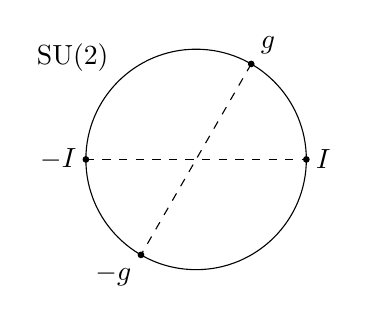
\begin{tikzpicture}[scale=0.7]
        \draw (0,0) circle (2);
        \draw[fill] (2,0) circle (0.05);
        \draw[fill] (-2,0) circle (0.05);
        \node[right] at (2,0) {$I$};
        \node[left] at (-2,0) {$-I$};
        \draw[fill] (1,1.732) circle (0.05);
        \draw[fill] (-1,-1.732) circle (0.05);
        \node[above right] at (1, 1.732) {$g$};
        \node[below left] at (-1, -1.732) {$-g$};
        \draw[dashed] (-2,0)--(2,0);
        \draw[dashed] (1, 1.732)--(-1, -1.732);
        \node[above left] at (-1.414, 1.414) {SU$(2)$};
      \end{tikzpicture}
    \end{center}

    We can in fact explicitly describe exponential map from $\mathfrak{so}(3)$ to SO$(3)$ with the following lemma. 

    \begin{lemma}[Rodrigues' Formula]
      The exponential map $exp: \mathfrak{so}(3) \longrightarrow$ SO$(3)$ is defined by 
      \begin{equation}
        e^A = \cos{\theta} I_3 + \frac{\sin{\theta}}{\theta} A + \frac{(1 - \cos{\theta})}{\theta^2} B
      \end{equation}
      where 
      \begin{equation}
        A = \begin{pmatrix}
        0&-c&b\\c&0&-a\\-b&a&0
        \end{pmatrix}, B = \begin{pmatrix}
        a^2&ab&ac\\ab&b^2&bc\\ac&bc&c^2
        \end{pmatrix}
      \end{equation}
      This formula has many applications in kinematics, robotics, and motion interpolation. 
    \end{lemma}

    \begin{theorem}
    The Lie algebras for the following classical Lie groups are summarized as follows. 
    \begin{enumerate}
      \item $\mathfrak{sl}_n \mathbb{R}$ is the real vector space of real $n \times n$ matrices with null trace.
      \item $\mathfrak{so}(n)$ is the real vector space of real $n \times n$ skew-symmetric matrices. 
      \item $\mathfrak{gl}_n \mathbb{R}$ is the real vector space of all real $n \times n$ matrices.
      \item $\mathfrak{o}(n) = \mathfrak{o}(n)$
    \end{enumerate}
    \end{theorem}
    Note that the corresponding groups $\GL(n, \mathbb{R}), \SL(n, \mathbb{R}), \mathfrak{gl}_n \mathbb{R}, \mathfrak{sl}_n \mathbb{R}$ are Lie groups, meaning that they are smooth real manifolds. We can view each of them as smooth real manifolds embedded in the $n^2$ dimensional vector space of real matrices, which is isomorphic to $\mathbb{R}^{n^2}$. 

    \begin{theorem}
      The Lie algebras $\mathfrak{gl}_ \mathbb{R}, \mathfrak{sl}_n \mathbb{R}, \mathfrak{o}(n), \mathfrak{so}(n)$ are well-defined, but only 
      \begin{equation}
        exp: \mathfrak{so}(n) \longrightarrow \text{SO}(n)
      \end{equation}
      is surjective. 
    \end{theorem}

    \begin{theorem}
      The Lie algebras for the following classical Lie groups are summarized as follows. 
      \begin{enumerate}
        \item $\mathfrak{sl}_2 \mathbb{C}$ is the real (or complex) vector space of traceless complex $n \times n$ matrices. 
        \item $\mathfrak{u}(n)$ is the real vector space of complex $n \times n$ skew-Hermitian matrices. 
        \item $\mathfrak{su}(n) = \mathfrak{u} \cap \mathfrak{sl}_2 \mathbb{C}$. It is also a real vector space. 
        \item $\mathfrak{gl}_n \mathbb{C}$ is the real (or complex) vector space of complex $n \times n$ matrices. 
      \end{enumerate}
      Note that even though the matrices in these Lie algebras have complex coefficients, we have assigned them to be in a \textbf{real} vector space, which means that we are only allowed to take real linear combinations of these elements. That is, the field we are working over is $\mathbb{R}$ (this does not contradict any of the axioms for vector spaces). For example an element $A$ in $\mathfrak{u}(n)$ or $\mathfrak{su}(n)$ must be anti-self adjoint, but $iA$ is self adjoint. 
    \end{theorem}

    Similarly, the Lie groups 
    \begin{equation}
      \GL(n, \mathbb{C}), \SL(n, \mathbb{C}), \mathfrak{gl}_n \mathbb{C}, \mathfrak{sl}_n \mathbb{C}
    \end{equation}
    are also smooth real manifolds embedded in Mat$(n, \mathbb{C}) \simeq \mathbb{C}^{n^2} \simeq \mathbb{R}^{2 n^2}$. So, we can view these four groups as manifolds embedded in $\mathbb{R}^{2 n^2}$. 

    Note some of the similarities and differences between the real and complex counterparts of these Lie groups and algebras. 
    \begin{enumerate}
      \item $\mathfrak{o}(n) = \mathfrak{so}(n)$, but $\mathfrak{u}(n) \neq \mathfrak{su}(n)$. 
      \item $exp: \mathfrak{gl}_n \mathbb{R} \longrightarrow \GL(n, \mathbb{R})$ is not surjective, but $exp: \mathfrak{gl}_n \mathbb{C} \longrightarrow \GL(n, \mathbb{C})$ is surjective due to the spectral theorem and surjectivity of $exp: \mathbb{C} \longrightarrow \mathbb{C}^*$.
      \item The exponential maps $exp: \mathfrak{u}(n) \longrightarrow \text{U}(n)$ and $exp: \mathfrak{su}(n) \longrightarrow \text{SU}(n)$ are surjective. 
      \item Still, $exp: \mathfrak{sl}_2 \mathbb{C} \longrightarrow \SL(2, \mathbb{C})$ is not surjective. This will be proved now. 
    \end{enumerate}

    \begin{theorem}
      $exp: \mathfrak{sl}_2 \mathbb{C} \longrightarrow \SL(2, \mathbb{C})$ is not surjective. 
    \end{theorem}
    \begin{proof}
      Given $M \in \SL(n, \mathbb{C})$, assume that $M = e^A$ for some matrix $A \in \mathfrak{sl}_2 \mathbb{C}$. Putting $A$ into the Jordan Normal Form $J = N A N^{-1}$ means that $J$ can either be of form
      \begin{equation}
        J = \begin{pmatrix}
        0&1\\0&0
        \end{pmatrix}, \begin{pmatrix}
        \lambda&0\\0&-\lambda
        \end{pmatrix} \implies e^J = \begin{pmatrix}
        1&1\\0&1
        \end{pmatrix}, \begin{pmatrix}
        e^\lambda&0\\0&e^{-\lambda}
        \end{pmatrix}
      \end{equation}
      which is also in JNF in $\SL(2, \mathbb{C})$. But a matrix $P \in \SL(2, \mathbb{C})$ may exist with JNF of 
      \begin{equation}
        K = \begin{pmatrix}
        -1&1\\0&-1
        \end{pmatrix}
      \end{equation}
      which is not one of the 2 forms. So, $K \not\in \im{exp} \implies exp$ is not surjective. 
    \end{proof}

    \begin{theorem}
    The exponential maps 
    \begin{align*}
      & exp: \mathfrak{u}(n) \longrightarrow \text{U}(n) \\
      & exp: \mathfrak{su}(n) \longrightarrow \text{SU}(n)
    \end{align*}
    are surjective. 
    \end{theorem}

  \subsubsection{Lie Algebra of SE(n)}

    Recall that the group of affine rigid isometries is denoted SE$(n)$. That is, 
    \begin{equation}
      \text{SE}(n) \equiv \text{SO}(n) \ltimes \text{Tran}\,\mathbb{R}^n
    \end{equation}
    We can define the matrix representation of this affine transformation as such. Given an element $g \in$ SE$(n)$ such that
    \begin{equation}
      g(x) \equiv R x + U, \; R \in \text{SO}(n), U \in \text{Tran}\, \mathbb{R}^n 
    \end{equation}
    we define the representation
    \begin{equation}
      \rho: \text{SE}(n) \longrightarrow \GL(n+1, \mathbb{R}), \rho(g) \equiv \begin{pmatrix}
      R&U\\0&1
      \end{pmatrix}
    \end{equation}
    where $R$ is a real $n\times n$ matrix in SO$(n)$ and $U$ is a real $n$-vector in Tran$\,\mathbb{R}^n \simeq \mathbb{R}^n$. We would then have
    \begin{equation}
      \rho(g) \begin{pmatrix}
      x\\1
      \end{pmatrix} \equiv \begin{pmatrix}
      R&U\\0&1
      \end{pmatrix} \begin{pmatrix}
      x\\1
      \end{pmatrix} = \begin{pmatrix}
      R x + U\\1
      \end{pmatrix} \in \mathbb{R}^{n+1}
    \end{equation}

    Clearly, SE$(n)$ is a Lie group, and the matrix representation $\varrho$ of its Lie algebra $\mathfrak{se}(n)$ can be defined as the vector space of $(n+1) \times (n+1)$ matrices of the block form 
    \begin{equation}
      A = \begin{pmatrix}
      \Omega & U \\0 & 0
      \end{pmatrix}
    \end{equation}
    where $\Omega$ is an $n \times n$ skew-symmetric matrix and $U \in \mathbb{R}^n$. Note that there are two different exponential maps here: one belonging to the abstract Lie group SE$(n)$ and another belonging to the concrete, matrix group $\GL(n+1, \mathbb{R})$. This can be represented with the commutative diagram. 
    \[\begin{tikzcd}
    \mathfrak{se}(n) \arrow{r}{exp} \arrow{d}{\varrho} & SE(n) \arrow{d} {\rho}\\
    \mathfrak{gl}_{n+1} \mathbb{R} \arrow{r}{exp} & \GL(n+1, \mathbb{R})
    \end{tikzcd}\]

    \begin{lemma}
      Given any $(n+1) \times (n+1)$ matrix of form 
      \begin{equation}
        A = \begin{pmatrix}
         \Omega & U \\0&0
        \end{pmatrix}
      \end{equation}
      where $\Omega$ is any matrix and $U \in \mathbb{R}^n$, 
      \begin{equation}
        A^k = \begin{pmatrix}
        \Omega^k & \Omega^{k-1} U \\0&0
        \end{pmatrix}
      \end{equation}
      where $\Omega^0 = I_n$, which implies that
      \begin{equation}
        e^A = \begin{pmatrix}
        e^\Omega & V U \\ 0 & 1
        \end{pmatrix}, \; V = I_n + \sum_{k \geq 1} \frac{\Omega^k}{(k+1)!}
      \end{equation}
    \end{lemma}

    \begin{theorem}
      The exponential map
      \begin{equation}
        exp: \mathfrak{se}(n) \longrightarrow SE(n)
      \end{equation}
      is well-defined and surjective. 
    \end{theorem}

\subsection{Representations of Lie Groups and Lie Algebras}

  Let $\mathcal{G}$ be an abstract group and let
  \begin{equation}
    \rho: \mathcal{G} \longrightarrow \GL(V)
  \end{equation}
  be the representation of $\mathcal{G}$. Then, let $\mathfrak{g}$ be the Lie algebra of $\mathcal{G}$, and $\mathfrak{gl}(V)$ be the Lie algebra of $\GL(V)$. Then, $\rho$ induces another homomorphism 
  \begin{equation}
    \varrho: \mathfrak{g} \longrightarrow \mathfrak{gl}(V)
  \end{equation}
  where the bracket structure (in this case, the comutator in the matrix algebra) is preserved. 
  \begin{equation}
    \varrho([X,Y]) = [\varrho(X), \varrho(Y)]
  \end{equation}
  We can visualize this induced homomorphism with the following commutative diagram, which states that $\rho \circ exp = exp \circ \varrho$. 

  \[\begin{tikzcd}
  \mathcal{G} \arrow{r}{\rho} & \GL(V)\\
  \mathfrak{g} \arrow{u}{exp} \arrow{r}{\varrho} & \mathfrak{gl}(V) \arrow{u}{exp}
  \end{tikzcd}\]

  Note that there are very crucial differences between $\rho$ and $\varrho$. First, $\rho$ is a homomorphism between \textbf{groups}, while $\varrho$ is a homomorphism between \textbf{vector spaces}. Additionally, $\GL(V)$ is a group, not a linear space, while $\mathfrak{gl}(V)$ is a linear space. Finally, note that $\GL(V)$ is restricted to only matrices with nonzero determinants, while the elements of $\mathfrak{gl}(V)$ can be any matrix. 

  \begin{example}
    The representation of SE$(n)$ to $\GL(n+1 \mathbb{R}$ and $\mathfrak{se}(n)$ to $\mathfrak{gl}_{n+1} \mathbb{R}$ induces the second homomorphism $\varrho: \mathfrak{gl}_{n+1} \mathbb{R} \longrightarrow \GL(n+1, \mathbb{R})$. 
  \end{example}

  \begin{definition}
    The direct sum of representations is a representation. That is, if $U$ is a representation and $V$ is a representation, then $U \oplus V$ is a representation. That is, if 
    \begin{equation}
      \rho_1: \mathcal{G} \longrightarrow U, \; \rho_1 (g) = \begin{pmatrix}
      u_1&u_2\\u_3&u_4
      \end{pmatrix}
    \end{equation}
    and
    \begin{equation}
      \rho_2: \mathcal{G} \longrightarrow V, \; \rho_2 (g) = \begin{pmatrix}
      v_1 & v_2 \\ v_3 & v_4
      \end{pmatrix}
    \end{equation}
    are two representations of the same group element $g \in \mathcal{G}$, then 
    \begin{equation}
      (\rho_1 \oplus \rho_2): \mathcal{G} \longrightarrow (U \oplus V), \;(\rho_1 \oplus \rho_2) (g) = \begin{pmatrix}
      u_1 & u_2 & 0 & 0 \\
      u_3 & u_4 & 0 & 0 \\
      0 & 0 & v_1 & v_2 \\
      0 & 0 & v_3 & v_4 
      \end{pmatrix}
    \end{equation}
    is a bigger representation of $g$ in $U \oplus V$. 
  \end{definition}

  \begin{definition}
    $V$ is irreducible if the only subspaces which are representations are only $V$ and $\{0\}$. 
  \end{definition}

  For our case, we will consider that any representation can be written as a direct sum of irreducible representations. We will now proceed to find an irreducible representation of $\mathfrak{sl}_2 \mathbb{C}$. This means that we want to find the smallest (lowest dimensional) vector space $V$ such that there exists a representation
  \begin{equation}
    \varrho: \mathfrak{sl}_2 \mathbb{C} \longrightarrow \mathfrak{gl}(V)
  \end{equation}
  We will write, as shorthand notation, that 
  \begin{equation}
    H = \varrho(H), X = \varrho(X), Y = \varrho(Y)
  \end{equation}
  Clearly, $H, X, Y \in \mathfrak{gl}(V) \simeq \mathfrak{gl}(\mathbb{C}^n)$. By the spectral theorem, we can find an orthonormal basis of eigenvectors $e_1, e_2, ..., e_n$ of the mapping $H$ such that
  \begin{equation}
    H e_i = \lambda_i e_i, \; \lambda_i \in \mathbb{C}
  \end{equation}
  Since $[H,X] = 2X$, it follows that
  \begin{equation}
    HX e_i - X H e_i = 2X e_i \implies H (X e_i) = (\lambda_i + 2) (X e_i)
  \end{equation}

  $\implies Xe_i$ for all $i = 1, 2, ..., n$ are also eigenvectors of $H$ with eigenvalue $(\lambda_i + 2)$, or $X e_i = 0$. So, $X$ is a "ladder operator" that maps each eigenvector $e_i$ with eigenvalue $\lambda_i$ to a different eigenvector $e_j$ with eigenvalue $\lambda_j = \lambda_i + 2$. Having nowhere to be mapped to, the eigenvector with the largest eigenvalue (which must exist since $V$ is finite dimensional) will get mapped to the $0$ vector by $X$. Let us denote this eigenvector having the maximum eigenvalue $m$, as $v_m$. 

  Similarly, $[H,Y] = -2Y$ implies that
  \begin{equation}
    HY e_i - YH e_i = -2Y e_i \implies H(Y e_i) = (\lambda_i - 2)(Y e_i)
  \end{equation}

  implying that $Y$ maps each eigenvector $e_i$ with eigenvaue $\lambda_i$ to another eigenvector $e_j$ with eigenvalue $\lambda_j = \lambda_i - 2$, except for the eigenvector with smallest eigenvalue, which gets mapped to $0$. Since $Y$ clearly maps each eigenvector to a different eigenvector that has a strictly decreasing eigenvalue, we can construct a basis of $V$ to be
  \begin{equation}
    \{v_m, Y v_m, Y^2 v_m, Y^3 v_m, ..., Y^{n-1} v_m\}
  \end{equation}
  (remember that $Y^n v_m = 0$). So, elements of $\mathfrak{sl}_2 \mathbb{C}$ acts on the space $V$ with basis above. To continue, we introduce the following proposition. 

  \begin{proposition}
    \begin{equation}
      X Y^j v_m = j(m-j+1) Y^{j-1} v_m
    \end{equation}
  \end{proposition}
  \begin{proof}
    By induction on $j$ using bracket relations.
  \end{proof}

  $V$ is $n$-dimensional. Since $Y^n v_m = 0$ and $Y^{n-1} v_m \neq 0$, we use the proposition above to get
  \begin{equation}
    0 = X Y^n v_m = n (m-n+1) Y^{n-1} v_m \implies m-n+1=0
  \end{equation}
  So, $n = m+1$, which means that the eigenvalues of $H$ are
  \begin{equation}
    m, m-2, m-4, \ldots, m - 2(n-1) = -m
  \end{equation}

  and we are done. We now classify the 1, 2, and 3 dimensional irreducible representations of $\mathfrak{sl}_2 \mathbb{C}$. 
  \begin{enumerate}
    \item When $n = 1$ (i.e. dimension is 1), $m = n-1 = 0$, meaning that the greatest (and only) eigenvalue is $0$. That is, 
      \begin{equation}
        H v_0 = 0,\; X v_0 = 0,\; Y v_0 = 0
      \end{equation}
    which is the trivial representation of $\mathfrak{sl}_2 \mathbb{C}$. Explicitly, we can completely define the representation (which is a linear homomorphism) with the three equations. 
    \begin{equation}
      \varrho(H) = (0),\; \varrho(X) = (0),\; \varrho(Y) = (0)
    \end{equation}

    \item When $n = 2$ and $m=1$. We now look for a 2 dimensional irreducible representation. The eigenvalues are $1$ and $-1$, with $\{v_1, v_{-1}\}$ as a basis of 2 dimensional space $V$. Then we have 
      \begin{align*}
        & Hv_1 = v_1, \; Hv_{-1} = - v_{-1} \\
        & X v_1 = 0, \; X v_{-1} = v_1 \\
        & Y v_1 = v_{-1}, \; Y v_{-1} = 0
      \end{align*}
    which explicitly translates to the representation $\varrho$ being defined
    \begin{equation}
      \varrho(H) = \begin{pmatrix}
      1&0\\0&-1
      \end{pmatrix}, \; \begin{pmatrix}
      0&1\\0&0
      \end{pmatrix}, \; \begin{pmatrix}
      0&0\\1&0
      \end{pmatrix}
    \end{equation}

    \item When $n=3 \implies m=2$, the basis is $\{v_{-2}, v_0, v_2\}$ with eigenvalues $2, 0, -2$, and the irreducible representation $\varrho$ is defined
      \begin{equation}
        \varrho(H) = \begin{pmatrix}
        2&&\\&0&\\&&-2
        \end{pmatrix}, \varrho(Y) = \begin{pmatrix}
        0&0&0\\1&0&0\\0&1&0
        \end{pmatrix}, \varrho(X) = \begin{pmatrix}
        0&1&0\\0&0&1\\0&0&0
        \end{pmatrix}
      \end{equation}

    \item The same process continues on for $n=4, 5, ...$, and this entirely classifies the irreducible representations of $\mathfrak{sl}_2 \mathbb{C}$. 
  \end{enumerate}

  \subsubsection{Tensor Products of Group Representations}

    \begin{definition}
      If $V$ and $W$ are two different representations of a group $\mathcal{G}$, then we know that $V \oplus W$ is also a representation of $\mathcal{G}$. Furthermore, the tensor product space $V \otimes W$ also defines a representation of $\mathcal{G}$. That is, given representations
      \begin{align*}
        & \rho_V: \mathcal{G} \longrightarrow \GL(V) \\
        & \rho_W: \mathcal{G} \longrightarrow \GL(W)
      \end{align*}
      The homomorphism 
      \begin{equation}
        \rho_V \otimes \rho_W: \mathcal{G} \longrightarrow \GL(V \otimes W)
      \end{equation}
      is also a representation of $\mathcal{G}$, which is defined
      \begin{equation}
        (\rho_V \otimes \rho_W)(g) (v \otimes w) \equiv \rho_V (g) (v) \otimes \rho_W (g) (w)
      \end{equation}
      or represented in shorthand notation, 
      \begin{equation}
        g(v \otimes w) \equiv (g v) \otimes (g w)
      \end{equation}
      We know that exp$(H)$ acts on $V$ and $W$ since it is an element of $\GL(V)$ and $\GL(W)$. This means that
      \begin{equation}
        exp(H)(v \otimes w) \equiv \big( exp(H)(v)\big) \otimes \big( exp(H)(w)\big)
      \end{equation}
      If $H$ ($= \rho_V (H)$ or $\rho_W(H)$) has an eigenvalue $\lambda$ on $v$ in $V$ and eigenvalue $\mu$ on $w$ in $W$, then 
      \begin{equation}
        exp(H) (v \otimes w) = (e^\lambda v) \otimes (e^\mu w) = e^{\lambda + \mu} v \otimes w
      \end{equation}
      That is, eigenvalues of $H$ \textbf{add} on tensor products. 
    \end{definition}

    \begin{example}
      Recall that the $2$ dimensional representation $V$ of $\mathfrak{sl}_2 \mathbb{C}$ has eigenvalues $1$ and $-1$ (with corresponding eigenvectors $e_1$ and $e_{-1}$). So, $V \otimes V$ has eigenvalues 
      \begin{align*}
        & (-1) + (-1) = -2, \;\; (-1) + 1 = 0 \\
        & 1 + (-1) = 0, \;\; 1 + 1 = 2
      \end{align*}
      Therefore, the eigenvalues of $V \otimes V$ is $-2$ (geometric multiplicity of 1), $0$ (geometric multiplicity of 2), and $2$ (geometric multiplicity of 1), (Notation-wise, the $n$-dimensional irreducible representation of $\mathfrak{sl}_2 \mathbb{C}$ is denoted $\mathbf{n}$.) which means that
      \begin{equation}
        \mathbf{2} \otimes \mathbf{2} = \mathbf{3} \oplus \mathbf{1}
      \end{equation}
      We can decompose $V \otimes V$ into its symmetric and exterior power components. Sym$^2 V$ has basis (of eigenvectors)
      \begin{equation}
        \{e_{-1} \odot e_{-1}, \; e_{-1} \odot e_1, \; e_1 \odot e_1\}
      \end{equation}
      where the corresponding eigenvalues are $-2$, $0$, and $2$, respectively. So, $\dim{Sym^2 V} = 3$, which means that $Sym^2 V = \mathbf{3}$. As for the exterior power component of $V$, $\Lambda^2 V$ has basis 
      \begin{equation}
        \{e_{-1} \wedge e_1\}
      \end{equation}
      with eigenvalue $= 0 \implies \dim{\Lambda^2 V} = 1$, meaning that $\Lambda^2 V = \mathbf{1}$. Therefore, 
      \begin{equation}
        V \otimes V = Sym^2 V \oplus \Lambda^2 V = \mathbf{3} \oplus \mathbf{1}
      \end{equation}
    \end{example}

\subsection{Topological Decompositions of Lie Groups}

  \begin{definition}
    Let us define 
    \begin{enumerate}
      \item S$(n)$ is the vector space of real, symmetric $n \times n$ matrices. 
      \item SP$(n)$ is the set of symmetric, positive semidefinite matrices. 
      \item SPD$(n)$ is the set of symmetric, positive definite matrices. 
    \end{enumerate}
    Note that SP$(n)$ and SPD$(n)$ are not even vector spaces at all. 
  \end{definition}

  \begin{lemma}
    The exponential map 
    \begin{equation}
      exp: S(n) \longrightarrow SPD(n)
    \end{equation}
    is a homeomorphism. One may be tempted to call S$(n)$ the Lie algebra of SPD$(n)$, but this is not the case. S$(n)$ is not even a Lie algebra since the commutator is not algebraically closed. Furthermore, SPD$(n)$ is not even a multiplicative group (since matrix multiplication is not closed). 
  \end{lemma}

  Recall from linear algebra the Polar Decomposition. We express this result in a slightly modified way. 

  \begin{theorem}[Polar Decomposition]
    Given a Euclidean space $\mathbb{E}^n$ and any linear endomorphism $f$ of $\mathbb{E}^n$, there are two positive definite self-adjoint linear maps $h_1, h_2 \in$ End$(\mathbb{E}^n)$ and $g \in$ O$(n)$ such that
    \begin{equation}
      f = g \circ h_1 = h_2 \circ g
    \end{equation}
    That is, such that $f$ can be decomposed into the following compositions of functions that commute. 

    \[\begin{tikzcd}
    \mathbb{E}^n \arrow{r}{h_2} & \mathbb{E}^n \\
    \mathbb{E}^n \arrow{u}{g} \arrow{ur}{f} \arrow{r}{h_1} & \mathbb{E}^n \arrow{u}{g}
    \end{tikzcd}\]

    This means that there is a bijection between $Mat(n, \mathbb{R})$ and $O(n) \times SP(n)$. If $f$ is an automorphism, then this decomposition is unique. 
  \end{theorem}

  \begin{corollary}
    The two topological groups are homeomorphic. 
    \begin{equation}
      GL(n, \mathbb{R}) \cong O(n) \times SPD(n)
    \end{equation}
  \end{corollary}

  \begin{corollary}
    For every invertible real matrix $A \in GL(n, \mathbb{R})$, there exists a unique orthogonal matrix $R$ and unique symmetric matrix $S$ such that
    \begin{equation}
      A = R e^S
    \end{equation}
    $\implies$ there is a bijection between $\GL(n, \mathbb{R})$ and $O(n) \times S(n) \simeq \mathbb{R}^{n(n+1)/2}$. Moreover, they are homeomorphic. That is, 
    \begin{equation}
      \GL(n, \mathbb{R}) \simeq O(n) \times S(n) \simeq O(n) \times \mathbb{R}^{n(n+1)/2}
    \end{equation}
    This essentially reduces the study of $\GL(n, \mathbb{R})$ to the study of $O(n)$, which is nice since $O(n)$ is compact. 
  \end{corollary}

  \begin{corollary}
    Given a real matrix $A$, if $\det{A} > 0$, then we can decompose $A$ as
    \begin{equation}
      A = R e^S
    \end{equation}
    where $R \in SO(n)$ and $S \in S(n)$. 
  \end{corollary}

  \begin{corollary}
    There exists a bijection between
    \begin{equation}
      \SL(n, \mathbb{R}) \text{ and } SO(n) \times (S(n) \cap \mathfrak{sl}_n \mathbb{R})
    \end{equation}
  \end{corollary}
  \begin{proof}
    $A \in \SL(n, \mathbb{R}) \implies 1 = \det{A} = \det{R} \det{e^S} = \det{e^S} \implies \det{e^S} = e^{\Tr{S}} = 1 \implies \Tr{S} = 0 \implies S \in$ S$(n) \cap \mathfrak{sl}_n \mathbb{R}$. 
  \end{proof}

  \begin{definition}
    Let us define
    \begin{enumerate}
      \item H$(n)$ is the real vector space of $n \times n$ Hermitian matrices. 
      \item HP$(n)$ is the set of Hermitian, positive semidefinite $n \times n$ matrices. 
      \item HPD$(n)$ is the set of Hermitian, positive definite $n \times n$ matrices. 
    \end{enumerate}
    Similarly, HP$(n)$ and HPD$(n)$ are not vector space. They are just sets. 
  \end{definition}

  \begin{lemma}
    The exponential mapping
    \begin{equation}
      exp: H(n) \longrightarrow HPD(n)
    \end{equation}
    is a homeomorphism. 
  \end{lemma}

  However again, HPD$(n)$ is not a Lie group (multiplication is not algebraically closed) nor is H$(n)$ a Lie algebra (commutator is not algebraically closed). By the polar form theorem of complex $n \times n$ matrices, we have a (not necessarily unique) bijection between
  \begin{equation}
    \text{Mat}(n, \mathbb{C}) \text{ and } U(n) \times HP(n)
  \end{equation}
  which implies that
  \begin{equation}
    \GL(n, \mathbb{C}) \cong U(n) \times HPD (n)
  \end{equation}

  \begin{corollary}
    For every complex invertible matrix $A$, there exists a unique decomposition
    \begin{equation}
      A = U e^S
    \end{equation}
    where $U \in U(n)$ and $S \in H(n)$, which implies that the following groups are homeomorphic. 
    \begin{align*}
      \GL(n, \mathbb{C}) & \cong U(n) \times H(n) \\
      & \cong U(n) \times \mathbb{R}^{n^2}
    \end{align*} 
    This essentially reduces the study of $\GL(n, \mathbb{C})$ to that of U$(n)$. 
  \end{corollary}

  \begin{corollary}
    There exists a bijection between 
    \begin{equation}
      \SL(n, \mathbb{C}) \text{ and } SU(n) \times (H(n) \cap \mathfrak{sl}_n \mathbb{C})
    \end{equation}
  \end{corollary}
  \begin{proof}
    Similarly, when $A = U e^S$, we know that $|\det{U}| = 1$ and $\Tr{S}$ is real (since by the Spectral theorem, every self adjoint matrix has a real spectral decomposition). Since $S$ is Hermitian, this implies that $\det{e^S} > 0$. If $A \in \SL(n, \mathbb{C})$, then $\det{A} = 1 \implies \det{e^S} = 1 \implies S \in H(n) \cap \mathfrak{sl}_n \mathbb{C}$. 
  \end{proof}

\subsection{Linear Lie Groups}

  We will assume that the reader has the necessary background knowledge in manifolds, chart mappings, diffeomorphisms, tangent spaces, and transition mappings. 

  Recall that the algebra of real $n \times n$ matrices Mat$(n, \mathbb{R})$ is bijective to $\mathbb{R}^{n^2}$, which is a topological space. Therefore, this bijection 
  \begin{equation}
    i:(\mathbb{R}^{n^2}, \tau_E) \longrightarrow \text{Mat}(n, \mathbb{R})
  \end{equation}
  induces a topology on Mat$(n, \mathbb{R})$, defined 
  \begin{equation}
    \tau_M \equiv \{U \in \text{Mat}(n, \mathbb{R}) \; | \; e^{-1} (U) \in \tau_E\}
  \end{equation}
  With this, consider the subset
  \begin{equation}
    \GL(n, \mathbb{R}) \subset \text{Mat}(n, \mathbb{R})
  \end{equation}
  where
  \begin{equation}
    \GL(n, \mathbb{R}) \equiv \{x \in \text{Mat}(n, \mathbb{R}) \;|\; \det{x} \neq 0\}
  \end{equation}
  This set, as we expect, is a multiplicative group. 

  \begin{definition}
    The \textbf{general linear group}, denoted $\GL(n, \mathbb{R})$ is the set of $n \times n$ matrices with nonzero determinant. The more technical definition is that $\GL(n, \mathbb{R})$ is really just the automorphism group of $\mathbb{R}^n$, 
    \begin{equation}
      \GL(n, \mathbb{R}) \equiv \text{Aut}(\mathbb{R}^n)
    \end{equation}
    but it is customary to assume a basis on $\mathbb{R}^n$ in order to realize $\GL(n, \mathbb{R})$ as a matrix group. Note that the procedure of assuming a basis on $\mathbb{R}^n$ is the same as defining a representation of the abstract group $\GL(n, \mathbb{R})$. Both assigns a real $n \times n$ matrix to each element of $\GL(n, \mathbb{R})$. 
  \end{definition}

  In this way, we can view $\GL(n, \mathbb{R})$ as a topological space in $\mathbb{R}^{n^2}$, and it is fine to interpret $\GL(n, \mathbb{R})$ as a matrix group rather than an abstract group. 

  Since the matrix representation of $\GL(n, \mathbb{R})$ is always well defined, the abstract subgroups of $\GL(n, \mathbb{R})$, which are $\SL(n, \mathbb{R}), O(n)$, and $SO(n)$, also have well defined matrix representations (that we are all familiar with). Additionally, since there exists a bijection
  \begin{equation}
    \text{Mat}(n, \mathbb{C}) \cong \mathbb{C}^{n^2} \cong \mathbb{R}^{2 n^2}
  \end{equation}
  we can view $\GL(n, \mathbb{C})$ as a subset of $\mathbb{R}^{2n^2}$, meaning that the subgroups $\SL(n, \mathbb{C}), U(n)$, and $SU(n)$ of $\GL(n, \mathbb{C})$ can also be viewed as subsets of $\mathbb{R}^{2n^2}$. This also applies to $SE(n)$ since it is a subgroup of $\SL(n+1, \mathbb{R})$. We formally state it now. 

  \begin{proposition}
    SE$(n)$ is a linear Lie group. 
  \end{proposition}
  \begin{proof}
    The matrix representation of elements $g \in SE(n)$ is 
    \begin{equation}
      \rho(g) \equiv \begin{pmatrix}
      R_g & U_g \\ 0 & 1
      \end{pmatrix}, \; R_g \in SO(n), U_g \in \mathbb{R}^n
    \end{equation}
    But such matrices also belong to the bigger group $\SL(n+1, \mathbb{R}) \implies SE(n) \subset \SL(n+1, \mathbb{R})$. Moreover, this canonical embedding 
    \begin{equation}
      i: SE(n) \longrightarrow \SL(n+1, \mathbb{R})
    \end{equation}
    is a group homomorphism since
    \begin{align*}
      i\big( \rho(g_1 \cdot g_2) \big) & = \begin{pmatrix}
      RS & RV + U \\ 0 & 1
      \end{pmatrix} \\
      & = \begin{pmatrix}
      R & U \\ 0 & 1
      \end{pmatrix} \begin{pmatrix}
      S & V \\ 0 & 1
      \end{pmatrix} = \rho \big( i(g_1) \cdot i(g_2) \big) 
    \end{align*}
    and the inverse is given by 
    \begin{equation}
      \begin{pmatrix}
      R & U \\ 0 & 1
      \end{pmatrix}^{-1} = \begin{pmatrix}
      R^{-1} & - R^{-1} U \\ 0 & 1
      \end{pmatrix} = \begin{pmatrix}
      R^T & - R^T U \\ 0 & 1
      \end{pmatrix}
    \end{equation}
    is also consistent between the inverse operation in SE$(n)$ and $\SL(n+1, \mathbb{R})$. Therefore, SE$(n)$ is a subgroup of $\SL(n+1, \mathbb{R})$, which is a subgroup of $\GL(n+1, \mathbb{R})$. 
  \end{proof}

  Note that even though SE$(n)$ is diffeomorphic (a topological relation) to SO$(n) \times \mathbb{R}^n$, it is \textbf{not} isomorphic (an algebraic relation) sicne group operations are not preserved. Therefore, we write this "equality" as a semidirect product of groups. 
  \begin{equation}
    SE(n) \equiv SO(n) \ltimes \mathbb{R}^n
  \end{equation}

  Therefore, all of the classical Lie groups that we have mentioned can be viewed as subsets of $\mathbb{R}^N$ (with the subspace topology) and as subgroups of $\GL(N, \mathbb{R})$ for some big enough $N$. This defines a special family of Lie groups, called linear Lie groups. 

  \begin{definition}
    A \textbf{linear Lie group} is a subgroup of $\GL(n, \mathbb{R})$ for some $n \geq 1$ which is also a smooth manifold in $\mathbb{R}^{n^2}$. 
  \end{definition}

  \begin{theorem}[Von Neumann, Cartan]
    A closed subgroup $\mathcal{G}$ of $\GL(n, \mathbb{R})$ is a linear Lie group. That is, a closed subgroup $\mathcal{G}$ of $\GL(n, \mathbb{R})$ is a smooth manifold in $\mathbb{R}^{n^2}$.
  \end{theorem}

  \begin{definition}
    Since a linear Lie group $\mathcal{G}$ is a smooth submanifold in $\mathbb{R}^N$, we can take its tangent space at the identity element $I$, which is defined 
    \begin{equation}
      T_I \mathcal{G} \equiv \{p^\prime (0) \;|\; p: I \subset \mathbb{R} \longrightarrow \mathcal{G}, p(0) = I\}
    \end{equation}
    where $p$ is a path function on $\mathcal{G}$. 
  \end{definition}

  Note that we haven't mentioned anything about the exponential map up to now. We mention the relationship between this map and the Lie algebra with the following theorem. 

  \begin{theorem}
    Let $\mathcal{G}$ be a linear Lie group. The set $\mathfrak{g}$ defined such that
    \begin{equation}
      \mathfrak{g} \equiv \{X \in \text{Mat}(n, \mathbb{R}) \; | \; e^{t X} \in \mathcal{G} \; \forall t \in \mathbb{R}\}
    \end{equation}
    is equal to the tangent space of $\mathcal{G}$ at the identity element. That is, 
    \begin{equation}
      \mathfrak{g} = T_I \mathcal{G}
    \end{equation}
    Furthermore, $\mathfrak{g}$ is closed under the commutator 
    \begin{equation}
      [A,B] \equiv A B - B A
    \end{equation}
  \end{theorem}

  This theorem ensures that given a linear Lie group $\mathcal{G}$, the tangent space $\mathfrak{g}$ exists and is closed under the commutator. We formally define this space. 

  \begin{definition}
    The Lie algebra of a linear Lie group is a real vector space (of matrices) together with a algebraically closed bilinear map 
    \begin{equation}
      [A,B] \equiv A B - B A
    \end{equation}
    called the \textbf{commutator}. 
  \end{definition} 

  The definition of $\mathfrak{g}$ given in the previous theorem shows that 
  \begin{equation}
    exp: \mathfrak{g} \longrightarrow \mathcal{G}
  \end{equation}
  is well defined. In general, exp is neither injective nor surjective. Visually, this exponential mapping is what connects the Lie algebra, i.e. the tangent space of manifold $\mathcal{G}$ to the actual Lie group $\mathcal{G}$. To define the inverse map that maps Lie group elements to Lie algebra ones, we can simply just compute the tangent vectors of the manifold $\mathcal{G}$ at the identity $I$ by taking the derivative of arbitrary path functions in $\mathcal{G}$. That is, for every $X \in T_I \mathcal{G}$, we define the smooth curve 
  \begin{equation}
    \gamma_X: t \mapsto e^{tX}
  \end{equation}
  where $\gamma_X(0) = I$. If we take the derivative of this curve, with respect to $t$ at $t = 0$, we will get the tangent vector $X$ corresponding to that group element $g = e^{X}$. More visually, we just need to take the collection of all smooth path functions $\gamma$ on manifold $\mathcal{G}$ such that $\gamma(0) = I$. Then, taking the derivative of all these paths at $t = 0$ will produce the collection of all tangent vectors at the identity element. We show this process in the following examples. 

  \begin{theorem}
    The matrix representation of $\mathfrak{sl}_n \mathbb{R}$ is precisely the set of traceless $n \times n$ matrices. 
  \end{theorem}

  \begin{proof}
    Clearly, $\mathfrak{sl}_n \mathbb{R}$ is a vector space since it is a Lie algebra. So, $X \in \mathfrak{sl}_n \mathbb{R} \implies t X \in \mathfrak{sl}_n \mathbb{R}$ for all $t \in \mathbb{R} \implies \det{e^{tX}} = 1$ for all $t \in \mathbb{R}$, for all $X \in \mathfrak{sl}_n \mathbb{R}$. But we use the identity 
    \begin{align*}
      \det{e^{tX}} = e^{\Tr{(tX)}} & \implies 1 = e^{\Tr{(t X)}} \\
      & \implies \Tr{(tX)} = 0 \\
      & \implies \Tr{(X)} t = 0 \implies \Tr{X} = 0
    \end{align*}
  \end{proof}
  We now provide an alternative, better proof. We first need a lemma. 

  \begin{lemma}
    $\det^\prime (I) = \Tr$. That is, the differential of the $\det$ operator, evaluated at the identity matrix, is equal to the trace. That is, given any matrix $T$ in the vector space of matrices, 
  \end{lemma}
  \begin{proof}
    \begin{align*}
      \det^\prime (I) (T) = \nabla_T \det(I) \\
      & = \lim_{\varepsilon \rightarrow 0} \frac{\det{(I + \varepsilon T)} - \det{I}}{\varepsilon} \\
      & = \lim_{\varepsilon \rightarrow 0} \frac{\det{(I + \varepsilon T)} - 1}{\varepsilon}
    \end{align*}
    Clearly, $\det(I + \varepsilon(T)) \in \mathbb{R}[\varepsilon]$, where the constant term of the polynomial approaches $1$ and the linear term (coefficient of $\varepsilon$) is $\Tr{T}$. So, 
    \begin{equation}
      \nabla_T \det{I} = \lim_{\varepsilon \rightarrow 0} ... + \Tr{T} = \Tr{T}
    \end{equation}
  \end{proof}

  This means that the instantaneous rate at which $\det$ changes at $I$ when traveling in direction $T$ is directly proportional to $\Tr{T}$. Now, we provide an alternative proof of the theorem. 
  \begin{proof}
    Let $R: \mathbb{R} \longrightarrow \SL(n, \mathbb{R})$ such that $R(0) = I$. Then, by definition, $\im{R} \subset \SL(n, \mathbb{R}) \implies \det{(R(t))} = 1$ for all $t \in (-\varepsilon, \varepsilon)$. Compute the derivative of the mapping $\det \circ R$. 
    \begin{align*}
        (\det \circ  R) (t) = 1 & \implies \det^\prime \big( R(t) \big) \cdot R^\prime (t) \\ 
        & \implies \det^\prime (I) = \det^\prime \big(R(t)\big) = 0 
    \end{align*}
    We now use the previous lemma get that 
    \begin{equation}
      \det^\prime \big( R^\prime(0)\big) = \det^\prime (I)=0 \implies \Tr{R^\prime(0)} = 0
    \end{equation}
  \end{proof} 

  \begin{theorem}
    The matrix representation of $\mathfrak{so}(n)$ is precisely the set of antisymmetric matrices. 
  \end{theorem}
  \begin{proof}
    Let $R: \mathbb{R} \longrightarrow SO(n)$ be a arbitrary smooth curve in $\SL(n)$ such that $R(0) = I$. Then, for all $t \in (-\epsilon, \epsilon)$, 
    \begin{equation}
      R(t) R(t)^T = I
    \end{equation}
    Taking the derivative at $t = 0$, we get
    \begin{equation}
      R^\prime (0) R(0)^T + R(0) R^\prime(0)^T = 0 \implies R^\prime (0) + R^\prime(0)^T = 0
    \end{equation}
    which states that the tangent vector $X = R^\prime (0)$ is skew symmetric. Since the diagonal elements of a skew symmetric matrix are $0$, the trace is $0$ and the condition that $\det{R} = 1$ yields nothing new. This shows that $\mathfrak{o}(n) = \mathfrak{so}(n)$. 
  \end{proof}




  We have only worked with linear Lie groups so far. The reason that linear Lie groups are so nice to work with is because they have well defined matrix representations. This allows us to have concrete structures on these groups and their Lie algebras. 
  \begin{enumerate}
    \item A linear Lie group is concretely defined as a submanifold of $\mathbb{R}^N$, while a general one is an abstract manifold. 
    \item The Lie bracket with regards to a linear Lie group is defined to be the commutator 
      \begin{equation}
        [A,B] \equiv A B - B A
      \end{equation}
    but for elements that are not matrices this doesn't make sense. 

    \item The exponential map from the algebra to the group is defined
      \begin{equation}
        e^A \equiv \sum_{k=0}^\infty \frac{1}{k!} A^k
      \end{equation}
    but if $A$ is not a matrix, then exp cannot be defined this way.
  \end{enumerate}
  We seek to generalize these concepts to abstract Lie groups, but we will do this in the next section. 

  \subsubsection{Lie Algebras of SO(3) and SU(2), Revisited}

    \begin{example}
      The Lie algebra $\mathfrak{so}(3)$ is the real vector space of $3 \times 3$ skew symmetric matrices of form 
      \begin{equation}
        \begin{pmatrix}
        0 & -d & c \\ d & 0 & -b \\ -c & b & 0
        \end{pmatrix}
      \end{equation}
      where $b, c, d \in \mathbb{R}$. The Lie bracket $[A,B]$ of $\mathfrak{so}(3)$ is also just the usual commutator. 

      We can define an isomorphism of Lie algebras $\psi: (\mathbb{R}^3, \times) \longrightarrow \mathfrak{so}(3)$ (where $\times$ is the cross product) by the formula 
      \begin{equation}
        \psi(b, c, d) \equiv \begin{pmatrix}
        0 & -d & c \\
        d & 0 & -b \\
        -c & b & 0
        \end{pmatrix}
      \end{equation}
      where, by definition, 
      \begin{equation}
        \psi(u \times v) = [\psi(u), \psi(v)]
      \end{equation}
      It is also easily verified that for all $u, v \in \mathbb{R}^3$, 
      \begin{equation}
        \psi(u) (v) = u \times v
      \end{equation}
    \end{example}

    \begin{example}
      Similarly, we can see that $\mathfrak{su}(2)$ is the real vector space consisting of all complex $2 \times 2$ skew Hermitian matrices of null trace, which is of form
      \begin{equation}
        i(d \sigma_1 + c \sigma_2 + b \sigma_3) = \begin{pmatrix}
        i b & c + i d\\
        -c + i d & - i b
        \end{pmatrix}
      \end{equation}
      where $\sigma_1, \sigma_2, \sigma_3$ are the Pauli spin matrices. We can also define an isomorphism of Lie algebras $\varphi: (\mathbb{R}^3, \times) \longrightarrow \mathfrak{su}(2)$ by the formula
      \begin{equation}
        \varphi(b, c, d) = \frac{i}{2} (d \sigma_1 + c \sigma_2 + b \sigma_3) = \frac{1}{2} \begin{pmatrix}
        i b & c + i d\\
        -c + i d & - i b
        \end{pmatrix}
      \end{equation}
      where, by definition of ismorphism, we have
      \begin{equation}
        \varphi(u \times v) = [\varphi(u), \varphi(v)]
      \end{equation}
    \end{example}

    We now restate the connection between the groups SO$(3)$ and SU$(2)$. Note that letting $\theta = \sqrt{b^2 + c^2 + d^2}$, we can write 
    \begin{equation}
      A = \frac{1}{\theta} (d \sigma_1 + c \sigma_2 + b \sigma_3) = \frac{1}{\theta} \begin{pmatrix}
      i b & c + i d\\
      -c + i d & - i b
      \end{pmatrix}
    \end{equation}
    such that $A^2 = I$. With this, we can rewrite the exponential map as 
    \begin{equation}
      exp: \mathfrak{su}(2) \longrightarrow SU(2), \; exp(i \theta A) = \cos{\theta} I  + i \sin{\theta} A
    \end{equation}
    As for the isomorphism $\varphi: (\mathbb{R}^3, \times) \longrightarrow \mathfrak{su}(2)$, we have
    \begin{equation}
      \varphi(b, c, d) \equiv \frac{1}{2} \begin{pmatrix}
      i b & c + i d\\
      -c + i d & - i b
      \end{pmatrix} = i \frac{\theta}{2} A
    \end{equation}
    Similarly, we can view the exponential map $exp: (\mathbb{R}^3, \times) \longrightarrow SU(2)$ as 
    \begin{equation}
      exp(\theta v) = 
    \end{equation}


    \begin{example}
      The lie algebra $\mathfrak{se}(n)$ is the set of all matrices of form 
      \begin{equation}
        \begin{pmatrix}
        B & U \\ 0 & 0
        \end{pmatrix}
      \end{equation}
      where $B \in \mathfrak{so}(n)$ and $U \in \mathbb{R}^n$. The Lie bracket is given by
      \begin{equation}
        \begin{pmatrix}
        B & U \\ 0 & 0
        \end{pmatrix} \begin{pmatrix}
        C & V \\ 0 & 0
        \end{pmatrix} - \begin{pmatrix}
        C & V \\ 0 & 0
        \end{pmatrix} \begin{pmatrix}
        B & U \\ 0 & 0
        \end{pmatrix} = \begin{pmatrix}
        BC - CB & BV - CU \\ 0 & 0
        \end{pmatrix}
      \end{equation}
    \end{example}

\subsection{Abstract Lie Groups}

  \begin{definition}
    A (real) \textbf{Lie group} $\mathcal{G}$ is a group $\mathcal{G}$ that is also a real, finite-dimensional smooth manifold where  group multiplication and inversion are smooth maps. 
  \end{definition}

  \begin{definition}
    A (real) Lie algebra $\mathfrak{g}$ is a real vector space with a map 
    \begin{equation}
      [\cdot, \cdot]: \mathfrak{g} \times \mathfrak{g} \longrightarrow \mathfrak{g}
    \end{equation}
    called the Lie bracket satisfying bilinearity, antisymmetricity, and the Jacobi Identity. 
  \end{definition}

  To every Lie group $\mathcal{G}$ we can associate a Lie algebra $\mathfrak{g}$ whose underlying vector space is the tangent space of $\mathcal{G}$ at the identity element. Additionally, the exponential map allows us to map elements from the Lie algebra to the Lie group. These concrete definitions in the context of linear Lie groups is easy to work with, but has some minor problems: to use it we first need to represent a Lie group as a group of matrices, but not all Lie groups can be represented in this way. 

  To do this, we must introduce further definitions. 

  \begin{definition}
    Let $M_1$ ($m_1$-dimensional) and $M_2$ ($m_2$ dimensional) be manifolds in $\mathbb{R}^N$. For any smooth function $f: M_1 \longrightarrow M_2$ and any $p \in M_1$, the function 
    \begin{equation}
      f^\prime_p: T_p M_1 \longrightarrow T_{f(p)} M_2
    \end{equation}
    called the \textbf{tangent map, derivative, or differential} of $f$ at $p$, is defined as follows. For every $v \in T_p M_1$ and every smooth curve $\gamma: I \longrightarrow M_1$ such that $\gamma(0) = p$ and $\gamma^\prime (0) = v$ , 
    \begin{equation}
      f^\prime_p(v) \equiv (f \circ \gamma)^\prime (0)
    \end{equation}
    The map $f^\prime_p$ is also denoted $d f_p$ and is a linear map. 
  \end{definition}

  \begin{definition}
    Given two Lie groups $\mathcal{G}_1$ and $\mathcal{G}_2$, a \textbf{homomorphism of Lie groups} is a function 
    \begin{equation}
      f: \mathcal{G}_1 \longrightarrow \mathcal{G}_2
    \end{equation}
    that is both a group homomorphism and a smooth map (between manifolds $\mathcal{G}_1$ and $\mathcal{G}_2$). An \textbf{isomorphism of Lie groups} is a bijective function $f$ such that both $f$ and $f^{-1}$ are homomorphisms of Lie groups. 
  \end{definition}

  \begin{definition}
    Given two Lie algebras $\mathfrak{g}_1$ and $\mathfrak{g}_2$, a \textbf{homomorphism of Lie algebras} is a function 
    \begin{equation}
      f: \mathfrak{g}_1 \longrightarrow \mathfrak{g}_2
    \end{equation}
    that is a linear homomorphism that preserves Lie brackets; that is, 
    \begin{equation}
      f([A,B]) = [f(A), f(B)]
    \end{equation}
    for all $A, B \in \mathfrak{g}$. An \textbf{isomorphism of Lie algebras} is a bijective function $f$such that both $f$ and $f^{-1}$ are homomorphisms of Lie algebras. 
  \end{definition}

  \begin{proposition}
    If $f: \mathcal{G}_1 \longrightarrow \mathcal{G}_2$ is a homomorphism of Lie groups, then 
    \begin{equation}
      f_I^\prime: \mathfrak{g}_1 \longrightarrow \mathfrak{g}_2
    \end{equation}
    is a homomorphism of Lie algebras. 
  \end{proposition}

  We have explained how to construct the Lie bracket (as the commutator) of the Lie algebra of a linear Lie group, but we have not defined how to construct the Lie bracket for general Lie groups. There are several ways to do this, and we describe one such way through \textbf{adjoint representations}. 

  \begin{definition}
    Given a Lie group $\mathcal{G}$, we define a \textbf{left translation} as the map
    \begin{equation}
      L_a: \mathcal{G} \longrightarrow \mathcal{G}, \; L_a (b) \equiv a b
    \end{equation}
    for all $b \in \mathcal{G}$. Similarly, the \textbf{right translation} is defined
    \begin{equation}
      R_a: \mathcal{G} \longrightarrow \mathcal{G}, \; R_a (b) \equiv b a
    \end{equation}
    for all $b \in \mathcal{G}$. 
  \end{definition}

  Both $L_a$ and $R_a$ are diffeomorphisms. Additionally, given the automorphism
  \begin{equation}
    R_{a^{-1}} L_a \equiv R_{a^{-1}} \circ L_a, \; R_{a^{-1}} L_a (b) \equiv a b a^{-1}
  \end{equation}
  the derivative
  \begin{equation}
    (R_{a^{-1}} L_a)^\prime_I: \mathfrak{g} \longrightarrow \mathfrak{g}
  \end{equation}
  is an ismorphism of Lie algebras, also denoted 
  \begin{equation}
    \text{Ad}_a: \mathfrak{g} \longrightarrow \mathfrak{g}
  \end{equation}

  \begin{definition}
    This induces another map $a \mapsto$ Ad$_a$, which is a map of Lie groups
    \begin{equation}
      Ad: \mathcal{G} \longrightarrow \GL(\mathcal{\mathfrak{g}})
    \end{equation}
    which is called the \textbf{adjoint representation of $\mathcal{G}$}. In the case of a linear map, we can verify that 
    \begin{equation}
      \text{Ad}(a) (X) \equiv \text{Ad}_a (X) \equiv a X a^{-1}
    \end{equation}
    for all $a \in \mathcal{G}$ and for all $X \in \mathfrak{g}$. 
  \end{definition}

  \begin{definition}
    Furthermore, the derivative of this map at the identity 
    \begin{equation}
      \text{Ad}_I^\prime: \mathfrak{g} \longrightarrow \mathfrak{gl}(\mathfrak{g})
    \end{equation}
    is a map between Lie algebras, denoted simply as 
    \begin{equation}
      \text{ad}: \mathfrak{g} \longrightarrow \mathfrak{gl}(\mathfrak{g})
    \end{equation}
    called the \textbf{adjoint representation} of $\mathfrak{g}$. It is easily visualized with the following commutative diagram. 

    \[\begin{tikzcd}
    \mathcal{G} \arrow{r}{Ad} & \GL(\mathfrak{g}) \\
    \mathfrak{g} \arrow{u}{exp} \arrow{r}{ad} & \mathfrak{gl}(\mathfrak{g}) \arrow{u}{exp}
    \end{tikzcd}\]

    We define the map ad to be 
    \begin{equation}
      ad(A)(B) \equiv [A,B]
    \end{equation}
    where $[A,B]$ is the Lie bracket (of $\mathfrak{g}$) of $A, B \in \mathfrak{g}$. We can actually conclude something stronger about this mapping. Since the Lie bracket of $\mathfrak{g}$ satisfies the properties of the bracket, the Jacobi identity of $[\cdot, \cdot]$ implies that ad is a Lie algebra homomorphism. 
    \begin{align*}
      & [x, [y,z]] + [y,[z,x]] + [z, [x,y]] = 0 \\
      \implies & [x, ad(y)(z)] + [y, ad(z)(x)] + [z, ad(x)(y)] = 0 \\
      \implies & ad(x)\big(ad(y)(z)\big) + ad(y) \big( ad(z)(x)\big) + ad(z) \big(ad(x)(y)\big) = 0 \\
      \implies & ad(x) ad(y) (z) - ad(y) ad(x) z - ad \big(ad(x)(y)\big) (z) = 0 \\
      \implies & \big( ad(x) ad(y) - ad(y) ad(x) \big) (z) = ad\big( ad(x)(y) \big) (z) \\
      \implies & [ad(x), ad(y)] (z) = ad ([x,y]) (z) \\
      \implies & [ad(x), ad(y)] = ad([x,y])
    \end{align*}
    Therefore, ad preserves brackets and thus ad is a Lie algebra homomorphism. That is, 
    \begin{equation}
      \text{ad}([A,B]) = [\text{ad}(A), \text{ad}(B)]
    \end{equation}
    Note that the bracket on the left side represents the bracket of $\mathfrak{g}$, while the bracket on the right represents the Lie bracket from the Lie algebra $\mathfrak{gl}(\mathfrak{g})$. The fact that ad is a Lie algebra homomorphism indicates that it is a representation of $\mathfrak{g}$, which is why it's called the adjoint representation. 
  \end{definition}

  \begin{definition}
    This construction finally allows us to define the Lie bracket in the case of a general Lie group. The Lie bracket on $\mathfrak{g}$ is defined as 
    \begin{equation}
      [A,B] \equiv \text{ad} (A) (B)
    \end{equation}
  \end{definition}

  We would also need to introduce a general exponential map for non-linear Lie groups, but we will not do it here. 


\section{Exercises} 

\subsection{Open, Closed Sets}

  \begin{exercise}[Munkres 13.1]
    Let $X$ be a topological space; let $A$ be a subset of $X$. Suppose that for each $x \in A$ there is an open set $U$ containing $x$ such that $U \subset A$. Show that $A$ is open in $X$.
  \end{exercise}
  \begin{solution}[Munkres 13.1]
    Given a $x \in A$, let us label its open neighborhood as $U_x \subset A$. We claim that 
    \begin{equation}
      A = \bigcup_{x \in A} U_x
    \end{equation} 
    We prove bidirectionally. 
    \begin{enumerate}
      \item $A \subset \cup_{x \in A} U_x$. Let $y \in A$. Then there exists an open $U_y$ containing $y$. Since $U_y$ is in the union by construction. 
      \begin{equation}
        y \in U_y \subset \bigcup_{x \in A} U_x
      \end{equation}
      \item $\cup_{x \in A} U_x \subset A$. Let $y \in \cup_{x \in A} U_x$. Then there must be some $U_y$ in this union s.t. $y \in U_y$. But by construction $U_y \subset A$, so $y \in A$. 
    \end{enumerate}
    We are done. 
  \end{solution}

  \begin{exercise}[Munkres 13.2]
    Consider the nine topologies on the set $X = \{a, b, c\}$ indicated in Example 1 of \S12. Compare them; that is, for each pair of topologies, determine whether they are comparable, and if so, which is the finer.
  \end{exercise}
  \begin{solution}[Munkres 13.2] 
    Given the figure, we denote $\tau_{i, j}$ as the topology in the $i$th row (from top) and $j$th column (from left) in the figure below. When I say for all $i, j$, I mean for all $i, j \in \{1, 2, 3\}$. 
    \begin{figure}[H]
      \centering 
      \includegraphics[scale=0.3]{img/top.png}
      \caption{} 
      \label{fig:top}
    \end{figure} 
    $\tau_{11}$ is the indiscrete topology so $\tau_{11} \subset \tau_{i, j}$ for all $i, j$, i.e. it is coarsest. $\tau_{33}$ is the discrete topology so $\tau_{i, j} \subset \tau_{3, 3}$ for all $i, j$, i.e. it is the finest. We list all other comparable topologies below. 
    \begin{enumerate}
      \item $\tau_{1, 2} \subset \tau_{3, 2}, \tau_{1, 3}, \tau_{2, 3}$. 
      \item $\tau_{3, 1} \subset \tau_{1, 2}, \tau_{3, 2}, \tau_{1, 3}, \tau_{2, 3}$. 
      \item $\tau_{1, 2} \subset \tau_{3, 2}$. 
      \item $\tau_{1, 3} \subset \tau_{2, 3}$. 
    \end{enumerate}
  \end{solution}

  \begin{exercise}[Munkres 13.3]
    Show that the collection $\mathcal{T}_c$ given in Example 4 of \S12 is a topology on the set $X$. Is the collection
    \begin{align*}
      \mathcal{T}_\infty = \{U \mid X - U \text{ is infinite or empty or all of } X\}
    \end{align*}
    a topology on $X$?
  \end{exercise}
  \begin{solution}[Munkres 13.3]
    We denote $\mathcal{T}_c$ as the set of all subsets $U \subset X$ such that $X \setminus U$ is countable is all of $X$. We show the 4 properties: 
    \begin{enumerate}
      \item $U = \emptyset \implies X \setminus U = X$, which is by definition in $\mathcal{T}_c$. 
      \item $U = X \implies X \setminus U = \emptyset$, which has cardinality $0$. Therefore it is countable and is in $\mathcal{T}_c$. 

      \item Let $\{U_\alpha\}_{\alpha \in I} \in \mathcal{T}_c$ by a collection of open sets of $X$. Then 
      \begin{equation}
        X \setminus \bigcup_{\alpha \in I} U_{\alpha} = \bigcap_{\alpha \in I} (X \setminus U_\alpha)
      \end{equation}
      $X \setminus U_\alpha$ is countable for all $\alpha \in I$, so let us fix some $\alpha^\prime$. Then 
      \begin{equation}
        \bigcap_{\alpha \in I} (X \setminus U_\alpha) \subset U_{\alpha^\prime} \implies \bigg| \bigcap_{\alpha \in I} (X \setminus U_\alpha) \bigg| \leq \big| U_{\alpha^\prime} \big| 
      \end{equation}
      and so the intersection is also countable. 
      \item Let $\{U_i\}_{i=1}^n$ by a finite collection of open sets of $X$. Then 
      \begin{equation}
        X \setminus \bigcap_{i=1}^n U_i = \bigcup_{i=1}^n (X \setminus U_i)
      \end{equation}
      Since $U_i$ are open, $X \setminus U_i$ are countable, and since the finite union of countable sets are countable, the RHS is countable, which implies the LHS is countable and so $\cap_{i=1}^n U_i$ is open as well. 
    \end{enumerate}

    As for $\mathcal{T}_\infty$, it is not a topology. Let us take $X = \mathbb{R}$, and look at the sets $\mathbb{Z}_{\geq 0}, \mathbb{Z}_{\leq 0}$ consisting of all the non-negative and non-positive integers. They are both infinite, and so $\mathbb{R} \setminus \mathbb{Z}_{\geq 0}$ and $\mathbb{R} \setminus \mathbb{Z}_{\leq 0}$ are in $\mathcal{T}_\infty$. Consider their union. 
    \begin{equation}
      (\mathbb{R} \setminus \mathbb{Z}_{\geq 0}) \cup (\mathbb{R} \setminus \mathbb{Z}_{\leq 0}) = \mathbb{R} \setminus (\mathbb{Z}_{\geq 0} \cap \mathbb{Z}_{\leq 0}) = \mathbb{R} \setminus \{0\}
    \end{equation}
    But $\mathbb{R} \setminus (\mathbb{R} \setminus \{0\}) = \{0\}$, and so $\mathbb{R} \setminus \{0\}$ is not open. Therefore $\mathcal{T}_c$ doesn't satisfy the definition of a topology. 
  \end{solution}

  \begin{exercise}[Munkres 13.4]
    (a) If $\{\mathcal{T}_\alpha\}$ is a family of topologies on $X$, show that $\bigcap \mathcal{T}_\alpha$ is a topology on $X$. Is $\bigcup \mathcal{T}_\alpha$ a topology on $X$?
    
    (b) Let $\{\mathcal{T}_\alpha\}$ be a family of topologies on $X$. Show that there is a unique smallest topology on $X$ containing all the collections $\mathcal{T}_\alpha$, and a unique largest topology contained in all $\mathcal{T}_\alpha$.
    
    (c) If $X = \{a, b, c\}$, let
    \begin{align*}
      \mathcal{T}_1 = \{\emptyset, X, \{a\}, \{a, b\}\} \quad \text{and} \quad \mathcal{T}_2 = \{\emptyset, X, \{a\}, \{b, c\}\}.
    \end{align*}
    Find the smallest topology containing $\mathcal{T}_1$ and $\mathcal{T}_2$, and the largest topology contained in $\mathcal{T}_1$ and $\mathcal{T}_2$.
  \end{exercise}
  \begin{solution}
    
  \end{solution}

  \begin{exercise}[Munkres 13.5]
    Show that if $\mathcal{A}$ is a basis for a topology on $X$, then the topology generated by $\mathcal{A}$ equals the intersection of all topologies on $X$ that contain $\mathcal{A}$. Prove the same if $\mathcal{A}$ is a subbasis.
  \end{exercise}
  \begin{solution}
    
  \end{solution}

  \begin{exercise}[Munkres 17.1]
    Let $\mathcal{C}$ be a collection of subsets of the set $X$. Suppose that $\emptyset$ and $X$ are in $\mathcal{C}$, and that finite unions and arbitrary intersections of elements of $\mathcal{C}$ are in $\mathcal{C}$. Show that the collection
    \begin{align*}
      \mathcal{T} = \{X - C \mid C \in \mathcal{C}\}
    \end{align*}
    is a topology on $X$.
  \end{exercise}
  \begin{solution}
    
  \end{solution}

  \begin{exercise}[Munkres 17.2]
    Show that if $A$ is closed in $Y$ and $Y$ is closed in $X$, then $A$ is closed in $X$.
  \end{exercise}
  \begin{solution}
    
  \end{solution}

  \begin{exercise}[Munkres 17.3]
    Show that if $A$ is closed in $X$ and $B$ is closed in $Y$, then $A \times B$ is closed in $X \times Y$.
  \end{exercise}
  \begin{solution} 
    It suffices to prove that $(X \times Y) \setminus (A \times B)$ is open. 
    \begin{align}
      (X \times Y) \setminus (A \times B) & \coloneqq \{ (x, y) \in X \times Y \mid (x \not\in A) \lor (y \not\in B) \} \\
                                          & = \{(x, y) \in X \times Y \mid x \not\in A \} \cup \{(x, y) \in X \times Y \mid y \not\in B \} \\
                                          & = [(X \setminus A) \times Y] \cup [X \times (Y \setminus B)]
    \end{align}
    We know that since $A, B$ are closed, $X \setminus A, Y \setminus B$ are open. Therefore each the expressions under definition of the product topology are open and their union must also be open. 
  \end{solution}

  \begin{exercise}[Munkres 17.4]
    Show that if $U$ is open in $X$ and $A$ is closed in $X$, then $U - A$ is open in $X$, and $A - U$ is closed in $X$.
  \end{exercise}
  \begin{solution}
    We know that $U^c$ is closed and $A^c$ is open. Since $U \setminus A = U \cap A^c$, it is the finite intersection of two open sets and therefore is open. Since $A \setminus U = A \cap U^c$, is an intersection of two closed sets, it is closed. 
  \end{solution}

  \begin{exercise}[Munkres 17.5]
    Let $X$ be an ordered set in the order topology. Show that $\overline{(a, b)} \subset [a, b]$. Under what conditions does equality hold?
  \end{exercise}
  \begin{solution}
    
  \end{solution}

  \begin{exercise}[Munkres 17.6]
    Let $A$, $B$, and $A_\alpha$ denote subsets of a space $X$. Prove the following:
    \begin{enumerate}
      \item If $A \subset B$, then $\bar{A} \subset \bar{B}$.
      \item $\overline{A \cup B} = \bar{A} \cup \bar{B}$.
      \item $\bigcup \bar{A}_\alpha \supset \overline{\bigcup A_\alpha}$; give an example where equality fails.
    \end{enumerate}
  \end{exercise}
  \begin{solution}
    For the first part, let $x \in \overline{A}$. If $x \in A$, then $x \in B \subset \overline{B}$ and we are done. If $x \in A^\prime$, then by definition every punctured neighborhood $U_x^\circ$ has a nonempty intersection with $A$, i.e. $U_x^\circ \cap A \neq \emptyset$ for any $U_x$. Choose $y \in U_x^\circ \cap A$. Since $y \in A \subset B$, this means that $y \in U_x^\circ \cap B$, which proves that $A^\prime \subset B^\prime$. 

    For the second part, we show bidirectionally. 
    \begin{enumerate}
      \item $\overline{A} \cup \overline{B} \subset \overline{A \cup B}$. WLOG let $x \in \overline{A}$. If $x \in A$, then $x \in (A \cup B) \subset \overline{A \cup B}$. If $x \not\in A$, then $x \in A^\prime$. Therefore for every $U_x^\circ$, $U_x^\circ \cap A \neq \emptyset$. But this means 
      \begin{equation}
        \emptyset \neq (U_x^\circ \cap A) \cup (U_x^\circ \cap B) = U_x^\circ \cap (A \cup B) \implies x \in (A \cup B)^\prime \subset \overline{A \cup B}
      \end{equation}

      \item $\overline{A \cup B} \subset \overline{A} \cup \overline{B}$. Let $x \in \overline{A \cup B}$. If $x \in A \cup B$, then it must be the case that either $x \in A \subset (A \cup A^\prime) = \overline{A}$ or $x \in B \subset (B \cup B^\prime) = \overline{B}$, which means $x \in \overline{A} \cup \overline{B}$. If not, then $x \in (A \cup B)^\prime$, and therefore for all $U_x^\circ$, 
      \begin{equation}
        U_x^\circ \cap (A \cup B) \neq \emptyset \implies (U_x^\circ \cap A) \cup (U_x^\circ \cap B) \neq \emptyset
      \end{equation}
      Now assume $x$ is not a limit point of $A$ and not a limit point of $B$. Then there exists open neighborhoods $U^1_x$ and $U^2_x$ such that $(U_x^1 \setminus \{x\}) \cap A = \emptyset$ and $(U_x^2 \setminus \{x\}) \cap B = \emptyset$. But since $V_x = U_x^1 \cap U_x^2$ is also open, $V_x^\circ \coloneqq V_x \setminus \{x\}$ is also a existing punctured neighborhood that has a trivial intersection with $A$ and that with $B$. 
      \begin{align}
        V_x^\circ \cap A & = \big( [U_x^1 \cap U_x^2] \setminus \{x\} \big) \cap A \\
                         & = \big( [U_x^1 \setminus \{x\}] \cap [U_x^2 \setminus \{x\}] \big) \cap A \\
                         & = ([U_x^1 \setminus \{x\}] \cap A) \cap ([U_x^2 \setminus \{x\}] \cap A) \\ 
                         & = \emptyset \cap ([U_x^2 \setminus \{x\}] \cap A) = \emptyset
      \end{align}
      and the analogous argument follows for $B$. This means that $V_x^\circ \cap (A \cup B) = (V_x^\circ \cap A) \cup (V_x^\circ \cap B) = \emptyset$, contradicting the fact that $x \in (A \cup B)^\prime$. Therefore $x$ must be a limit point of at least one of $A$ or $B$. 
    \end{enumerate}

    For the third, assume that $x \in \bigcup \overline{A_\alpha}$. Then there exists an $\alpha^\ast$ s.t. $x \in \overline{A_{\alpha^\ast}}$. We know from (1) that 
    \begin{equation}
      A_{\alpha^\ast} \subset \bigcup_{\alpha} A_\alpha \implies \overline{A_{\alpha^\ast}} \subset \overline{\bigcup_{\alpha} A_\alpha} 
    \end{equation}
    and so $x \in \overline{\bigcup A_\alpha}$. A counterexample follows from the idea that we've depended on $V_x$ being a \textit{finite} intersection open open sets from before. Consider the set of singletons $A_\alpha = \alpha$ for $\alpha \in (0, 1)$. Then
    \begin{equation}
      \overline{\bigcup_{\alpha \in (0, 1)} A_\alpha} = \overline{(0, 1)} = [0, 1] \neq (0, 1) = \bigcup_{\alpha \in (0, 1)} \{\alpha\} = \bigcup_{\alpha \in (0, 1)} \overline{\{\alpha\}} =  \bigcup_{\alpha \in (0, 1)} \overline{A_\alpha} 
    \end{equation}
  \end{solution}

  \begin{exercise}[Munkres 17.7]
    Criticize the following ``proof'' that $\bigcup \bar{A}_\alpha \subset \overline{\bigcup A_\alpha}$: if $\{A_\alpha\}$ is a collection of sets in $X$ and if $x \in \bigcup \bar{A}_\alpha$, then every neighborhood $U$ of $x$ intersects $\bigcup A_\alpha$. Thus $U$ must intersect some $A_\alpha$, so that $x$ must belong to the closure of some $A_\alpha$. Therefore, $x \in \bigcup \bar{A}_\alpha$.
  \end{exercise}
  \begin{solution}
    
  \end{solution}

  \begin{exercise}[Munkres 17.8]
    Let $A$, $B$, and $A_\alpha$ denote subsets of a space $X$. Determine whether the following equations hold; if an equality fails, determine whether one of the inclusions $\supset$ or $\subset$ holds.
    \begin{enumerate}
      \item $\bar{A} \cap \bar{B} = \overline{A \cap B}$.
      \item $\bigcap \bar{A}_\alpha = \overline{\bigcap A_\alpha}$.
      \item $\bar{A} - \bar{B} = \overline{A - B}$.
    \end{enumerate}
  \end{exercise}
  \begin{solution}
    
  \end{solution}

  \begin{exercise}[Munkres 17.9]
    Let $A \subset X$ and $B \subset Y$. Show that in the space $X \times Y$,
    \begin{align*}
      \overline{A \times B} = \bar{A} \times \bar{B}.
    \end{align*}
  \end{exercise}
  \begin{solution}
    
  \end{solution}

  \begin{exercise}[Munkres 17.10]
    Show that every order topology is Hausdorff.
  \end{exercise}
  \begin{solution}
    
  \end{solution}

  \begin{exercise}[Munkres 17.11]
    Show that the product of two Hausdorff spaces is Hausdorff.
  \end{exercise}
  \begin{solution}
    Given two Hausdorff spaces $(X, \T_X), (Y, \T_Y)$, we will denote their product space as $(X \times Y, \T_{X \times Y})$. Let us have two points $(x_1, y_1), (x_2, y_2) \in X \times Y$. Then $x_1, x_2 \in X$, and since $X$ is Hausdorff there exists $U_1, U_2 \in \T_X$ containing $x_1, x_2$ respectively such that $U_1 \cap U_2 = \emptyset$. By similar logic we have $V_1, V_2 \in \T_Y$ containing $y_1, y_2$. Then, $(x_1, y_1) \in U_1 \times V_1$ open and $(x_2, y_2) \in U_2 \times V_2$ open, and we claim that $(U_1 \times V_1) \cap (U_2 \times V_2) = \emptyset$. If not, then there exists a $(x^\prime, y^\prime)$ contained in both sets, but this implies that $x^\prime \in U_1 \cap U_2$ contradicting the fact that $X$ is Hausdorff. Therefore $(U_1 \times V_1)$ and $(U_2 \times V_2)$ are disjoint and we have shown such a construction. 
  \end{solution}

  \begin{exercise}[Munkres 17.12]
    Show that a subspace of a Hausdorff space is Hausdorff.
  \end{exercise}
  \begin{solution}
    Let $(X, \T_X)$ be Hausdorff and $(Y, \T_Y)$ be a subspace of $X$ with the subspace topology of $X$. Choose two points $y_1, y_2 \in Y$. Then as elements of $X$ there exists disjoint $U_1, U_2 \in \T_X$ containing $y_1, y_2$ respectively. Therefore, letting $V_1 = U_1 \cap Y$ and $V_2 = U_2 \cap Y$ be open sets in $\T_Y$, we have 
    \begin{equation}
      V_1 \cap V_2 = (U_1 \cap Y) \cap (U_2 \cap Y) = (U_1 \cap U_2) \cap Y = \emptyset 
    \end{equation}
    Therefore we have constructed two open sets containing $y_1, y_2$ that are disjoint, and so $(Y, \T_Y)$ is Hausdorff. 
  \end{solution}

  \begin{exercise}[Munkres 17.13]
    Show that $X$ is Hausdorff if and only if the diagonal $\Delta = \{x \times x \mid x \in X\}$ is closed in $X \times X$.
  \end{exercise}
  \begin{solution}
    We prove bidirectionally. 
    \begin{enumerate}
      \item $(\rightarrow)$. $X$ is Hausdorff implies $X \times X$ is Hausdorff. We wish to show that a $(X \times X) \setminus \Delta$ is open. So pick a point $x \not\in \Delta$, which must be of form $(x_1, x_2)$ for $x_1 \neq x_2$. Since $X$ is Hausdorff, there exists disjoint open sets $U_1 \ni x_1, U_2 \ni x_2$. Therefore, consider the open set $U_1 \times U_2$, which must consist of points $(z_1, z_2)$ where $z_1 \in U_1, z_2 \in U_2$. Therefore $z_1 \neq z_2$, and so $(U_1 \times U_2) \cap \Delta = \emptyset$, and so it is contained within $(X \times X) \setminus \Delta$, i.e. is open. 

      \item $(\leftarrow)$ Assume that $\Delta$ is closed in $X \times X$, i.e. $(X \times X) \setminus \Delta$ is open. We look at the point $(x_1, x_2) \in (X \times X) \setminus \Delta$, which implies $x_1 \neq x_2$. By openness of $(X \times X) \setminus \Delta$, there exists an open set $U_{(x_1, x_2)} \ni (x_1, x_2)$ in $(X \times X) \setminus \Delta$, which we can write as a basis element $U_1 \times U_2$ for open $U_1 \ni x_1, U_2 \ni x_2$ in $X$.\footnote{Since the basis of the product topology is already defined and choosing $(x_1, x_2)$ by definition of a basis such a basis element must exist containing $(x_1, x_2)$.} Note that since $(U_1 \times U_2) \cap \Delta = \emptyset$, $U_1 \times U_2$ cannot contain a point of the form $(x, x)$, implying that both $U_1$ and $U_2$ cannot contain the same element $x$, which implies that $U_1, U_2$ are disjoint. Therefore $X$ is Hausdorff. 
    \end{enumerate} 

  \end{solution}

  \begin{exercise}[Munkres 17.14]
    In the finite complement topology on $\mathbb{R}$, to what point or points does the sequence $x_n = 1/n$ converge?
  \end{exercise}
  \begin{solution}
    It converges to every point $x \in \mathbb{R}$. Take any $x \in \mathbb{R}$, then we wish to show that for every open neighborhood $U_x$ there exists an $N \in \mathbb{N}$ s.t. $x_n \in U_x$ for every $n > N$. Every $U_x$ must be all of $\mathbb{R}$ minus a finite set $S$. The intersection $S \cap \{x_n\}$ must be finite so there is a maximum index $N$ such that $x_N \not\in U_x$. Therefore, for all $n > N$, $x_n \not\in S \implies x_n \in U_x$. 
  \end{solution}

  \begin{exercise}[Munkres 17.15]
    Show the $T_1$ axiom is equivalent to the condition that for each pair of points of $X$, each has a neighborhood not containing the other.
  \end{exercise}
  \begin{solution}
    
  \end{solution}

  \begin{exercise}[Munkres 17.16]
    Consider the five topologies on $\mathbb{R}$ given in Exercise 7 of \S13.
    \begin{enumerate}
      \item Determine the closure of the set $K = \{1/n \mid n \in \mathbb{Z}_+\}$ under each of these topologies.
      \item Which of these topologies satisfy the Hausdorff axiom? the $T_1$ axiom?
    \end{enumerate}
  \end{exercise}
  \begin{solution}
    
  \end{solution}

  \begin{exercise}[Munkres 17.17]
    Consider the lower limit topology on $\mathbb{R}$ and the topology given by the basis $\mathcal{C}$ of Exercise 8 of \S13. Determine the closures of the intervals $A = (0, \sqrt{2})$ and $B = (\sqrt{2}, 3)$ in these two topologies.
  \end{exercise}
  \begin{solution}
    
  \end{solution}

  \begin{exercise}[Munkres 17.18]
    Determine the closures of the following subsets of the ordered square:
    \begin{align*}
      A &= \{(1/n) \times 0 \mid n \in \mathbb{Z}_+\}, \\
      B &= \{(1 - 1/n) \times \frac{1}{2} \mid n \in \mathbb{Z}_+\}, \\
      C &= \{x \times 0 \mid 0 < x < 1\}, \\
      D &= \{x \times \frac{1}{2} \mid 0 < x < 1\}, \\
      E &= \{\frac{1}{2} \times y \mid 0 < y < 1\}.
    \end{align*}
  \end{exercise}
  \begin{solution}
    
  \end{solution}

  \begin{exercise}[Munkres 17.19]
    If $A \subset X$, we define the \textit{boundary} of $A$ by the equation
    \begin{align*}
      \text{Bd } A = \bar{A} \cap \overline{(X - A)}.
    \end{align*}
    
    \begin{enumerate}
      \item Show that $\text{Int } A$ and $\text{Bd } A$ are disjoint, and $\bar{A} = \text{Int } A \cup \text{Bd } A$.
      \item Show that $\text{Bd } A = \emptyset \Leftrightarrow A$ is both open and closed.
      \item Show that $U$ is open $\Leftrightarrow \text{Bd } U = \bar{U} - U$.
      \item If $U$ is open, is it true that $U = \text{Int}(\bar{U})$? Justify your answer.
    \end{enumerate}
  \end{exercise}
  \begin{solution}
    
  \end{solution}

  \begin{exercise}[Munkres 17.20]
    Find the boundary and the interior of each of the following subsets of $\mathbb{R}^2$:
    \begin{enumerate}
      \item $A = \{x \times y \mid y = 0\}$
      \item $B = \{x \times y \mid x > 0 \text{ and } y \neq 0\}$
      \item $C = A \cup B$
      \item $D = \{x \times y \mid x \text{ is rational}\}$
      \item $E = \{x \times y \mid 0 < x^2 - y^2 \leq 1\}$
      \item $F = \{x \times y \mid x \neq 0 \text{ and } y \leq 1/x\}$
    \end{enumerate}
  \end{exercise}
  \begin{solution}
    
  \end{solution}

  \begin{exercise}[Munkres 17.21]
    (Kuratowski) Consider the collection of all subsets $A$ of the topological space $X$. The operations of closure $A \to \bar{A}$ and complementation $A \to X - A$ are functions from this collection to itself.
    \begin{enumerate}
      \item Show that starting with a given set $A$, one can form no more than 14 distinct sets by applying these two operations successively.
      \item Find a subset $A$ of $\mathbb{R}$ (in its usual topology) for which the maximum of 14 is obtained.
    \end{enumerate}
  \end{exercise}
  \begin{solution}
    
  \end{solution}

\subsection{Common Topologies}

  \begin{exercise}[Munkres 13.6]
    Show that the topologies of $\mathbb{R}_\ell$ and $\mathbb{R}_K$ are not comparable.
  \end{exercise}
  \begin{solution}[Munkres 13.6]
    It suffices to show 2 things. Note that $K \coloneqq \{ 1/n \}_{n \in \mathbb{N}}$. 
    \begin{enumerate}
      \item \textit{$\mathcal{T}_\ell$ is not finer than $\mathcal{T}_K$}. Let $U = [-1, 1)$. Let $U = [0, 1) \in \mathscr{B}_\ell$ and $0 \in U$. We would like to show that there is no basis element of $\mathscr{B}_k$ that both contains $0$ and is contained in $U$. Assume that there is. It can be of form $(a, b)$ or $(a, b) \setminus K$. Assume the former. Then $0 \in (a, b) \implies a < 0$. Therefore $-a/2 \in (a, b)$, but $-a/2 \not\in [0, 1)$, so $(a, b) \not\subset U$. Therefore it must be of form $(a, b) \setminus K$. However, $K \cap \{0\} = \emptyset$, so $0 \in (a, b) \setminus K \implies 0 \in (a, b)$. But by the same logic as the first case, $(a, b) \setminus K \not\subset U$ since it must contain a negative number. Therefore our assumption is false, and $\mathcal{T}_{\ell}$ is not finer than $\mathcal{T}_K$. 
      \item \textit{$\mathcal{T}_K$ is not finer than $\mathcal{T}_\ell$}. Let $U = (-1, 1) \setminus K \in \mathscr{B}_K$ and $0 \in U$. Assume that there is a basis element $[a, b) \in \mathscr{B}_\ell$ such that $0 \in [a, b) \subset U$. $0 \in [a, b) \implies 0 < b$, but since $\mathbb{R}$ is Archimedean, there exists a $N \in \mathbb{N}$ s.t. $0 < 1/N < b$, and therefore $1/N \not\in U$. This contradicts the fact that $[a, b) \subset U$, and so no such $[a, b)$ exists. 
    \end{enumerate}
    Therefore by Munkres Lemma 13.3, neither is finer than the other, which by definition means they are incomparable. 
  \end{solution}


  \begin{exercise}[Munkres 13.7]
    Consider the following topologies on $\mathbb{R}$:
    \begin{align*}
      \mathcal{T}_1 &= \text{the standard topology}, \\
      \mathcal{T}_2 &= \text{the topology of } \mathbb{R}_K, \\
      \mathcal{T}_3 &= \text{the finite complement topology}, \\
      \mathcal{T}_4 &= \text{the upper limit topology, having all sets } (a, b] \text{ as basis}, \\
      \mathcal{T}_5 &= \text{the topology having all sets } (-\infty, a) = \{x \mid x < a\} \text{ as basis}.
    \end{align*}
    Determine, for each of these topologies, which of the others it contains.
  \end{exercise}
  \begin{solution}[Munkres 13.7]
    We claim 
    \begin{equation} 
      \T_3, \T_5 \subset \T_1 \subset \T_2, \T_4, \; \T_3 \not\sim \T_5, \; \T_2 \not\sim \T_4
    \end{equation} 
    where $\not\sim$ means that they are not comparable, and $\subset$ means proper subset (strictly finer). We show the following. 
    \begin{enumerate}
      \item $\T_3 \subset \T_1$. Let $x \in U_3 \in \T_3$. Then $\mathbb{R} \setminus U_3$ is finite. Therefore the following is defined. 
      \begin{equation}
        r = \min_{y \in (\mathbb{R} \setminus U_3)} |x - y| 
      \end{equation} 
      Therefore, construct the open ball $B(x, r) = (x - r, x + r)$. Since $y \in B(x, r) \implies |y - x| < d$, and every point $z \not\in U_3$ must satisfy $|z - x| \geq d$, we proved that $B(x, r) \subset U_3$. By definition this means that $U_3 \subset \T_1$. To show strictness, take the open ball $(0, 1) \in \mathscr{T}_1$. $\mathbb{R} \setminus (0, 1)$ is infinite, so $\mathscr{T}_1 \not\subset \T_3$.  

      \item $\T_5 \subset \T_1$. Given $x \in \mathbb{R}$, let us choose a $\T_5$-open neighborhood $(-\infty, a)$ containing $x$. Then, we construct the $\T_1$-open neighborhood of $x$ as $(x - 1, a) \subset (-\infty, a)$, and we are done. To show strictness, take the basis element $(0, 1) \in \mathscr{B}_1$ and set $x = 0.5$. Then every basis element of $\mathscr{B}_5$ containing $x$ is of form $(-\infty, a), a > 0.5$ and so contains $-1$. Therefore it cannot be a subset of $(0, 1)$ and so the topologies are not equal. 

      \item $\T_5 \not\sim \T_3$. Consider $U_5 = (-\infty, 0) \in \mathscr{T}_5$. Its complement $[0, -\infty)$ is infinite so $U_5 \not\in \mathscr{T}_3$. Consider $U_3 = (-\infty, 0) \cup (0, +\infty) \in \T_3$. If $U_3$ is open in $\T_5$, then it must be a union of the basis elements of form $(-\infty, a)$. Since $1 \in U_3$, at least one of the basis elements $B$ must have $a > 1$, but this means $0 \in B \implies 0 \in U_3$. This cannot happen and so $U_3$ is not open in $\T_5$. 

      \item $\T_1 \subset \T_2$ is proven in Munkres Lemma 13.4.  

      \item $\T_1 \subset \T_4$. Let $x \in \mathbb{R}$ and choose a basis element $(a, b) \in \mathscr{B}_1$ containing $x$. Then we choose the basis element $(a, x] \in \mathscr{B}_4$ which also contains $x$, and $a < x < b \implies (a, x] \subset (a, b)$. We are done. To show strictness, let us choose $x \in \mathbb{R}$ and choose basis element $(a, x]$. Then we claim there is no $\T_1$-open neighborhood of $x$ contained in $(a, x]$. Assume there was, of form $(c, d)$. Then $x < d$, and by density of rationals there exists a $q$ such that $x < q < d$. Then $q \in (c, d)$ but $q \not\in (a, x]$, and $(c, d) \not\subset (a, x]$. By contradiction, there exists no subset, and $\T_1 \not\supset \T_4$. 

      \item $\T_2 \not\sim \T_4$. Consider $U_2 = (0, 1.1) \setminus K \in \T_2$. Note that $\frac{2}{19}, \frac{21}{20} \in U_2$. Now assume that there is some basis element $(a, b]$ of $\T_4$ that is contained in $U_2$. It must be the case that $a < 2/19$ and $b \geq 21/20$, but this means that $1/2 \in (a, b]$, which is not in $U_2$. Therefore, $\T_4$ is not finer than $\T_2$. 

      For the other direction, consider $x = 2$ and $U_4 = (1, 2] \in \mathscr{B}_2$. We claim that there is no basis element of $\T_4$ that contains $x$ and is contained in $U_4$. From point 5 above, the basis element cannot be of form $(a, b)$. So it must be of form $(a, b) \setminus K$. Assume that there was such a set. Then $(a, b) \setminus K \subset (1, 2]$, but this means that $b > 2$. Therefore by the same reasoning above, there must exist some $q$ s.t. $2 < q < b$, and so $q \in (a, b) \setminus K$ but $q \not\in (1, 2]$. Therefore $\T_2$ is not finer than $\T_4$. 
    \end{enumerate}
  \end{solution}

  \begin{exercise}[Munkres 13.8]
    (a) Apply Lemma 13.2 to show that the countable collection
    \begin{align*}
      \mathcal{B} = \{(a, b) \mid a < b, a \text{ and } b \text{ rational}\}
    \end{align*}
    is a basis that generates the standard topology on $\mathbb{R}$.
    
    (b) Show that the collection
    \begin{align*}
      \mathcal{C} = \{[a, b) \mid a < b, a \text{ and } b \text{ rational}\}
    \end{align*}
    is a basis that generates a topology different from the lower limit topology on $\mathbb{R}$.
  \end{exercise}
  \begin{solution}[Munkres 13.8]
    Listed. 
    \begin{enumerate}
      \item For any open set $U \subset \mathbb{R}$ and $x \in U$, by definition there exists a $r > 0$ s.t. $B(x, r) = (x - r, x + r) \subset U$. But by the density of the rationals in $\mathbb{R}$, there exists an $a, b \in \mathbb{Q}$ s.t. 
      \begin{equation}
        x - r < a < x < b < x + r \implies x \in (a, b) \subset (x - r, x + r) \subset U
      \end{equation}
      Since we can always find such an element $(a, b) \in \mathcal{B}$ satisfying $x \in (a, b) \subset U$, $\mathcal{B}$ is a basis.  

    \item Call the topology generated by $\mathscr{C}$ to be $\mathscr{T}$, and let the lower limit topology be $\mathscr{T}^\prime$ generated by its corresponding basis, denoted $\mathscr{B}$. Assume that $\mathscr{T} = \mathscr{T}^\prime$. Then, $\mathscr{T}^\prime \subset \mathscr{T}$, and by Lemma 13.2, it must be the case that for each $x \in X$ and basis element $B \in \mathscr{B}$, we can find a $C \in \mathscr{C}$ s.t. $x \in C \subset B$. Consider $x = \sqrt{2}$ and $B = [\sqrt{2}, 2)$. We attempt to find an interval $[a, b)$ with $a, b \in \mathbb{Q}$ such that $\sqrt{2} \in [a, b)\subset[\sqrt{2}, 2)$. Clearly $a \neq \sqrt{2}$ since $a$ is rational. If $a > \sqrt{2}$, then $x \not\in [a, b)$. If $a < \sqrt{2}$, then by density of rationals in $\mathbb{R}$, there exists a $q \in \mathbb{Q}$ satisfying $a < q < \sqrt{2}$. Therefore, there exists a $q \in \mathbb{R}$ s.t. $q \in [a, b)$ but $q \not\in [\sqrt{2}, 2)$, implying that $[a, b) \not\subset [\sqrt{2}, 2)$. Therefore such an interval cannot exist $\implies \mathscr{T}^\prime \not\subset \mathscr{T} \implies \mathscr{T}^\prime \neq \mathscr{T}$.
    \end{enumerate}
  \end{solution}

  \begin{exercise}[Munkres 20.1]
    (a) In $\mathbb{R}^n$, define
    \begin{align*}
      d'(\mathbf{x}, \mathbf{y}) = |x_1 - y_1| + \cdots + |x_n - y_n|.
    \end{align*}
    Show that $d'$ is a metric that induces the usual topology of $\mathbb{R}^n$. Sketch the basis elements under $d'$ when $n = 2$.
    
    (b) More generally, given $p \geq 1$, define
    \begin{align*}
      d'(\mathbf{x}, \mathbf{y}) = \left[\sum_{i=1}^{n} |x_i - y_i|^p\right]^{1/p}
    \end{align*}
    for $\mathbf{x}, \mathbf{y} \in \mathbb{R}^n$. Assume that $d'$ is a metric. Show that it induces the usual topology on $\mathbb{R}^n$.
  \end{exercise}
  \begin{solution}[Munkres 20.1.a] 
    Let $\mathscr{B}_1, \mathscr{B}_2$ be the basis of open balls with respect to the $d^\prime = d_1$ and $d_2$ metrics on $\mathbb{R}^n$, with their generated topologies being $\mathscr{T}_1, \mathscr{T}_2$. We show that 
    \begin{equation}
      d_2 (x, y) \leq d_1 (x, y) \leq \sqrt{n} d_2 (x, y)
    \end{equation} 
    Since all expressions are nonnegative, it suffices to show that 
    \begin{equation}
      (d_2 (x, y))^2 \leq (d_1 (x, y))^2 \leq n (d_2 (x, y))^2
    \end{equation} 
    \begin{enumerate}
      \item $d_2 (x, y))^2 \leq (d_1 (x, y))^2$. We see that by expanding and seeing that the product of absolute values is always nonnegative, 
      \begin{align}
        (d_1 (x, y))^2 & = \bigg( \sum_i |x_i - y_i| \bigg)^2 \\
                       & = \sum_i (x_i - y_i)^2 + \sum_{i \neq j} |x_i - y_i| |x_j - y_j| \\ 
                       & \geq \sum_i (x_i - y_i)^2 \\
                       & = (d_2 (x, y))^2
      \end{align}

      \item For the second part, we use the Schwartz inequality. 
      \begin{align}
        d_1 (x, y) & = \sum_i |x_i - y_i| \\ 
                   & = \sum_i |x_i - y_i| \cdot 1 \\
                   & \leq \sqrt{\sum_i (x_i - y_i)^2} \cdot \sqrt{\sum_i 1} \\
                   & = d_2 (x, y) \cdot \sqrt{n}
      \end{align}
    \end{enumerate}
    Now we show that $\T_1 = \T_2$. 
    \begin{enumerate} 
      \item $\T_2 \subset \T_1$. Given an $\T_2$-open neighborhood $U$ and $x \in U$, by definition there exists a $r > 0$ s.t. $x \in B_2 (x, r) \subset U$. We claim that there exists a $r^\prime > 0$ such that $B_1 (x, r^\prime) \subset U$, making this also a $\T_1$-open neighborhood. Set $r^\prime = r$. Then 
      \begin{align}
        y \in B_1 (x, r) & \implies d_1 (x, y) < r \\
                         & \implies d_2 (x, y) \leq d_1 (x, y) < r \\
                         & \implies d_2 (x, y) < r \\
                         & \implies y \in B_2 (x, r)
      \end{align}
      and so $x \in B_1 (x, r) \subset B_2 (x, r) \subset U$. 

      \item $\T_1 \subset \T_2$. Given an $\T_1$-open neighborhood $U$ and $x \in U$, by definition there exists a $r > 0$ s.t. $x \in B_1 (x, r) \subset U$. We claim that there exists a $r^\prime > 0$ such that $B_2 (x, r^\prime) \subset U$, making this also a $\T_2$-open neighborhood. Set $r^\prime = r n^{-1/2}$. Then 
      \begin{align}
        y \in B_2 (x, r n^{-1/2}) & \implies d_2 (x, y) < r n^{-1/2} \\
                                  & \implies n^{1/2} d_2 (x, y) < r \\ 
                                  & \implies d_1 (x, y) < r \\
                                  & \implies y \in B_1 (x, r) 
      \end{align}
      and so $x \in B_2 (x, r) \subset B_1 (x, r) \subset U$. 
    \end{enumerate}  
  \end{solution}

  \begin{solution}[Munkres 20.1.b]
    Let the metric be denoted $d_p (x, y)$. Let $q$ be the Holder conjugate of $p$, i.e. the unique $q \in \mathbb{R}$ s.t. $(1/p) + (1/q) = 1$. If $p = 1$, then we have proved the equivalence in (a). If $p > 1$, then by the ordered field properties of $\mathbb{R}$, $0 < 1/p < 1 \implies 0 < 1/q < 1 \implies q > 1$. Given that we can always define $q$, we show two things. 
    \begin{enumerate}
      \item $d_1 (x, y) \leq n^{1/q} d_p (x, y) \iff n^q d_1 (x, y) \leq d_p (x, y)$. 
      \begin{align}
        d_1 (x, y) & = \sum_i |x_i - y_i| \\ 
                   & = \sum_i |x_i - y_i| \cdot 1 \\
                   & \leq \bigg( \sum_i |x_i - y_i|^p \bigg)^{1/p} \cdot \bigg(\sum_i 1^q \bigg)^{1/q} \\
                   & = d_p (x, y) \cdot n^{1/q}
      \end{align} 

      \item $d_p (x, y) \leq n^{1/p} d_\infty (x, y) \iff n^p d_p (x, y) \leq d_\infty (x, y)$. Since both expressions are nonnegative (since we assumed that it's a metric), it suffices to prove that $(d_p (x, y))^p \leq (d_\infty (x, y))^{p}$. 
      \begin{align}
        (d_p(x, y))^p & = \sum_i |x_i - y_i|^p \\
                      & \leq \sum_i \big( \max_i \{ |x_i - y_i| \} \big)^p \\
                      & = n \cdot \big( \max_i \{ |x_i - y_i| \} \big)^p \\ 
                      & = n \cdot (d_\infty (x, y))^p \\
        d_p(x, y)     & = n^{1/p} \cdot d_\infty (x, y)
      \end{align}
    \end{enumerate} 
    Now we prove the following. Since $p = 1$ is proved in (a), we assume $p > 1$, and $q > 1$ is always defined. For notation, let $\T_p$ denote the topology generated by the basis of open balls $B_p (x, r)$ with respect to the $d_p$ metric. 

    \begin{enumerate} 
      \item $\T_1 \subset \T_p$. Let $U$ be open in $\T_1$ and $x \in U$. Then by definition there exists a $r > 0$ s.t. $x \in B_1 (x, r) \subset U$. We claim that there exists a $r^\prime$ s.t. $B_p (x, r^\prime) \subset U$, making this also a $\T_p$-open neighborhood. Set $r^\prime = r n^q$. 
      \begin{align}
        y \in B_p (x, r^\prime) & \implies d_p (x, y) < r n^q \\
                                & \implies n^q \cdot d_1 (x, y) \leq d_p (x, y) < r n^q \\
                                & \implies d_1 (x, y) < r \\
                                & \implies y \in B_1 (x, y)
      \end{align}
      Therefore $x \in B_p (x, r^\prime) \subset B_1 (x, y) \subset U$. 

      \item $\T_p \subset \T_\infty$. Let $U$ be open in $\T_p$ and $x \in U$. Then by definition there exists a $r > 0$ s.t. $x \in B_p (x, r) \subset U$. We claim that there exists $r^\prime$ s.t. $B_\infty (x, r^\prime) \subset U$, making this also a $\T_\infty$-open neighborhood. Set $r^\prime = r n^p$. 
      \begin{align}
        y \in B_\infty (x, r^\prime) & \implies d_\infty (x, y) < r n^q \\
                                     & \implies n^q d_p (x, y) \leq d_\infty (x, y) < r n^q  \\
                                     & \implies d_p (x, y) < r \\
                                     & \implies y \in B_p (x, r)
      \end{align}
      Therefore, $x \in B_\infty (x, r n^q) \subset B_p (x, r) \subset U$. 
    \end{enumerate} 

    From (a) and the previous homework, we know that $\T_1 = \T_\infty = \T_2$, denote this $\T$. Therefore, we have proved that $\T \subset \T_p$ and $\T_p \subset \T$, which means $\T = \T_p$. 
  \end{solution}

\subsection{Continuity}

  \begin{exercise}[Munkres 18.1]
    Prove that for functions $f : \mathbb{R} \to \mathbb{R}$, the $\epsilon$-$\delta$ definition of continuity implies the open set definition.
  \end{exercise}

  \begin{exercise}[Munkres 18.2]
    Suppose that $f : X \to Y$ is continuous. If $x$ is a limit point of the subset $A$ of $X$, is it necessarily true that $f(x)$ is a limit point of $f(A)$?
  \end{exercise}
  \begin{solution}
    No. Consider $X = Y = \mathbb{R}$ with the Euclidean topology and let $f(x) = 0$. Consider $A = (-1, 1) \implies f(A) = \{0\}$. $1$ is a limit point of $A$ but $f(1) = 0$ is not a limit point of $\{0\}$ since it's an isolated point, i.e. for any punctured open neighborhood $U_0^\circ = U_0 \setminus \{0\}$, 
    \begin{equation}
      U_0^\circ \cap f(A) = (U_0 \setminus \{0\}) \cap \{0\} = \emptyset
    \end{equation}
  \end{solution}

  \begin{exercise}[Munkres 18.3]
    Let $X$ and $X'$ denote a single set in the two topologies $\mathcal{T}$ and $\mathcal{T}'$, respectively. Let $i : X' \to X$ be the identity function.
    \begin{enumerate}
      \item Show that $i$ is continuous $\Leftrightarrow \mathcal{T}'$ is finer than $\mathcal{T}$.
      \item Show that $i$ is a homeomorphism $\Leftrightarrow \mathcal{T}' = \mathcal{T}$.
    \end{enumerate}
  \end{exercise}

  \begin{exercise}[Munkres 18.4]
    Given $x_0 \in X$ and $y_0 \in Y$, show that the maps $f : X \to X \times Y$ and $g : Y \to X \times Y$ defined by
    \begin{align*}
      f(x) = x \times y_0 \quad \text{and} \quad g(y) = x_0 \times y
    \end{align*}
    are imbeddings.
  \end{exercise}

  \begin{exercise}[Munkres 18.5]
    Show that the subspace $(a, b)$ of $\mathbb{R}$ is homeomorphic with $(0, 1)$ and the subspace $[a, b]$ of $\mathbb{R}$ is homeomorphic with $[0, 1]$.
  \end{exercise}

  \begin{exercise}[Munkres 18.6]
    Find a function $f : \mathbb{R} \to \mathbb{R}$ that is continuous at precisely one point.
  \end{exercise}

  \begin{exercise}[Munkres 18.7]
    \begin{enumerate}
      \item Suppose that $f : \mathbb{R} \to \mathbb{R}$ is ``continuous from the right,'' that is,
      \begin{align*}
        \lim_{x \to a^+} f(x) = f(a),
      \end{align*}
      for each $a \in \mathbb{R}$. Show that $f$ is continuous when considered as a function from $\mathbb{R}_\ell$ to $\mathbb{R}$.
      \item Can you conjecture what functions $f : \mathbb{R} \to \mathbb{R}$ are continuous when considered as maps from $\mathbb{R}$ to $\mathbb{R}_\ell$? As maps from $\mathbb{R}_\ell$ to $\mathbb{R}_\ell$? We shall return to this question in Chapter 3.
    \end{enumerate}
  \end{exercise}
  \begin{solution}
    This definition of continuity at a point in analysis means that for all $\epsilon > 0$ there exists a $\delta > 0$ s.t. $x \in [a, a + \delta) \implies |f(x) - f(a)| < \epsilon$. Assuming this definition holds, let $U_{f(a)} \in \T$ be an open neighborhood of $f(a)$ (w.r.t. Euclidean topology). We wish to show that the preimage is open in $\T_\ell$. 

    By definition of open sets in $\mathbb{R}$, there exists an open ball $(f(a) - \epsilon, f(a) + \epsilon) \subset U_{f(a)}$, and from our analytical definition of continuity there exists a $\delta > 0$ s.t. $f([a, a + \delta)) \subset (f(a) - \epsilon, f(a) + \epsilon)$. Therefore taking the preimage we have 
    \begin{equation}
      [a, a+\delta) \subset f^{-1} \big( (f(a) - \epsilon, f(a) + \epsilon ) \big) \subset f^{-1} \big( U_{f(a)} \big)
    \end{equation}
    Since we can construct an open ball (in $\T_\ell$) $[a, a + \delta) \subset f^{-1} (U_{f(a)})$, by definition $f^{-1} (U_{f(a)})$ is open in $\mathbb{R}_\ell$, making $f$ continuous at $a$. Since this holds for all $a$, $f$ is continuous.\footnote{We could have started off with an arbitrary open set $U$ and chosen an arbitrary $a \in f^{-1} (U)$ to get the same result.} 
  \end{solution}

  \begin{exercise}[Munkres 18.8]
    Let $Y$ be an ordered set in the order topology. Let $f, g : X \to Y$ be continuous.
    \begin{enumerate}
      \item Show that the set $\{x \mid f(x) \leq g(x)\}$ is closed in $X$.
      \item Let $h : X \to Y$ be the function
      \begin{align*}
        h(x) = \min\{f(x), g(x)\}.
      \end{align*}
      Show that $h$ is continuous. [Hint: Use the pasting lemma.]
    \end{enumerate}
  \end{exercise}

  \begin{exercise}[Munkres 18.9]
    Let $\{A_\alpha\}$ be a collection of subsets of $X$; let $X = \bigcup_\alpha A_\alpha$. Let $f : X \to Y$; suppose that $f|A_\alpha$ is continuous for each $\alpha$.
    \begin{enumerate}
      \item Show that if the collection $\{A_\alpha\}$ is finite and each set $A_\alpha$ is closed, then $f$ is continuous.
      \item Find an example where the collection $\{A_\alpha\}$ is countable and each $A_\alpha$ is closed, but $f$ is not continuous.
      \item An indexed family of sets $\{A_\alpha\}$ is said to be \textit{locally finite} if each point $x$ of $X$ has a neighborhood that intersects $A_\alpha$ for only finitely many values of $\alpha$. Show that if the family $\{A_\alpha\}$ is locally finite and each $A_\alpha$ is closed, then $f$ is continuous.
    \end{enumerate}
  \end{exercise}

  \begin{exercise}[Munkres 18.10]
    Let $f : A \to B$ and $g : C \to D$ be continuous functions. Let us define a map $f \times g : A \times C \to B \times D$ by the equation
    \begin{equation}
      (f \times g)(a \times c) = f(a) \times g(c).
    \end{equation}
    Show that $f \times g$ is continuous.
  \end{exercise}
  \begin{solution}
    Let $V$ be an open set in $B \times D$. Then $V$ can be expressed as the union of basis elements in the product topology, with the form 
    \begin{equation}
      V = \bigcup U_B \times U_D
    \end{equation}
    where $U_B \in \mathscr{T}_B$ and $U_D \in \mathscr{T}_D$. Now take the preimage. 
    \begin{equation}
      (f \times g)^{-1} (V) = \bigcup (f \times g)^{-1} (U_B \times U_D) = \bigcup f^{-1}(U_B) \times g^{-1} (U_D)
    \end{equation}
    Since $f, g$ are continuous, $f^{-1} (U_B) \in \mathscr{T}_A$ and $g^{-1} (U_D) \in \mathscr{T}_C$. Therefore, $f^{-1} (U_B) \times g^{-1} (U_D)$ is a basis element of the product topology $\mathscr{T}_{A \times C}$, and its arbitrary union is indeed an open set in $A \times C$. Therefore $f \times g$ is continuous.  
  \end{solution}

  \begin{exercise}[Munkres 18.11]
    Let $F : X \times Y \to Z$. We say that $F$ is \emph{continuous in each variable separately} if for each $y_0$ in $Y$, the map $h : X \to Z$ defined by $h(x) = F(x \times y_0)$ is continuous, and for each $x_0$ in $X$, the map $k : Y \to Z$ defined by $k(y) = F(x_0 \times y)$ is continuous. Show that if $F$ is continuous, then $F$ is continuous in each variable separately.
  \end{exercise}
  \begin{solution}
    Let us define $\iota_{y_0}: X \rightarrow X \times Y$ as the canonical injection $\iota_{y_0}(x) = (x, y_0)$. We first show that this is continuous. First choose an open set $V \in \mathscr{T}_{X \times Y}$, which is of the form 
    \begin{equation}
      V = \bigcup U_X \times U_Y
    \end{equation}
    for open sets $U_X \in \mathscr{T}_X, U_Y \in \mathscr{T}_Y$. Taking the preimage 
    \begin{equation}
      \iota_{y_0}^{-1} (V) = \bigcup \iota_{y_0}^{-1} (U_X \times U_Y)
    \end{equation}
    For each term in the union, note that if $y_0 \not\in U_Y$, then the preimage is $\emptyset$, which is open. If $y_0 \in U_Y$, then the preimage is $U_X$ which is open. Therefore the union of such open sets is open. With this, note that 
    \begin{equation}
      h = F \circ \iota_{y_0}
    \end{equation}
    which is a composition of continuous maps and therefore is continuous. The proof for $k$ is identical. 
  \end{solution}

  \begin{exercise}[Munkres 18.12]
    Let $F : \mathbb{R} \times \mathbb{R} \to \mathbb{R}$ be defined by the equation
    \begin{equation}
      F(x \times y) = \begin{cases}
        xy/(x^2 + y^2) & \text{if } x \times y \neq 0 \times 0, \\
        0              & \text{if } x \times y = 0 \times 0.
      \end{cases}
    \end{equation}
    \begin{enumerate}
      \item Show that $F$ is continuous in each variable separately.
      \item Compute the function $g : \mathbb{R} \to \mathbb{R}$ defined by $g(x) = F(x \times x)$.
      \item Show that $F$ is not continuous.
    \end{enumerate}
  \end{exercise}
  \begin{solution}
    \begin{enumerate}
      \item Fix $y = y_0$. Then if $y_0 = 0$, $h(x) = 0$ which is continuous. If $y_0 \neq 0$, then 
      \begin{equation}
        h(x) = F(x \times y_0) = \frac{y_0 x}{x^2 + y_0^2}
      \end{equation}
      which is the quotient of two polynomials, which are continuous, and the denominator never vanishes since $x^2 + y_0^2 \geq y_0^2 > 0$. Similarly, if we fix $x = x_0$, $k(y) = 0$ if $x_0 = 0$ and 
      \begin{equation}
        k(y) = F(x_0 \times y) = \frac{x_0 y}{y^2 + x_0^2}
      \end{equation}
      which is the quotient of two polynomials where the denominator never vanishes. 

      \item We have 
      \begin{equation}
        g(x) = \begin{cases} 
          F(0) = 0 & \text{ if } x = 0 \\
          F(x \times x) = \frac{x^2}{2 x^2} = \frac{1}{2} & \text{ if } x \neq 0
        \end{cases}
      \end{equation}

      \item We see that $g$ above is not continuous since the preimage of the open set $(-0.25, 0.25)$ is $\{0\}$ which is not open. We can write $g = F \circ \iota$, where $\iota(x) = (x, x)$. We claim that $\iota$ is continuous. Take any basis element $U \times V \in \mathscr{T}_{X \times X}$ where $U, V$ are open in $X$. The preimage consists of all points $x$ that are both in $U$ and $V$, i.e. $\iota^{-1} (U \times V) = U \cap V$, which is open.  Therefore $\iota$ is continuous. If $F$ was continuous, then $F \circ \iota$ would be continuous, but $g$ is not continuous, so $F$ must not be continuous. 
    \end{enumerate}
  \end{solution}

  \begin{exercise}[Munkres 18.13]
    Let $A \subset X$; let $f : A \to Y$ be continuous; let $Y$ be Hausdorff. Show that if $f$ may be extended to a continuous function $g : \bar{A} \to Y$, then $g$ is uniquely determined by $f$.
  \end{exercise}
  \begin{solution}
    Let us consider two such extensions $g, h$. If $A = \overline{A}$, then $g = f = h$ and this is unique. If $A \subsetneq \overline{A}$ then there exists $x \in A^\prime \setminus A$. Since $Y$ is Hausdorff, there exists disjoint open neighborhoods $U \ni g(x), V \ni h(x)$. It is the case that $x \in g^{-1}(U) \cap h^{-1} (V)$ open (since $f, h$ are continuous and so their preimages are open). Since $x$ is a limit point of $A$, there exists a $y \in g^{-1} (U) \cap h^{-1} (V) \cap A$ not equal to $x$. Mapping through through $h, g$ again gives $g(y) \in U$, $h(y) \in V$. But since $y \in A$, the two must agree with $f$, and so $f(y) = g(y) = h(y)$, which contradicts that $Y$ is Hausdorff. 
  \end{solution}

  \begin{exercise}[Math 411 Spring 2025, PS4]
    Suppose $X$ and $Y$ are topological spaces, where $Y$ is Hausdorff, and let $f$ and $g$ be continuous functions from $X$ to $Y$. Prove that the set $S = \{x \in X \mid f(x) = g(x)\}$ is closed.
  \end{exercise}
  \begin{solution}
    We equivalently wish to show that $X \setminus S$ is open. For any $x \in (X \setminus S)$, we have $f(x) \neq g(x) \in Y$. Since $Y$ is Hausdorff, there exists open $U_{f(x)} \ni f(x)$ and open $U_{g(x)} \ni g(x)$ s.t. $U_{f(x)} \cap U_{g(x)} = \emptyset$. Therefore, we can take their preimage $f^{-1} (U_{f(x)}), g^{-1} (U_{g(x)})$ which is open in $X$ by continuity of $f, g$. Furthermore we can take their intersection to get another open neighborhood of $x$. 
    \begin{equation}
     V_x = f^{-1} (U_{f(x)}) \cap g^{-1} (U_{g(x)}) 
    \end{equation}
    We claim that $V_x \cap S = \emptyset$. Assuming not, we have some $s \in V_x \cap S$. Since $s \in V_x$, $f(s) \in U_{f(x)}$ and $g(s) \in U_{g(x)}$, but since $s \in S$, $f(x) = g(x)$ and these map to the same point, contradicting the fact that $U_{f(x)}$ and $U_{g(x)}$ are disjoint. Therefore, our claim holds true, which implies that $V_x \subset X \setminus S$. Therefore, we have proved that all points $x \in (X \setminus S)$ is an interior point, and thus $X \setminus S$ is open.\footnote{This can be shown by letting $X \setminus S$ be the union of all $V_x$ for $x \in (X \setminus S)$ which is open.}
  \end{solution}

  \begin{exercise}[Math 411 Spring 2025, PS5]
    Let $X$ be a topological space, and let $f,g: X \to \mathbb{R}$ be continuous maps.
    \begin{enumerate}
      \item Show that the set $\{x \in X \mid f(x) \leq g(x)\}$ is closed in $X$.
      
      \item Show that the function $h: X \to \mathbb{R}$ given by $h(x) = \max\{f(x),g(x)\}$ is continuous.
    \end{enumerate}
    
    \noindent\textbf{Note:} If you prefer, instead of $\mathbb{R}$ you can use an arbitrary ordered set $Y$ with the order topology in place of $Y$, as in \S18 \#8. (We did not cover the order topology in class; see \S14 if you're curious.)
  \end{exercise}
  \begin{solution}
    For any $y \in \mathbb{R}$. The sets $\{x \in X \mid f(x) > y\}$ and $\{x \in X \mid y > g(x)\}$ are open since they are the preimages of $(y, +\infty)$ and $(-\infty, y)$ respectively. Therefore their intersection is open, i.e. 
    \begin{equation}
      U_y = \{x \in X \mid f(x) > y > g(x)\}
    \end{equation} 
    Therefore their union is also open. 
    \begin{equation}
      U = \bigcup_{y \in \mathbb{R}} U_y = \{x \in X \mid f(x) > g(x)\}
    \end{equation}
    where we can always identify a $y = (f(x) + g(x))/2$. Therefore the complement where $f(x) \leq g(x)$ is closed. 
    
    As for the second part, we will denote $U_f = \{x \in X \mid f(x) \leq g(x)\}$ and $U_g = \{x \in X \mid g(x) \geq f(x) \}$. They are both closed, where $U_g$ can be proved closed by the same symmetric argument. Let us take any closed set $S \subset X$. Since $X = U_f \cup U_g$, we can denote 
    \begin{equation}
      S = S \cap X = S \cap (U_f \cup U_g) = (S \cap U_f) \cup (S \cap U_g) = V_f \cup V_g
    \end{equation}
    where $V_f, V_g$ are closed since we proved before that $U_f, U_g$ are closed. The preimage is 
    \begin{align}
      h^{-1} (S) & = h^{-1} (V_f) \cup h^{-1} (V_g) \\
                 & = g^{-1} (V_f) \cup f^{-1} (V_g)
    \end{align}
    which is the union of open sets and therefore open. 
  \end{solution}

\subsection{Induced Topologies}

  \begin{exercise}[Munkres 16.1]
    Show that if Y is a subspace of X, and A is a subset of Y, then the topology A inherits as a subspace of Y is the same as the topology it inherits as a subspace of X.
  \end{exercise}
  \begin{solution}[Munkres 16.1]
    We have $A \subset (Y, \T_Y) \subset (X, \T_X)$, with $\T_Y$ the subspace topology from $\T_X$. Let us denote $\T_{A|Y}$ and $\T_{A|X}$ the subspace topologies on $A$ when considered its superset as $Y$ and $X$, respectively. We show the following. 
    \begin{enumerate}
      \item $\T_{A|Y} \subset \T_{A|X}$. Let $U \in \T_{A|Y}$. Then $U = V \cap A$ for some $V \in \T_Y$, and $V = W \cap Y$ for some $W \in \T_X$. Therefore, $U = (W \cap Y) \cap A = W \cap (Y \cap A) = W \cap A$ for some $W \in \T_X$, which by definition means $U \in \T_{A|X}$. 
      \item $\T_{A|X} \subset \T_{A|Y}$. Let $U \in \T_{A|X}$. Then $U = V \cap A$ for some $V \in \T_X$. But note that $A = A \cap Y$, and so $U = V \cap (A \cap Y) = (V \cap Y) \cap A$. Denote $W = V \cap Y$. Since $V$ is open in $X$, $W$ is open in $Y$, and therefore we have found such a $W \in \T_Y$ where $U = W \cap A$, which by definition means $U \in \T_{A|Y}$. 
    \end{enumerate}
  \end{solution}

  \begin{exercise}[Munkres 16.2]
    If $\mathcal{T}$ and $\mathcal{T}'$ are topologies on $X$ and $\mathcal{T}'$ is strictly finer than $\mathcal{T}$, what can you say about the corresponding subspace topologies on the subset $Y$ of $X$?
  \end{exercise}

  \begin{exercise}[Munkres 16.3]
    Consider the set Y = [-1, 1] as a subspace of $\mathbb{R}$. Which of the following sets are open in Y? Which are open in $\mathbb{R}$?
    \begin{align}
      A & = \{x \mid \frac{1}{2} < |x| < 1\} \\
      B & = \{x \mid \frac{1}{2} < |x| \leq 1\} \\
      C & = \{x \mid \frac{1}{2} \leq |x| < 1\} \\
      D & = \{x \mid \frac{1}{2} \leq |x| \leq 1\} \\
      E & = \{x \mid 0 < |x| < 1 \text{ and } \frac{1}{x} \notin \mathbb{Z}_+\}
    \end{align}
  \end{exercise}
  \begin{solution}[Munkres 16.3]
    We list the supersets which each set is open in. 
    \begin{enumerate}
      \item A is open in $Y$ and $\mathbb{R}$. $A_1 = (-1, -\frac{1}{2})$ and $A_2 = (\frac{1}{2}, 1)$ are open in $\mathbb{R}$, and they are also open in $Y$ since $A_1 = A_1 \cap Y$ and $A_2 = A_2 \cap Y$. Therefore, $A = A_1 \cup A_2$ is by definition open. 

      \item B is open in $Y$. $(-2, -\frac{1}{2})$ and $(\frac{1}{2}, 2)$ are open in $\mathbb{R}$ and so $(-2, -\frac{1}{2}) \cap Y = [-1, -\frac{1}{2})$ and $(\frac{1}{2}, 2) \cap Y = (\frac{1}{2}, 1]$ is open in $Y$. It is not open in $\mathbb{R}$ because consider the point $1$. Assume that there exists an $\epsilon > 0$ s.t. $(1 - \epsilon, 1 + \epsilon) \subset B$. This means that $1 + \frac{\epsilon}{2} \in (1 - \epsilon, 1 + \epsilon)$ but since $1 < 1 + \frac{\epsilon}{2}$, $1 + \epsilon \not\in B$. 

      \item C. Neither. Consider the point $x = \frac{1}{2}$ and assume that there exists a $\epsilon > 0$ s.t. $B(x, \epsilon) = (\frac{1}{2} - \epsilon, \frac{1}{2} + \epsilon) \subset C$. If $\epsilon > \frac{1}{2}$, then $0 \in B(x, \epsilon)$ and so $B(x, \epsilon) \not\subset C$. If $0 < \epsilon \leq \frac{1}{2}$, then this means that $\frac{1}{2} - \frac{\epsilon}{2} \in B(x, \epsilon)$. But $0 \leq \frac{1}{2} - \frac{\epsilon}{2} < \frac{1}{2}$, and so $\frac{1}{2} - \frac{\epsilon}{2} \not\in C$, which also implies $B(x, \epsilon) \not\subset C$. Therefore there exists no such open neighborhood around $\frac{1}{2}$. This argument applies to both $Y$ and $\mathbb{R}$, and so $C$ is not open in both. 

      \item D. Neither. We repeat the same argument as that for $C$ and show that there exists no open neighborhood around $1/2$ contained in $D$. 

      \item E is open in $Y$ and $\mathbb{R}$. We prove a small fact: for every $x \in \mathbb{R}$, there exists an integer $z \in \mathbb{Z}$ s.t. $z - 1 < x \leq z$. Let's take $x > 0$. The reals is Archimedean and so for any $x \in \mathbb{R}$ there exists a natural $s \in \mathbb{N}$ s.t. $x < n$. Consider the set $N = \{n \in \mathbb{Z} \mid x < n\}$ of all upper bounds of $x$, which we proved is nonempty. By the well-ordering principle, this set must have a minimum, which we call $z$. It must be the case by upper bound that $x \leq z$, and $z-1$ not an upper bound implies $z-1 < x$. If $x = 0$ this result is trivial and if $x < 0$ we can found the integral bounds $0 \leq z - 1 < -x < z$ and swap the signs to get $-z < x < -z + 1 \leq 0$. 

      We claim that 
      \begin{equation}
        G = \{ x \in \mathbb{R} \mid 1/x \not\in \mathbb{N} \} = (-\infty, 0) \cup \bigcup_{n \in \mathbb{N}} \bigg( \frac{1}{n+1}, \frac{1}{n} \bigg) = H
      \end{equation} 
      If $x \in G$, then it can be either positive or negative. If negative, $x \in (-\infty, 0)$. If positive, then $1/x \in \mathbb{R}$ since it's a field. By the proof above there exists a $n \in \mathbb{N}$ s.t. $n < 1/x < n+1$ (strict inequality since $1/x$ is not natural) and so by ordered field properties $\frac{1}{n} < x < \frac{1}{n+1} \implies z \in \big( \frac{1}{n+1}, \frac{1}{n} \big)$ for some $n \in \mathbb{N}$. Therefore $x \in H$. 

      If $x \in H$, then either $x$ is negative or positive. If $x \in (-\infty, 0)$, then $x \in G$ trivially since it cannot be the case that $1/x > 0$. If $x$ is positive then $x \neq 1/n$ for all $n \in \mathbb{N}$, so $x \in G$. Therefore $H = G$. 

      $G$ is an arbitrary union of known open sets in $\mathbb{R}$, and so $G$ is open. This means that $E = ((-1, 0) \cup (0, 1)) \cap H$ is also open by definition, and so $E$ is open in $\mathbb{R}$. For $Y$, note that 
      \begin{equation}
        ((-1, 0) \cup (0, 1)) \cap Y = (-1, 0) \cup (0, 1)
      \end{equation}
      and so $E = E \cap Y$, which implies that $E$ is open in $Y$ as well. 
    \end{enumerate}
  \end{solution}

  \begin{exercise}[Munkres 16.4]
    A map f : X → Y is said to be an open map if for every open set U of X, the set f(U) is open in Y. Show that $\pi_1 : X \times Y \to X$ and $\pi_2 : X \times Y \to Y$ are open maps.
  \end{exercise}
  \begin{solution}[Munkres 16.4] 
    Let $U$ be open in $X \times Y$. Then $U$ is a union of some basis elements of the product topology on $X \times Y$, which are of the form $U_X \times U_Y$ where $U_X, U_Y$ are open sets in the topologies of $X, Y$. 
    \begin{equation}
      U = \bigcup_{\alpha \in A} (U_X)_\alpha  \times (U_Y)_\alpha
    \end{equation} 
    \begin{enumerate}
      \item We see that $\pi_1$ maps all $(x, y) \in U_X \times U_Y$ to $x$, so it acts on $U$ as 
      \begin{equation}
        \pi_1(U) = \bigcup_{\alpha \in A} (U_X)_\alpha
      \end{equation} 
      Since the union of open sets are open, $\pi_1 (U)$ is open in $X$. 

      \item We see that $\pi_2$ maps all $(x, y) \in U_X \times U_Y$ to $y$, so it acts on $U$ as 
      \begin{equation}
        \pi_2(U) = \bigcup_{\alpha \in A} (U_Y)_\alpha
      \end{equation} 
      Since the union of open sets are open, $\pi_2 (U)$ is open in $Y$. 
    \end{enumerate}
  \end{solution}

  \begin{exercise}[Munkres 16.5]
    Let X and X' denote a single set in the topologies $\mathcal{T}$ and $\mathcal{T}'$, respectively; let Y and Y' denote a single set in the topologies $\mathcal{U}$ and $\mathcal{U}'$, respectively. Assume these sets are nonempty.
    \begin{enumerate}
      \item Show that if $\mathcal{T}' \supseteq \mathcal{T}$ and $\mathcal{U}' \supseteq \mathcal{U}$, then the product topology on X' × Y' is finer than the product topology on X × Y.
      \item Does the converse of (a) hold? Justify your answer.
    \end{enumerate}
  \end{exercise}
  \begin{solution}[Munkres 16.5.a] 
    Let us denote the set as $(X,\T), (X, \T^\prime)$ and $(Y, \U), (Y, \U^\prime)$ where $\T \subset \T^\prime$ and $\U \subset \U^\prime$. We wish to show that $\T_{X \times Y} \subset \T_{X^\prime \times X^\prime}$. By Munkres Lemma 13.3, this is equivalent to showing that for any $(x, y) \in X \times Y$ and basis element $U_X \times U_Y \in \T \times \U$ containing $(x, y)$, there is a basis element $U_{X^\prime} \times U_{Y^\prime} \in \T^\prime \times \U^\prime$ such that 
    \begin{equation}
      x \in (U_{X^\prime} \times U_{Y^\prime}) \subset (U_X \times U_Y)
    \end{equation}
    Say we have $(x, y) \in X \times Y$, and choose such a $U_X, U_Y$ containing $x, y$ respectively.\footnote{This is always possible since $X \in \T$ and $Y \in \U$. } Then $U_X \times U_Y \in \T \times \U$ is a basis element of $\T_{X \times Y}$ by definition. We see that $U_X \in \T \subset \T^\prime$ and $U_Y \in \U \subset \U^\prime$, so $U_X \times U_Y \in \T^\prime \times \U^\prime$, meaning that it is also a basis element of $\T_{X^\prime \times Y^\prime}$. Therefore, we set $U_{X^\prime} = U_X$ and $U_{Y^\prime} = U_Y$, and we are done. 
  \end{solution}
  \begin{solution}[Munkres 16.5.b]
    Yes, the converse is true. Let us denote the set as $(X,\T), (X, \T^\prime)$ and $(Y, \U), (Y, \U^\prime)$ where $\T_{X \times Y} \subset \T_{X^\prime \times Y^\prime}$. We wish to show that $\T \subset \T^\prime$ and $\U \subset \U^\prime$. By Munkres Lemma 13.3, it suffices to show that for any $x \in X$ and basis element $B_X \in \T$, there exists a basis element $B_{X^\prime} \in \T^\prime$ such that 
    \begin{equation}
      x \in B_{X^\prime} \subset B_X
    \end{equation} 
    We construct $B_{X^\prime}$ as such. Given $x \in X$ and basis element $B_X \in \T$, choose any $y \in Y$ to get $(x, y) \in X \times Y$, along with the basis element $B_X \times B_Y \in \T_{X \times Y}$.\footnote{Such a basis element $B_Y$ is guaranteed to exist by definition of a basis.} Since $\T_{X^\prime \times Y^\prime}$ is finer, there exists a basis element $U = U_{X^\prime} \times U_{Y^\prime} \in \T_{X^\prime \times Y^\prime}$, where $U_{X^\prime} \in \T^\prime, U_{Y^\prime} \in \U^\prime$, such that 
    \begin{equation}
      (x, y) \in U_{X^\prime} \times U_{Y^\prime} \subset B_X \times B_Y
    \end{equation} 
    Consider the projection map $\pi_1: X \times Y \rightarrow X$, which we have shown in 16.4 to be open. Therefore, by mapping the three expressions through $\pi_1$, we have $x \in U_{X^\prime} \subset B_X$, where $U_{X^\prime} \in \T^\prime$ and $B_X \in \T$. Since open sets are an arbitrary union of basis elements, there exists a basis element $B_{X^\prime} \subset \T^\prime$ satisfying $x \in B_{X^\prime} \subset U_{X^\prime} \subset B_{X}$, and we are done. 

    Since we have shown that the projection $\pi_2$ is also an open map, we can do the exact same argument by choosing any $x \in X$ and a basis element $B_X$ containing $x$, giving us $\U \subset \U^\prime$. 
  \end{solution}

  \begin{exercise}[Munkres 16.6]
    Show that the countable collection
    \[\{(a,b) \times (c,d) \mid a < b \text{ and } c < d, \text{ and } a,b,c,d \text{ are rational}\}\]
    is a basis for $\mathbb{R}^2$.
  \end{exercise}
  \begin{solution}[Munkres 16.6]
    Let's denote the collection as $\mathcal{C}$. For every open set $U$ and each $x \in U$, we know that there exists a $r > 0$ such that the $L_\infty$-open ball $B_\infty (x, r) \subset U$, since the set of such open balls forms a basis. This in $\mathbb{R}^2$ is denoted 
    \begin{equation}
      (x_1 - r, x_1 + r) \times (x_2 - r, x_2 + r)
    \end{equation}
    By the denseness of $\mathbb{Q}$ in $\mathbb{R}$, we can choose an $a, b, c, d \in \mathbb{Q}$ such that $x_1 - r < a < 0 < b < x_1 + r$ and $x_2 - r < c < 0 < d < x_2 + r$, which immediately satisfies. 
    \begin{equation}
      x \in (a, b) \times (c, d) \subset (x_1 - r, x_1 + r) \times (x_2 - r, x_2 + r) = B_\infty (x, r) \subset U
    \end{equation}
    Therefore, by Munkres Lemma 13.2 $\mathcal{C}$ is a basis for the Euclidean topology. 
  \end{solution}

  \begin{exercise}[Munkres 16.7]
    Let $X$ be an ordered set. If $Y$ is a proper subset of $X$ that is convex in $X$, does it follow that $Y$ is an interval or a ray in $X$?
  \end{exercise}

  \begin{exercise}[Munkres 16.8]
    If L is a straight line in the plane, describe the topology L inherits as a subspace of $\mathbb{R}_\ell \times \mathbb{R}$ and as a subspace of $\mathbb{R}_\ell \times \mathbb{R}_\ell$. In each case it is a familiar topology.
  \end{exercise}
  \begin{solution}[Munkres 16.8]  
    The basis of the product topology on $\mathbb{R}_\ell \times \mathbb{R}$ are all sets of form $[a, b) \times (c, d)$. 
    \begin{enumerate}
      \item If $L$ is vertical, then it is the standard topology. 
      \begin{figure}[H]
        \centering 
        \includegraphics[scale=0.4]{img/1.png}
        \caption{$\ell_1, \ell_2$ intersect the open set at open intervals. $\ell_3, \ell_4$ does not but there are always open sets for which the intersection are open intervals. } 
        \label{fig:1}
      \end{figure}

      \item If $L$ is not vertical, then it is the lower limit topology (or upper limit topology depending on how you parameterize the line). 

      \begin{figure}[H]
        \centering 
        \includegraphics[scale=0.4]{img/2.png}
        \caption{All nonvertical lines will intersect the left ``closed'' side of some open set and will therefore induce the lower/upper limit topology on the line.}
        \label{fig:2}
      \end{figure}
    \end{enumerate}
    The basis of the product topology on $\mathbb{R}_\ell \times \mathbb{R}_\ell$ are all sets of form $[a, b) \times [c, d)$. 
    \begin{enumerate} 
      \item if $L$ has a negative slope (as in the graph represented by $y = mx + b$ where $m < 0$), then it is discrete topology since we can imagine the line intersecting the square at the lower-left corner.\footnote{We can also see it as the topology generated by the basis of closed intervals, but since $[a, b] \cap [b, c] = \{b\}$, this is equivalent to the discrete topology.} 

      \begin{figure}[H]
        \centering 
        \includegraphics[scale=0.4]{img/3.png}
        \caption{We can construct an open set $[a, b) \times [c, d)$ where the point $(a, c)$ lies on any point on a negatively sloping line. This means that points are open sets, which generates the discrete topology. } 
        \label{fig:3}
      \end{figure}

      \item if $L$ vertical, horizontal, or has a positive slope, then it is the lower limit topology (or upper limit topology depending on how you parameterize the line). 

      \begin{figure}[H]
        \centering 
        \includegraphics[scale=0.4]{img/4.png}
        \caption{If there is not a negative slope (vertical, horizontal, or positive sloping), then there is no way for a rectangle to intersect the line exactly at the lower-left corner without ``going through'' the rectangle. Therefore these examples generate half-open half-closed intervals on $L$. } 
        \label{fig:4}
      \end{figure}
    \end{enumerate}
  \end{solution}

  \begin{exercise}[Munkres 16.9]
    Show that the dictionary order topology on the set $\mathbb{R} \times \mathbb{R}$ is the same as the product topology $\mathbb{R}_d \times \mathbb{R}$, where $\mathbb{R}_d$ denotes $\mathbb{R}$ in the discrete topology. Compare this topology with the standard topology on $\mathbb{R}^2$.
  \end{exercise}

  \begin{exercise}[Munkres 16.10]
    Let $I = [0, 1]$. Compare the product topology on $I \times I$, the dictionary order topology on $I \times I$, and the topology $I \times I$ inherits as a subspace of $\mathbb{R} \times \mathbb{R}$ in the dictionary order topology.
  \end{exercise}

  \begin{exercise}[Math 411 Spring 2025, PS3]
    Let $P_n$ denote the set of polynomials in n variables with real coefficients. Any such polynomial defines a function on $\mathbb{R}^n$. If A is any subset of $P_n$, let $V(A) = \{x \in \mathbb{R}^n \mid p(x) = 0 \text{ for all } p \in A\}$. A subset $S \subset \mathbb{R}^n$ is called algebraic if it is equal to V(A) for some $A \subset P_n$.

    \begin{enumerate}
      \item Show that $\emptyset$ and $\mathbb{R}^n$ are both algebraic.

      \item Show that if $A_\alpha$ are subsets of $P_n$ (indexed by $\alpha \in I$ for some set I), then
      \[V\left(\bigcup_{\alpha\in I} A_\alpha\right) = \bigcap_{\alpha\in I} V(A_\alpha).\]
      In other words, any intersection of algebraic sets is algebraic.

      \item Suppose $A_1,\ldots,A_k$ are subsets of $P_n$. Let B be the set of polynomials that can be factored as $f = f_1 \cdots f_k$, where $f_i \in A_i$. Prove that
      \[V(B) = V(A_1) \cup \cdots \cup V(A_k).\]
      In other words, any finite union of algebraic sets is algebraic. (Hint: For the inclusion $V(B) \subset V(A_1) \cup \cdots \cup V(A_k)$, it may be easier to show that if $x \not\in V(A_1) \cup \cdots \cup V(A_k)$, then $x \not\in V(B)$.)

      \item Show that $\mathcal{T} = \{U \subset \mathbb{R}^n \mid \mathbb{R}^n - U \text{ is algebraic}\}$ is a topology on $\mathbb{R}^n$. This is known as the Zariski topology, named for the mathematician Oscar Zariski (1899-1986). It is very important in algebraic geometry and related fields.

      \item Show that for n = 1, the Zariski topology on $\mathbb{R}^1$ is precisely the finite complement topology.
    \end{enumerate}

    Note: Instead of doing this with $\mathbb{R}$, you could also do it with $\mathbb{C}$, $\mathbb{Q}$, or any other field.
  \end{exercise}
  \begin{solution}[a]
    Listed. 
    \begin{enumerate}
      \item Consider $A = \{ f(x) = 1\}$. Then $V(A) = \emptyset$ since $f$ never vanishes. 
      \item Consider $A = \{ f(x) = 0 \}$.Then $V(A) = \mathbb{R}^n$ since $f$ always vanishes. 
    \end{enumerate}
  \end{solution}
  \begin{solution}[b]
    We see that 
    \begin{align}
      V \bigg( \bigcup_{\alpha \in I} A_\alpha \bigg) & = \big\{ x \in \mathbb{R}^n \mid \forall p \in \cup_{\alpha \in I} A_\alpha ( p(x) = 0 )\big\} \\ 
                                                      & = \big\{ x \in \mathbb{R}^n \mid \forall \alpha \in I \forall p \in A_\alpha (p(x) = 0)  \big\} \\
                                                      & = \bigcap_{\alpha \in I} \big\{ x \in \mathbb{R}^n \mid \forall p \in A_\alpha (p(x) = 0) \big\} \\
                                                      & = \bigcap_{\alpha \in I} V(A_\alpha)
    \end{align}
  \end{solution}
  \begin{solution}[c]
    We prove bidirectionally. 
    \begin{enumerate}
      \item $\cup_{i} V(A_i) \subset V(B)$. Let $x \in \cup_i V(A_i)$. Then $x \in V(A_j)$ for some $1 \leq j \leq k$, which implies that $f_j (x) = 0$ for all $f_j \in A_j$. Therefore by the field properties of $\mathbb{R}$, 
      \begin{equation}
        f(x) = f_1 (x) \ldots \underbrace{f_j(x)}_{=0} \ldots f_k (x) = 0 
      \end{equation} 
      and therefore $f(x) = 0$ for all $f \in B$, which means that $x \in V(B)$. 

      \item $\cup_i V(A_i) \supset V(B)$. Assume that $x \not\in \cup_i V(A_i)$. Then for all $1 \leq i \leq k$, $x \not\in V(A_i)$, which implies that for all $i$ there exists some $f_i^{\ast} \in A_i$ s.t. $f_i^\ast (x) \neq 0$. Now construct the function $f^\ast = \prod_i f_i^\ast$, where $f_i^\ast \in A_i$, $f^\ast \in B$. But 
      \begin{equation}
        f^\ast (x) = \prod_{i=1}^k f_i^\ast (x) \neq 0
      \end{equation}
      since $f_i^\ast (x) \neq 0$ for all $i$, and so we have shown the existence of a function $f^\ast \in B$ such that $f^\ast (x) \neq 0$. Therefore $x \not\in V(B)$. 
    \end{enumerate}
  \end{solution}
  \begin{solution}[d] 
    We prove the properties of a topology. 
    \begin{enumerate}
      \item From (a), $\emptyset$ is algebraic $\implies \mathbb{R}^n \setminus \emptyset = \mathbb{R}^n$ is in $\mathscr{T}$. Also, $\mathbb{R}^n$ is algebraic $\implies \mathbb{R}^n \setminus \mathbb{R}^n = \emptyset$ is in $\mathscr{T}$.  

      \item Let $\{U_\alpha\}_{\alpha \in I}$ be a collection of open sets in $\mathscr{T}$. Then by definition $\mathbb{R}^n \setminus U_\alpha$ is algebraic, and 
      \begin{equation}
        \mathbb{R}^n \setminus \bigg( \bigcup_{\alpha \in I} U_\alpha \bigg) = \bigcap_{\alpha \in I} (\mathbb{R}^n \setminus U_\alpha) 
      \end{equation} 
      we know from (b) that arbitrary intersections of algebraic sets is algebraic, so the LHS is also algebraic, which by definition means the union is in $\mathscr{T}$. 

      \item Let $U_1, \ldots, U_k$ be a collection of open sets in $\mathscr{T}$. Then by definition $\mathbb{R}^n \setminus U_i$ is algebraic for $1 \leq i \leq k$, and  
      \begin{equation}
        \mathbb{R}^n \setminus \bigg( \bigcap_{i=1}^k U_i \bigg) = \bigcup_{i=1}^k (\mathbb{R}^n \setminus U_i)
      \end{equation}
      we know from (c) that finite unions of algebraic sets is algebraic, and so the LHS is also algebraic, which by definition means the finite intersection is in $\mathscr{T}$. 
    \end{enumerate}
  \end{solution}
  \begin{solution}[e]
    For an open set $U$, inclusion in the finite complement topology asserts that $\mathbb{R} \setminus U$ must be finite or $U = \emptyset$, and inclusion in the Zariski topology asserts that $\mathbb{R} \setminus U$ must be algebraic. Therefore it satisfies to show that the complements (within the universe of the power set) are equal, i.e. that the set of all finite subsets of $\mathbb{R}$ plus $\mathbb{R}$ itself and the set of all algebraic subsets of $\mathbb{R}$ is equal. Let us denote the former $S$ and the latter $T$. 
    \begin{enumerate}
      \item $S \subset T$. Let $Y \in S$ ($Y$ is a set). If $Y = \mathbb{R}$, then it is algebraic as shown in (a). Otherwise, it is finite and we can enumerate it as $Y = \{y_1, \ldots, y_n\}$, and define the singleton subset of polynomials 
      \begin{equation}
        A = \bigg\{ f(x) = \prod_{i=1}^n (x - y_i) \bigg\}
      \end{equation} 
      $V(A)$ consists of all reals where $f(x) = 0$, which happens exactly when $x = y_i$ for some $i$.\footnote{If not, then every $(x - y_i)$ is nonzero, and the product is nonzero.} Therefore, $Y = V(A) \implies Y$ is algebraic $\implies Y \subset T$. 

      \item $T \subset S$. Let $Y \in T$. Then we know that there exists some subset of polynomials $A$ such that $Y = V(A)$. If $A$ is empty, then $V(A) = \mathbb{R}$ since the predicate in the set-builder notation is vacuously true, and $\mathbb{R}$ is contained in the $S$. If $A$ is not empty, then there exists some polynomial $f$ from $A$. By definition it must be the case that for all $y \in Y$, $f(y) = 0$. We consider two cases. 
      \begin{enumerate}
        \item $f$ is constant. If $f \neq 0$, then $V(A) = \emptyset$, which is in $S$. If $f = 0$, then $V(A) = \mathbb{R}$, which is in $S$. 
        \item $f$ has degree $n \geq 1$. Since this is a polynomial ring over a field $\mathbb{F}[x]$, $f(y)$ cannot have more than $n$ real roots.\footnote{Using the single factor theorem of commutative rings we can use induction to prove that the set of roots cannot go beyond $n$. For linear polynomials $f(x) = mx + b$ there is one root $x = -b/m$ which satisfies the base case, and for higher degrees of $n$ we show that if there is a root where $p(a) = 0$, then $p(x) = (x - a) q(x)$ where $q$ is of degree $n-1$ which cannot have more than $n-1$ factors.} Therefore $|Y| \leq n$ and $Y$ must be finite. 
      \end{enumerate}

      We have shown that $V(\{f\})$ is finite. Since $V(A)$ consists of $y$'s that hold for all $f \in A$, $V(A) \subset V(\{f\})$.\footnote{To see why, look at my solution for (b).} The subset of finite sets is finite, and therefore $Y = V(A) \in S$. 
    \end{enumerate}
  \end{solution}

  \begin{exercise}[Munkres 19.4]
    Show that $(X_1 \times \cdots \times X_{n-1}) \times X_n$ is homeomorphic with $X_1 \times \cdots \times X_n$.
  \end{exercise}

  \begin{exercise}[Munkres 19.5]
    One of the implications stated in Theorem 19.6 holds for the box topology. Which one?
  \end{exercise}

  \begin{exercise}[Munkres 19.6]
    Let $\mathbf{x}_1, \mathbf{x}_2, \ldots$ be a sequence of the points of the product space $\prod X_\alpha$. Show that this sequence converges to the point $\mathbf{x}$ if and only if the sequence $\pi_\alpha(\mathbf{x}_1), \pi_\alpha(\mathbf{x}_2), \ldots$ converges to $\pi_\alpha(\mathbf{x})$ for each $\alpha$. Is this fact true if one uses the box topology instead of the product topology?
  \end{exercise}

  \begin{exercise}[Munkres 19.7]
    Let $\mathbb{R}^\infty$ be the subset of $\mathbb{R}^\omega$ consisting of all sequences that are ``eventually zero,'' that is, all sequences $(x_1, x_2, \ldots)$ such that $x_i \neq 0$ for only finitely many values of $i$. What is the closure of $\mathbb{R}^\infty$ in $\mathbb{R}^\omega$ in the box and product topologies? Justify your answer.
  \end{exercise}
  \begin{solution}
    In the box topology, $\overline{\mathbb{R}^\infty} = \mathbb{R}^\infty$. We show this by taking any sequence not in $\mathbb{R}^\infty$ and showing that there exists an open neighborhood that has a trivial intersection with $\mathbb{R}^\infty$. Consider a non-eventually zero sequence $y \in \mathbb{R}^\omega \setminus \mathbb{R}^\infty$, which must have an infinite number of nonzero terms. $y$ is contained within the open set (in the box topology) 
    \begin{equation}
      U = U_1 \times U_2 \times \ldots, \qquad U_i = 
      \begin{cases}
        (0, +\infty) & \text{ if } y_i > 0 \\
        (-1, 1)  & \text{ if } y_i = 0 \\
        (-\infty, 0) & \text{ if } y_i < 0
      \end{cases}
    \end{equation}
    This is an open set that clearly contains $y$, but it has an empty intersection with $\mathbb{R}^\omega$ since there are an infinite number of nonzero terms $y_i$ and so there are an infinite number of $U_i$'s that do not contain $0$. 

    In the product topology, basis elements are all sets of the form $\prod U_i$ where $U_i$ is open in $\mathbb{R}$ and $U_i = \mathbb{R}$ except for finitely many values of $i$. Therefore, $U_i \neq \mathbb{R}$ for finite values. Now given any sequence $y \in \mathbb{R}^\omega$, we claim that it is a limit point of $\mathbb{R}^\infty$. An open neighborhood of $y$ of form $U_y = \prod U_i$ must have some maximum index $N$ for which $U_i = \mathbb{R}$ when $i > N$, and so the eventually-zero sequence $x = (y_1, y_2, \ldots, y_N, 0, 0 ,\ldots)$ must be in $U$, implying that $U_y \cap \mathbb{R}^\infty \neq \emptyset$, and so $y$ is a limit point of $U_y$. Therefore all sequences are limit points, which means $\overline{\mathbb{R}^\infty} = \mathbb{R}^\omega$. 
  \end{solution}

  \begin{exercise}[Munkres 19.8]
    Given sequences $(a_1, a_2, \ldots)$ and $(b_1, b_2, \ldots)$ of real numbers with $a_i > 0$ for all $i$, define $h : \mathbb{R}^\omega \to \mathbb{R}^\omega$ by the equation
    \begin{equation}
      h((x_1, x_2, \ldots)) = (a_1x_1 + b_1, a_2x_2 + b_2, \ldots).
    \end{equation}
    Show that if $\mathbb{R}^\omega$ is given the product topology, $h$ is a homeomorphism of $\mathbb{R}^\omega$ with itself. What happens if $\mathbb{R}^\omega$ is given the box topology?
  \end{exercise}
  \begin{solution}
    We first show $h$ is a bijection. Indeed, the element-wise mappings are bijections and the inverse is 
    \begin{equation}
      h^{-1} ((x_1, \ldots, )) = \bigg(\ldots,  \frac{x_i - b_i}{a_i}, \ldots \bigg)
    \end{equation} 
    Now we show that it is continuous. Given an open set in $\mathbb{R}^\omega$ in the product topology, it has the form 
    \begin{equation}
      U = (l_1, u_1) \times (l_2, u_2) \times \ldots \times (l_n, u_n) \times \mathbb{R} \times \ldots 
    \end{equation} 
    The preimage under $h$ is 
    \begin{equation}
      h^{-1} (U) = \bigg( \frac{l_1 - b_1}{a_1}, \frac{u_1 - b_1}{a_1} \bigg) \times \ldots \times \bigg( \frac{l_n - b_n}{a_n}, \frac{u_n - b_n}{a_n} \bigg) \times \mathbb{R} \times \ldots
    \end{equation}
    where $l_1 < u_1 \implies (l_1 - b_1) /a_1 < (u_1 - b_1) / a_1$. This is also of the form of open sets in the product topology, and therefore is continuous. Now considering the continuity of the inverse function, we can see that taking the same $U$ as before, we have 
    \begin{equation}
      h(U) = (a_1 l_1 + b_1, a_1 u_1 + b_1) \times \ldots \times (a_n l_n + b_n, a_n u_n + b_n) \times \mathbb{R} \ldots 
    \end{equation}
    which is also open in the product topology. Therefore $h$ is a homeomorphism under the product topologies. 

    Now we consider the box topology. Given an box-topology open set of the form 
    \begin{equation}
      U = (l_1, u_1) \times (l_2, u_2) \times \ldots
    \end{equation} 
    then the preimage and image are 
    \begin{align}
      h^{-1} (U) & = \bigg( \frac{l_1 - b_1}{a_1}, \frac{u_1 - b_1}{a_1} \bigg) \times \bigg( \frac{l_2 - b_2}{a_2}, \frac{u_2 - b_2}{a_2} \bigg) \times \ldots \\
      h(U) & = h(U) = (a_1 l_1 + b_1, a_1 u_1 + b_1) \times (a_2 l_2 + b_2, a_2 u_2 + b_2) \times 
    \end{align}
    which are both open in the box topology and so $h$ and $h^{-1}$ are continuous. Thus $h$ is also a homeomorphism. 
  \end{solution}

  \begin{exercise}[Munkres 19.9]
    Show that the choice axiom is equivalent to the statement that for any indexed family $\{A_\alpha\}_{\alpha \in J}$ of nonempty sets, with $J \neq \emptyset$, the cartesian product
    \begin{align*}
      \prod_{\alpha \in J} A_\alpha
    \end{align*}
    is not empty.
  \end{exercise}

  \begin{exercise}[Munkres 19.10]
    Let $A$ be a set; let $\{X_\alpha\}_{\alpha \in J}$ be an indexed family of spaces; and let $\{f_\alpha\}_{\alpha \in J}$ be an indexed family of functions $f_\alpha : A \to X_\alpha$.
    \begin{enumerate}
      \item Show there is a unique coarsest topology $\mathcal{T}$ on $A$ relative to which each of the functions $f_\alpha$ is continuous.
      \item Let
      \begin{align*}
        S_\beta = \{f_\beta^{-1}(U_\beta) \mid U_\beta \text{ is open in } X_\beta\},
      \end{align*}
      and let $S = \bigcup S_\beta$. Show that $S$ is a subbasis for $\mathcal{T}$.
      \item Show that a map $g : Y \to A$ is continuous relative to $\mathcal{T}$ if and only if each map $f_\alpha \circ g$ is continuous.
      \item Let $f : A \to \prod X_\alpha$ be defined by the equation
      \begin{align*}
        f(a) = (f_\alpha(a))_{\alpha \in J};
      \end{align*}
      let $Z$ denote the subspace $f(A)$ of the product space $\prod X_\alpha$. Show that the image under $f$ of each element of $\mathcal{T}$ is an open set of $Z$.
    \end{enumerate}
  \end{exercise}

  \begin{exercise}[Munkres 22.2]
    \begin{enumerate}
      \item[(a)] Let $p : X \to Y$ be a continuous map. Show that if there is a continuous map
        $f : Y \to X$ such that $p \circ f$ equals the identity map of $Y$, then $p$ is a quotient
        map.
      
      \item[(b)] If $A \subset X$, a \textit{retraction} of $X$ onto $A$ is a continuous map $r : X \to A$ such
        that $r(a) = a$ for each $a \in A$. Show that a retraction is a quotient map.
    \end{enumerate}
  \end{exercise}
  \begin{solution}
     Listed. 
     \begin{enumerate}
       \item Let $U \subset Y$, and let $p^{-1}(U)$ be open. Then, 
       \begin{align}
         p^{-1} (U) \subset X \text{ open} & \implies f^{-1} (p^{-1}(U)) \subset Y \text{ open} \\
                                           & \implies (p \circ f)^{-1} (U) = U \subset Y \text{ open}
       \end{align}
       and since $p$ is continuous, $p$ is a quotient map. Since $p \circ f$ equals the identity map, it must be the case that $p$ is surjective. 

       \item We know that the canonical injection $\iota: A \rightarrow X$ is continuous, and $r \circ \iota = I$, the identity map of $A$. Therefore by (a), $p$ is a quotient map. 
     \end{enumerate}
  \end{solution}

  \begin{exercise}[Munkres 22.3]
    Let $\pi_1 : \mathbb{R} \times \mathbb{R} \to \mathbb{R}$ be projection on the first coordinate. Let $A$ be the subspace of $\mathbb{R} \times \mathbb{R}$ consisting of all points $x \times y$ for which either $x \geq 0$ or $y = 0$ (or both); let $q : A \to \mathbb{R}$ be obtained by restricting $\pi_1$. Show that $q$ is a quotient map that is neither open nor closed.
  \end{exercise}
  \begin{solution} 
    The restriction of a continuous function is always continuous, so $q$ is continuous. Furthermore $q$ is surjective since given any $x \in \mathbb{R}$, we can always see that $(x, 0) \in q^{-1}(\{x\})$. Finally, let $U \subset \mathbb{R}$ s.t. $q^{-1} (U) \subset A$ is open. Then, for any $x \in U$, we know $(x, 0) \subset q^{-1} (U)$, and so  $\exists \epsilon > 0$ s.t. $B((x, 0), \epsilon) \cap A) \subset q^{-1} (U)$. Mapping both sides through $q$ again gives 
    \begin{equation}
      (x - \epsilon, x + \epsilon) = q\big( B((x, 0), \epsilon) \cap A) \big) \subset q (q^{-1}(U)) = U
    \end{equation}
    and so $U$ is open. Therefore, $q$ is a quotient map. To see why it is not open, consider the open set of $A$ 
    \begin{equation}
      U = [0, 1) \times (0, 1) = [(-1, 1) \times (0, 1)] \cap A 
    \end{equation} 
    Then $q(U) = [0, 1)$ which is not open in $\mathbb{R}$. To see why not closed, consider the closed set $C = \{(x, y) \in \mathbb{R}^2 \mid xy = 1, x > 0 \}$.\footnote{Also stated to be closed by example 2 of chapter 22.} Then $p(C) = (0, +\infty)$ which is not closed in $\mathbb{R}$. 
  \end{solution}

  \begin{exercise}[Munkres 22.4]
    \begin{enumerate}
      \item[(a)] Define an equivalence relation on the plane $X = \mathbb{R}^2$ as follows:
      \begin{center}
        $x_0 \times y_0 \sim x_1 \times y_1$ \quad if $x_0 + y_0^2 = x_1 + y_1^2$.
      \end{center}
      Let $X^*$ be the corresponding quotient space. It is homeomorphic to a familiar
      space; what is it? 
      
      \item[(b)] Repeat (a) for the equivalence relation
      \begin{center}
        $x_0 \times y_0 \sim x_1 \times y_1$ \quad if $x_0^2 + y_0^2 = x_1^2 + y_1^2$.
      \end{center}
    \end{enumerate}
  \end{exercise}
  \begin{solution}
    Listed. 
    \begin{enumerate}
      \item Graphing this shows that $X^\ast$ is the set of all horizontal parabolas of the same scale and opening leftwards with the vertex on the $x$-axis, i.e. the elements are just left-right shifts of one another. We claim that it is homeomorphic to $\mathbb{R}$. Let $p: \mathbb{R}^2 \rightarrow X^\ast$ be the quotient map and $f: \mathbb{R}^2 \rightarrow \mathbb{R}$ be defined $f(x, y) = x + y^2$, which satisfies $(x,y) \sim (x^\prime, y^\prime) \iff f(x, y) = f(x^\prime, y^\prime)$. Therefore, this induces a function $\bar{f}: X^\ast  \rightarrow \mathbb{R}$ s.t. $\bar{f} \circ p = f$. Since $f$ is continuous, $\bar{f}$ is continuous. Also, we can see that $\bar{f}$ is a bijection since we can map every element in the equivalence class of $[(x, y)]$ s.t. $x + y^2 = c$ to $c \in \mathbb{R}$. Finally, we show that $\bar{f}^{-1}$ is continuous. We can think of $\bar{f}^{-1}$ as the composition of maps $c \mapsto (c, 0) \mapsto [(c, 0)]$, where the first map is trivially continuous and the second map is $p$, which is also continuous. Therefore $\bar{f}^{-1}$ is continuous, and it is a homeomorphism. 
        
      \item We can see that $X^\ast$ is the set of all circles of nonnegative radius (the origin is a circle of radius $0$), and we claim that it is homeomorphic to $[0, +\infty)$. Let $p: \mathbb{R}^2 \rightarrow X^\ast$ be the quotient map and $f: \mathbb{R}^2 \rightarrow [0, +\infty)$ be defined $f(x, y) = x^2 + y^2$, which satisfies $(x,y) \sim (x^\prime, y^\prime) \iff f(x, y) = f(x^\prime, y^\prime)$. Therefore, this induces a function $\bar{f}: X^\ast  \rightarrow [0, +\infty)$ s.t. $\bar{f} \circ p = f$. Since $f$ is continuous, $\bar{f}$ is continuous. Also, we can see that $\bar{f}$ is a bijection since we can map every element in the equivalence class of $[(x, y)]$ s.t. $x^2 + y^2 = c$ to $c \in [0, +\infty)$. Finally, we show that $\bar{f}^{-1}$ is continuous. We can think of $\bar{f}^{-1}$ as the composition of maps $c \mapsto (\sqrt{c}, 0) \mapsto [(\sqrt{c}, 0)]$, where the first map is continuous\footnote{The square root function from $\mathbb{R}_0^+$ to itself is continuous since the preimage of an open interval $(a, b)$ is $(\sqrt{a}, \sqrt{b})$ which is also open in $\mathbb{R}_0^+$, and for $[0, b)$ the preimage is $[0, \sqrt{b})$.} and the second map is $p$, which is also continuous. Therefore $\bar{f}^{-1}$ is continuous, and it is a homeomorphism. 
    \end{enumerate}
  \end{solution}

  \begin{exercise}[Munkres 22.5]
    Let $p : X \to Y$ be an open map. Show that if $A$ is open in $X$, then the map $q : A \to p(A)$ obtained by restricting $p$ is an open map.
  \end{exercise}

  \begin{exercise}[Munkres 22.6]
    Recall that $\mathbb{R}_K$ denotes the real line in the $K$-topology. (See \S13.) Let $Y$ be the quotient space obtained from $\mathbb{R}_K$ by collapsing the set $K$ to a point; let $p : \mathbb{R}_K \to Y$ be the quotient map.
    \begin{enumerate} 
      \item[(a)] Show that $Y$ satisfies the $T_1$ axiom, but is not Hausdorff.
      \item[(b)] Show that $p \times p : \mathbb{R}_K \times \mathbb{R}_K \to Y \times Y$ is not a quotient map. [Hint: The diagonal is not closed in $Y \times Y$, but its inverse image is closed in $\mathbb{R}_K \times \mathbb{R}_K$.]
    \end{enumerate}
  \end{exercise}

  \begin{exercise}[Math 411 Spring 2025, PS6]
    For each integer $n \geq 1$, let us consider the following spaces:
    \begin{align*}
      S^n &= \{\mathbf{x} \in \mathbb{R}^{n+1} \mid \|\mathbf{x}\|= 1\} \\
      X^{n+1} &= \mathbb{R}^{n+1} - \{\mathbf{0}\}
    \end{align*}
    (Note: the superscript is just a decoration that indicates the ``dimensionality''
    of the space; it does \textit{not} indicate raising something to a power.)
    \begin{enumerate}
      \item[(1)] Show that the function $r : X^{n+1} \to S^n$ defined by $r(\mathbf{x}) = \mathbf{x}/\|\mathbf{x}\|$ is a
        quotient map, and describe the corresponding equivalence relation. (Hint:
        Use \#2 from \S22.)
        
      \item[(2)] We now define a space called \textit{real projective n-space}, or $\mathbb{RP}^n$. We can
        define it in either of two ways:
        \begin{enumerate}
          \item[(a)] $X^{n+1}/{\sim}$, where $\mathbf{x} \sim \mathbf{y}$ iff $\mathbf{x} = \lambda\mathbf{y}$ for some $\lambda \in \mathbb{R} - \{0\}$.
          \item[(b)] $S^n/{\sim}$, where $\mathbf{x} \sim \mathbf{y}$ iff $\mathbf{x} = \pm\mathbf{y}$.
        \end{enumerate}
        Let $p : X^{n+1} \to \mathbb{RP}^n$ be the quotient map. Prove that $p|_{S^n} : S^n \to \mathbb{RP}^n$ is
        also a quotient map, and hence that the two descriptions above produce
        homeomorphic spaces. (Hint: It may help to observe that $p|_{S^n} \circ r = p$.)
        
      \item[(3)] Using the description of $\mathbb{RP}^n$ as a quotient of $S^n$, prove that $\mathbb{RP}^n$ is
        a Hausdorff space. (Hint: note that for $\mathbf{x} \in S^n$ and $\epsilon > 0$, the set
        $(B(\mathbf{x},\epsilon) \cup B(-\mathbf{x},\epsilon)) \cap S^n$ is open and saturated.)
        
      \item[(4)] Let $D^n_+$ denote the ``upper hemisphere'' in $S^n$: $D^n_+ = \{\mathbf{x} \in S^n \mid x_{n+1} \geq 0\}$.
        Show that $D^n_+$ is homeomorphic to $D^n = \{\mathbf{x} \in \mathbb{R}^n \mid \|\mathbf{x}\| \leq 1\}$, the unit
        disk in $\mathbb{R}^n$.
        
      \item[(5)] The restriction of $p$ to $D^n$, viewed as a map $D^n \to \mathbb{RP}^n$, can be shown
        to be a quotient map. Assuming this, describe an equivalence relation
        on $D^n$ whose quotient space is homeomorphic to $\mathbb{RP}^n$. In the case where
        $n = 2$, describe how we may concretely describe $\mathbb{RP}^2$ as a ``video game.''
    \end{enumerate}
  \end{exercise}
  \begin{solution}
    Listed. 
    \begin{enumerate}
      \item We claim $r$ is a retraction, since $r(x) = x$ for all $x \in S^n \subset \mathbb{R}^{n+1}$. $r$ is also continuous since a basis element of the topology of $S^n$ can be written $B = \big\{(a_1, b_1) \times \ldots \times (a_{n+1}, b_{n+1}) \big\} \cap S^n$. Therefore the preimage of such a set is 
      \begin{equation}
        r^{-1} (B) = \bigcup_{c > 0} \big\{(c a_1, c b_1) \times \ldots \times (c a_{n+1}, c b_{n+1}) \big\} \cap S^n 
      \end{equation}
      which is the union of open sets in $S^n$ and therefore is open in $S^n$. From the first exercise, $r$ is a quotient map. It consists of each ray starting from the origin, and maps each direction to the unit vector, creating a sphere.   


      \item $p|_{S^n} \circ r = p$. Since $p$ is a quotient map, it is continuous and its restriction $p|_{S^n}$ is also continuous. Since $p$ is a quotient map, it is surjective and therefore $p|_{S^n}$ must be surjective.\footnote{If $p|_{S^n}$ wasn't surjective, then $p|_{S^n} \circ r$ is not surjective and $p$ is not surjective, a contradiction. } Now let $U \subset \mathbb{RP}^n$ s.t. $p|_{S^n}^{-1} (U)$ is open in $S^n$. Then, 
      \begin{equation}
        r^{-1} \big( p|_{S^n}^{-1} (U) \big) = (p |_{S^n} \circ r)^{-1} (U) = p^{-1} (U)
      \end{equation} 
      is open since $r$ is continuous. But since $p$ is a quotient map, $U$ is open, implying that $p|_{S^n}$ is a quotient map. Therefore, we have shown that 
      \begin{equation}
        X^{n+1} / \sim \cong \mathbb{RP}^n \text{ and } S^n / \sim \cong \mathbb{RP}^n \implies X^{n+1} / \sim \cong S^n / \sim
      \end{equation}

      \item Let us have $x, y \in \mathbb{RP}^n$ with $x \neq y$. Then there exists $u, v \in S^n$ s.t. $p|_{S^n}^{-1}(x) = \{u, -u\}$ and $p|_{S^n}^{-1} (y) = \{v, -v\}$. We can let $\epsilon = \frac{1}{2} \min\{ \|u - v\|, \|u + v\|\}$, which means that 
      \begin{equation}
        B(\pm u, \epsilon) \cap B(\pm v, \epsilon) = \emptyset 
      \end{equation}
      in $\mathbb{R}^n$, and so the open neighborhoods around $\pm u, \pm v$, denoted $U_{\pm}, V_{\pm}$ are all pairwise disjoint in $S^n$. Note that $U_+ \cup U_-$ and $V_+ \cup V_-$ are open, saturated, and disjoint, and so $p|_{S^n}$, as a quotient map, maps both of these sets to disjoint open neighborhoods of $x, y$, proving that $\mathbb{RP}^n$ is Hausdorff. 

      \item We can visualize this as if we were just ``pushing up'' the disk onto the hemisphere. More formally, let us define $f: D^n \rightarrow D_+^n$ as 
      \begin{equation}
        f(x) = f(x_1, \ldots, x_n) = (x_1, \ldots, x_n, \sqrt{1 - \|x\|})
      \end{equation}
      This is well-defined since we assume that $\|x\| \leq 1$. This is trivially injective since changing any of the $x_i$'s will result in a different values in the first $n$ terms of the output. It is surjective since given any element $y = (y_1, \ldots, y_{n+1}) \in D_+$, we know that $\|y\| = 1$ and so we can find the preimage to be $x = (y_1, \ldots, y_n)$ which will satisfy $\|x\| \leq 1$. Therefore, $f$ is bijective, with the inverse function 
      \begin{equation}
        f^{-1} (y) = f^{-1} (y_1, \ldots, y_{n+1}) = (y_1, \ldots, y_{n})
      \end{equation}
      To prove continuity of $f$, consider the basis element of the form 
      \begin{equation}
        (a_1, b_1) \times \ldots \times (a_{n+1}, b_{n+1}) \cap D_+^n 
      \end{equation}
      the preimage is 
      \begin{equation}
        f^{-1} \big( (a_1, b_1) \times \ldots \times (a_{n+1}, b_{n+1})\big) \cap f^{-1} (D_+^n) = (a_1, b_1) \times (a_n, b_n) \cap D^n 
      \end{equation}
      which is a basis element of $D^n$. To prove continuity of $f^{-1}$, we consider its extension $f^{-1}: \mathbb{R}^{n+1} \rightarrow \mathbb{R}^n$, which is simply a projection of the first $n$ elements and is therefore continuous. The restriction of this function $f^{-1}: D_+^n \rightarrow \mathbb{R}^n$ is therefore continuous, and since the image of $f^{-1}$ only hits $D^n$, every open set in $D^n$ is of the form $U = V \cap D^n$ for $V$ open in $\mathbb{R}^n$, where the preimage will simply be $f(U) = f(V) \cap f(D^n)$. We know $f(V)$ is open\footnote{by continuity of $f^{-1}$ with codomain $\mathbb{R}^n$} and $f(D^n) = D^n_+$, $f(U)$ is open in $D_+^n$. 

      \item In $D^n$, we define the equivalence relation $\sim$ where $x \sim -x$ if $\|x\| = 1$, and every other point (in the interior of the disk) is equivalent to itself only. When $n=2$, we can imagine a player walking in a circular disk in $\mathbb{R}^2$, and when it crosses the boundary it will end up at the antipodal point. 
    \end{enumerate}
  \end{solution}

\subsection{Metric Topologies}

  \begin{exercise}[Munkres 20.1]
    \begin{enumerate} 
      \item[(a)] In $\mathbb{R}^n$, define
      \begin{align*}
        d'(\mathbf{x}, \mathbf{y}) = |x_1 - y_1| + \cdots + |x_n - y_n|.
      \end{align*}
      Show that $d'$ is a metric that induces the usual topology of $\mathbb{R}^n$. Sketch the basis elements under $d'$ when $n = 2$.
      
      \item[(b)] More generally, given $p \geq 1$, define
      \begin{align*}
        d'(\mathbf{x}, \mathbf{y}) = \left[\sum_{i=1}^{n} |x_i - y_i|^p\right]^{1/p}
      \end{align*}
      for $\mathbf{x}, \mathbf{y} \in \mathbb{R}^n$. Assume that $d'$ is a metric. Show that it induces the usual topology on $\mathbb{R}^n$.
    \end{enumerate}
  \end{exercise}

  \begin{exercise}[Munkres 20.2]
    Show that $\mathbb{R} \times \mathbb{R}$ in the dictionary order topology is metrizable.
  \end{exercise}

  \begin{exercise}[Munkres 20.3]
    \begin{enumerate} 
      \item[(a)] Let $X$ be a metric space with metric $d$. Show that $d : X \times X \to \mathbb{R}$ is continuous.
      
      \item[(b)] Let $X'$ denote a space having the same underlying set as $X$. Show that if $d : X' \times X' \to \mathbb{R}$ is continuous, then the topology of $X'$ is finer than the topology of $X$.
    \end{enumerate}
    
    One can summarize the result of this exercise as follows: If $X$ has a metric $d$, then the topology induced by $d$ is the coarsest topology relative to which the function $d$ is continuous.
  \end{exercise}

  \begin{exercise}[Munkres 20.4]
    Consider the product, uniform, and box topologies on $\mathbb{R}^\omega$.
    \begin{enumerate} 
      \item[(a)] In which topologies are the following functions from $\mathbb{R}$ to $\mathbb{R}^\omega$ continuous?
      \begin{align*}
        f(t) &= (t, 2t, 3t, \ldots), \\
        g(t) &= (t, t, t, \ldots), \\
        h(t) &= (t, \frac{1}{2}t, \frac{1}{3}t, \ldots).
      \end{align*}
      
      \item[(b)] In which topologies do the following sequences converge?
      \begin{align*}
        \mathbf{w}_1 &= (1, 1, 1, 1, \ldots), & \mathbf{x}_1 &= (1, 1, 1, 1, \ldots), \\
        \mathbf{w}_2 &= (0, 2, 2, 2, \ldots), & \mathbf{x}_2 &= (0, \frac{1}{2}, \frac{1}{2}, \frac{1}{2}, \ldots), \\
        \mathbf{w}_3 &= (0, 0, 3, 3, \ldots), & \mathbf{x}_3 &= (0, 0, \frac{1}{3}, \frac{1}{3} \ldots), \\
        \ldots & & \ldots \\
        \mathbf{y}_1 &= (1, 0, 0, 0, \ldots), & \mathbf{z}_1 &= (1, 1, 0, 0, \ldots), \\
        \mathbf{y}_2 &= (\frac{1}{2}, \frac{1}{2}, 0, 0, \ldots), & \mathbf{z}_2 &= (\frac{1}{2}, \frac{1}{2}, 0, 0, \ldots), \\
        \mathbf{y}_3 &= (\frac{1}{3}, \frac{1}{3}, \frac{1}{3}, 0, \ldots), & \mathbf{z}_3 &= (\frac{1}{3}, \frac{1}{3}, 0, 0, \ldots), \\
        \ldots & & \ldots
      \end{align*}
    \end{enumerate}
  \end{exercise}

  \begin{exercise}[Munkres 20.5]
    Let $\mathbb{R}^\infty$ be the subset of $\mathbb{R}^\omega$ consisting of all sequences that are eventually zero. What is the closure of $\mathbb{R}^\infty$ in $\mathbb{R}^\omega$ in the uniform topology? Justify your answer.
  \end{exercise}

  \begin{exercise}[Munkres 20.6]
    Let $\bar{\rho}$ be the uniform metric on $\mathbb{R}^\omega$. Given $\mathbf{x} = (x_1, x_2, \ldots) \in \mathbb{R}^\omega$ and given $0 < \epsilon < 1$, let
    \begin{align*}
      U(\mathbf{x}, \epsilon) = (x_1 - \epsilon, x_1 + \epsilon) \times \cdots \times (x_n - \epsilon, x_n + \epsilon) \times \cdots.
    \end{align*}
    \begin{enumerate} 
      \item[(a)] Show that $U(\mathbf{x}, \epsilon)$ is not equal to the $\epsilon$-ball $B_{\bar{\rho}}(\mathbf{x}, \epsilon)$.
      \item[(b)] Show that $U(\mathbf{x}, \epsilon)$ is not even open in the uniform topology.
      \item[(c)] Show that
      \begin{align*}
        B_{\bar{\rho}}(\mathbf{x}, \epsilon) = \bigcup_{\delta < \epsilon} U(\mathbf{x}, \delta).
      \end{align*}
    \end{enumerate}
  \end{exercise}

  \begin{exercise}[Munkres 20.7]
    Consider the map $h : \mathbb{R}^\omega \to \mathbb{R}^\omega$ defined in Exercise 8 of \S19; give $\mathbb{R}^\omega$ the uniform topology. Under what conditions on the numbers $a_i$ and $b_i$ is $h$ continuous? a homeomorphism?
  \end{exercise}

  \begin{exercise}[Munkres 20.8]
    Let $X$ be the subset of $\mathbb{R}^\omega$ consisting of all sequences $\mathbf{x}$ such that $\sum x_i^2$ converges. Then the formula
    \begin{align*}
      d(\mathbf{x}, \mathbf{y}) = \left[\sum_{i=1}^{\infty}(x_i - y_i)^2\right]^{1/2}
    \end{align*}
    defines a metric on $X$. (See Exercise 10.) On $X$ we have the three topologies it inherits from the box, uniform, and product topologies on $\mathbb{R}^\omega$. We have also the topology given by the metric $d$, which we call the $\ell^2$-topology. (Read "little ell two.")
    \begin{enumerate} 
      \item[(a)] Show that on $X$, we have the inclusions
      \begin{align*}
        \text{box topology} \supset \ell^2\text{-topology} \supset \text{uniform topology}.
      \end{align*}
      
      \item[(b)] The set $\mathbb{R}^\infty$ of all sequences that are eventually zero is contained in $X$. Show that the four topologies that $\mathbb{R}^\infty$ inherits as a subspace of $X$ are all distinct.
      
      \item[(c)] The set
      \begin{align*}
        H = \prod_{n\in\mathbb{Z}_+} [0, 1/n]
      \end{align*}
      is contained in $X$; it is called the Hilbert cube. Compare the four topologies that $H$ inherits as a subspace of $X$.
    \end{enumerate}
  \end{exercise}

  \begin{exercise}[Munkres 20.9]
    Show that the euclidean metric $d$ on $\mathbb{R}^n$ is a metric, as follows: If $\mathbf{x}, \mathbf{y} \in \mathbb{R}^n$ and $c \in \mathbb{R}$, define
    \begin{align*}
      \mathbf{x} + \mathbf{y} &= (x_1 + y_1, \ldots, x_n + y_n), \\
      c\mathbf{x} &= (cx_1, \ldots, cx_n), \\
      \mathbf{x} \cdot \mathbf{y} &= x_1y_1 + \cdots + x_ny_n.
    \end{align*}
    \begin{enumerate} 
      \item[(a)] Show that $\mathbf{x} \cdot (\mathbf{y} + \mathbf{z}) = (\mathbf{x} \cdot \mathbf{y}) + (\mathbf{x} \cdot \mathbf{z})$.
      \item[(b)] Show that $|\mathbf{x}\cdot\mathbf{y}| \leq \|\mathbf{x}\|\|\mathbf{y}\|$. [Hint: If $\mathbf{x}, \mathbf{y} \neq 0$, let $a = 1/\|\mathbf{x}\|$ and $b = 1/\|\mathbf{y}\|$, and use the fact that $\|a\mathbf{x} \pm b\mathbf{y}\| \geq 0$.]
      \item[(c)] Show that $\|\mathbf{x} + \mathbf{y}\| \leq \|\mathbf{x}\| + \|\mathbf{y}\|$. [Hint: Compute $(\mathbf{x} + \mathbf{y}) \cdot (\mathbf{x} + \mathbf{y})$ and apply (b).]
      \item[(d)] Verify that $d$ is a metric.
    \end{enumerate}
  \end{exercise}

  \begin{exercise}[Munkres 20.10]
    Let $X$ denote the subset of $\mathbb{R}^\omega$ consisting of all sequences $(x_1, x_2, \ldots)$ such that $\sum x_i^2$ converges. (You may assume the standard facts about infinite series. In case they are not familiar to you, we shall give them in Exercise 11 of the next section.)
    \begin{enumerate} 
      \item[(a)] Show that if $\mathbf{x}, \mathbf{y} \in X$, then $\sum |x_i y_i|$ converges. [Hint: Use (b) of Exercise 9 to show that the partial sums are bounded.]
      \item[(b)] Let $c \in \mathbb{R}$. Show that if $\mathbf{x}, \mathbf{y} \in X$, then so are $\mathbf{x} + \mathbf{y}$ and $c\mathbf{x}$.
      \item[(c)] Show that
      \begin{align*}
        d(\mathbf{x}, \mathbf{y}) = \left[\sum_{i=1}^{\infty}(x_i - y_i)^2\right]^{1/2}
      \end{align*}
      is a well-defined metric on $X$.
    \end{enumerate}
  \end{exercise}

  \begin{exercise}[Munkres 20.11]
    Show that if $d$ is a metric for $X$, then
    \begin{align*}
      d'(x, y) = d(x, y)/(1 + d(x, y))
    \end{align*}
    is a bounded metric that gives the topology of $X$. [Hint: If $f(x) = x/(1 + x)$ for $x > 0$, use the mean-value theorem to show that $f(a + b) - f(b) \leq f(a)$.]
  \end{exercise}

  \begin{exercise}[Munkres 21.1]
    Let $A \subset X$. If $d$ is a metric for the topology of $X$, show that $d|A \times A$ is a metric for the subspace topology on $A$.
  \end{exercise}

  \begin{exercise}[Munkres 21.2]
    Let $X$ and $Y$ be metric spaces with metrics $d_X$ and $d_Y$, respectively. Let $f : X \to Y$ have the property that for every pair of points $x_1, x_2$ of $X$,
    \begin{align*}
      d_Y(f(x_1), f(x_2)) = d_X(x_1, x_2).
    \end{align*}
    Show that $f$ is an imbedding. It is called an \textit{isometric imbedding} of $X$ in $Y$.
  \end{exercise}

  \begin{exercise}[Munkres 21.3]
    Let $X_n$ be a metric space with metric $d_n$, for $n \in \mathbb{Z}_+$.
    \begin{enumerate}
      \item Show that
        \begin{equation}
          \rho(x,y) = \max\{d_1(x_1, y_1), \ldots, d_n(x_n, y_n)\}
        \end{equation}
        is a metric for the product space $X_1 \times \cdots \times X_n$.
      
      \item Let $\tilde{d_i} = \min\{d_i, 1\}$. Show that
        \begin{equation}
          D(x,y) = \sup\{\tilde{d_i}(x_i, y_i)/i\}
        \end{equation}
        is a metric for the product space $\prod X_i$.
    \end{enumerate}
  \end{exercise}
  \begin{solution}
    For the first part, we prove the properties of the metric. 
    \begin{enumerate}
      \item Nonnegativity. Note that $\rho$ is the maximum of a finite set of metrics, which must be nonnegative, and so $\rho(x, y) \geq 0$. Second,  
      \begin{align}
        \rho(x, y) = 0 & \iff \max\{d_i (x_i, y_i)\} = 0 \\
                       & \iff d_i (x_i, y_i) = 0 \text{ for all } i = 1, \ldots, n  \\
                       & \iff x_i = y_i \text{ for all } i \\
                       & \iff x = y
      \end{align}

      \item Symmetricity. 
      \begin{equation}
        \rho(x, y) = \max\{d_i (x_i, y_i)\} = \max\{d_i (y_i, x_i)\} = \rho(y, x)
      \end{equation}

      \item Triangle inequality. 
      \begin{align}
        \rho(x, y) + \rho(y, z) & = \max_i \{d_i (x_i, y_i)\} + \max_j \{d_j (y_j, z_j)\} \\
                                & \geq \max_i \{ d_i (x_i, y_i) + d_i (y_i, z_i) \} \\
                                & \geq \max_i \{ d_i (x_i, z_i) \} \\
                                & = \rho(x, z)
      \end{align}
    \end{enumerate} 
    
    For the second part, we do the same. 
    \begin{enumerate}
      \item Nonnegativity. Since $\tilde{d}_i \geq 0$, $\tilde{d}_i / i \geq 0/i = 0$ and so the supremum must be at least $0$ (if it's negative then it will not bound $d_1$.) Second, 
        \begin{align}
          D(x, y) = 0 & \iff \sup\{\tilde{d}_i (x_i, y_i) / i \} = 0 \\
                      & \iff \tilde{d}_i (x_i, y_i) / i = 0 \text{ for all } i \\
                      & \iff \tilde{d}_i (x_i, y_i) = 0 \text{ for all } i \\
                      & \iff \min\{d_i (x_i, y_i), 1 \} = 0 \text{ for all } i \\ 
                      & \iff d_i (x_i, y_i) = 0 \text{ for all } i \\
                      & \iff x_i = y_i \text{ for all } i \\
                      & \iff x = y
        \end{align}

      \item Symmetricity. 
        \begin{equation}
          D(x, y) = \sup\{\tilde{d}_i (x_i, y_i) / i \} = \sup\{\tilde{d}_i (y_i, x_i) / i \} = D(y, x)
        \end{equation}

      \item Triangle inequality. 
        \begin{align}
          D(x, y) + D(y, z) & = \sup_i \{\tilde{d}_i (x_i, y_i) / i \} + \sup_j \{\tilde{d}_j (y_j, z_j) / j \} \\
                            & \geq \sup_i \bigg\{ \frac{\tilde{d}_i (x_i, y_i) + \tilde{d}_i (y_i, z_i)}{i} \bigg\} \\
                            & = \sup_i \bigg\{ \frac{ \min\{d_i (x_i, y_i), 1\} + \min\{ d_i (y_i, z_i), 1\}}{i} \bigg\} \\
                            & \geq \sup_i \bigg\{ \frac{ \min\{d_i (x_i, y_i) + d_i (y_i, z_i), 1\}}{i} \bigg\} \\ 
                            & \geq \sup_i \bigg\{ \frac{ \min\{d_i (x_i, z_i), 1\}}{i} \bigg\} \\ 
                            & = D(x, z)
        \end{align}
    \end{enumerate}
  \end{solution}

  \begin{exercise}[Munkres 21.4]
    Show that $\mathbb{R}_\ell$ and the ordered square satisfy the first countability axiom. (This result does not, of course, imply that they are metrizable.)
  \end{exercise}

  \begin{exercise}[Munkres 21.5]
    Theorem. Let $x_n \to x$ and $y_n \to y$ in the space $\mathbb{R}$. Then
    \begin{align*}
      x_n + y_n &\to x + y, \\
      x_n - y_n &\to x - y, \\
      x_ny_n &\to xy,
    \end{align*}
    and provided that each $y_n \neq 0$ and $y \neq 0$,
    \begin{align*}
      x_n/y_n \to x/y.
    \end{align*}
    [Hint: Apply Lemma 21.4; recall from the exercises of \S19 that if $x_n \to x$ and $y_n \to y$, then $x_n \times y_n \to x \times y$.]
  \end{exercise}

  \begin{exercise}[Munkres 21.6]
    Define $f_n : [0, 1] \to \mathbb{R}$ by the equation $f_n(x) = x^n$. Show that the sequence $(f_n(x))$ converges for each $x \in [0, 1]$, but that the sequence $(f_n)$ does not converge uniformly.
  \end{exercise}

  \begin{exercise}[Munkres 21.7]
    Let $X$ be a set, and let $f_n : X \to \mathbb{R}$ be a sequence of functions. Let $\bar{\rho}$ be the uniform metric on the space $\mathbb{R}^X$. Show that the sequence $(f_n)$ converges uniformly to the function $f : X \to \mathbb{R}$ if and only if the sequence $(f_n)$ converges to $f$ as elements of the metric space $(\mathbb{R}^X, \bar{\rho})$.
  \end{exercise}

  \begin{exercise}[Munkres 21.8]
    Let $X$ be a topological space and let $Y$ be a metric space. Let $f_n : X \to Y$ be a sequence of continuous functions. Let $x_n$ be a sequence of points of $X$ converging to $x$. Show that if the sequence $(f_n)$ converges uniformly to $f$, then $(f_n(x_n))$ converges to $f(x)$.
  \end{exercise}

  \begin{exercise}[Munkres 21.9]
    Let $f_n : \mathbb{R} \to \mathbb{R}$ be the function
    \begin{align*}
      f_n(x) = \frac{1}{n^3[x - (1/n)]^2 + 1}.
    \end{align*}
    See Figure 21.1. Let $f : \mathbb{R} \to \mathbb{R}$ be the zero function.
    \begin{enumerate} 
      \item[(a)] Show that $f_n(x) \to f(x)$ for each $x \in \mathbb{R}$.
      \item[(b)] Show that $f_n$ does not converge uniformly to $f$. (This shows that the converse of Theorem 21.6 does not hold; the limit function $f$ may be continuous even though the convergence is not uniform.)
    \end{enumerate}
  \end{exercise}

  \begin{exercise}[Munkres 21.10]
    Using the closed set formulation of continuity (Theorem 18.1), show that the following are closed subsets of $\mathbb{R}^2$:
    \begin{align*}
      A &= \{x \times y \mid xy = 1\}, \\
      S^1 &= \{x \times y \mid x^2 + y^2 = 1\}, \\
      B^2 &= \{x \times y \mid x^2 + y^2 \leq 1\}.
    \end{align*}
  \end{exercise}

  \begin{exercise}[Munkres 21.11]
    Prove the following standard facts about infinite series:
    \begin{enumerate} 
      \item[(a)] Show that if $(s_n)$ is a bounded sequence of real numbers and $s_n \leq s_{n+1}$ for each $n$, then $(s_n)$ converges.
      \item[(b)] Let $(a_n)$ be a sequence of real numbers; define
      \begin{align*}
        s_n = \sum_{i=1}^{n} a_i.
      \end{align*}
      If $s_n \to s$, we say that the \textit{infinite series}
      \begin{align*}
        \sum_{i=1}^{\infty} a_i
      \end{align*}
      converges to $s$ also. Show that if $\sum a_i$ converges to $s$ and $\sum b_i$ converges to $t$, then $\sum(ca_i + b_i)$ converges to $cs + t$.
      \item[(c)] Prove the \textit{comparison test} for infinite series: If $|a_i| \leq b_i$ for each $i$, and if the series $\sum b_i$ converges, then the series $\sum a_i$ converges. [Hint: Show that the series $\sum|a_i|$ and $\sum c_i$ converge, where $c_i = |a_i| + a_i$.]
      \item[(d)] Given a sequence of functions $f_n : X \to \mathbb{R}$, let
      \begin{align*}
        s_n(x) = \sum_{i=1}^{n} f_i(x).
      \end{align*}
      Prove the \textit{Weierstrass M-test} for uniform convergence: If $|f_i(x)| \leq M_i$ for all $x \in X$ and all $i$, and if the series $\sum M_i$ converges, then the sequence $(s_n)$ converges uniformly to a function $s$. [Hint: Let $r_n = \sum_{i=n+1}^{\infty} M_i$. Show that if $k > n$, then $|s_k(x) - s_n(x)| \leq r_n$; conclude that $|s(x) - s_n(x)| \leq r_n$.]
    \end{enumerate}
  \end{exercise}

  \begin{exercise}[Munkres 21.12]
    Prove continuity of the algebraic operations on $\mathbb{R}$, as follows: Use the metric $d(a, b) = |a - b|$ on $\mathbb{R}$ and the metric on $\mathbb{R}^2$ given by the equation
    \begin{align*}
      \rho((x, y), (x_0, y_0)) = \max\{|x - x_0|, |y - y_0|\}.
    \end{align*}
    \begin{enumerate} 
      \item[(a)] Show that addition is continuous. [Hint: Given $\epsilon$, let $\delta = \epsilon/2$ and note that 
      \begin{align*}
        d(x + y, x_0 + y_0) \leq |x - x_0| + |y - y_0|.
      \end{align*}
      ]
      \item[(b)] Show that multiplication is continuous. [Hint: Given $(x_0, y_0)$ and $0 < \epsilon < 1$, let 
      \begin{align*}
        3\delta = \epsilon/(|x_0| + |y_0| + 1)
      \end{align*}
      and note that
      \begin{align*}
        d(xy, x_0y_0) \leq |x_0||y - y_0| + |y_0||x - x_0| + |x - x_0||y - y_0|.
      \end{align*}
      ]
      \item[(c)] Show that the operation of taking reciprocals is a continuous map from $\mathbb{R} - \{0\}$ to $\mathbb{R}$. [Hint: Show the inverse image of the interval $(a, b)$ is open. Consider five cases, according as $a$ and $b$ are positive, negative, or zero.]
      \item[(d)] Show that the subtraction and quotient operations are continuous.
    \end{enumerate}
  \end{exercise}

\subsection{Connectedness}

\subsection{Compactness}

  \begin{exercise}[Munkres 27.2]
    Let $X$ be a metric space with metric $d$; let $A \subset X$ be nonempty.
    \begin{enumerate}
      \item[(a)] Show that $d(x, A) = 0$ if and only if $x \in \overline{A}$.
      \item[(b)] Show that if $A$ is compact, $d(x, A) = d(x, a)$ for some $a \in A$.
      \item[(c)] Define the $\epsilon$-neighborhood of $A$ in $X$ to be the set
        \[
          U(A, \epsilon) = \{x \mid d(x, A) < \epsilon\}.
        \]
        Show that $U(A, \epsilon)$ equals the union of the open balls $B_d(a, \epsilon)$ for $a \in A$.
      \item[(d)] Assume that $A$ is compact; let $U$ be an open set containing $A$. Show that some $\epsilon$-neighborhood of $A$ is contained in $U$.
      \item[(e)] Show the result in (d) need not hold if $A$ is closed but not compact.
    \end{enumerate}
  \end{exercise}
  \begin{solution}
    For (a), we prove bidirectionally. 
    \begin{enumerate}
      \item $(\rightarrow)$. We prove the contrapositive. Let $x \not\in \overline{A} \implies \exists$ $B(x, \epsilon)$ satisfying $B(x, \epsilon) \cap A \neq \emptyset$. This means that $d(x, A) \geq \epsilon > 0$. Note that $x \not\in A$ means that the actual point $x$ can't intersect $A$, while $x \not\in A^\prime$ means that the punctured ball can't intersect $A$. If $x \not\in A^\prime$, then $d(x, A) = 0$ if $x$ is an isolated point. 

      \item $(\leftarrow)$. If $x \in \overline{A}$, then for every $\epsilon > 0$, $B(x, \epsilon) \cap A \neq 0$. Therefore, $0 \leq d(x, A) < \epsilon$ for all positive $\epsilon$, which implies that $d(x, A) = 0$. 
    \end{enumerate}
    For (b). Since the metric $d$ is continuous, the function $f(y) = d(x, y)$ is continuous over compact $A$, and by EVT, $f$ achieves its minimum in $A$. Call this point $a \in A$, and so we have $d(x, a) \leq d(x, A)$. However, $d(x, A) \leq d(x, a)$ for all $a \in A$ by definition, so $d(x, a) = d(x, A)$. 

    For (c), we prove bidirectionally. 
    \begin{enumerate}
      \item $U(A, \epsilon) \subset \cup_{a \in A} B(a, \epsilon)$. Let $x \in U(A, \epsilon)$, and so we have $d(x, A) < \epsilon$. We see that $d(x, A) = \inf \{d(x, a) \mid a \in A\}$, so $\epsilon > d(x, A)$ cannot be a lower bound. Therefore by definition there exists some $a^\ast \in A$ satisfying $d(x, a^\ast) < \epsilon \implies x \in B(a^\ast, \epsilon)$. 

      \item $\cup_{a \in A} B(a, \epsilon) \subset U(A, \epsilon)$. Let $x \in \cup_{a \in A} B(a, \epsilon)$. Then we pick a particular $a^\ast$ such that $x \in B(a^\ast, \epsilon)$, which satisfies $d(x, a^\ast) < \epsilon$. Since $a^\ast \in A$, $d(x, A) \leq d(x, a^\ast) < \epsilon \implies x \in U(A, \epsilon)$
    \end{enumerate}

    For (d), we first construct the open cover $\mathscr{B} = \{B(a, \epsilon(a))\}_{a \in A}$ consisting of all neighborhoods of $a$ with some $\epsilon = \epsilon(a)$ (that may be dependent on $a$) such that $B(a, 2\epsilon(a)) \subset U$. This is possible since $U$ is open. $\mathscr{B}$ is an open cover of compact $A$, so take a finite subcover $\mathscr{F} = \{B(a_i, \epsilon(a_i))\}_{i=1}^n$ with the minimum $\epsilon = \min_i \{\epsilon_i\}$. We claim that 
    \begin{equation}
      A \subset \bigcup_i B(a_i, \epsilon) \subset U(A, \epsilon) \subset \bigcup_i B(a_i, 2\epsilon) \subset U
    \end{equation} 
    The first inclusion is trivial since $\mathscr{F}$ is an open cover. The second follows directly from (c) since $U(A, \epsilon)$ contains the union of all open balls of the form $B(a, \epsilon)$, which contains those with center $a_i$. The fourth subset is by construction. As for the third subset, we claim that if $x \in U(A, \epsilon)$, then by (b) there exists some $y \in A$ s.t. $d(x, y) < \epsilon$. Also, since $y \in A \subset \cup_i B(a_i, \epsilon)$, we have $d(y, a_i) < \epsilon$ for some $a_i$. Therefore, by the triangle inequality, 
    \begin{equation}
      d(x, a_i) <  d(x, y) + d(y, a_i) = \epsilon + \epsilon = 2\epsilon  
    \end{equation}
    and so $x \in B(a_i, 2\epsilon)$ for some $a_i$, and so $x \in \cup_i B(a_i, 2\epsilon) \subset U$. 

    For (e), consider the y-axis $\{0\} \times \mathbb{R}$ (a product of closed sets) and the open set from Munkres's Tube Lemma example
    \begin{equation}
      U = \{(x, y) \in \mathbb{R}^2 \mid |x| < 1/(y^2 + 1)\}
    \end{equation}
    $U$ is open, but given any $\epsilon > 0$, $U(A, \epsilon) = (-\epsilon, +\epsilon) \times \mathbb{R}$ is not contained in $U$ since by the Archimidean property, we can set $y$ arbitrarily large so that 
    \begin{equation}
      \frac{1}{y^2 + 1} < \epsilon
    \end{equation} 
    and letting $\delta$ be a number between them, we have $(\delta, y) \in U(A, \epsilon)$ but not in $U$ since $1/(y^2 + 1) < \delta$. 
  \end{solution}

  \begin{exercise}[Munkres 27.6]
    Let $A_0$ be the closed interval $[0, 1]$ in $\mathbb{R}$. Let $A_1$ be the set obtained from $A_0$ by deleting its ``middle third'' $(\frac{1}{3}, \frac{2}{3})$. Let $A_2$ be the set obtained from $A_1$ by deleting its ``middle thirds'' $(\frac{1}{9}, \frac{2}{9})$ and $(\frac{7}{9}, \frac{8}{9})$. In general, define $A_n$ by the equation
    \[
      A_n = A_{n-1} - \bigcup_{k=0}^{\infty}\left(\frac{1+3k}{3^n}, \frac{2+3k}{3^n}\right).
    \]
    
    The intersection
    \[
      C = \bigcap_{n\in\mathbb{Z}_+} A_n
    \]
    is called the Cantor set; it is a subspace of $[0, 1]$.
    \begin{enumerate}
      \item[(a)] Show that $C$ is totally disconnected.
      \item[(b)] Show that $C$ is compact.
      \item[(c)] Show that each set $A_n$ is a union of finitely many disjoint closed intervals of length $1/3^n$; and show that the end points of these intervals lie in $C$.
      \item[(d)] Show that $C$ has no isolated points.
      \item[(e)] Conclude that $C$ is uncountable.
    \end{enumerate}
  \end{exercise}
  \begin{solution}
    \begin{enumerate}
      \item For (a), pick distinct $x, y \in C$ and WLOG let $x < y$. Then $y - x > 0$, and so by the Archimidean property we can find some $n$ s.t. 
      \begin{equation}
        y - x > \frac{1}{3^{n-2}} 
      \end{equation} 
      Furthermore, we can multiply both sides of the left equation by $3^n$ to get 
      \begin{equation}
        3^n y - 3^n x > 9
      \end{equation}
      which implies that there exists a natural $a \in \mathbb{N}$ s.t. 
      \begin{equation}
        3^n x < a < a + 1 < \ldots < a + 8 < 3^n y 
      \end{equation}
      There must be a divisor amongst the $a, a + 1, a + 2$, so call it $a^\prime = 3k$. Then we must have 
      \begin{equation}
        3^n x < 3k < 3k + 1 < 3k + 2 < 3^n y \implies x < \frac{3k}{3^n} < \frac{1 + 3k}{3^n} < \frac{2 + 3k}{3^n} < y
      \end{equation} 
      and so we know that the middle interval $(\frac{1 + 3k}{3^n}, \frac{2 + 3k}{3^n})$ is not included in $C$. Pick any point $y \in (\frac{1 + 3k}{3^n}, \frac{2 + 3k}{3^n})$ and so $[0, y) \cap C$ and $(y, 0] \cap C$ is a separation. Since $x, y$ were arbitrary, $C$ is totally disconnected. 

      \item For (b), $C$ is bounded, so it suffices to show that it is closed. We claim that $A_n$ is closed for all $n \in \mathbb{N}$. This is because $A_0$ is closed. Now given that $A_{n-1}$ is closed, the intervals that are taken out are each open since they are open intervals, and their arbitrary union is also open. Therefore, let's call this $U_{n-1}$, and so 
      \begin{equation}
        A_{n-1} \setminus \bigcup_{k=0}^\infty \bigg( \frac{1 + 3k}{3^n}, \frac{2 + 3k}{3^n} \bigg) = A_{n-1} \setminus U_{n-1} = A_{n-1} \cap (U_{n-1})^c 
      \end{equation} 
      where the complement (in $[0, 1]$) is closed and so the intersection of closed sets is closed. Finally, $C$ which is the intersection of closed sets $A_n$ is closed. 

      \item We prove using induction. Clearly $A^0 = [0, 1]$ has a length of $ 1/3^0 = 1$ with endpoints $0, 1$, and $A_1 = [0, 1/3] \cup [2/3, 1]$ consists of two intervals of length $1/3^1$ with endpoints $\{0, 1/3, 2/3, 1\}$ which contains the endpoints of $A_0$ and cover all multiples of $1/3^1$. Now given that $A_n$ is a finite disjoint union of intervals of length $1/3^n$ of the form 
      \begin{equation}
        I = \bigg[ \frac{a}{3^n}, \frac{a+1}{3^n} \bigg] = \bigg[ \frac{3a}{3^{n+1}}, \frac{3a + 3}{3^{n+1}} \bigg]
      \end{equation}
      with endpoints that have a 1-to-1 correspondence with all multiples of $1/3^n$, we label the left and right endpoints as $l = l_I, u = u_I$ for convenience. Now for $A_{n+1}$ we claim that for each $I$, 
      \begin{equation}
        I \cap \bigg( \bigcup_{k=0}^\infty \Big( \frac{1 + 3k}{3^{n+1}}, \frac{2 + 3k}{3^{n+1}} \Big) \bigg) = \bigg( \frac{1 + 3a}{3^{n+1}}, \frac{2 + 3a}{3^{n+1}} \bigg)
      \end{equation}
      because 
      \begin{equation}
        \ldots < 3a - 1 = 2 + 3(a - 1) < 3a < 1 + 3a < 2 + 3a < 3a + 3 < 1 + 3(a + 1) = 3a + 4 < \ldots
      \end{equation} 
      and so every interval $I$ would be divided into two disjoint intervals 
      \begin{equation}
        I = \bigg[ \frac{3a}{3^{n+1}}, \frac{1 + 3a}{3^{n+1}} \bigg] \sqcup \bigg[ \frac{2 + 3a}{3^{n+1}}, \frac{3 + 3a}{3^{n+1}} \bigg] = I_1 \sqcup I_2
      \end{equation}
      each of length $1/3^{n+1}$ and endpoints changed from 
      \begin{equation}
        \bigg\{ \frac{3a}{3^{n+1}}, \frac{3 + 3a}{3^{n+1}} \bigg\} \mapsto \bigg\{ \frac{3a}{3^{n+1}}, \frac{1 + 3a}{3^{n+1}}, \frac{2 + 3a}{3^{n+1}}, \frac{3 + 3a}{3^{n+1}} \bigg\} 
      \end{equation}
      which are also consecutive multiples of $1/3^{n+1}$ that will cover all multiples of $1/3^{n+1}$ when taking all intervals $I$.  Therefore, the number of intervals will double, which is still finite. The two subintervals also still disjoint from each other since $1 + 3a < 2 + 3a$, and they are disjoint from all other intervals since their extensions (before the middle interval was taken out) was disjoint. Finally, $l$ is the left endpoint of $I_1$ and $u$ is the right endpoint of $I_2$, and so an endpoint of any $A_n$ is an endpoint of $A_m$ for $m \geq n$, which implies that every endpoint lies in $C$. 
      
      \item Given $x \in C$, let us take the $\epsilon$-neighborhood $(x - \epsilon, x + \epsilon)$. Then by Archimidean property, we can choose a large $n \in \mathbb{N}$ s.t. $\frac{1}{3^{n-2}} < \epsilon$, and so 
      \begin{equation}
        9 < 3^{n} \epsilon \implies 9 < 3^n (x + \epsilon) - 3^n x
      \end{equation}
      and so there are naturals $a, a+1, \ldots, a+8$ in between $3^n x$ and $3^n (x + \epsilon)$. One of $a, a+1, a+2$ must be a multiple of three, and call it $a^\ast = 3k$. Then 
      \begin{equation}
        3^n x < 1 + 3k < 2 + 3k < 3^n (x + \epsilon) \implies x < \frac{1 + 3k}{3^n} < \frac{2 + 3k}{3^n} < 3^n (x + \epsilon)
      \end{equation}
      But $(1 + 3k)/3^n$ is an endpoint of an interval in $A_n$, particularly $\big[\frac{1+3k}{3^n}, \frac{2 + 3k}{3^n} \big]$, which is guaranteed to exist since we've proved that the endpoints of the disjoint intervals cover all multiples of $1/3^n$ and also are in $C$.  

      \item We have proved that $C$ is compact and has no isolated points. $C$ as a subset of Hausdorff $[0, 1]$ is also Hausdorff. So as a compact Hausdorff space with no isolated points it is uncountable. 
    \end{enumerate}
  \end{solution}

  \begin{exercise}[Munkres 28.2]
    Show that $[0, 1]$ is not limit point compact as a subspace of $\mathbb{R}_\ell$. 
  \end{exercise}
  \begin{solution}
    Consider the set $A = \{a_n\} = \{1 - \frac{1}{n} \}_{n \in \mathbb{N}}$. $a \in A$ is not a limit point since we can see that if $a = 1 - \frac{1}{k}$, we can see that setting $\epsilon = \frac{1}{2k (k+1)}$ gives 
    \begin{equation}
      a + \epsilon = 1 - \frac{2(k+1)}{2k(k+1)} + \frac{1}{2k (k+1)} = 1 - \frac{2k + 1}{2k(k+1)} < 1 - \frac{2k}{2k(k+1)} < 1 - \frac{1}{k+1} 
    \end{equation}
    and the opposite side with $a - \epsilon$ also holds since $d(a_{k-1}, a_k) > d(a_k, a_{k+1})$. 
    \begin{equation}
      \bigg(1 - \frac{1}{k-1} \bigg) - \bigg(1 - \frac{1}{k} \bigg) = \frac{1}{k(k-1)} > \frac{1}{k(k+1)} = \bigg(1 - \frac{1}{k} \bigg) - \bigg(1 - \frac{1}{k+1} \bigg) 
    \end{equation}
    and so $[a - \epsilon, a + \epsilon)$ does not intersect $A$. Now pick $x \in (0, 1) \setminus A$. Then there exists unique natural $n \in \mathbb{N}$ such that 
    \begin{equation}
      n < \frac{1}{x} < n + 1 \implies \frac{1}{n+1} < x < \frac{1}{n}
    \end{equation}
    and so we can set $\epsilon = \min\{\frac{1}{n}, \frac{1}{n+1}\}$ to create an open ball around $x$ not intersecting $A$. Now $0$ is not a limit point since we can choose $\epsilon = 1/3$, and so $B(0, 1/3) \cap [0, 1] = [0, 1/3)$ does not intersect $A$ which has all elements at least $1/2$. Finally $1$ is not a limit point since we can choose the singleton set $\{1\} = [1, 2) \cap [0, 1]$ that does not intersect $A$. Therefore $[0, 1]$ has an infinite subset that does not have a limit point, so it is not limit point compact. 
  \end{solution}

\subsection{Countability}

\subsection{Separation} 

\subsection{Homotopies}

  \begin{exercise}[Munkres 51.1]
    Show that if $h, h' : X \to Y$ are homotopic and $k, k' : Y \to Z$ are homotopic, then $k \circ h \text{ and } k' \circ h'$ are homotopic.
  \end{exercise}
  \begin{solution}
    From the assumptions there exists homotopies $H: X \times I \rightarrow Y$ and $K: Y \times I \rightarrow Z$. We define the composition homotopy as 
    \begin{equation}
      G: X \times I \rightarrow Z, \qquad G(x, t) \coloneqq K(H(x, t), t)
    \end{equation}
    Note that since $(x, t) \mapsto H(x, t)$ is continuous, by the product topology the map $(x, t) \mapsto (H(x, t), t)$ is continuous, and it composed with continuous $K$ makes it also continuous. Finally, we have 
    \begin{align}
      G(x, 0) & = K(H(x, 0), 0) = K(h(x), 0) = k(h(x)) = (k \circ h) (x) \\ 
      G(x, 1) & = K(H(x, 1), 1) = K(h^\prime (x), 1) = k^\prime (h^\prime (x), 1) = (k^\prime \circ h^\prime) (x)
    \end{align}
  \end{solution}

  \begin{exercise}[Munkres 51.2]
    Given spaces $X$ and $Y$, let $[X, Y]$ denote the set of homotopy classes of maps of $X$ into $Y$.
    \begin{enumerate}
      \item[(a)] Let $I = [0, 1]$. Show that for any $X$, the set $[X, I]$ has a single element.
      \item[(b)] Show that if $Y$ is path connected, the set $[I, Y]$ has a single element.
    \end{enumerate}
  \end{exercise}
  \begin{solution}
    Listed. 
    \begin{enumerate}
      \item Take continuous $f, g: X \rightarrow I$ and define the homotopy $F: X \times I \rightarrow I$ between them as the convex combination 
      \begin{equation}
        F(x, t) = (1 - t) f(x) + t g(x)
      \end{equation}
      We have $F(x, 0) = f(x)$ and $F(x, 1) = g(x)$, and the products/sums of continuous maps are continuous. Finally, we can see that $F(x, t) \in I$ because given any $x$, 
      \begin{align}
        f(x) \leq g(x) & \implies f(x) \leq F(x, t) = (1 - t) f(x) + t g(x) \leq g(x) \\
        f(x) \geq g(x) & \implies g(x) \leq F(x, t) = (1 - t) f(x) + t g(x) \leq f(x)
      \end{align} 
      for all $t \in [0, 1]$, and since $[0, 1] \subset \mathbb{R}$ is convex, $F(x, t) \in [0, 1]$ for all $t$ and $x$. 

      \item Given any continuous function $f: I \rightarrow Y$, this is by definition a path. We wish to show that this is homotopic to a constant map, say the value at $f(0) \in Y$. We construct the homotopy 
      \begin{equation}
        F(x, t): I \times I \rightarrow Y, \qquad F(x, t) = f((1 - t) x)
      \end{equation}
      This satisfies $F(x, 0) = f(x)$ and $F(x, 1) = f(0)$. This is also continuous since it is the composition of continuous $(x, t) \mapsto (1 - t)x$ and continuous $f$. Therefore, given two functions $f, g: I \rightarrow Y$, we know that $f \simeq f(0)$ and $g \simeq g(0)$. Now since homotopy is an equivalence relation, it suffices to show that $f(0) \simeq g(0)$, i.e. any two constant functions are homotopic. Since $Y$ is path connected, there exists a path $h: I \rightarrow Y$ such that $h(0) = f(0), h(1) = g(0)$. Now we define the homotopy 
      \begin{equation}
        H: I \times I \rightarrow Y, \qquad H(x, t) = h(t)
      \end{equation}
      which is certainly continuous since path $h$ is continuous by definition, and $h(0) = f(0), h(1) = g(0)$. 
    \end{enumerate}
  \end{solution}

  \begin{exercise}[Munkres 51.3]
    A space $X$ is said to be \textit{contractible} if the identity map $i_X : X \to X$ is nullhomotopic.
    \begin{enumerate}
      \item[(a)] Show that $I$ and $\mathbb{R}$ are contractible.
      \item[(b)] Show that a contractible space is path connected.
      \item[(c)] Show that if $Y$ is contractible, then for any $X$, the set $[X, Y]$ has a single element.
      \item[(d)] Show that if $X$ is contractible and $Y$ is path connected, then $[X, Y]$ has a single element.
    \end{enumerate}
  \end{exercise}
  \begin{solution}
    Listed. 
    \begin{enumerate}
      \item For $I$, we define the homotopy $F(x, t) = (1 - t)x$, which is continuous (since it is a scalar multiple of the continuous identity map) and satisfies $F(x, 0) = x = i_X(x)$, and $F(x, 1) = 0$ which is a constant map. For $\mathbb{R}$ we can use the same homotopy and the same logic follows. 

      \item Given that $X$ is nullhomotopic let $z \in X$ be the value of the constant map that is homotopic to the identity $i: X \rightarrow X$, with homotopy $F: X \times I \rightarrow X$ where $F(x, 0) = x$ and $F(x, 1) = z$. Then we claim that for any $x \in X$, $x$ is path connected to $z$ since by fixing $x$, the function $\gamma: I \rightarrow X$ defined $\gamma(t) = F(x, t)$ is a path: it is continuous, $\gamma(0) = F(x, 0) = x$, and $\gamma(1) = F(x, 1) = z$. Therefore we have found such a path, and since path connectedness is an equivalence relation, for any $x, y \in X$, $x \sim z \sim y$, making $X$ path connected. 

      \item Since $Y$ is contractible, let us construct the homotopy of the constant map to the identity map $F: Y \times I \rightarrow Y$ satisfying $F(y, 0) = z$ for some $z \in Y$ and $F(y, 1) = y$. Now given continuous $g: X \rightarrow Y$, we wish to show that it is homotopic to the constant map with value $z$. Consider the homotopy $G: X \times I \rightarrow Y$ defined 
      \begin{equation}
        G(x, t) = F(g(x), t)
      \end{equation}
      This is clearly continuous as the composition of continuous maps. Furthermore, $G(x, 0) = F(g(x), 0) = z$ and $G(x, 1) = F(g(x), 1) = g(x)$, making this indeed a homotopy. Since homotopy is an equivalence relation for any continuous $f, g: X \rightarrow Y$, $f \simeq z \simeq g$, and so there is only one equivalence class. 

      \item We wish to show that given any two functions $f, g: X \rightarrow Y$, $f \simeq g$. Since $X$ is contractible, there exists a homotopy $F: X \times I \rightarrow X$ where $F(x, 0) = z$ for some $z \in X$ and $F(x, 1) = x$. We can take $f, g$ and see that $(f \circ F), (g \circ F): X \times I \rightarrow Y$ is a homotopy, as the composition of continuous maps satisfying 
      \begin{align}
        (f \circ F)(x, 0) & = f(F(x, 0)) = f(z) \\ 
        (f \circ F)(x, 1) & = f(F(x, 1)) = f(x) \\ 
        (g \circ F)(x, 0) & = g(F(x, 0)) = g(z) \\ 
        (g \circ F)(x, 1) & = g(F(x, 1)) = g(x) 
      \end{align}
      Therefore, $f(z) \sim f$ and $g(z) \sim g$. We know that since $Y$ is path connected, $f(z) \sim g(z)$ as given in my argument in Munkres 51.2.b, and so $f \sim f(z) \sim g(z) \sim g$, and every continuous function is a part of the same equivalence class. 
    \end{enumerate}
  \end{solution}



\end{document}

